% PYXPLOT.TEX
%
% The documentation in this file is part of PyXPlot
% <http://www.pyxplot.org.uk>
%
% Copyright (C) 2006-9 Dominic Ford <coders@pyxplot.org.uk>
%               2009   Ross Church
%
% $Id$
%
% PyXPlot is free software; you can redistribute it and/or modify it under the
% terms of the GNU General Public License as published by the Free Software
% Foundation; either version 2 of the License, or (at your option) any later
% version.
%
% You should have received a copy of the GNU General Public License along with
% PyXPlot; if not, write to the Free Software Foundation, Inc., 51 Franklin
% Street, Fifth Floor, Boston, MA  02110-1301, USA

% ----------------------------------------------------------------------------

% LaTeX source for the PyXPlot Users' Guide

\documentclass[a4paper,onecolumn,11pt]{book}
\usepackage[dvips]{graphicx}
\usepackage{afterpage,amssymb,amsmath,bbding,url,lscape,longtable,multicol,nicefrac,fancyvrb,makeidx,supertabular,upgreek,wasysym}
\makeindex
% DEFINITIONS.TEX
%
% The documentation in this file is part of PyXPlot
% <http://www.pyxplot.org.uk>
%
% Copyright (C) 2006-2011 Dominic Ford <coders@pyxplot.org.uk>
%               2008-2011 Ross Church
%
% $Id$
%
% PyXPlot is free software; you can redistribute it and/or modify it under the
% terms of the GNU General Public License as published by the Free Software
% Foundation; either version 2 of the License, or (at your option) any later
% version.
%
% You should have received a copy of the GNU General Public License along with
% PyXPlot; if not, write to the Free Software Foundation, Inc., 51 Franklin
% Street, Fifth Floor, Boston, MA  02110-1301, USA

% ----------------------------------------------------------------------------

% LaTeX source for the PyXPlot Users' Guide

% This file contains a list of macro definitions used in the manual

\def\version{0.8.5}
\def\reldate{Pre-release version}

\newif\ifplastex
\plastexfalse

% Put ticks and crosses next to code examples
\newlength{\dontdowidth}
\setlength{\dontdowidth}{\textwidth}
\addtolength{\dontdowidth}{-2.5cm}
\newenvironment{dontdo}{\vspace{3mm}\noindent\begin{tabular}{p{1cm}p{\dontdowidth}}\noindent{\ifplastex
\includegraphics{cross}\else\Large \XSolidBrush\fi }&\noindent\begin{minipage}{\dontdowidth}\tt}{\end{minipage}\end{tabular}\vspace{3mm}}
\newenvironment{dodo}  {\vspace{3mm}\noindent\begin{tabular}{p{1cm}p{\dontdowidth}}\noindent{\ifplastex
\includegraphics{tick}\else\Large \CheckmarkBold\fi}&\noindent\begin{minipage}{\dontdowidth}\tt}{\end{minipage}\end{tabular}\vspace{3mm}}

% Place commands in the index in typewriter face
\newcommand\indcmd[1]{\index{#1 command@{\tt #1} command}}
\newcommand\indmod[1]{\index{#1 modifier@{\tt #1} modifier}}
\newcommand\indfun[1]{\index{#1 function@{\tt #1} function}}
\newcommand\indps [1]{\index{#1 plot style@{\tt #1} plot style}\index{plot styles!#1@{\tt #1}}}
\newcommand\indkey[1]{\index{#1 keyword@{\tt #1} keyword}}
\newcommand\indco [1]{\index{coordinate systems!#1@{\tt #1}}}

% As above, but also insert command name in text
\newcommand\indcmdt [1]{{\tt #1} command\indcmd{#1}}
\newcommand\indcmdts[1]{{\tt #1}\indcmd{#1}}
\newcommand\indmodt [1]{{\tt #1}\indmod{#1}}
\newcommand\indfunt [1]{{\tt #1}\indfun{#1}}
\newcommand\indpst  [1]{{\tt #1}\indps{#1}}
\newcommand\indkeyt [1]{{\tt #1}\indkey{#1}}
\newcommand\indcot  [1]{{\tt #1}\indco{#1}}

% Names of software packages where there's controversy over capitalisation
\newcommand\gnuplot{Gnuplot}
\newcommand\ghostview{Ghostview}
\newcommand\imagemagick{ImageMagick}

% There's some controversy over whether these should have a space in them
\newcommand\datafile{datafile}
\newcommand\Datafile{Datafile}
\newcommand\datapoint{datapoint} % "Datum", surely?

\def\sinc{{\rm sinc}}



% Make box and example float environments
\usepackage{float}
\floatstyle{boxed}
\newfloat{boxout}{thp}{lob}
\floatname{boxout}{Box}

\floatstyle{plain}
\newfloat{exampletag}{thp}{loe}
\floatname{exampletag}{Example}

\usepackage[bf]{caption}

\newcommand{\example}[3]{
\afterpage{
\upshape\mdseries\rm
\begin{exampletag}[H]\caption[#2]{}\label{#1}\end{exampletag}
\vspace{-5mm}
\begin{longtable}{|p{\textwidth}|}
\hline \endfoot
\hline \endhead
#3
\end{longtable}\newpage}}

\begin{document}

\begin{titlepage}
\normalsize
\vspace*{0.5cm}
\begin{center}
{\Huge \bf PyXPlot Users' Guide}\\
\end{center}
\vspace*{0.5cm}
\begin{center}
{\LARGE \bf A Command-line Data Processing, \\ \vspace{2mm} Graph Plotting and \\ \vspace{2mm} Vector Graphics Suite. \\}
\end{center}
\vspace*{0.5cm}
\begin{center}
{\Large Version \version \\}
\end{center}
\vspace*{0.0cm}
\begin{center}
\includegraphics[width=10cm]{examples/eps/ex_cover.eps}
\end{center}
\vspace*{0.0cm}
\begin{center}
{\Large Dominic Ford, Ross Church \\ \vspace{2mm} Email: \noindent {\tt coders@pyxplot.org.uk} \\ }
\end{center}
\vspace*{0.5cm}
\begin{center}
{\Large \reldate \\}
\end{center}
\end{titlepage}

\pagenumbering{roman}

\tableofcontents

\listoffigures
\listof{exampletag}{List of Examples}

\part{Introduction to PyXPlot}
% INTRODUCTION.TEX
%
% The documentation in this file is part of PyXPlot
% <http://www.pyxplot.org.uk>
%
% Copyright (C) 2006-2010 Dominic Ford <coders@pyxplot.org.uk>
%               2008-2010 Ross Church
%
% $Id$
%
% PyXPlot is free software; you can redistribute it and/or modify it under the
% terms of the GNU General Public License as published by the Free Software
% Foundation; either version 2 of the License, or (at your option) any later
% version.
%
% You should have received a copy of the GNU General Public License along with
% PyXPlot; if not, write to the Free Software Foundation, Inc., 51 Franklin
% Street, Fifth Floor, Boston, MA  02110-1301, USA

% ----------------------------------------------------------------------------

% LaTeX source for the PyXPlot Users' Guide

\chapter{Introduction}

\label{ch:introduction}

{\sc PyXPlot} is a multi-purpose command-line tool for performing simple data
processing and for producing graphs and vector graphics. The central philosophy
of PyXPlot's interface is that common tasks -- for example, plotting labelled
graphs of data -- should be accessible via short, simple and intuitive commands
which require minimal typing to produce a first draft result.  At the same
time, these commands also take a sufficient range of optional arguments and
settings to allow these figures to be subsequently fine-tuned into a wide range
of different styles, appropriate for inclusion in reports, talks or academic
journals.

As well as being a graph-plotting package, PyXPlot also has facilities for
fitting mathematical functions to data, for numerically solving simple systems
of equations, and for converting \datafile s between different formats.  Its
mathematical environment can interpolate datasets, integrate and differentiate
them, and take Fourier transforms.  PyXPlot's ability to keep track of the
physical units in which data are expressed, and to convert data between
different units of measurement, mean that it can be used as a powerful desktop
calculator.

\section{PyXPlot's Heritage: \gnuplot}

PyXPlot's interface bears some striking similarities to that of \gnuplot.
Specifically, the commands used for plotting {\it simple} graphs in the two
programs are virtually identical, though the syntax used for more advanced
plotting often differs and PyXPlot's mathematical environment is hugely
extended over that of \gnuplot. This means that \gnuplot\ users will have a
head start with PyXPlot: simple \gnuplot\ scripts will often run in PyXPlot
with minimal modification.

\section{The Structure of this Manual}

This manual aims to serve both as a tutorial guide to PyXPlot, and also as a
reference manual. Part~I provides a step-by-step tutorial and overview of
PyXPlot's features, including numerous worked examples. Part~II provides a more
detailed survey of PyXPlot's plotting and vector graphics commands. Part~III
provides alphabetical reference guides to all of PyXPlot's commands,
mathematical functions and plotting options.  Finally, the appendices provide
information which is likely to be of more specialist interest.

Broadly speaking, Chapter~\ref{ch:first_steps} covers those commands which are
common between PyXPlot and \gnuplot, and those experienced in working with
\gnuplot\ may find that they can skim rather briefly over this chapter. An
approximate list of those features of \gnuplot\ which are either not supported,
or which are substantially different in PyXPlot can be found in
Appendix~\ref{ch:gnuplot_diffs}.

\section{A Whirlwind Tour}

Before beginning a more systematic tutorial in Chapter~\ref{ch:first_steps}, we
provide a brief tour of a subset of PyXPlot's features, with references to
those chapters of this manual where further details can be found. This section
should provide some flavour of the wide range of tasks for which PyXPlot can be
used. This is not the place for long-winded explanations of the syntax of each
of the quoted PyXPlot commands, but most of the examples will work if pasted
directly into a PyXPlot command prompt.

We will assume that the user has already successfully installed PyXPlot, and
has just opened a new PyXPlot command prompt. For instructions on how to
install PyXPlot, see Chapter~\ref{ch:installation}.

The first command which any such tour must visit -- the workhorse command of
PyXPlot -- is the \indcmdt{plot}. This can be used to plot graphs of either
mathematical functions, by typing, for example

\begin{verbatim}
plot log(x)
\end{verbatim}

\noindent or \datafile s, by typing\footnote{This example requires you to have a
plain text data file called {\tt datafile.dat} in your current working directory,
and is the only example in this section which may not work out of the box.}

\begin{verbatim}
plot 'datafile.dat'
\end{verbatim}

\noindent There are many commands which allow you to configure the appearance
of the plots produced by the \indcmdt{plot}, or to select which data from a
\datafile\ are plotted; these will be discussed at length in
Chapters~\ref{ch:first_steps} and~\ref{ch:plotting}.

PyXPlot has extensive facilities for converting \datafile s between different
physical units -- for example, you can tell it that a column of a \datafile\
represents lengths measured in inches, and request it to plot those lengths on
a graph in millimetres. These facilities can also be applied to numerical
quantities entered by the user.  For example, you can define a variable which
has physical dimensions of length, and then display its value in different
units as follows:

\begin{verbatim}
x = 2 * unit(m)
print x / unit(inch)
\end{verbatim}

When arithmetic operations are applied to numerical quantities which have
physical units, the units propagate intuitively: in the above example, {\tt
x*x} would compute to four square metres. However, the expression {\tt x*x+x}
would throw an error message because it is not dimensionally correct: the first
term has dimensions of area whilst the second term has dimensions of length,
and these cannot be added.  More details of the use of physical units in
PyXPlot are given in Section~\ref{sec:units}, and Appendix~\ref{ch:unit_list}
lists all of the physical units which PyXPlot recognises by default.

Users can add their own units to those recognised by PyXPlot by means of a
configuration file, and these can be declared either as alternative measures of
existing quantities such as length or mass, or as measures of new base
quantities such as man-hours of labour or numbers of CPU cycles. More details
about how to do this are given in Chapter~\ref{ch:configuration}.

The way in which physical units are displayed can be extensively configured --
for example, the automatic use of SI prefixes such as milli- and kilo- is
optional, and the user can request that quantities be displayed in CGS or
imperial units by default. Other settings instruct PyXPlot to display numerical
results in a way which can be pasted into future PyXPlot sessions -- {\tt
2*unit(m)} instead of $2\,\mathrm{m}$ -- or in LaTeX source code, as {\tt
\$$2\backslash$,$\backslash$mathrm\{m\}\$}.

PyXPlot can perform algebra on complex as well as real numbers. By default,
evaluation of {\tt sqrt(-1)} throws an error, as the emergence of complex
numbers is often an indication that a calculation has gone wrong.  Complex
arithmetic can be enabled by typing\indcmd{set numerics complex}

\begin{verbatim}
set numerics complex
print sqrt(-1)
\end{verbatim}

\noindent Many of the mathematical functions which are built into PyXPlot, a
complete list of which can be found in Appendix~\ref{ch:function_list} or by
typing {\tt show functions}, can take complex arguments, for example

\begin{verbatim}
print exp(2+3*i)
print sin(i)
\end{verbatim}

\noindent For more details, see Section~\ref{sec:complex_numbers}.

In the above example, the variable {\tt i} is a pre-defined constant in
PyXPlot, in this case set to equal $\sqrt{-1}$. PyXPlot has many other
pre-defined physical and mathematical constants, and complete list of which can
found in Appendix~\ref{ch:constants} or by typing {\tt show variables}. These,
together with the physical units which are built into PyXPlot make it easy to
answer a wide range of questions very quickly. In the following examples, and
throughout this Users' Guide, we show the commands typed by the user in {\tt\bf
bold face}, preceded by PyXPlot prompts {\tt pyxplot>} and followed by the text
returned by PyXPlot. Any comments are shown in {\tt\it italic face} preceded by
a hash character ({\tt\it \#}).

\begin{itemize}
\item What is $80^\circ$F in Celsius?

\vspace{3mm}
\noindent{\tt pyxplot> {\bf print 80*unit(oF) / unit(oC)}}\newline
\noindent{\tt 26.666667}
\vspace{3mm}

\item How long does it take for light to travel from the Sun to the Earth?

\vspace{3mm}
\noindent{\tt pyxplot> {\bf print unit(AU) / phy\_c}}\newline
\noindent{\tt 499.00478 s}
\vspace{3mm}

\item What wavelength of light corresponds to the ionisation energy of hydrogen (13.6\,eV)?

\vspace{3mm}
\noindent{\tt pyxplot> {\bf print phy\_c * phy\_h / (13.6 * unit(eV))}}\newline
\noindent{\tt 91.164844 nm}
\vspace{3mm}

\item What is the escape velocity of the Earth?

\vspace{3mm}
\noindent{\tt pyxplot> {\bf print sqrt(2 * phy\_G * unit(Mearth) / unit(Rearth))}}\newline
\noindent{\tt 11.186948 km/s}
\vspace{3mm}
\end{itemize}

In addition, PyXPlot provides extensive functions for numerically solving
equations, which will be described in detail in Chapter~\ref{ch:numerics}. The
following example evaluates $\int_{0\,\mathrm{s}}^{2\,\mathrm{s}}
x^2\,\mathrm{d}x$:

\vspace{3mm}
\noindent{\tt pyxplot> {\bf print int\_dx(x**2,0*unit(s),2*unit(s))}}\newline
\noindent{\tt 2.6666667 s**3}
\vspace{3mm}

\noindent This example solves a simple pair of simultaneous equations of two variables:

\vspace{3mm}
\noindent{\tt pyxplot> {\bf solve x+y=1 , 2*x+3*y=7 via x,y}}\newline
\noindent{\tt pyxplot> {\bf print "x=\%s; y=\%s"\%(x,y)}}\newline
\noindent{\tt x=-4; y=5}
\vspace{3mm}

\noindent And this third example searches for the minimum of the function $\cos(x)$ closest to $x=0.5$:

\vspace{3mm}
\noindent{\tt pyxplot> {\bf x=0.5}}\newline
\noindent{\tt pyxplot> {\bf minimise cos(x) via x}}\newline
\noindent{\tt pyxplot> {\bf print x}}\newline
\noindent{\tt 3.1415927}
\vspace{3mm}

This tour has touched briefly upon a few areas of PyXPlot's functionality, but
has not described its facilities for producing vector graphics, which will be
discussed in detail in Chapter~\ref{ch:vector_graphics} with numerous examples.

\section{Acknowledgments}

The inspiration for PyXPlot came from two sources, to which PyXPlot owes a
considerable historical debt.  PyXPlot's interface was heavily motivated by
\gnuplot's simple and intuitive interface, which was devised by Thomas Williams
and Colin Kelley and has more recently been developed by many others. PyXPlot's
graphical output engine was heavily motivated by the PyX\index{PyX} graphics
library for Python, originally written by J\"org Lehmann and Andr\'e Wobst and
more recently developed by a larger team.  Versions of PyXPlot prior to $0.8$
used PyX to produce their graphical output, and though version~$0.8$ uses its
own graphics engine, it continues to bear many similarities to PyX.

Several other people have made very substantial contributions to PyXPlot's
development. Matthew Smith provided extensive advice on many mathematical
matters which arose during its development, provided C implementations of the
Airy functions and the Riemann zeta function for general complex inputs, and
suggested many other mathematical functions which ought to be made available.
Dave Ansell provided many good ideas which have helped to shape PyXPlot's
interface. The writing of PyXPlot's PostScript engine was substantially eased
thanks to the help of Michael Rutter, who happily shared his code and past
experiences with us; the implementation of the {\tt image} command is
substantially his work.

We are also very grateful to our team of alpha testers, without whose work this
release of PyXPlot would doubtless contain many more bugs than it does:
especial thanks go to Rachel Holdforth and Stuart Prescott. Of course, the
authors remain solely responsible for any bugs which remain.

Finally, we would like to think all of the users who have got in touch with us
by email since PyXPlot was first released on the web in~2006. Your feedback and
suggestions have been gratefully received.

\section{License}

This manual and the software which it describes are both copyright \copyright\
Dominic Ford~2006--2010, Ross Church~2008--2010. They are distributed under the
GNU General Public License (GPL) Version~2, a copy of which is provided in the
{\tt COPYING} file in this distribution.\index{General Public
License}\index{license} Alternatively, it may be downloaded from the web, from
the following location:\\ \url{http://www.gnu.org/copyleft/gpl.html}.


% FIRST_STEPS.TEX
%
% The documentation in this file is part of PyXPlot
% <http://www.pyxplot.org.uk>
%
% Copyright (C) 2006-2010 Dominic Ford <coders@pyxplot.org.uk>
%               2009-2010 Ross Church
%
% $Id$
%
% PyXPlot is free software; you can redistribute it and/or modify it under the
% terms of the GNU General Public License as published by the Free Software
% Foundation; either version 2 of the License, or (at your option) any later
% version.
%
% You should have received a copy of the GNU General Public License along with
% PyXPlot; if not, write to the Free Software Foundation, Inc., 51 Franklin
% Street, Fifth Floor, Boston, MA  02110-1301, USA

% ----------------------------------------------------------------------------

% LaTeX source for the PyXPlot Users' Guide

\chapter{First Steps With PyXPlot}
\label{ch:first_steps}

In this chapter, we provide a brief overview of the basic commands which are
used to produce simple plots in PyXPlot, principally those whose syntax is
borrowed directly from \gnuplot. Users who are already familiar with \gnuplot\
may wish to skim over this chapter, with the caution that there are some subtle
differences been \gnuplot\ and PyXPlot syntax. In particular,
Section~\ref{sec:latex_incompatibility} describes the use of \LaTeX\ to render
text.

In Chapter~\ref{ch:plotting} we shall revisit the material of the chapter and
show how to produce more advanced plots.

\section{Getting Started}

The simplest way to start PyXPlot is to type {\tt pyxplot} at a shell prompt
to start an interactive session. A PyXPlot command-line prompt will appear,
into which commands can be typed. PyXPlot can be exited either by typing
\indcmdts{exit}, \indcmdts{quit}, or by pressing CTRL-D.

This will probably be a sufficient way to drive PyXPlot to begin with, but as
you begin to plot increasingly complicated graphs, you will find that the
number of commands required to set them up will grow. With time, you will
probably find that it becomes preferable, instead of typing these commands into
an interactive session every time you want to use them, to store lists of the
commands that you use in text files. Once a list of the commands is stored in a
text file, called a script, they can be executed automatically by PyXPlot by
passing the filename of the command script to it on the shell command line, for
example:\index{command-line syntax}

\begin{verbatim}
pyxplot foo.ppl
\end{verbatim}

\noindent In this case, PyXPlot would execute all of the commands in the file
{\tt foo.ppl} and then exit immediately afterwards. By convention, we choose to
suffix the filenames of PyXPlot command scripts with {\tt .ppl}. This is not
strictly necessary, but does allow PyXPlot scripts to be easily distinguished
from other text files in a filing system. The filenames of several command
scripts may be passed to PyXPlot on a single command line, indicating that they
should be executed in sequence:

\begin{verbatim}
pyxplot foo1.ppl foo2.ppl foo3.ppl
\end{verbatim}

It is also possible to have a single PyXPlot session which alternates between
running command scripts autonomously and allowing the user to enter commands
interactively between running the scripts. There are two ways of doing this,
one of which is to pass PyXPlot the magic filename {\tt --} on the command
line:

\begin{verbatim}
pyxplot foo1.ppl - foo2.ppl
\end{verbatim}

\noindent This magic filename represents an interactive session, which
commences after the execution of {\tt foo1.ppl}, and should be terminated by
the user in the usual way after use, using either the \indcmdts{exit} or
\indcmdts{quit} commands. After the interactive session is finished, PyXPlot
will automatically execute the command script {\tt foo2.ppl}.

From within an interactive session, it is possible to run a command script
using the \indcmdt{load}:

\begin{verbatim}
pyxplot> load 'foo.ppl'
\end{verbatim}

\noindent This example would have the same effect as typing the contents of the
file {\tt foo.ppl} into the present interactive terminal.

Usually a text editor is used to produce PyXPlot command scripts, but the
\indcmdt{save} may also assist. This stores a history of the commands which
have been typed into the present interactive session to file.

\begin{boxout}
From the shell command line, PyXPlot accepts the following switches which
modify its behaviour:\index{command line syntax}
\vspace{0.5cm}

\begin{tabular}{p{3.0cm}p{8.3cm}}
{\tt -h --help} & Display a short help message listing the available command-line switches.\\
{\tt -v --version} & Display the current version number of PyXPlot.\\
{\tt -q --quiet} & Turn off the display of the welcome message on startup. \\
{\tt -V --verbose} & Display the welcome message on startup, as happens by default. \\
{\tt -c --colour} & Use colour highlighting\footnote{This will only function on terminals which support colour output.} to display output in green, warning messages in amber, and error messages in red.\footnote{The authors apologise to those members of the population who are red/green colourblind, but draws their attention to the following sentence.} These colours can be changed in the {\tt terminal} section of the configuration file; see Section~\ref{sec:configfile_terminal} for more details. \\
{\tt -m --monochrome} & Do not use colour highlighting, as happens by default. \\
\end{tabular}
\caption{A list of the command line options accepted by PyXPlot.}
\label{box:command_switches}
\end{boxout}

\begin{boxout}
When PyXPlot is used interactively, its command-line environment is based upon
the GNU Readline Library. This means that the up- and down-arrow keys can be
used to repeat or modify previously executed commands. Each user's command
history is stored in his homespace in a history file called {\tt
.pyxplot\_history}, which allows PyXPlot to remember command histories between
sessions. PyXPlot's \indcmdt{save} allows the user a mechanism for saving a
list of the commands which have been typed into the present session to a text
file; this has the following syntax:

\begin{verbatim}
save 'output_filename.ppl'
\end{verbatim}

The related \indcmdt{history} outputs to the terminal a history of all of the
commands which have been typed into this and previous interactive sessions. The
total history can stretch to several hundred lines long, in which case it can
be useful to follow the \indcmdt{history} by an optional number, in which case
it displays the last $n$ commands, e.g.:

\begin{verbatim}
history 20
\end{verbatim}
\caption{The storage of command histories in PyXPlot.}
\label{box:command_history}
\end{boxout}

\section{First Plots}
\label{sec:first_plots}

The basic workhorse command of PyXPlot is the \indcmdt{plot}, which is used to
produce all plots. The following simple example would plot the trigonometric
function $\sin(x)$:

\begin{verbatim}
plot sin(x)
\end{verbatim}

\begin{center}
\includegraphics[width=8cm]{examples/eps/ex_intro_sine.eps}
\end{center}

\noindent The function $\sin(x)$ is one of a large number of standard
mathematical functions, as well as some more specialised functions, which are
built into PyXPlot. We will meet more of these functions in due course, but a
complete list can be found in Appendix~\ref{ch:function_list}.

As well as plotting functions, it is also possible to plot data stored in files
on disk. The following would plot data from a file {\tt data.dat}, taking the
$x$-co-ordinate of each point from the first column of the \datafile, and the
$y$-co-ordinate from the second.  The \datafile\ is assumed to be in plain text
format\footnote{If the filename of a \datafile\ ends with a {\tt .gz} suffix,
it is assuming to be gzipped plaintext, and is decoded accordingly.}, with
columns separated by whitespace and/or commas\footnote{This format is
compatible with the Comma Separated Values (CSV) format produced by many
applications, including Microsoft Excel.}\index{csv files}\index{spreadsheets,
importing data from}\index{Microsoft Excel}\index{gzip}:

\begin{verbatim}
plot 'data.dat'
\end{verbatim}

Several items can be plotted on the same graph by separating them by commas, as
in

\begin{verbatim}
plot 'data.dat', sin(x), cos(x)
\end{verbatim}

\noindent and it is also possible to define one's own variables and functions,
and then plot them, as in

\begin{verbatim}
a = 0.02
b = -1
c = 5
f(x) = a*(x**3) + b*x + c
plot f(x)
\end{verbatim}

\begin{center}
\includegraphics[width=8cm]{examples/eps/ex_intro_func.eps}
\end{center}

These examples show some of the mathematical operators which are available in
PyXPlot, a complete list of which can be found in
Table~\ref{tab:operators_table}.\index{functions!pre-defined}\index{operators}

\begin{table}
\framebox[\textwidth]{
\begin{tabular}{lll}
{\bf Symbol} & {\bf Description} & {\bf Operator Associativity} \\
\hline
{\tt **} & Algebraic exponentiation & right \\
\hline
{\tt -} & Unary minus sign & left \\
{\tt not} & Logical not & left \\
\hline
{\tt *} & Algebraic multiplication & left \\
{\tt /} & Algebraic division & left \\
{\tt \%} & Modulo operator & left \\
\hline
{\tt +} & Algebraic sum & left \\
{\tt -} & Algebraic subtraction & left \\
\hline
{\tt <<} & Left binary shift & left \\
{\tt >>} & Right binary shift & left \\
\hline
{\tt <} & Magnitude comparison & right \\
{\tt >} & Magnitude comparison & right \\
{\tt <=} & Magnitude comparison & right \\
{\tt >=} & Magnitude comparison & right \\
\hline
{\tt ==} & Equality comparison & right \\
{\tt !=} & Equality comparison & right \\
{\tt <>} & Alias for {\tt !=} & right \\
\hline
{\tt \&} & Binary and & left \\
\hline
{\tt \^{}} & Binary exclusive or & left \\
\hline
{\tt |} & Binary or & left \\
\hline
{\tt and} & Logical and & left \\
\hline
{\tt or} & Logical or & left \\
\end{tabular}}
\caption{A list of mathematical operators which PyXPlot recognises, in order of
descending precedence.}
\label{tab:operators_table}
\end{table}

\example{ex:introduction}{An example}{
Here, we have an example.
}

\noindent To unset a variable or function once it has been set, the following
syntax should be
used:\index{variables!unsetting}\index{functions!unsetting}\index{unsetting
variables}

\begin{verbatim}
a =
f(x) =
\end{verbatim}

\section{Comments}

Command files can include comment lines, which should begin with a hash
character, for example:\index{comment lines}\index{command scripts!comment
lines}

\begin{verbatim}
# This is a comment
\end{verbatim}

\noindent Comments may also be placed on the same line as commands, for
example:

\begin{verbatim}
set nokey # I'll have no key on _my_ plot
\end{verbatim}

Long commands may be split over multiple lines in the script by terminating
each line of it with a backslash character, whereupon the following line will
be appended to it.

\section{Printing Text}
\label{sec:string_subs_op}

PyXPlot's \indcmdt{print} can be used to display strings and the results of
calculations on the terminal. In the following examples, we show both the
commands typed by the user, which are preceded by PyXPlot prompts {\tt
pyxplot>}, and the text returned by PyXPlot:

\begin{verbatim}
pyxplot> a=2
pyxplot> print "Hello World!"
Hello World!
pyxplot> print a
2
\end{verbatim}

\begin{verbatim}
pyxplot> f(x) = x**2
pyxplot> a=3
pyxplot> print "The value of ",a," squared is ",f(a),"."
The value of 3 squared is 9.
\end{verbatim}

\noindent Values may also be substituted into strings using the {\tt \%}
operator\index{\% operator@{\tt \%} operator}, which works in a similar fashion
to Python's string substitution operator\index{string operators!substitution} or
the {\tt printf} command in C.  The list of values to be substituted into the
string should be a ()-bracketed list\footnote{Unlike in Python, the brackets
are obligatory; {\tt '\%d'\%2} is {\it not} valid in PyXPlot, and should be
written as {\tt '\%d'\%(2)}.}:

\begin{verbatim}
pyxplot> print "The value of %d squared is %d."%(a,f(a))
The value of 3 squared is 9.
pyxplot> print "The %s of f(%f) is %d."%("value",sqrt(2),f(sqrt(2)))
The value of f(1.414214) is 2.
\end{verbatim}

As in C, {\tt \%d} means that in integer should be printed, {\tt \%f} means
that a floating point number should be printed, and {\tt \%e} means that a
floating point number should be printed in scientific format. {\tt \%s} has a
slightly different meaning in PyXPlot from in C: it can be used either to
substitute a string, or to substitute a floating point number in whatever
format PyXPlot deems most appropriate. As in C, {\tt \%16f} means that a
floating point number should be displayed in a column of width 16 characters.
{\tt \%-16f} is similar, but means that the number should be left-justified,
and {\tt \%.2f} means that the number should be displayed accurate to two
decimal places.

\section{Axis Labels and Titles}
\label{sec:latex_incompatibility}

Labels can be added to the two axes of a plot, and a title put at the top.
Labels should be placed between either single (') or double (") quotes.  For
example:

\begin{verbatim}
set xlabel "Horizontal axis"
set ylabel "Vertical axis"
set title 'A plot with labelled axes'
plot
\end{verbatim}

\begin{center}
\includegraphics[width=8cm]{examples/eps/ex_axislabs.eps}
\end{center}

\noindent Note that the labels and title, and indeed all text
labels in PyXPlot, are rendered using \LaTeX, and so any \LaTeX\ commands can
be used.  As a caveat, however, this does mean that care needs to be taken to
escape any of \LaTeX's reserved characters -- i.e.:
$\backslash$~\&~\%~\#~\{~\}~\$~\_~\^{} or $\sim$.

Because of the use of quotes to delimit text labels, special care needs to be
taken when apostrophe and quote characters are used. The following command
would raise an error, because the apostrophe would be interpreted as marking
the end of the text label:

\begin{dontdo}
set xlabel 'My plot's X axis'
\end{dontdo}

\noindent The following would achieve the desired effect:

\begin{dodo}
set xlabel "My plot's X axis"
\end{dodo}

To make it possible to render \LaTeX\ strings containing both single and double
quote characters -- for example, to put a German umlaut on the name `J\"org' in
the \LaTeX\ string `{\tt J$\backslash$"org's Data}' -- PyXPlot recognises the
backslash character to be an escape character when followed by either~' or~" in
a \LaTeX\ string. This is the \textit{only} case in which PyXPlot considers
$\backslash$ an escape character. To render the example string above, one would
type:\index{escape characters}\index{backslash character}\index{accented
characters}

\begin{dodo}
set xlabel "J$\backslash$"org's Data"
\end{dodo}

\noindent In this example, two backslashes are required.  The first is the
\LaTeX\ escape character used to produce the umlaut; the second is a PyXPlot
escape character, used so that the~" character is not interpreted as
delimiting the string. \index{escape characters}\index{quote
characters}\index{special characters}

Having set labels and titles, they may be removed thus:

\begin{verbatim}
set xlabel ''
set ylabel ''
set title ''
\end{verbatim}

\noindent These are two other ways of removing the title from a plot:

\begin{verbatim}
set notitle
unset title
\end{verbatim}

The \indcmdt{unset} may be followed by almost any word that can follow the {\tt
set} command, such as {\tt xlabel} or {\tt title}, to return that setting to
its default configuration. The \indcmdt{reset} restores all configurable
parameters to their default states.

\section{Querying the Values of Settings}

As the previous section has demonstrated, the \indcmdt{set} is used in a wide
range of ways to configure the way in which plots appear; we will meet many
more in due course. The corresponding \indcmdt{show} can be used to query the
current values of settings. To query the value of one particular setting, the
\indcmdt{show} should be followed by the name of the setting:

\begin{verbatim}
show title
\end{verbatim}

\noindent Alternatively, several settings may be requested at once, or all
settings beginning with a certain string of characters can be queried, as in
the following two examples:

\begin{verbatim}
show xlabel ylabel key
show g
\end{verbatim}

\noindent The special keyword {\tt settings} may be used to display the values
of all settings which can be set with the {\tt set} command. A list of other
special keywords which the \indcmdt{show} accepts in given in
Table~\ref{tab:show_keywords}.

\begin{table}
\begin{center}
\begin{tabular}{|lp{9cm}|}
\hline
{\bf Query} & {\bf Description} \\ \hline
{\tt functions} & Lists all currently defined mathematical functions, both those which are built into PyXPlot, and those which the user has defined.\\
{\tt settings} & Lists the current values of all settings which can be set with the {\tt set} command.\\
{\tt units} & Lists all of the physical units which PyXPlot is currently set up to recognise.\\
{\tt userfunctions} & Lists all current user-defined mathematical functions.\\
{\tt variables} & Lists the values of all currently-defined variables.\\
\hline
\end{tabular}
\end{center}
\caption{The special keywords which the \indcmdt{show} recognises.}
\label{tab:show_keywords}
\end{table}

Generally, the \indcmdt{show} displays each setting in the form of a
\indcmdt{set} which could be used to set that setting, together with a comment
to briefly explain what effect the setting has. This means that the output can
be pasted directly into another PyXPlot terminal to copy settings from one
session to another. However, it should be noted that some settings, such as
{\tt papersize} are only pastable once the \indcmdt{set numerics typeable} has
been issued, for reasons which will be explained in Section~\ref{sec:pastable}.

When a colour-highlighted interactive session is used, settings which have been
changed are highlighted in yellow, whilst those settings which are unchanged
from PyXPlot's default configuration, or from a user-supplied configuration
file, are shown in green.

\section{Plotting \Datafile s}
\label{sec:plot_datafiles}

In the simple example of the previous section, we plotted the first column of a
\datafile\ against the second. It is also possible to plot any arbitrary column
of a \datafile\ against any other; the syntax for doing this is:\indmod{using}

\begin{verbatim}
plot 'data.dat' using 3:5
\end{verbatim}

\noindent This example would plot the contents of the fifth column of the file
{\tt data.dat} on the vertical axis, against the the contents of the third
column on the horizontal axis. As mentioned above, columns in \datafile s can be
separated using whitespace and/or commas.  Algebraic expressions may also be
used in place of column numbers, for example:

\begin{verbatim}
plot 'data.dat' using (3+$1+$2):(2+$3)
\end{verbatim}

\noindent In such expressions, column numbers are prefixed by dollar signs, to
distinguish them from numerical constants. The example above would plot the sum
of the values in the first two columns of the \datafile, plus three, on the
horizontal axis, against two plus the value in the third column on the vertical
axis. A more advanced example might be:

\begin{verbatim}
plot 'data.dat' using 3.0:$($2)
\end{verbatim}

\noindent This would place all of the \datapoint s on the line $x=3$, meanwhile
drawing their vertical positions from the value of some column $n$ in the
\datafile, where the value of $n$ is itself read from the second column of the
\datafile.

Later, in Section~\ref{sec:horizontal_datafiles}, I shall discuss how to plot
rows of \datafile s against one another, in horizontally arranged \datafile s.

It is also possible to plot data from only selected lines within a \datafile.
When PyXPlot reads a \datafile, it looks for any blank lines in the file. It
divides the \datafile\ up into {\it data blocks}, each being separated from the
next by a single blank line. The first datablock is numbered~0, the next~1, and
so on.  \index{datafile format}

When two or more blank lines are found together, the \datafile\ is divided up
into {\it index blocks}. The first index block is numbered~0, the next~1, and
so on. Each index block may be made up of a series of data blocks. To clarify
this, a labelled example \datafile\ is shown in
Figure~\ref{fig:sample_datafile}.

\begin{figure}
\framebox[\textwidth]{
\begin{tabular}{p{2.2cm}l}
{\tt 0.0 \ 0.0} & Start of index 0, data block 0. \\
{\tt 1.0 \ 1.0} & \\
{\tt 2.0 \ 2.0} & \\
{\tt 3.0 \ 3.0} & \\
                   & A single blank line marks the start of a new data block. \\
{\tt 0.0 \ 5.0} & Start of index 0, data block 1. \\
{\tt 1.0 \ 4.0} & \\
{\tt 2.0 \ 2.0} & \\
                   & A double blank line marks the start of a new index. \\
                   & ... \\
{\tt 0.0 \ 1.0} & Start of index 1, data block 0. \\
{\tt 1.0 \ 1.0} & \\
                   & A single blank line marks the start of a new data block. \\
{\tt 0.0 \ 5.0} & Start of index 1, data block 1. \\
                   & $<$etc$>$ \\
\end{tabular}}
\caption{An example PyXPlot \datafile\ -- the \datafile\ is shown in the two left-hand columns, and commands are shown to the right.}
\label{fig:sample_datafile}
\end{figure}

By default, when a \datafile\ is plotted, all data blocks in all index blocks are
plotted. To plot only the data from one index block, the following syntax may
be used:

\begin{verbatim}
plot 'data.dat' index 1
\end{verbatim}

\noindent To achieve the default behaviour of plotting all index blocks, the
{\tt index} modifier should be followed by a negative number.\indmod{index}

It is also possible to specify which lines and/or data blocks to plot from
within each index. To do so, the \indmodt{every} modifier is used, which takes
up to six values, separated by colons:\label{sec:every}

\begin{verbatim}
plot 'data.dat' every a:b:c:d:e:f
\end{verbatim}

\noindent The values have the following meanings:

\begin{longtable}{p{1.0cm}p{10.5cm}}
$a$ & Plot data only from every $a\,$th line in \datafile. \\
$b$ & Plot only data from every $b\,$th block within each index block. \\
$c$ & Plot only from line $c$ onwards within each block. \\
$d$ & Plot only data from block $d$ onwards within each index block. \\
$e$ & Plot only up to the $e\,$th line within each block. \\
$f$ & Plot only up to the $f\,$th block within each index block. \\
\end{longtable}

\noindent Any or all of these values can be omitted, and so the following would
both be valid statements:

\begin{verbatim}
plot 'data.dat' index 1 every 2:3
plot 'data.dat' index 1 every ::3
\end{verbatim}

\noindent The first would plot only every other \datapoint\ from every third
data block; the second from the third line onwards within each data block.

\example{ex:datafile}{An example}{
Here, we have an example of plotting a datafile.
}

\subsection{Horizontally arranged \Datafile s}

\index{horizontal datafiles}\index{datafiles!horizontal}\index{using rows
modifier@{\tt using rows} modifier}\index{using columns modifier@{\tt using
columns} modifier}\label{sec:horizontal_datafiles} The command syntax for plotting
columns of \datafile s against one another was previously described in
Section~\ref{sec:plot_datafiles}. PyXPlot also allows you to plot {\it rows} of
data against one another in horizontally-arranged \datafile s.  For this, the
keyword \indkeyt{rows} is placed after the {\tt using} modifier:

\begin{verbatim}
plot 'data.dat' index 1 using rows 1:2
\end{verbatim}

\noindent For completeness, the syntax {\tt using} \indkeyt{columns} is also
accepted, to specify the default behaviour of plotting columns against one
another:

\begin{verbatim}
plot 'data.dat' index 1 using columns 1:2
\end{verbatim}

When plotting horizontally-arranged \datafile s, the meanings of the {\tt
index} and {\tt every} modifiers (see Section~\ref{sec:plot_datafiles}) are
altered slightly. The former continues to refer to vertically-displaced blocks
of data separated by two blank lines.  Blocks, as referenced in the {\tt every}
modifier, likewise continue to refer to vertically-displaced blocks of
\datapoint s, separated by single blank lines. The row numbers passed to the
{\tt using} modifier are counted from the top of the current block.

However, the line-numbers specified in the \indmodt{every} modifier -- i.e.\
variables $a$, $c$ and $e$ in the system introduced in Section~\ref{sec:every}
-- now refer to horizontal columns, rather than lines. For example:

\begin{verbatim}
plot 'data.dat' using rows 1:2 every 2::3::9
\end{verbatim}

\noindent would plot the data in row 2 against that in row 1, using only the
values in every other column, between columns 3 and 9.

\subsection{Choosing which Data to Plot}
\label{sec:select_modifier}
As well as the {\tt plot} command's {\tt index}, {\tt using} and {\tt every}
modifiers, which allow users to plot subsets of data from \datafile s, it also
has a further modifier, \indmodt{select}. This can be used to plot only those
\datapoint s in a \datafile\ which specify some given criterion. For example:

\begin{verbatim}
plot 'data.dat' select ($8>5)
plot sin(x) select (($1>0) and ($2>0))
\end{verbatim}

\noindent In the second example, two selection criteria are given, combined
with the logical {\tt and} operator. A full list of all of the operators
recognised by PyXPlot, including logical operators, was given in
Chapter~\ref{ch:first_steps}; see Table~\ref{tab:operators_table}.  The select
modifier has many applications, for example, plotting two-dimensional slices of
three-dimensional datasets and plotting subsets of data from files.

When plotting using the \indpst{lines} style, the default behaviour is for the
lines plotted not to be broken if a set of datapoints are removed by the select
modifier.  However, this behaviour is sometimes undesirable.  To cause the
plotted line to break when points are removed the \indmodt{discontinuous}\
modifier is supplied.  For example:

\begin{verbatim}
plot sin(x) select ($1>0) discontinuous
\end{verbatim}

\noindent plots a set of disconnected peaks from the sine function.

\example{ex:select}{An example}{
Here, we have an example of the use of the {\tt select} modifier.
}

\section{Directing Where Output Goes}

\label{sec:directing_output}

By default, when PyXPlot is used interactively, all plots are displayed on the
screen. It is also possible to produce postscript output, to be read into other
programs or embedded into \LaTeX\ documents, as well as a variety of other
graphical formats. The \indcmdt{set terminal}\footnote{Gnuplot users should
note that the syntax of the {\tt set terminal} command in PyXPlot is somewhat
different from that which they are used to; see
Section~\ref{sec:set_terminal}.} is used to specify the output format that is
required, and the \indcmdt{set output} is used to specify the file to which
output should be directed. For example,

\begin{verbatim}
set terminal postscript
set output 'myplot.eps'
plot sin(x)
\end{verbatim}

\noindent would output a postscript plot of $\sin(x)$ to the file
{\tt myplot.eps}.

The \indcmdt{set terminal} can also be used to configure various output options
within each supported file format.  For example, the following commands would
produce black-and-white or colour output respectively:

\begin{verbatim}
set terminal monochrome
set terminal colour
\end{verbatim}

\noindent The former is useful for preparing plots for black-and-white
publications, the latter for preparing plots for colourful presentations.

Both encapsulated and non-encapsulated postscript can be produced. The former
is recommended for producing figures to embed into documents, the latter for
plots which are to be printed without further processing. The
{\tt postscript} terminal produces the latter; the {\tt eps} terminal
should be used to produce the former.  Similarly the {\tt pdf} terminal
produces files in the portable document format (pdf)\index{pdf format} read by
Adobe Acrobat\index{Adobe Acrobat}:

\begin{verbatim}
set terminal postscript
set terminal eps
set terminal pdf
\end{verbatim}

It is also possible to produce plots in the gif, png and jpeg graphic formats,
as follows:

\begin{verbatim}
set terminal gif
set terminal png
set terminal jpg
\end{verbatim}

More than one of the above keywords can be combined on a single line, for
example:

\begin{verbatim}
set terminal postscript colour
set terminal gif monochrome
\end{verbatim}

To return to the default state of displaying plots on screen, the {\tt x11}
terminal should be selected:

\begin{verbatim}
set terminal x11
\end{verbatim}

For more details of the \indcmdt{set terminal}, including how to produce gif
and png images with transparent backgrounds, see
Section~\ref{sec:set_terminal}.

We finally note that, after changing terminals, the \indcmdt{replot} is
especially useful; it repeats the last {\tt plot} command. If any plot items
are placed after it, they are added to the pre-existing plot.

\section{Setting the Size of Output}

The widths of plots may be set be means of two commands -- {\tt set
size}\indcmd{set size} and {\tt set width}\indcmd{set width}. Both are
equivalent, and should be followed by the desired width measured in
centimetres, for example:

\begin{verbatim}
set width 20
\end{verbatim}

The {\tt set size} command can also be used to set the aspect ratio of plots by
following it with the keyword {\tt ratio}\indcmd{set size ratio}. The number
which follows should be the desired ratio of height to width. The following,
for example, would produce plots three times as high as they are wide:

\begin{verbatim}
set size ratio 3.0
\end{verbatim}

\noindent The command {\tt set size noratio} returns to PyXPlot's default
aspect ratio of the golden ratio\footnote{Artists have used this aspect ratio
since ancient times. The Pythagoreans observed its frequent occurance in
geometry, and Phidias (490\,-–\,430~{\scriptsize BC}) used it repeatedly in the
architecture of the Parthenon. Renaissance artists such as Dal\'i, who were in
many ways disciples of classical aesthetics, often used the ratio.  Leonardi Da
Vinci observed that many bodily proportions closely approximate the golden
ratio. Some even went so far as to suggest that the ratio had a divine origin
(e.g.\ Pacioli~1509). As for the authors of this present work, we do assert
that plots with golden aspect ratios are pleasing to the eye, but leave the
ponderance of its theological significance as an exercise for the reader.},
i.e.\ $\left((1+\sqrt{5})/2\right)^{-1}$. The special command {\tt set size
square}\indcmd{set size square} sets the aspect ratio to unity.

\section{Data Styles}

By default, data from files are plotted with points and functions are plotted
with lines. However, either kinds of data can be plotted in a variety of ways.
To plot a function with points, for example, the following syntax is
used\footnote{Note that when a plot command contains {\tt using}, {\tt every}
and {\tt with} modifiers, the {\tt with} modifier must come
last.}\indmod{with}:

\begin{verbatim}
plot sin(x) with points
\end{verbatim}

\noindent The number of points displayed (i.e.\ the number of samples of the
function) can be set as follows\indcmd{set samples}:

\begin{verbatim}
set samples 100
\end{verbatim}

\noindent Likewise, \datafile s can be plotted with a line connecting the data
points:

\begin{verbatim}
plot 'data.dat' with lines
\end{verbatim}

A variety of other styles are available. The \indpst{linespoints} plot style
combines both the \indpst{points} and \indpst{lines} styles, drawing lines
through points. Errorbars can also be drawn as follows:\indps{yerrorbars}

\begin{verbatim}
plot 'data.dat' with yerrorbars
\end{verbatim}

\noindent In this case, three columns of data need to be specified: the $x$-
and $y$-co-ordinates of each \datapoint, plus the size of the vertical errorbar
on that \datapoint. By default, the first three columns of the \datafile\ are
used, but once again (see Section~\ref{sec:plot_datafiles}), the {\tt using}
modifier can be used:

\begin{verbatim}
plot 'data.dat' using 2:3:7 with yerrorbars
\end{verbatim}

More details of the {\tt errorbars} plot style can be found in
Section~\ref{sec:errorbars}. Other plot styles supported by PyXPlot are listed in
Section~\ref{sec:list_of_plotstyles}, and their details can be found in many
\gnuplot\ tutorials. Bar charts will be discussed further in
Section~\ref{sec:barcharts}.

\label{sec:pointtype}
The modifiers \indpst{pointtype} and \indpst{linetype}, which can be
abbreviated to {\tt pt} and {\tt lt} respectively, can also be placed after the
{\tt with} modifier. Each should be followed by an integer.  The former
specifies what shape of points should be used to plot the dataset, and the
latter whether a line should be continuous, dotted, dash-dotted, etc.
Different integers correspond to different styles.

The default plotting style referred to above can also be changed.  For example:

\begin{verbatim}
set style data lines
\end{verbatim}

\noindent would change the default style used for plotting data from files to
lines. Similarly, the \indcmdt{set style function} changes the default style
used when functions are plotted.

\example{ex:errorbars}{An example}{
Here, we have an example of the errorbars plot style.
}

\section{Setting Axis Ranges}
\label{sec:plot_ranges}

In Section~\ref{sec:first_plots}, the {\tt set xlabel} configuration command
was previously introduced for placing text labels on axes. In this section, the
configuration of axes is extended to setting their ranges.

By default, PyXPlot automatically scales axes to some sensible range which
contains all of the plotted data. However, it is possible for the user to
override this and set his own range.\index{axes!setting ranges} This can be
done directly from the plot command, as in the following plot of the first
three cylindrical Bessel functions:

\begin{verbatim}
plot [0:10][-0.5:1] besselJ(0,x), besselJ(1,x), besselJ(2,x)
\end{verbatim}
\begin{center}
\includegraphics[width=8cm]{examples/eps/ex_intro_bessel.eps}
\end{center}

\noindent The ranges are specified immediately after the \indcmdt{plot}, with
the syntax {\tt [minimum:maximum]}.\footnote{An alternative valid syntax is to
replace the colon with the word {\tt to}: {\tt [minimum to maximum]}.} The
first specified range applies to the $x$-axis, and the second to the
$y$-axis.\footnote{As will be discussed in Section~\ref{sec:multiple_axes}, if
further ranges are specified, they apply to the $x2$-axis, then the $y2$-axis,
and so forth.} Any of the values can be omitted, as in the following plot of
three Legendre polynomials:

\begin{verbatim}
plot [-1:1][:] legendreP(2,x), legendreP(4,x), legendreP(6,x)
\end{verbatim}
\begin{center}
\includegraphics[width=8cm]{examples/eps/ex_intro_legendre.eps}
\end{center}

\noindent would only set a range on the $y$-axis.

Alternatively, ranges can be set before the {\tt plot} statement, using the
\indcmdt{set xrange}, for example:

\begin{verbatim}
set xrange [-2:2]
set y2range [a:b]
\end{verbatim}

If an asterisk is supplied in place of either of the limits in this command, then
any limit which had previously been set is switched off, and the axis returns to
its default autoscaling behaviour:

\begin{verbatim}
set xrange [-2:*]
\end{verbatim}

\noindent A similar effect may be obtained using the \indcmdt{set autoscale},
which takes a list of the axes to which it is to apply. Both the upper and
lower limits of these axes are set to scale automatically. If no list is
supplied, then the command is applied to all axes.

\begin{verbatim}
set autoscale x y
set autoscale
\end{verbatim}

Axes can be set to have logarithmic scales by using the \indcmdt{set logscale},
which also takes a list of axes to which it should apply. Its converse is
\indcmdts{set nologscale}:

\begin{verbatim}
set logscale
set nologscale y x x2
\end{verbatim}

Further discussion of the configuration of axes can be found in
Section~\ref{sec:multiple_axes}.

\example{ex:axislab}{A diagram of the trajectories of projectiles fired with different initial velocities}{
In this example we produce a diagram of the trajectories of projectiles fired
by a cannon from the origin with different initial velocities and at different
angles of inclination.  We first define a function {\tt h}$()$ which gives the
height of a projectile when it is at a horizontal distance $x$ from the cannon,
if it is fired at angle $\theta$ to the horizontal and with initial velocity
$v$. We then plot this function for three different sets of inputs.\\

\vspace{3mm}
{\footnotesize
\noindent {\tt g~~~= 9.81~~~~\# Acceleration due to gravity}\newline
\noindent {\tt d2r~= pi/180~~\# Convert degrees to radians}\newline
\noindent {\tt }\newline
\noindent {\tt \# The mathematical equation of a trajectory}\newline
\noindent {\tt h(x,theta,v) = x*tan(theta*d2r) - 0.5*g*x**2/(v**2*cos(theta*d2r)**2)}\newline
\noindent {\tt }\newline
\noindent {\tt \# Plot configuration}\newline
\noindent {\tt set xlabel "\$x/{$\backslash$rm m}\$"}\newline
\noindent {\tt set ylabel "\$h/{$\backslash$rm m}\$"}\newline
\noindent {\tt set xrange [0:20]}\newline
\noindent {\tt set yrange [0:]}\newline
\noindent {\tt set key below}\newline
\noindent {\tt set title 'Trajectories of projectiles fired with speed \$v\$ and angle \$$\backslash$theta\$'}\newline
\noindent {\tt plot h(x,30,10) title "\$$\backslash$theta=30\^{}$\backslash$circ;$\backslash$qquad v=10$\backslash$,\{$\backslash$rm m$\backslash$,s\^{}\{-1\}\}\$",}\newline
\noindent {\tt \phantom{xxxxx}h(x,60,10) title "\$$\backslash$theta=60\^{}$\backslash$circ;$\backslash$qquad v=10$\backslash$,\{$\backslash$rm m$\backslash$,s\^{}\{-1\}\}\$",}\newline
\noindent {\tt \phantom{xxxxx}h(x,60,15) title "\$$\backslash$theta=60\^{}$\backslash$circ;$\backslash$qquad v=15$\backslash$,\{$\backslash$rm m$\backslash$,s\^{}\{-1\}\}\$",}\newline
}
\begin{center}
\includegraphics[width=\textwidth]{examples/eps/ex_trajectories.eps}
\end{center}
}

\section{Interactive Help}

In addition to this {\it Users' Guide}, PyXPlot also has a \indcmdt{help},
which provides a hierarchical source of information. Typing {\tt help} alone
gives a brief introduction to the help system, as well as a list of topics on
which help is available. To display help on any given topic, type {\tt help}
followed by the name of the topic. For example:

\begin{verbatim}
help commands
\end{verbatim}

\noindent provides information on PyXPlot's commands. Some topics have
sub-topics, which are listed at the end of each page. To view them, add further
words to the end of your help request -- an example might be:

\begin{verbatim}
help commands help
\end{verbatim}

\noindent which would display help on the {\tt help} command itself.


% PROGRAMMING.TEX
%
% The documentation in this file is part of PyXPlot
% <http://www.pyxplot.org.uk>
%
% Copyright (C) 2006-9 Dominic Ford <coders@pyxplot.org.uk>
%               2009   Ross Church
%
% $Id$
%
% PyXPlot is free software; you can redistribute it and/or modify it under the
% terms of the GNU General Public License as published by the Free Software
% Foundation; either version 2 of the License, or (at your option) any later
% version.
%
% You should have received a copy of the GNU General Public License along with
% PyXPlot; if not, write to the Free Software Foundation, Inc., 51 Franklin
% Street, Fifth Floor, Boston, MA  02110-1301, USA

% ----------------------------------------------------------------------------

% LaTeX source for the PyXPlot Users' Guide

\chapter{Performing Calculations}

This chapter describes how PyXPlot may be used as a sophisticated calculator.

\section{Variables}

PyXPlot recognises two types of variables: numeric variables and string
variables.  The former can be assigned using any valid mathematical expression.
For example:

\begin{verbatim}
a = 5.2 * sqrt(64)
\end{verbatim}

\noindent would assign the value 41.6 to the variable {\tt a}.  Numerical variables can
subsequently be used in mathematical expressions themselves, for example:

\begin{verbatim}
a=2*pi
plot [0:1] sin(a*x)
\end{verbatim}

\noindent String variables can be assigned in an analogous manner, by enclosing
the string in quotation marks. They can then be used wherever a quoted string
could be used, for example as a filename or a plot title, as
in:\index{variables!string}

\begin{verbatim}
plotname = "The Growth of a Rabbit Population"
set title plotname
\end{verbatim}

String variables can be modified using the search-and-replace string
operator\index{string operators!search and replace}\footnote{Programmers with
experience of {\tt perl} will recognise this syntax.}, =$\sim$\index{=$\sim$
operator}, which takes a regular expression with a syntax similar to that
expected by the shell command {\tt sed}\index{sed shell command@{\tt sed} shell
command} and applies it to the relevant string.\footnote{Regular expression
syntax is a massive subject, and is beyond the scope of this manual. The
official GNU documentation for the {\tt sed} command is heavy reading, but
there are many more accessible tutorials on the web.}\index{regular
expressions} For example:

\begin{verbatim}
twister="seven silver soda syphons"
twister =~ s/s/th/
print twister
\end{verbatim}

Note that only the {\tt s} (substitute) command of {\tt sed} is implemented in
PyXPlot. Any character can be used in place of the {\tt /} characters in the
above example, for example:

\begin{verbatim}
twister =~ s@s@th@
\end{verbatim}

\noindent Flags can be passed, as in {\tt sed} or {\tt perl}, for example:

\begin{verbatim}
twister =~ s@s@th@g
\end{verbatim}

\noindent Table~\ref{tab:re_flags} lists all of the regular expression flags
recognised by the =$\sim$ operator.

\begin{table}
\framebox[\textwidth]{\footnotesize
\begin{tabular}{p{5mm}p{10.5cm}}
{\tt g} & Replace {\it all} matches of the pattern; by default, only the first match is replaced. \\
{\tt i} & Perform case-insensitive matching, such that expressions like {\tt [A-Z]} will match lowercase letters, too. \\
{\tt l} & Make {\tt $\backslash$w}, {\tt $\backslash$W}, {\tt $\backslash$b}, {\tt $\backslash$B}, {\tt $\backslash$s} and {\tt $\backslash$S} dependent on the current locale. \\
{\tt m} & When specified, the pattern character {\tt \^{}} matches the beginning of the string and the beginning of each line immediately following each newline. The pattern character {\tt \$} matches at the end of the string and the end of each line immediately preceding each newline. By default, {\tt \^{}} matches only the beginning of the string, and {\tt \$} only the end of the string and immediately before the newline, if present, at the end of the string. \\
{\tt s} & Make the {\tt .} special character match any character at all, including a newline; without this flag, {\tt .} will match anything except a newline. \\
{\tt u} & Make {\tt $\backslash$w}, {\tt $\backslash$W}, {\tt $\backslash$b}, {\tt $\backslash$B}, {\tt $\backslash$s} and {\tt $\backslash$S} dependent on the Unicode character properties database. \\
{\tt x} & This flag allows the user to write regular expressions that look nicer. Whitespace within the pattern is ignored, except when in a character class or preceded by an unescaped backslash. When a line contains a {\tt \#}, neither in a character class or preceded by an unescaped backslash, all characters from the leftmost such {\tt \#} through the end of the line are ignored. \\
\end{tabular}}
\caption{A list of the flags accepted by the =$\sim$ operator. Most are rarely used, but the {\tt g} flag is very useful.}
\label{tab:re_flags}
\end{table}

Strings may also be put together using the string substitution operator, {\tt
\%}\index{\% operator@{\tt \%} operator}, which works in a similar fashion to
Python string substitution operator\index{string operators!substitution}. This
is described in detail in Section~\ref{sec:string_subs_op}.  For example, to
concatenate the two strings contained in variables {\tt a} and {\tt b} into
variable {\tt c} one would run:\index{string operators!concatenation}

\begin{verbatim}
c = "%s%s"%(a,b)
\end{verbatim}

One common practical application of these string operators is to label plots
with the title of the \datafile\ being plotted, as in:

\begin{verbatim}
filename="data_file.dat"
title="A plot of the data in {\tt %s}."%(filename)
title=~s/_/\_/g # Underscore is a reserved character in LaTeX
set title title
plot filename
\end{verbatim}

\section{Handling Numerical Errors}
\label{sec:num_errs}
\index{numerical errors}

By default, an error message is returned whenever calculations return values
which are infinite, as in the case of {\tt 1/0}, or when functions are
evaluated outside the range of parameter space in which they are defined, as in
the case of {\tt besseli(-1,1)}.  Sometimes this behaviour is desirable: it
flags up to the user that a calculation has gone wrong, and exactly what the
problem is.  At other times, however, these error messages can be undesirable.
For example, when plotting the function {\tt sqrt(x)} between $x=-1$ and $x=1$,
error messages about the function being undefined for $x<0$ may seem as
unnecessary spam, and may indeed lead you to miss more genuine and serious
errors buried in their midst.

For this reason, the issuing of explicit error messages when calculations
return non-finite numeric results can be switched off by typing
\indcmd{set numeric errors quiet}

\begin{verbatim}
set numeric errors quiet
\end{verbatim}

\noindent Having done this, expressions such as

\begin{verbatim}
x = besseli(-1,1)
\end{verbatim}

\noindent fail silently, and variables which contain non-finite numeric results
are displayed as {\tt NaN}\index{NaN}, which stands for {\it Not a
Number}\index{not a number}.

The issuing of explicit errors may subsequently be re-enabled by typing
\indcmd{set numeric errors explicit}

\begin{verbatim}
set numeric errors explicit
\end{verbatim}

\section{Working with Complex Numbers}
\label{sec:complex_numbers}
\index{complex numbers}

In all of the examples given thus far, algebraic expressions have only been
allowed to return real numbers: PyXPlot has not been handling any complex
numbers. Since there are many circumstances in which you may be analysing data
which you are certain is real, complex arithmetic is disabled by default.
Expressions such as {\tt sqrt(-1)} will return either an error or {\tt NaN}.
The most obvious example of this is the built-in variable {\tt i}, which is set
to equal {\tt sqrt(-1)}:

\begin{verbatim}
pyxplot> print i
nan
\end{verbatim}

Complex arithmetic may be enabled by typing
\indcmd{set numeric complex}

\begin{verbatim}
set numeric complex
\end{verbatim}

\noindent and then disabled again by typing
\indcmd{set numeric real}

\begin{verbatim}
set numeric real
\end{verbatim}

Once complex arithmetic is enabled, many of PyXPlot's built in mathematical
functions accept complex input arguments, including the logarithm function, all
of the trigonometric functions, and the exponential function; a complete list
of functions which accept complex inputs can be found in
Appendix~\ref{ch:function_list}.

Complex number literals can be entered into algebraic expressions in either of
the following two forms:

\begin{verbatim}
print (2 + 3*i       )
print (2 + 3*sqrt(-1))
\end{verbatim}

\noindent The former version depends upon the built-in system variable {\tt i}
being defined to equal $\sqrt{-1}$; the user could stop this from working if he
had previous typed, for example

\begin{verbatim}
i=1
\end{verbatim}

\noindent However, the variable {\tt i} can straightforwardly be returned to
its default value by typing

\begin{verbatim}
i=sqrt(-1)
\end{verbatim}

Several functions are provided especially for performing manipulations on
complex numbers: the \indfunt{Re(z)} and \indfunt{Im(z)} functions return
respectively the real and imaginary parts of a complex number $z$, the
\indfunt{arg(z)} function returns the complex argument of $z$, and the
\indfunt{abs(z)} function returns the modulus of $z$. For example:

\begin{verbatim}
set numeric complex
x=0.5
print Re(exp(i*x))
print cos(x)        # This equals the above
print arg(exp(i*x)) # This equals x
\end{verbatim}

\section{Working with Physical Units}
\label{sec:units}
\index{physical units}\index{units}

PyXPlot has extensive facilities for handling data which is read in from files
which use different physical units, and these features also make it a powerful
desktop tool for converting quantities between different imperial and metric
units, and for doing simple back-of-the-envelope calculations where numbers are
substituted into equations and you want to know what the dimensions of the
quantity you've calculated is.

All numeric variables in PyXPlot have not only a numeric magnitude, but also a
physical unit associated with them. In the case a pure number such as~2, the
quantity is said to be dimensionless: it has no physical unit. The special
function \indfunt{unit()} is used to change the physical unit associated with a
quantity. For example, the expression

\begin{verbatim}
print 2*unit(s)
\end{verbatim}

\noindent takes the number~2 and multiplies it by the unit {\tt s}, which is
the SI abbreviation for seconds.  The resulting quantity then has dimensions of
time, and could, for example, be divided by the unit {\tt hr} to find the
dimensionless number of hours in two seconds:

\begin{verbatim}
print 2*unit(s)/unit(hr)
\end{verbatim}

\begin{boxout}\index{units!angle}\index{angles, handling of}
By convention, the SI system of units does not have a base unit of angle:
instead, the radian is considered to be a dimensionless unit.  There are some
strong mathematical reasons why this makes sense, since it makes it possible to
write equations such as
\begin{displaymath}
d=\theta r
\end{displaymath}
and
\begin{displaymath}
x = \exp(a+i\theta).
\end{displaymath}
However, it also has some disadvantages: some interesting quantities are
measured per unit angle or per unit solid angle, and the SI system offers no
way to dimensionally distinguish these from one another or from quantities with
no angular dependence.

On balance, we have decided that it is more useful if PyXPlot {\it does}
consider the radian to be a base unit, so that it can understand quantities
such as radiative fluxes measured per steradian. The unfortunate consequence of
this is that first equation above to be rewritten as:
\begin{displaymath}
d=\left(\frac{\theta}{2\pi\,\mathrm{rad}}\right) r
\end{displaymath}

As compensation, the $\exp()$ function and all of the trigonometric functions
accept either quantities with dimensions of angles, or dimensionless numbers as
inputs. The second equation above might need some modification, however, since
it is not possible to add a dimensionless number to an angle.
\caption{A note on the use of the radian is a base unit in PyXPlot.}
\end{boxout}

Compound units such as miles per hour, which is defined in terms of two other
units, can be used thus

\begin{verbatim}
print 2*unit(miles/hour)
\end{verbatim}

\noindent or, in many cases, have their own explicit abbreviations, in this
case {\tt mph}:

\begin{verbatim}
print 2*unit(mph)
\end{verbatim}

\noindent As these examples demonstrate, the {\tt unit()} function can be
passed a string of units either multiplied together with the {\tt *} operator,
or divided using the {\tt /} operator. Units may be raised to powers with the
{\tt **} operator\footnote{The {\tt \^{}} character may be used as an alias for
the {\tt **} operator, though this notation is arguably confusing, since the
same character is used for the binary exclusive or operator in PyXPlot's normal
arithmetic.}, as in

\begin{verbatim}
a = 2*unit(m**2)
print "An area of %f square feet"%(a/unit(ft**2))
\end{verbatim}

\noindent As these examples also demonstrate, units may be refered to either by
their abbreviated or full names, and either in their singular or plural forms.
A complete list of all of the units which PyXPlot recognises by default,
together with all of their recognised names can be found in
Appendix~\ref{ch:unit_list}.

SI units may also be preceded with SI prefixes\index{units!SI prefixes}, for
example:

\begin{verbatim}
a = 2*unit(um)
a = 2*unit(micrometres)
\end{verbatim}

When quantities with physical units are substituted into algebraic expressions,
PyXPlot automatically checks that the expression is dimensionally correct
before evaluating it. For example, the following expression is not
dimensionally correct and would return an error because the first term in the
sum has dimensions of velocity, meanwhile the second term is a length:
\index{units!dimensional analysis}

\begin{verbatim}
a = 2*unit(m)
b = 4*unit(s)
print a/b + a
\end{verbatim}

\noindent PyXPlot continues to throw an error in this case, even when explicit
numerical errors are turned off with the \indcmdt{set numeric errors quiet},
since it is deemed a serious error: the above expression would never be correct
for any values of {\tt a} and {\tt b} given their dimensions.

As a quick perusal of Appendix~\ref{ch:unit_list} will show, a large number of
units are pre-defined in PyXPlot by default. However, the need may occasionally
arise to define new units. It is not possible to do this from an interactive
PyXPlot terminal, but it is possible to do so from a configuration script which
PyXPlot runs upon start-up. This will be discussed in
Chapter~\ref{ch:configuration}, where we shall also see that new base units can
also be defined. Just as the Pluto mass can be defined as a new measure of
mass, so the potato can be defined as a new measure of number of vegetables.

\subsection{Converting between different Temperature Scales}
\index{temperature conversions}\index{units!temperature}

PyXPlot's facilities for converting quantities between different physical units
include the ability to convert temperatures between different temperature
scales, for example, between $^\circ\mathrm{C}$, $^\circ\mathrm{F}$ and K.
However, these conversions have some subtleties, unique to temperature
conversions, which mean that they should be used with some caution. Consider
the following two questions:
\begin{itemize}
\item How many degrees Kelvin corresponds to a temperature of $20^\circ$C?
\item How many degrees Kelvin corresponds to a temperature {\it rise} of $20^\circ$C?
\end{itemize}
The answers to these two questions are 293\,K and 20\,K respectively: we see
that although we are converting from $20^\circ$C in both cases, the
corresponding number of Kelvin depends upon whether we are talking about an
{\it absolute} temperature or a {\it relative} temperature. A heat capacity of
1\,J/$^\circ$C equals 1\,J/K, even though $1^\circ$C does not equal 1\,K.

The cause of this problem, and the reason why it rarely affects any physical
units other than temperatures is that there exists such a thing as absolute
temperature. Distances, for example, are very rarely absolute: they measure
relative distance gaps between points. Occasionally people might choose to
express all their displacements relative to a particular origin, but they
wouldn't expect PyXPlot to be able to convert these into displacements from
another origin. But they might expect it to be able to convert temperatures
between Celsius and Fahrenheit, even though the problem of doing so is
equivalent.

Times are occasionally expressed as absolute quantities: the year 1453, for
example, implicitly corresponds to 1453 years since the Christian epoch.
Similar problems would arise in trying to convert such a year into the Muslim
calendar, which counts from the year {\footnotesize AD} 622, to those of
encountered in converting between temperature scales.\footnote{PyXPlot can,
incidentally, make this conversion, as will be seen in
Section~\ref{sec:time_series}.}

As PyXPlot cannot distinguish between absolute and relative temperatures, it
takes a safe approach of performing algebra consistently with any unit of
temperature, never performing automatic conversions between different
temperature scales. A calculation based on temperatures measured in
$^\circ\mathrm{F}$ will produce an answer measured in $^\circ\mathrm{F}$.
However, as converting temperatures between temperature scales is a useful task
which is often wanted, this is allowed, when specifically requested, in the
specific case of dividing one temperature by another unit of temperature to get
a dimensionless number, as in the following example:

\begin{dodo}
print 98*unit(oF) / unit(oC)
\end{dodo}

\noindent Note that the two units of temperature must be placed in separate
{\tt unit(...)} functions. The following is not allowed:

\begin{dontdo}
print 98*unit(oF / oC)
\end{dontdo}

Note that such a conversion always assumes that the temperatures supplied are
{\it absolute} temperatures. PyXPlot has no facility for converting relative
temperatures between different scales. This must be done manually.

The conversion of derived units of temperature, such as $\mathrm{J}/\mathrm{K}$ or
$^\circ\mathrm{C}^2$, to derived units of other temperature scales, such as
$\mathrm{J}/^\circ\mathrm{F}$ or $\mathrm{K}^2$, is not permitted, since in
general these conversions are ill-defined. For example, a temperature squared
measured in $^\circ\mathrm{C}^2$ has the same value for $\pm
x^\circ\mathrm{C}$, but would have different values in $\mathrm{K}^2$.

The moral of this story is: pick what unit of temperature you want to work in,
convert all of your temperatures to that scale, and then stick to it.

\section{Configuring how Numbers are Displayed}
\label{sec:unitdisp}

\subsection{Units}

By default, when a number which has physical dimensions is displayed PyXPlot
searches through its database of physical units for the most appropriate unit
in which to represent it. The name of the adopted unit is printed after the
value. By default, quantities are displayed by preference in SI units, and SI
prefixes such as milli- or kilo- are applied where appropriate. All of the
behaviour, however, can be configured.

PyXPlot has a number of different {\it units schemes}\index{units!unit
schemes}, each of which comprises a list of units which are to be used in
preference to all others. For example, in the CGS unit scheme\index{CGS
units}\index{units!CGS}, all lengths are displayed in centimetres, all masses
are displayed in grammes, and so forth. In the imperial unit
scheme\index{imperial units}\index{units!imperial}, quantities are displayed in
British imperial units, meanwhile in the US unit scheme, US customary units are
used. The current unit scheme can be changed using the \indcmdt{set unit
scheme}:

\begin{verbatim}
pyxplot> vol = 3*unit(m**3)
pyxplot> set unit scheme si ; print vol
3 cubic_m
pyxplot> set unit scheme cgs ; print vol
3000000 cubic_cm
pyxplot> set unit scheme imperial ; print vol
82.488468 bushels_(UK)
pyxplot> set unit scheme us ; print vol
85.13278 bushels_(US)
\end{verbatim}

\noindent A complete list of PyXPlot's unit schemes can be found in
Table~\ref{tab:unit_schemes}.\index{natural units}\index{units!natural}

\begin{table}
\framebox[\textwidth]{
\begin{tabular}{lp{9cm}}
{\bf Name} & {\bf Description} \\
\hline
{\tt ancient} & Ancient units, especially those used in the Authorised Version of the Bible. \\
{\tt CGS} & CGS units. \\
{\tt Imperial} & British imperial units. \\
{\tt Planck} & Planck units, also known as natural units, which make several physical constants equal unity. \\
{\tt SI} & SI units. \\
{\tt US} & US customary units. \\
\hline
\end{tabular}}
\caption{A list of PyXPlot's unit schemes.}
\label{tab:unit_schemes}
\end{table}

In some cases, one may want to broadly use one of these unit schemes, but
override one of the units in favour of another.  Astronomers, for example, may
wish to use SI or CGS units to express all quantities with the exception of
distances, which they wish to express in parsecs or astronomical units. Another
astronomer might wish to express masses in solar or Jupiter masses, or
luminosities in solar luminosities. This level of control is made available
through the \indcmdt{set unit of} command, for example:

\begin{verbatim}
set unit of length parsec
set unit of mass Mjupiter
\end{verbatim}

The more unusual case of the astronomer who wishes to express masses in Pluto
masses is more complicated: the Pluto mass is not a pre-defined unit in
PyXPlot, and it must first be defined before it can be set as a default unit.
In Chapter~\ref{ch:configuration}, we shall see how to define new units in a
configuration script.

By default, units are displayed in their abbreviated forms, for example {\tt A} for amperes, and SI prefixes such as milli- and kilo- are applied to SI units where they are appropriate.\index{SI prefixes}\index{units!SI prefixes} In both cases, this behaviour
can be turned on or off, in the former case with the commands:

\begin{verbatim}
set unit display abbreviated
set unit display full
\end{verbatim}

\noindent and in the latter case using the following pair of commands:

\begin{verbatim}
set unit display prefix
set unit display noprefix
\end{verbatim}

\subsection{Changing the Accuracy to which Numbers are Displayed}

By default, when a number is displayed, it is printed accurate to eight
significant figures, although fewer figures may actually be displayed if the
final digits are zeros or nines.

This is generally a helpful convention: PyXPlot's internal arithmetic is
generally accurate to around 16 significant figures, and so it is quite
conceivable that a calculation which is supposed to return, say $1$, may in
fact return 0.999\,999\,999\,999\,999\,9. Likewise, when complex arithmetic is
enabled, routines which are expected to return real numbers may in fact return
results with imaginary parts at the level of one part in $10^{16}$.  By
displaying numbers to only eight significant figures in such cases, the user is
usually shown the `right' answer, instead of a noisy and unattractive one.

However, there may also be cases where more accuracy is desirable, in which
case, the number of significant figures to which output is displayed can be set
using the command\indcmd{set numerics sigfig}

\begin{verbatim}
n = 12
set numerics sigfig n
\end{verbatim}

\noindent where {\tt n} can be any number in the range 1-30. It should be noted
that the number supplied is the {\it minimum} number of significant figures to
which numbers are displayed; on occasion an extra figure may be displayed.

Alternatively, the string substitution operator, described in
Section~\ref{sec:string_subs_op} may be used to specify how a number should be
displayed on a one-by-one basis, for example:

\begin{verbatim}
print "%d"  %(pi) # Print the integer part of pi
print "%.5f"%(pi) # Print pi in non-scientific format, to
                  #   5 decimal places
print "%.5e"%(pi) # Print pi in scientific format, to
                  #   5 decimal places
print "%s"  %(pi) # Print pi as normal
\end{verbatim}

\subsection{Creating Pastable Text}
\label{sec:pastable}

PyXPlot's default convention of displaying numbers in a format such as

\begin{verbatim}
(2+3i) metres
\end{verbatim}

is well-suited for creating text which is readable by human users, but is less
well-suited for creating text which can be copied and pasted into another
calculation in another PyXPlot terminal, or for creating text which could be
used in a \LaTeX\ text label on a plot. For this reason, the \indcmdt{set
numerics display} command allows the user to choose between three different
ways in which numbers can be displayed:

\begin{verbatim}
pyxplot> set numerics display natural
pyxplot> print phy_c
299792 km/s
pyxplot> set numerics display typeable
pyxplot> print phy_c
299792*unit(km/s)
pyxplot> set numerics display latex
pyxplot> print phy_c
$299792\,\mathrm{km}/\mathrm{s}$
\end{verbatim}

The first case is the default way in which PyXPlot displays numbers. The second
case produces text which forms a valid algebraic expression which could be
pasted into another PyXPlot calculation. The final case produces a string of
\LaTeX\ text which could be used as a label on a plot.

\section{Physical Constants}
\label{sec:constants}
\index{physical constants}\index{constants}

A wide range of mathematical and physical constants are defined by default in
PyXPlot: most of the physical constants are prefixed with {\tt phy\_} to
minimise name clashes with variables which the user may wish to define,
although it is not an error for the user to redefine any of the built-in
variables.

These physical constants make it easy to evaluate physical formulae without
explicitly looking up their values, as well as having a wide range of other
uses. For example, the default aspect ratio of plots is the golden ratio,
$\left((1+\sqrt{5})/2\right)^{-1}$, whose value is also contained in the
constant {\tt GoldenRatio}.\index{golden ratio} Thus, the statement

\begin{verbatim}
set size ratio 1/GoldenRatio
\end{verbatim}

\noindent is entirely equivalent to setting plots to have the automatic aspect
ratio. To obtain a square grid on a plot of the default aspect ratio, it is
necessary that the range of the vertical axis should be {\tt 1/GoldenRatio}
times that of the horizontal axis:

\begin{verbatim}
x0 = 0 ; y0 = 0; xspan = 2
set xrange[x0 - xspan/2            :x0 + xspan/2             ]
set yrange[y0 - xspan/2/GoldenRatio:y0 + xspan/2/GoldenRatio ]
\end{verbatim}

\section{User-defined Functions}
\index{function splicing}
\index{splicing functions}

In PyXPlot, as in \gnuplot, user-defined functions may be declared on the
command line:

\begin{verbatim}
f(x) = x*sin(x)
\end{verbatim}

\noindent It is also possible to declare functions which are valid only over
certain ranges of argument space. For example, the following function would
only be valid within the range $-2<x<2$:\footnote{The syntax {\tt [-2:2]} can
also be written {\tt [-2 to 2]}.}

\begin{verbatim}
f(x)[-2:2] = x*sin(x)
\end{verbatim}

\noindent The following function would only be valid when all of ${a,b,c}$ were
in the range $-1 \to 1$:

\begin{verbatim}
f(a,b,c)[-1:1][-1:1][-1:1] = a+b+c
\end{verbatim}

If an attempt is made to evaluate a function outside of its specified range,
then an error results. This may be useful, for example, for plotting a function
only within some specified range. The following would plot the function
$\sinc(x)$, but only in the range $-2<x<7$:

\begin{verbatim}
f(x)[-2:7] = sin(x)/x
plot f(x)
\end{verbatim}

\example{ex:funcsplice1}{A simple example of the use of function splicing to truncate a function}{
A simple example of the use of function splicing to truncate the function $\sinc(x)$ at $x=-2$ and $x=7$. See details in the text.\\
\begin{center}
\includegraphics{examples/eps/ex_funcsplice1.eps}
\end{center}
}

\noindent The output of this particular example can be seen in
Example~\ref{ex:funcsplice1}. A similar effect could also have been achieved
with the {\tt select} keyword; see Section~\ref{sec:select_modifier}.

It is possible to make multiple declarations of the same function, over
different regions of argument space; if there is an overlap in the valid
argument space for multiple definitions, then later declarations take
precedence. This makes it possible to use different functional forms for
functions in different parts of parameter space, and is especially useful when
fitting functions to data, if different functional forms are to be spliced
together to fit different regimes in the data.

Another application of function splicing is to work with functions which do not
have analytic forms, or which are, by definition, discontinuous, such as
top-hat functions or Heaviside functions. The following example would define
$f(x)$ to be a Heaviside function:

\begin{verbatim}
f(x) = 0
f(x)[0:] = 1
\end{verbatim}

\noindent The following example would define $f(x)$ to follow the Fibonacci
sequence, though it is not at all computationally efficient, and it is
inadvisable to evaluate it for $x\gtrsim8$:

\begin{verbatim}
f(x) = 1
f(x)[2:] = f(x-1) + f(x-2)
plot [0:8] f(x)
\end{verbatim}

\example{ex:funcsplice2}{An example of the use of function splicing to define a function which does not have an analytic form}{
An example of the use of function splicing to define a function which does not have an analytic form -- in this case, the Fibonacci sequence. See the text for details.\\
\begin{center}
\includegraphics{examples/eps/ex_funcsplice2.eps}
\end{center}
}

\noindent The output of this example can be seen in Example~\ref{ex:funcsplice2}

\section{Working with Time-Series Data}
\label{sec:time_series}

\begin{verbatim}
set calendar british
x = time_juliandate(2000,1,1,0,0,0)
print time_diff(x, time_now())
print time_diff_string(x, time_now())

x = time_now()
print time_string(x)

set calendar julian

print time_string(x)
print time_string(time_now())

set calendar input russian output british
x = time_juliandate(1828,8,28,0,0,0)
print time_string(x)

set calendar islamic
print time_string(time_now())

set calendar hebrew
print time_string(time_now())
\end{verbatim}

% NUMERICS.TEX
%
% The documentation in this file is part of PyXPlot
% <http://www.pyxplot.org.uk>
%
% Copyright (C) 2006-8 Dominic Ford <coders@pyxplot.org.uk>
%               2008   Ross Church
%
% $Id$
%
% PyXPlot is free software; you can redistribute it and/or modify it under the
% terms of the GNU General Public License as published by the Free Software
% Foundation; either version 2 of the License, or (at your option) any later
% version.
%
% You should have received a copy of the GNU General Public License along with
% PyXPlot; if not, write to the Free Software Foundation, Inc., 51 Franklin
% Street, Fifth Floor, Boston, MA  02110-1301, USA

% ----------------------------------------------------------------------------

% LaTeX source for the PyXPlot Users' Guide

\chapter{Numerical Analysis}
\label{ch:numerics}

In this chapter, we outline the facilities provided for simple numerical
analysis and data processing within PyXPlot.

\section{Tabulating Functions and Slicing Data Files}

PyXPlot's \indcmdt{tabulate} can be used to produce a text file containing the
values of a function at a set of points.  For example, the following would
produce a data file called {\tt sine.dat} containing a list of values of the
sine function:

\begin{verbatim}
set output 'sine.dat'
tabulate [-pi:pi] sin(x)
\end{verbatim}

\noindent Multiple functions may be tabulated into the same file, either by
using the \indmodt{using} modifier:

\begin{verbatim}
tabulate [0:2*pi] sin(x):cos(x):tan(x) u 1:2:3:4
\end{verbatim}

\noindent or by placing them in a comma-separated list, as in the {\tt plot}
command:

\begin{verbatim}
tabulate [0:2*pi] sin(x), cos(x), tan(x)
\end{verbatim}

The {\tt samples} setting can be used to control the number of points that are
inserted into the data file:\indcmd{set samples}

\begin{verbatim}
set samples 200
\end{verbatim}

\noindent If the $x$-axis is set to be logarithmic then the points at which the
functions are evaluated are spaced logarithmically.

The {\tt tabulate} command can also be used to select portions of data files
for output into a new file.  For example, the following would write out the
third, sixth and ninth columns of the datafile {\tt input.dat}, but only when
the arcsine of the value in the fourth column is positive:

\begin{verbatim}
set output 'filtered.dat'
tabulate 'input.dat' u 3:6:9 select (asin($4)>0)
\end{verbatim}

\noindent The \indmodt{select}, \indmodt{using} and \indmodt{every} modifiers
operate in the same manner as with the {\tt plot} command.

The format used in each column of the output file is chosen automatically with
integers and small numbers treated intelligently to produce output which
preserves accuracy, but is also easily human-readable. If desired, however, a
format statement may be specified using the {\tt with format} specifier. The
syntax for this is similar to that expected by the Python string substitution
operator ({\tt \%})\index{\% operator@{\tt \%} operator}\index{string
operators!substitution}\footnote{Note that this operator can also be used
within PyXPlot; see Section~\ref{string_subs_op} for details.}.  For example,
to tabulate the values of $x^2$ to very many significant figures one could use:

\begin{verbatim}
tabulate x**2 with format "%27.20e"
\end{verbatim}

If there are not enough columns present in the supplied format statement it
will be repeated in a cyclic fashion; e.g. in the example above the single
supplied format is used for both columns.

\section{Function Fitting}
\label{fit_command}

It is possible to fit functional forms to \datapoint s read from files by using
the \indcmdt{fit}. A simple example might be:\footnote{In \gnuplot, this
example would have been written {\tt fit f(x) ...}, rather than {\tt fit f()
...}. This syntax is supported in PyXPlot, but is deprecated.}

\begin{verbatim}
f(x) = a*x+b
fit f() 'data.dat' index 1 using 2:3 via a,b
\end{verbatim}

The first line specifies the functional form which is to be used.  The
coefficients within this function which are to be varied during the fitting
process are listed after the keyword \indkeyt{via} in the {\tt fit} command.
The modifiers \indmodt{index}, \indmodt{every} and
\indmodt{using}\indmod{select} have the same meanings here as in the plot
command.\footnote{The {\tt select} modifier, to be introduced in
Section~\ref{select_modifier} can also be used.}  For example, given the
following data file which contains a sampled square wave, entitled
{\tt square.dat}:

\begin{verbatim}
    0.314159          1
    0.942478          1
    1.570796          1
    2.199115          1
    2.827433          1
    3.455752         -1
    4.084070         -1
    4.712389         -1
    5.340708         -1
    5.969026         -1
\end{verbatim}

\noindent the following script fits a truncated Fourier series to it.  The
output can be found in Figure~\ref{ex:fitting}.

\begin{verbatim}
f(x) = a1*sin(x) + a3*sin(3*x) + a5*sin(5*x)
fit f() 'square.dat' via a1, a3, a5
set xlabel '$x$' ; set ylabel '$y$'
plot 'square.dat' title 'data' with points pointsize 2, \
     f(x) title 'Fitted function' with lines
\end{verbatim}

\example{ex:fitting}{The output from a script that fits a truncated Fourier series to a sampled square wave}{
The output from a script that fits a truncated Fourier series to a
sampled square wave.  Even with only three terms the Gibbs pheonomenon is
becoming apparent (see \url{http://en.wikipedia.org/wiki/Gibbs_phenomenon} for
an explanation).\\
\centerline{\includegraphics{examples/eps/ex_fitting.eps}}
}

This is useful for producing best-fit lines\index{best fit
lines}\footnote{Another way of producing best-fit lines is to use a cubic
spline; more details are given in Section~\ref{spline_command}}, and also has
applications for estimating the gradients of datasets.  The syntax is
essentially identical to that used by \gnuplot, though a few points are worth
noting:

\begin{itemize}
\item When fitting a function of $n$ variables, at least $n+1$ columns (or
rows -- see Section~\ref{horizontal_datafiles}) must be specified after the
{\tt using} modifier. By default, the first $n+1$ columns are used. These
correspond to the values of each of the $n$ inputs to the function, plus
finally the value which the output from the function is aiming to match.
\item If an additional column is specified, then this is taken to contain the
standard error in the value that the output from the function is aiming to
match, and can be used to weight the \datapoint s which are input into the
{\tt fit} command.
\item By default, the starting values for each of the fitting parameters is
$1.0$. However, if the variables to be used in the fitting process are already
set before the {\tt fit} command is called, these initial values are used
instead. For example, the following would use the initial values
$\{a=100,b=50\}$:
\begin{verbatim}
f(x) = a*x+b
a = 100
b = 50
fit f() 'data.dat' index 1 using 2:3 via a,b
\end{verbatim}

\item As with all numerical fitting procedures, the {\tt fit} command comes
with caveats. It uses a generic fitting algorithm, and may not work well with
poorly behaved or ill-constrained problems. It works best when all of the
values it is attempting to fit are of order unity. For example, in a problem
where $a$ was of order $10^{10}$, the following might fail:
\begin{verbatim}
f(x) = a*x
fit f() 'data.dat' via a
\end{verbatim}
However, better results might be achieved if $a$ were artificially made of
order unity, as in the following script:
\begin{verbatim}
f(x) = 1e10*a*x
fit f() 'data.dat' via a
\end{verbatim}

\item A series of ranges may be specified after the {\tt fit} command, using
the same syntax as in the {\tt plot} command, as described in
Section~\ref{plot_ranges}. If ranges are specified then only \datapoint s falling
within these ranges are used in the fitting process; the ranges refer to each
of the $n$ variables of the fitted function in order.

\item For those interested in the mathematical details, the workings of the
{\tt fit} command is discussed in more detail in Chapter~\ref{fit_math}.

\end{itemize}

At the end of the fitting process, the best-fitting values of each parameter
are output to the terminal, along with an estimate of the uncertainty in each.
Additionally, the Hessian, covariance and correlation matrices are output in
both human-readable and machine-readable formats, allowing a more complete
assessment of the probability distribution of the parameters.

\section{Datafile Interpolation}
\label{spline_command}
\index{best fit lines}

Gnuplot allows data to be interpolated using its \indpst{csplines} plot style,
for example:\indps{acsplines}

\begin{verbatim}
plot 'data.dat' with csplines
plot 'data.dat' with acsplines
\end{verbatim}

\noindent where the upper statement fits a spline through all of the
datapoints, and the lower applies some smoothing to the data first. This syntax
also is supported in PyXPlot, though splines may also be fit through data using
a new, more powerful, \indcmdt{spline}. This has a syntax similar to that of
the \indcmdt{fit}, for example:

\begin{verbatim}
spline f() 'data.dat' index 1 using 2:3
\end{verbatim}

\noindent In this example, the function $f(x)$ now becomes a special function,
representing a spline fit to the given datafile. It can be plotted or otherwise
used in exactly the same way as any other function. This approach is more
flexible than \gnuplot's syntax, as the spline $f(x)$ can subsequently be
spliced together with other functions (see the previous section), or used in
any mathematical operation.  The following code snippet, for example, would fit
splines through two datasets, and then plot the interpolated differences
between them, regardless, for example, of whether the two datasets were sampled
at exactly the same $x$ co-ordinates:

\begin{verbatim}
spline f() 'data1.dat'
spline g() 'data2.dat'
plot f(x)-g(x)
\end{verbatim}

Smoothed splines can also be produced:

\begin{verbatim}
spline f() 'data1.dat' smooth 1.0
\end{verbatim}

\noindent where the value $1.0$ determines the degree of smoothing to apply;
the higher the value, the more smoothing is applied. The default behaviour is
not to smooth at all -- equivalent to {\tt smooth 0.0} -- and a value of $1.0$
corresponds to the default amount of smoothing applied in \gnuplot's {\tt
acsplines} plot style.

{\bf Add information about linear interpolation, etc.}

\section{Numerical Integration and Differentiation}

\index{differentiation}\index{integration} Special functions are available for
performing numerical integration and differentiation of expressions:
\indfunt{int\_dx()} and \indfunt{diff\_dx()}. In each case, the `{\tt x}' may
be replaced with any valid one-letter variable name, to integrate or
differentiate with respect to that dummy variable.

The function {\tt int\_dx()} takes three parameters -- firstly the
expression to be integrated, which should be placed in quotes as a string,
followed by the minimum and maximum integration limits. For example, the
following would plot the integral of the function $\sin(x)$:

\begin{verbatim}
plot int_dt('sin(t)',0,x)
\end{verbatim} 

The function {\tt diff\_dx()} takes two obligatory parameters plus two further
optional parameters. The first is the expression to be differentiated, which,
as above, should be placed in quotes as a string, followed by the point at
which the differential should be evaluated, followed by optional parameters
$\epsilon_1$ and $\epsilon_2$ which are described below.  The following example
would evaluate the differential of the function $\cos(x)$ with respect to $x$
at $x=1.0$:

\begin{verbatim}
print diff_dx('cos(x)', 1.0)
\end{verbatim}

Differentials are evaluated by a simple differencing algorithm, and a parameter
$\epsilon$ controls the spacing with which to perform the differencing
operation:

\begin{displaymath}
\left.\frac{\mathrm{d}f}{\mathrm{d}x}\right|_{x=x_0} \approx \frac{f(x_0+\epsilon/2) - f(x_0-\epsilon/2)}{\epsilon}
\end{displaymath}

\noindent where $\epsilon = \epsilon_1 + x \epsilon_2$. By default, $\epsilon_1
= \epsilon_2 = 10^{-6}$, which is appropriate for the differentiation of most
well-behaved functions.

Advanced users may be interested to know that integration is performed using
the {\tt quad} function of the {\tt integrate} package of the
{\tt scipy} numerical toolkit for Python -- a general purpose integration
routine.\index{scipy}

\section{Equation Solving and Searching for Minima and Maxima}

\section{Histograms}

The \indcmdt{histogram} takes data from a file and bins it, producing a
function that represents the frequency distribution of the supplied data.  A
histogram is defined as a function consisting of discrete intervals, the area
under each of which is equal to the number of points binned in that interval.
For example:

\begin{verbatim}
histogram f() 'input.dat'
\end{verbatim}

\noindent would bin the points in the first column of the file {\tt input.dat}
into bins of unit width and produce a function $f()$, the value of which at any
given point was equal to the number of items in the bin at that point.

Modifiers can be supplied to the \indcmdt{histogram} command to control the bins
that it uses.  The \indmodt{binwidth} modifier sets the width of the bins used
and the \indmodt{binorigin} modifier their origin.  For example:

\begin{verbatim}
histogram wabbitcount() 'rabits.dat' binorigin 0.5 binwidth 2
\end{verbatim}

\noindent bins the rabbit data into bins between $0.5$ and $2.5$, $2.5$ and
$4.5$, etc.  Alternatively the \indmodt{bins} modifier allows an arbitrary set
of bins to be specified. For example the command:

\begin{verbatim}
histogram g() 'input.dat' bins (1, 2, 4)
\end{verbatim}

\noindent would bin the points in the first column of the file {\tt input.dat}
into two bins, $x=1\to 2$ and $x=2\to 4$.

A range can be supplied immediately following the command, using the same
syntax as in the {\tt plot} and {\tt fit} commands; only points that fall in
that range will then be binned.  In the same way as for the {\tt plot} command,
the \indmodt{index}, \indmodt{every}, \indmodt{using} and \indmodt{select}
modifiers can also be used to bin different portions of a datafile.

Note that, although a histogram is similar to a bar chart, they are subtly
different.  A bar chart has the {\it height} of the bar equal to the number of
points that it represents; for a histogram the {\it area} of the bar is equal to
the number of points.  To produce a bar chart use the histogram
command and then multiply by the bin width when plotting.

If the function produced by the histogram command is plotted using the
\indpst{boxes} plot style, box boundaries will be drawn to coincide with the
bins into which the data were sorted.

% PROGRAMMING.TEX
%
% The documentation in this file is part of PyXPlot
% <http://www.pyxplot.org.uk>
%
% Copyright (C) 2006-2010 Dominic Ford <coders@pyxplot.org.uk>
%               2009-2010 Ross Church
%
% $Id$
%
% PyXPlot is free software; you can redistribute it and/or modify it under the
% terms of the GNU General Public License as published by the Free Software
% Foundation; either version 2 of the License, or (at your option) any later
% version.
%
% You should have received a copy of the GNU General Public License along with
% PyXPlot; if not, write to the Free Software Foundation, Inc., 51 Franklin
% Street, Fifth Floor, Boston, MA  02110-1301, USA

% ----------------------------------------------------------------------------

% LaTeX source for the PyXPlot Users' Guide

\chapter{Programming and Flow Control}

In this chapter we describe the facilities which PyXPlot has for automating
repetitive tasks. We begin by introducing string variables, which can be useful
for auto-generating titles and labels for graphs which are being produced in
batch jobs. We then discuss the loop constructs which make it possible to run
such batch jobs, producing similar plots of many different \datafile s or
performs calculations in an iterative fashion. Finally, we turn to PyXPlot's
interaction with the shell and filing system in which it operates, introducing
a simple framework for automatically re-executing PyXPlot scripts whenever they
change, allowing plots to be automatically regenerated whenever the scripts
used to produce them are modified.

\section{String Variables}
\label{sec:stringvars}
\index{variables!string}

Variables may hold not only numerical quantities, but also strings of text.  In
the course of this chapter, we will see several examples where string variables
are used either to generate automatic labels for graphs plotted in batch jobs,
or to read strings of text from columns of \datafile s. String variables can be
assigned in a analogous manner to numeric variables, and can subsequently be
used anywhere where a quoted string could have been used, as in the example:
\begin{verbatim}
plotname = "Insert title here"
set title plotname
\end{verbatim}

\subsection{The String Substitution Operator}
\label{sec:stringsubop}

Most string manipulations are performed using the string substitution operator,
{\tt \%}\index{\% operator@{\tt \%} operator}. This operator should be
preceeded by a format string, such as {\tt x=\%f}, in which tokens such as {\tt
\%f} mark places where numbers and strings should be substituted. The
substitution operator is followed by a bracketed list of the quantities which
should be substituted in place of these tokens in the format string. This
behaviour is similar to that of the Python programming language's \%
operator\footnote{Unlike in Python, the brackets are obligatory; {\tt '\%d'\%2}
is {\it not} valid in PyXPlot, and should be written as {\tt '\%d'\%(2)}.} and
of the {\tt printf} statement in C.  For example, to concatenate the two
strings contained in the variables {\tt a} and {\tt b} into a single string
variable {\tt c}, one would issue the command:\index{string
operators!concatenation}
\begin{verbatim}
c = "%s%s"%(a,b)
\end{verbatim}

One example application of this operator would be to label plots with the title
of the \datafile\ being plotted, as in:
\begin{verbatim}
filename="data_file.dat"
title="A plot of the data in {\tt %s}."%(filename)
set title title
plot filename
\end{verbatim}

The syntax of the substitution tokens placed in the format string is similar to
that used by many other languages and is as follows. All substitution tokens
begin with a {\tt \%} character, after which there may be placed, in order:

\begin{enumerate}
\item An optional minus sign, to specify that the substituted item should be left-justified.
\item An optional integer specifying the minimum character width of the substituted item, or a {\tt *} (see below).
\item An optional decimal point/period ({\tt .}) separator.
\item An optional integer, or a {\tt *} (see below), specifying either (a) the maximum number of characters to be printed from a string, or (b) the number of decimal places of a floating-point number to be displayed, or (c) the minimum number of digits of an integer to be displayed, padded to the left with zeros.
\item A conversion character.
\end{enumerate}

\noindent The conversion character is a single character which specifies what
kind of substitution should take place. Its possible values are listed in
Table~\ref{tab:conversion_chars}. Note that where numerical quantities with
physical units are provided, the physical units are not displayed unless the
{\tt \%s} token is used. Although it is not an error to pass a quantity with
physical units to, for example, the {\tt \%f} substitution token, it is good
practice to divide the quantity by a suitable unit first to make it
dimensionless, to be certain of what unit it will be displayed in.

\begin{table}
\begin{center}
\begin{tabular}{|>{\columncolor{LightGrey}}l>{\columncolor{LightGrey}}p{9cm}|}
\hline
{\bf Character} & {\bf Substitutes} \\
\hline
{\tt d}, {\tt i}   & An integer value. \\
{\tt e}, {\tt E}   & A floating-point value in scientific notation using either the character {\tt e} or {\tt E} to indicate exponentiation. \\
{\tt f}            & A floating-point value without the use of scientific notation. \\
{\tt g}, {\tt G}   & A floating-point value, either using scientific notation, if the exponent is greater than the precision or less than $-4$, otherwise without the use of scientific notation. \\
{\tt o}            & An integer value in octal (base~8). \\
{\tt s}, {\tt S}, {\tt c} & A string, if a string is provided, or a numerical quantity, with units, if such is provided. \\
{\tt x}, {\tt X}   & An integer value in hexidecimal (base~16). \\
{\tt \%}           & A literal {\tt \%} sign. \\
\hline
\end{tabular}
\end{center}
\caption{The conversion characters recognised by the string substitution operator, {\tt \%}.}
\label{tab:conversion_chars}
\end{table}

Where the character {\tt *} is specified for either the character width or the
precision of the substitution token, an integer is read from the list of items
to be substituted, as happens in C's {\tt printf} command:

\vspace{3mm}
\noindent{\tt pyxplot> {\bf print "\%.*f"\%(3,pi)}}\newline
\noindent{\tt 3.142}\newline
\noindent{\tt pyxplot> {\bf print "\%.*f"\%(6,pi)}}\newline
\noindent{\tt 3.141593}
\vspace{3mm}

\subsection{Regular Expressions}

String variables can be modified using the search-and-replace string
operator\index{string operators!search and replace}\footnote{Programmers with
experience of {\tt perl} will recognise this syntax.}, =$\sim$\index{=$\sim$
operator}, which takes a regular expression with a syntax similar to that
expected by the shell command {\tt sed}\index{sed shell command@{\tt sed} shell
command} and applies it to the relevant string variable.\footnote{Regular
expression syntax is a massive subject, and is beyond the scope of this manual.
The official GNU documentation for the {\tt sed} command is heavy reading, but
there are many more accessible tutorials on the web.}\index{regular
expressions} In the following example, the first instance of the letter {\tt s} in
the string variable {\tt twister} is replaced with the letters {\tt th}:

\vspace{3mm}
\noindent{\tt pyxplot> {\bf twister="seven silver soda syphons"}}\newline
\noindent{\tt pyxplot> {\bf twister =$\sim$ s/s/th/}}\newline
\noindent{\tt pyxplot> {\bf print twister}}\newline
\noindent{\tt theven silver soda syphons}
\vspace{3mm}

Note that only the {\tt s} (substitute) command of {\tt sed} is implemented in
PyXPlot. Any character can be used in place of the {\tt /} characters in the
above example, for example:

\begin{verbatim}
twister =~ s@s@th@
\end{verbatim}

\noindent Flags can be passed, as in {\tt sed} or {\tt perl}, to modify the
precise behaviour of the regular expression. In the following example the {\tt
g} flag is used to perform a global search-and-replace of all instances of the
letter {\tt s} with the letters {\tt th}:

\vspace{3mm}
\noindent{\tt pyxplot> {\bf twister="seven silver soda syphons"}}\newline
\noindent{\tt pyxplot> {\bf twister =$\sim$ s/s/th/g}}\newline
\noindent{\tt pyxplot> {\bf print twister}}\newline
\noindent{\tt theven thilver thoda thyphonth}
\vspace{3mm}

\noindent Table~\ref{tab:re_flags} lists all of the regular expression flags
recognised by the =$\sim$ operator.

\begin{table}
{\footnotesize
\begin{tabular}{|>{\columncolor{LightGrey}}p{5mm}>{\columncolor{LightGrey}}p{10.5cm}|}
\hline
{\tt g} & Replace {\it all} matches of the pattern; by default, only the first match is replaced. \\
{\tt i} & Perform case-insensitive matching, such that expressions like {\tt [A-Z]} will match lowercase letters, too. \\
{\tt l} & Make {\tt $\backslash$w}, {\tt $\backslash$W}, {\tt $\backslash$b}, {\tt $\backslash$B}, {\tt $\backslash$s} and {\tt $\backslash$S} dependent on the current locale. \\
{\tt m} & When specified, the pattern character {\tt \^{}} matches the beginning of the string and the beginning of each line immediately following each newline. The pattern character {\tt \$} matches at the end of the string and the end of each line immediately preceding each newline. By default, {\tt \^{}} matches only the beginning of the string, and {\tt \$} only the end of the string and immediately before the newline, if present, at the end of the string. \\
{\tt s} & Make the {\tt .} special character match any character at all, including a newline; without this flag, {\tt .} will match anything except a newline. \\
{\tt u} & Make {\tt $\backslash$w}, {\tt $\backslash$W}, {\tt $\backslash$b}, {\tt $\backslash$B}, {\tt $\backslash$s} and {\tt $\backslash$S} dependent on the Unicode character properties database. \\
{\tt x} & This flag allows the user to write regular expressions that look nicer. Whitespace within the pattern is ignored, except when in a character class or preceded by an unescaped backslash. When a line contains a {\tt \#}, neither in a character class or preceded by an unescaped backslash, all characters from the leftmost such {\tt \#} through to the end of the line are ignored. \\
\hline
\end{tabular}}
\caption{A list of the flags accepted by the =$\sim$ operator. Most are rarely used, but the {\tt g} flag is very useful.}
\label{tab:re_flags}
\end{table}

\subsection{String Manipulation Functions}

The following functions are provided for performing simple manipulations upon
strings:

\noindent
\begin{itemize}
\item {\tt strcmp(s1,s2)}\indfun{strcmp($s1,s2$)} returns zero if the strings {\tt s1} and {\tt s2} are the same, one if {\tt s1} should be placed after {\tt s2} in alphabetical sequence, minus one if {\tt s1} should be placed before {\tt s2} in alphabetical sequence.
\item {\tt strlen(s)}\indfun{strlen($s$)} returns the integer length of the string variable {\tt s}. An error is returned if {\tt s} is not a string variable.
\item {\tt strlower(s)}\indfun{strlower($s$)} returns a version of the string {\tt s} in which all uppercase alphabetical characters are converted to lowercase characters.
\item {\tt strrange(s,i,j)}\indfun{strrange($s,i,j$)} returns a slice of the string $s$, containing only the $i$th through until the $j$th characters of the string. If either $i$ or $j$ are negative, they are counted from the end of the string; for example, $-1$ refers to the last character of the string.
\item {\tt strupper(s)}\indfun{strupper($s$)} returns a version of the string {\tt s} in which all lowercase alphabetical characters are converted to uppercase characters.
\end{itemize}

\noindent
The following simple examples demonstrate the use of these functions:

\vspace{3mm}
\noindent{\tt pyxplot> {\bf x="It was the best of times, it was the worst of times"}}\newline
\noindent{\tt pyxplot> {\bf print strlen(x)}}\newline
\noindent{\tt 51}\newline
\noindent{\tt pyxplot> {\bf print strrange(x,0,24)}}\newline
\noindent{\tt It was the best of times}\newline
\noindent{\tt pyxplot> {\bf print strrange(x,-25,0)}}\newline
\noindent{\tt it was the worst of times}\newline
\noindent{\tt pyxplot> {\bf print strupper(x)}}\newline
\noindent{\tt IT WAS THE BEST OF TIMES, IT WAS THE WORST OF TIMES}
\vspace{3mm}

\section{Conditionals}

The {\tt if} statement\indcmd{if} can be used to conditionally execute a series
of commands only when a certain criterion is satisfied. In its simplest form,
its syntax is

\begin{verbatim}
if <expression> {
  ....
 }
\end{verbatim}

\noindent where the expression can take the form of, for example, {\tt x<0} or
{\tt y==1}. Note that the operator {\tt ==} is used to test the equality of two
algebraic expressions; the operator {\tt =} is only used to assign values to
variables and functions. A full list of the operators available can be found in
Table~\ref{tab:operators_table}. As in many other programming languages,
algebraic expressions are deemed to be true if they evaluate to any non-zero
value, and false if they exactly equal zero. Thus, the following two examples
are entirely legal syntax, and the first {\tt print} statement will execute,
but the second will not:

\begin{verbatim}
if 2*3 {
  print "2*3 is True"
 }

if 2-2 {
  print "2-2 is False"
 }
\end{verbatim}

\noindent The variables {\tt True} and {\tt False} are predefined constants,
which evaluate to~1 and~0 respectively, making the following syntax legal:

\begin{verbatim}
if False {
  print "Never gets here"
 }
\end{verbatim}

As in C, the block of commands which are to be conditionally executed is
enclosed in braces (i.e.\ {\tt \{~\}}).  There are, however, some rules about
the arrangement of whitespace.  The block of commands must begin on a new line
after the {\tt if} statement. The closing brace must be on a line by itself at
the end of the block. Alternatively, semi-colons may, as always, be used in the
place of new lines. The opening brace may be placed either on the same line as
the {\tt if} statement, or on the following line:

\begin{verbatim}
if (x==0)
 {
  print "x is zero"
 }

if (x==0) { ; print "x is zero" ; }
\end{verbatim}

After such an {\tt if} clause, it is possible to string together further
conditions in {\tt else if} clauses, perhaps with a final {\tt else} clause, as
in the example:

\begin{verbatim}
if (x==0)
 {
  print "x is zero"
 } else if (x>0) {
  print "x is positive"
 } else {
  print "x is negative"
 }
\end{verbatim}

Here, as previously, the first script block is executed if the first
conditional, {\tt x==0}, is true. If this script block is not executed, the
second conditional, {\tt x>0}, is then tested. If this is true, then the second
script block is executed.  The final script block, following the {\tt else}, is
executed if none of the preceeding conditionals have been true. Any number of
{\tt else if} statements can be chained one after another, and a final {\tt
else} statement can always be optionally supplied. The {\tt else} and {\tt else
if} statements must always be placed on the same line as the closing brace of
the preceeding script block.

The precise way in which a string of {\tt else if} statements are arranged in a
PyXPlot script is a matter of taste: the following is a more compact but
equivalent version of the example given above:

\begin{verbatim}
if      (x==0) { ; print "x is zero"     ; } \
else if (x> 0) { ; print "x is positive" ; } \
else           { ; print "x is negative" ; }
\end{verbatim}

\section{For Loops}

For loops may be used to execute a series of commands multiple times. PyXPlot's
\indcmdt{for} has the syntax:

\begin{verbatim}
for <variable> = <start> to <end> {step <step>} {loopname <name>}
 {
  ....
 }
\end{verbatim}

\noindent The first time that the script block is executed, the variable named
at the start of the {\tt for} statement has the value given for {\tt start}.
Upon each iteration of the loop, this is incremented by amount {\tt step}. The
loop finishes when the value equals or exceeds {\tt end}. If {\tt step} is
negative, then {\tt end} is required to be less than {\tt start}. A step size
of zero is considered to be an error.  The iterator variable can have any
physical dimensions, so long as {\tt start}, {\tt end} and {\tt step} all have
the same dimensions, but the iterator variable must always be a real number. If
no step size is given then a step size of unity is assumed.  As an example, the
following script would print the numbers 0, 2, 4, 6 and 8:

\begin{verbatim}
for x = 0 to 10 step 2
 {
  print x
 }
\end{verbatim}

\noindent The same rules concerning the placement of brace characters apply to
the \indcmdt{for} as to the {\tt if} command.

The optional {\tt loopname} which can be specified in the {\tt for} statement
is used in conjunction with the {\tt break} and {\tt continue} statements which
will be introduced in Section~\ref{sec:breakcontinue}.

\section{Foreach Loops}
\indcmd{foreach}
\index{wildcards}

Foreach loops may be used to run a script block once for each item in a list.
The list may either take the form of an explicit bracketed comma-separated list
of items, or the form of one or more filename wildcards, as in the examples:

\begin{verbatim}
foreach x in (-1,pi,10)
 {
  print x
 }

foreach x in "*.dat"
 {
  print x
 }
\end{verbatim}

The first of these loops would iterate three times, with the variable {\tt x}
holding the values $-1$, $\pi$ and $10$ in turn. The second of these loops
would search for any \datafile s in the user's current directory with filenames
ending in {\tt .dat} and iterate for each of them. As previously, the wildcard
character {\tt *} matches any string of characters, and the character {\tt ?}
matches any single character. Thus, {\tt foo?.dat} would match {\tt foo1.dat}
and {fooX.dat}, but not {\tt foo.dat} or {\tt foo10.dat}. The effect of the
{\tt print} statement in this particular example would be rather similar to
typing:

\begin{verbatim}
!ls *.dat
\end{verbatim}

The quotes around each supplied search string are compulsory if any of the
characters in the search string are alphanumeric, but optional otherwise. Since
both of the wildcard characters {\tt *} and {\tt ?} are non-alphanumeric, the
quotes are compulsory in most useful cases.  An error is returned if there are
no files in the present directory which match the supplied wildcard. The
following example would produce plots of all of the \datafile s in the current
directory with filenames {\tt foo\_*.dat} or {\tt bar\_*.dat} as {\tt eps}
files with matching filenames:

\begin{verbatim}
set terminal eps
foreach x in "foo_*.dat" "bar_*.dat"
 {
  outfilename =  x
  outfilename =~ s/dat/eps/
  set output outfilename
  plot x using 1:2
 }
\end{verbatim}

\section{Foreach Datum Loops}
\label{sec:foreach_datum}

Foreach datum loops are similar to foreach loops in that they run a script
block once for each item in a list.  In this case, however, the list in
question is the list of \datapoint s in a file. The syntax of the
\indcmdt{foreach datum} is similar to that of the commands met in the previous
chapter for acting upon \datafile s: the standard modifiers {\tt every}, {\tt
index}, {\tt select} and {\tt using} can be used to select which columns of the
\datafile, and which subset of the datapoints, should be used:

\begin{verbatim}
foreach datum i,j,name in "data.dat" using 1:2:"%s"%($3)
 {
  ...
 }
\end{verbatim}

The \indcmdt{foreach datum} is followed by a comma-separated list of the
variable(s) which are to be read from the \datafile\ on each iteration of the
loop. The {\tt using} modifier specifies the columns or rows of data which are
to be used to set the values of each variable. In this example, the third
variable, {\tt name}, is set using a quoted string, indicating that it will be
set to equal whatever string of text is found in the third column of the
\datafile.

\example{ex:meansd}{Calculating the Mean and Standard Deviation of Data}{
The following PyXPlot script calculates the mean and standard deviation of a
set of \datapoint s using the \indcmdt{foreach datum}:
\nlscf
\noindent{\tt N\_data = 0}\newline
\noindent{\tt sum\_x  = 0}\newline
\noindent{\tt sum\_x2 = 0}\newline
\\
\noindent{\tt foreach datum x in '--'}\newline
\noindent{\tt \phantom{x}\{}\newline
\noindent{\tt \phantom{xx}N\_data = N\_data + 1}\newline
\noindent{\tt \phantom{xx}sum\_x  = sum\_x  + x}\newline
\noindent{\tt \phantom{xx}sum\_x2 = sum\_x2 + x**2}\newline
\noindent{\tt \phantom{x}\}}\newline
\noindent{\tt 1.3}\newline
\noindent{\tt 1.2}\newline
\noindent{\tt 1.5}\newline
\noindent{\tt 1.1}\newline
\noindent{\tt 1.3}\newline
\noindent{\tt END}\newline
\\
\noindent{\tt mean = sum\_x / N\_data}\newline
\noindent{\tt SD   = sqrt(sum\_x2 / N\_data - mean**2)}\newline
\\
\noindent{\tt print "Mean = \%s"\%(mean)}\newline
\noindent{\tt print "SD   = \%s"\%(SD)}
\nlscf
\noindent For the data supplied, a mean of $1.28$ and a standard deviation of
$0.133$ are returned.
}

\section{While and Do Loops}

The \indcmdt{while} may be used to continue running a script block until some
stopping criterion is met. Two types of while loop are supported:

\begin{verbatim}
while <criterion> {loopname <name>}
 {
  ....
 }

do {loopname <name>}
 {
  ....
 } while <criterion>
\end{verbatim}
\indcmd{do}

In the former case, the enclosed script block is executed repeatedly, and the
algebraic expression supplied to the \indcmdt{while} is tested immediately
before each repetition. If it tests false, then the loop finishes.  The latter
case is very similar, except that the supplied algebraic expression is tested
immediately {\it after} each repetition. Thus, the former example may never
actually execute the supplied script block if the looping criterion tests false
upon the first iteration, but the latter example is always guaranteed to run
its script block at least once.

The following example would continue looping indefinitely until stopped by the
user, since the value {\tt 1} is considered to be true:

\begin{verbatim}
while (1)
 {
  print "Hello, world!"
 }
\end{verbatim}

\section{The {\tt break} and {\tt continue} statements}
\label{sec:breakcontinue}
\indcmd{break}
\indcmd{continue}

The {\tt break} and {\tt continue} statements may be placed within loop
structures to interrupt their iteration. The {\tt break} statement terminates
execution of the smallest loop currently being executed, and PyXPlot resumes
execution at the next statement after the closing brace which marks the end of
that loop structure. The {\tt continue} statement terminates execution of the
{\it current iteration} of the smallest loop currently being executed, and
execution proceeds with the next iteration of that loop, as demonstrated by the
following pair of examples:

\vspace{3mm}
\noindent{\tt pyxplot>~{\bf for i=0 to 4 \{}}\newline
\noindent{\tt for... >~~{\bf if (i==2) \{ ; break; \}}}\newline
\noindent{\tt for... >~~{\bf print i}}\newline
\noindent{\tt for... >~{\bf \}}}\newline
\noindent{\tt 0}\newline
\noindent{\tt 1}\newline
\noindent{\tt pyxplot>~{\bf for i=0 to 4 \{}}\newline
\noindent{\tt for... >~~{\bf if (i==2) \{ ; continue ; \}}}\newline
\noindent{\tt for... >~~{\bf print i}}\newline
\noindent{\tt for... >~{\bf \}}}\newline
\noindent{\tt 0}\newline
\noindent{\tt 1}\newline
\noindent{\tt 3}
\vspace{3mm}

Note that if several loops are nested, the {\tt break} and {\tt continue}
statements only act upon the innermost loop. If either statement is encountered
outside of a loop structure, an error results. Optionally, the {\tt for}, {\tt
foreach}, {\tt do} and {\tt while}, may be supplied with a name for the loop,
prefixed by the word {\tt loopname}, as in the examples:

\begin{verbatim}
for i=0 to 4 loopname iloop
...
foreach i in "*.dat" loopname DatafileLoop
...
\end{verbatim}

\noindent When loops are given such names, the {\tt break} and {\tt continue}
statements may be followed by the name of the loop to be broken out of,
allowing the user to act upon loops other than the innermost one.

\section{Conditional Functions}
\indfun{conditionalN($a,b,c$)}
\indfun{conditionalS($a,b,c$)}

The pre-defined functions {\tt conditionalN()} and {\tt conditionalS()} provide
a compact means of inserting conditional expressions into numerical and string
expressions respectively.  Each takes three arguments, the first of which is a
truth criterion to be tested. If the criterion is true, then the function's
second argument is returned as its output. Otherwise, the function's third
argument is returned. This is similar to the behaviour of C's ternary {\tt ?:}
operator.  The {\tt conditionalN()} function should be passed two numerical
expressions to select between, whilst the {\tt conditionalS()} function should
be passed two string expressions, as the following examples demonstrate:

\vspace{2mm}
{\footnotesize
\noindent{\tt pyxplot> {\bf f(x) = conditionalN(x$>$0,x,0)}}\newline
\noindent{\tt pyxplot> {\bf print "\%s \%s \%s \%s \%s"\%(f(-2),f(-1),f(0),f(1),f(2))}}\newline
\noindent{\tt 0 0 0 1 2}\newline
\noindent{\tt pyxplot> {\bf x = 2}}\newline
\noindent{\tt pyxplot> {\bf print "x is \%s"\%(conditionalS(x$>$0,"positive","negative"))}}\newline
\noindent{\tt x is positive}\newline
}

\section{Subroutines}
\indcmd{subroutine}
\label{sec:subroutines}

Subroutines are similar to mathematical functions (see
Section~\ref{sec:functions}), and once defined, can be used anywhere in
algebraic expressions, just as functions can be.  However, instead of being
defined by a single algebraic expression, whenever a subroutine is evaluated, a
block of PyXPlot commands of arbitrary length is executed. This gives much
greater flexibility for implementing complex algorithms. Subroutines are
defined using the following syntax:
\begin{verbatim}
subroutine <name>(<variable1>,...)
 {
  ...
  return <value>
 }
\end{verbatim}
Where {\tt name} is the name of the subroutine, {\tt variable1} is an argument
taken by the subroutine, and the value passed to the {\tt return} statement is
the value returned to the caller. Once the {\tt return} statement is reached,
execution of the subroutine is terminated. The following two examples would
produce entirely equivalent results:
\begin{verbatim}
f(x,y) = x*sin(y)

subroutine f(x,y)
 {
  return x*sin(y)
 }
\end{verbatim}
In either case, the function/subroutine could be evaluated by typing:
\begin{verbatim}
print f(1,pi/2)
\end{verbatim}
If a subroutine ends without any value being returned using the {\tt return}
statement, then a value of zero is returned.

Subroutines may serve one of two purposes. In many cases they are used to
implement complicated mathematical functions for which no simple algebraic
expression may be given. Secondly, they may be used to repetitively execute a
set of commands whenever they are required. In the latter case, the subroutine
may not have a return value, but may merely be used as a mechanism for
encapsulating a block of commands.  In this case, the \indcmdt{call} may be
used to execute a subroutine, discarding any return value which it may produce,
as in the example:

\vspace{3mm}
\noindent{\tt pyxplot>~{\bf subroutine f(x,y)}}\newline
\noindent{\tt subrtne>~~{\bf \{}}\newline
\noindent{\tt subrtne>~~~{\bf print "\%s - \%s = \%s"\%(x,y,x-y)}}\newline
\noindent{\tt subrtne>~~{\bf \}}}
\vspace{3mm}\newline
\noindent{\tt pyxplot> {\bf call f(2,1)}}\newline
2 - 1 = 1
\noindent{\tt pyxplot> {\bf call f(5*unit(inch), 10*unit(mm))}}\newline
127 mm - 10 mm = 117 mm
\vspace{3mm}

\example{ex:pendulum}{The dynamics of the simple pendulum}{
The equation of motion for a pendulum bob may be derived from the rotational
analogue to Newton's Second Law, $G=I\ddot\theta$ where $G$ is torque, $I$ is
moment of inertia and $\theta$ is the displacement of the pendulum bob from the
vertical. For a pendulum of length $l$, with a bob of mass $m$, this
equation becomes $-mgl\sin\theta=ml^2\ddot\theta$. In the small-angle
approximation, such that $\sin\theta\approx\theta$, it reduces to
the equation for simple harmonic motion, with the solution
\\ \noindent
\begin{equation}
\theta_\mathrm{approx}=\omega\sin\left(\sqrt{\frac{g}{l}}t\right).
\label{eq:pendulum_approx}
\end{equation}
\nlnp
A more exact solution requires integration of the second-order differential
equation of motion including the $\sin\theta$ term. This integral cannot be
done analytically, but the solution can be written in the form
\\ \noindent
\begin{equation}
\theta_\mathrm{exact}(t) = 2\sin^{-1}\left[ k\,\mathrm{sn}\left(\sqrt{\frac{g}{l}}t,k\right)\right].
\label{eq:pendulum_exact}
\end{equation}
\\ \noindent
where $\mathrm{sn}(u,m)$ is a Jacobi elliptic function and
$k=\sin\left(\omega/2\right)$.  The Jacobi elliptic function cannot be exactly
computed, but can be numerically approximated using the {\tt jacobi\_\-sn(u,m)}
function in PyXPlot.
\nlnp
Below, we produce a plot of Equations~(\ref{eq:pendulum_approx}) and
(\ref{eq:pendulum_exact}).  The horizontal axis is demarked in units of the
dimensionless period of the pendulum to eliminate $g$ and $l$, and a swing
amplitude of $\pm30^\circ$ is assumed:
\nlscf
{\footnotesize
\noindent{\tt theta\_approx(a,t) = a * sin(2*pi*t)}\newline
\noindent{\tt theta\_exact (a,t) = 2*asin(sin(a/2)*jacobi\_sn(2*pi*t,sin(a/2)))}\newline
}\\{\footnotesize
\noindent{\tt set unit of angle degrees}\newline
\noindent{\tt set key below}\newline
\noindent{\tt set xlabel 'Time / \$$\backslash$sqrt\{g/l\}\$'}\newline
\noindent{\tt set ylabel '\$$\backslash$theta\$'}\newline
\noindent{\tt omega = unit(30*deg)}\newline
\noindent{\tt plot [0:4] theta\_approx(omega,x) title 'Approximate solution', $\backslash$}\newline
\noindent{\tt \phantom{xxxxxxxxxxx}theta\_exact (omega,x) title 'Exact solution'}
}
\nlscf
\centerline{\includegraphics[width=9cm]{examples/eps/ex_pendulum.eps}}
\nlnp
As is apparent, at this amplitude, the exact solution begins to deviate
noticeably from the small-angle solution within 2--3 swings of the pendulum. We
now seek to quantify more precisely how long the two solutions take to diverge
by defining a subroutine to compute how long $T$ it takes before the two
solutions to deviate by some amount $\psi$. We then plot these times as a
function of amplitude $\omega$ for three deviation thresholds. Because this
subroutine takes a significant amount of time to run, we only compute~40
samples for each value of $\psi$:
\nlscf
{\footnotesize
\noindent{\tt subroutine PendulumDivergenceTime(omega, psi)}\newline
\noindent{\tt \phantom{x}\{}\newline
\noindent{\tt \phantom{xx}for t=0 to 20 step 0.05}\newline
\noindent{\tt \phantom{xxx}\{}\newline
\noindent{\tt \phantom{xxxx}approx = theta\_approx(omega,t)}\newline
\noindent{\tt \phantom{xxxx}exact  = theta\_exact (omega,t)}\newline
\noindent{\tt \phantom{xxxx}if (abs(approx-exact)$>$psi) \{ ;break; \}}\newline
\noindent{\tt \phantom{xxx}\}}\newline
\noindent{\tt \phantom{xx}return t}\newline
\noindent{\tt \phantom{x}\}}
}\\{\footnotesize
\noindent{\tt set xlabel 'Amplitude of swing'}\newline
\noindent{\tt set ylabel 'Time / \$$\backslash$sqrt\{g/l\}\$ taken to diverge'}\newline
\noindent{\tt set samples 40}\newline
\noindent{\tt plot [unit(5*deg):unit(30*deg)][0:19] $\backslash$}\newline
\noindent{\tt \phantom{xx}PendulumDivergenceTime(x,unit(20*deg)) title "\$20\^{}$\backslash$circ\$ deviation", $\backslash$}\newline
\noindent{\tt \phantom{xx}PendulumDivergenceTime(x,unit(10*deg)) title "\$10\^{}$\backslash$circ\$ deviation", $\backslash$}\newline
\noindent{\tt \phantom{xx}PendulumDivergenceTime(x,unit( 5*deg)) title "\$ 5\^{}$\backslash$circ\$ deviation"}
}
\nlscf
\centerline{\includegraphics[width=9cm]{examples/eps/ex_pendulum2.eps}}
}

\section{The \indcmdt{exec}}

The \indcmdt{exec} can be used to execute PyXPlot commands contained within
string variables. For example:

\begin{verbatim}
terminal="eps"
exec "set terminal %s"%(terminal)
\end{verbatim}

\noindent It can also be used to write obfuscated PyXPlot scripts, and its use
should be minimised wherever possible.

\section{Shell Commands}

Shell commands\index{shell commands!executing} may be executed directly from
within PyXPlot by prefixing them with an \indcmdts{!} character. The
remainder of the line is sent directly to the shell, for example:

\begin{verbatim}
!ls -l
\end{verbatim}

\noindent Semi-colons cannot be used to place further PyXPlot commands after a
shell command on the same line.

\begin{dontdo}
!ls -l ; set key top left
\end{dontdo}

It is also possible to substitute the output of a shell command into a PyXPlot
command. To do this, the shell command should be enclosed in back-quotes (`).
For example:\index{backquote character}\index{shell commands!substituting}

\begin{verbatim}
a=`ls -l *.ppl | wc -l`
print "The current directory contains %d PyXPlot scripts."%(a)
\end{verbatim}

It should be noted that back-quotes can only be used outside quotes. For
example:

\begin{dontdo}
set xlabel '`ls`'
\end{dontdo}

\noindent will not work. The best way to do this would be:

\begin{dodo}
set xlabel `echo "'" ; ls ; echo "'"`
\end{dodo}

Note that it is not possible to change the current working directory by sending
the {\tt cd} command to a shell, as this command would only change the working
directory of the shell in which the single command is executed:

\begin{dontdo}
!cd ..
\end{dontdo}

\noindent PyXPlot has its own \indcmdt{cd} for this purpose, as well as its own
\indcmdt{pwd}:

\begin{dodo}
cd ..
\end{dodo}

\section{Script Watching: pyxplot\_watch}

PyXPlot includes a simple tool for watching command script files and executing
them whenever they are modified. This may be useful when developing a command
script, if one wants to make small modifications to it and see the results in a
semi-live fashion. This tool is invoked by calling the {\tt
pyxplot\_watch}\index{pyxplot\_watch}\index{watching scripts} command from a
shell prompt. The command-line syntax of {\tt pyxplot\_watch} is similar to
that of PyXPlot itself, for example:

\begin{verbatim}
pyxplot_watch script.ppl
\end{verbatim}

\noindent would set {\tt pyxplot\_watch} to watch the command script file
{\tt script.ppl}. One difference, however, is that if multiple script files are
specified on the command line, they are watched and executed independently,
\textit{not} sequentially, as PyXPlot itself would do. Wildcard characters can
also be used to set {\tt pyxplot\_watch} to watch multiple
files.\footnote{Note that {\tt pyxplot\_watch *.script} and
{\tt pyxplot\_watch $\backslash$*.script} will behave differently in most
UNIX shells.  In the first case, the wildcard is expanded by your shell, and a
list of files passed to {\tt pyxplot\_watch}. Any files matching the
wildcard, created after running {\tt pyxplot\_watch}, will not be picked up.
In the latter case, the wildcard is expanded by {\tt pyxplot\_watch} itself,
which {\it will} pick up any newly created files.}

This is especially useful when combined with \ghostview's\index{Ghostview}
watch facility. For example, suppose that a script {\tt foo.ppl} produces
postscript output {\tt foo.ps}. The following two commands could be used to
give a live view of the result of executing this script:

\begin{verbatim}
gv --watch foo.ps &
pyxplot_watch foo.ppl
\end{verbatim}


\part{Plotting and Vector Graphics}
% PLOTTING.TEX
%
% The documentation in this file is part of PyXPlot
% <http://www.pyxplot.org.uk>
%
% Copyright (C) 2006-2010 Dominic Ford <coders@pyxplot.org.uk>
%               2009-2010 Ross Church
%
% $Id$
%
% PyXPlot is free software; you can redistribute it and/or modify it under the
% terms of the GNU General Public License as published by the Free Software
% Foundation; either version 2 of the License, or (at your option) any later
% version.
%
% You should have received a copy of the GNU General Public License along with
% PyXPlot; if not, write to the Free Software Foundation, Inc., 51 Franklin
% Street, Fifth Floor, Boston, MA  02110-1301, USA

% ----------------------------------------------------------------------------

% LaTeX source for the PyXPlot Users' Guide

\chapter{Advanced Plotting}
\label{ch:plotting}

In this chapter, we explore the various options of the {\tt plot} command.

\section{Formatting and Terminals}
\label{sec:set_terminal}

In this section, we describe the commands used to control the format of the
graphic output produced by PyXPlot. This continues the discussion from
Section~\ref{sec:directing_output} of how the \indcmdt{set terminal} can be
used to produce plots in various graphic formats, such as postscript files,
jpeg images, etc.

Many of these {\it terminals} -- the word we use to describe an output format
-- accept additional parameters which configure the exact appearance of the
output produced.  For example, the default terminal, {\tt X11}, which displays
plots on the screen, has such settings. By default, each time a new plot is
generated, if the previous plot is still open on the display, the old plot is
replaced with the new one. This way, only one plot window is open at any one
time.  This behaviour has the advantage that the desktop does not become
flooded with plot windows.

If this is not desired, however -- for example if you want to compare two plots
-- old graphs can be kept visible when plotting further graphs by using the the
{\tt X11\_multiwindow} terminal:\index{X11 terminal}\index{multiple windows}

\begin{verbatim} 
set terminal X11_singlewindow
plot sin(x)
plot cos(x)  <-- first plot window disappears
\end{verbatim}

\noindent c.f.:

\begin{verbatim} 
set terminal X11_multiwindow
plot sin(x)
plot cos(x)  <-- first plot window remains
\end{verbatim}

As an additional option, the {\tt X11\_persist} terminal keeps plot windows
open after PyXPlot exits; the above two terminals close all plot windows upon
exit.

If the {\tt enlarge} modifier is used with the \indcmdt{set terminal} then the
whole plot is enlarged, or, in the case of large plots, shrunk, to the current
paper size, minus a small margin. The aspect ratio of the plot is preserved.
This is most useful with the {\tt postscript} terminal, when preparing a plot
to send directly to a printer.

The {\tt set terminal} command takes many options. Its complete syntax is:

\begin{verbatim} 
set terminal { X11_singlewindow | X11_multiwindow | X11_persist |
               postscript | eps | pdf | gif | png | jpg }
             { colour | color | monochrome }
             { portrait | landscape }
             { invert | noinvert }
             { transparent | solid }
             { antialias | noantialias }
             { enlarge | noenlarge }
\end{verbatim}

The following table lists the effects which each of these settings has:

\begin{longtable}{p{3cm}p{9cm}}
{\tt x11\_singlewindow} & Displays plots on the screen (in X11 windows, using \ghostview). Each time a new plot is generated, it replaces the old one, to prevent the desktop from becoming flooded with old plots.\footnote{The authors are aware of a bug, that this terminal can occasionally go blank when a new plot is generated. This is a known bug in \ghostview, and can be worked around by selecting File $\to$ Reload within the \ghostview\ window.} {\bf [default when running interactively; see below]}\\
{\tt x11\_multiwindow} & As above, but each new plot appears in a new window, and the old plots remain visible. As many plots as may be desired can be left on the desktop simultaneously.\\
{\tt x11\_persist} & As above, but plot windows remain open after PyXPlot closes.\\
{\tt postscript} & Sends output to a postscript file. The filename for this file should be set using {\tt set output}. {\bf [default when running non-interactively; see below]}\index{postscript output}\\
{\tt eps} & As above, but produces encapsulated postscript.\index{encapsulated postscript}\index{postscript!encapsulated}\\
{\tt pdf} & As above, but produces pdf output.\index{pdf output}\\
{\tt gif} & Sends output to a gif image file; as above, the filename should be set using {\tt set output}.\index{gif output}\\
{\tt png} & As above, but produces a png image.\index{png output}\\
{\tt jpg} & As above, but produces a jpeg image.\index{jpeg output}\\
{\tt colour} & Allows datasets to be plotted in colour. Automatically they will be displayed in a series of different colours, or alternatively colours may be specified using the {\tt with colour} plot modifier (see below). {\bf [default]}\index{colour output}\\
{\tt color} & Equivalent US spelling of the above. \\
{\tt monochrome} & Opposite to the above; all datasets will be plotted in black.\index{monochrome output}\\
{\tt portrait} & Sets plots to be displayed in upright (normal) orientation. {\bf [default]}\index{portrait orientation}\\
{\tt landscape} & Opposite of the above; produces side-ways plots. Not very useful when displayed on the screen, but you fit more on a sheet of paper that way around.\index{landscape orientation}\\
{\tt invert} & Modifier for the gif, png and jpg terminals; produces output with inverted colours.\footnote{This terminal setting is useful for producing plots to embed in talk slideshows, which often contain bright text on a dark background. It only works when producing bitmapped output, though a similar effect can be achieved in postscript using the {\tt set textcolour} and {\tt set axescolour} commands (see Section~\ref{sec:set_colours}).}\index{colours!inverting}\\
{\tt noinvert} & Modifier for the gif, png and jpg terminals; opposite to the above. {\bf [default]}\\
{\tt transparent} & Modifier for the gif and png terminals; produces output with a transparent background.\index{transparent terminal}\index{gif output!transparency}\index{png output!transparency}\\
{\tt solid} & Modifier for the gif and png terminals; opposite to the above. {\bf [default]}\\
{\tt antialias} & Modifier for the gif, jpg and png terminals; produces antialiased output, with colour boundaries smoothed to disguise the effects of pixelisation {\bf [default]}\\
{\tt noantialias} & Modifier for the gif, jpg and png terminals; opposite to the
above\\
{\tt enlarge} & Enlarge or shrink contents to fit the current paper
size.\index{enlarging output}\\
{\tt noenlarge} & Do not enlarge output; opposite to the above. {\bf [default]}\\
\end{longtable}

The default terminal is normally {\tt x11\_singlewindow}, matching
approximately the behaviour of \gnuplot. However, there is an exception to this.
When PyXPlot is used non-interactively -- i.e.\ one or more command scripts are
specified on the command line, and PyXPlot exits as soon as it finishes
executing them -- the {\tt x11\_singlewindow} is not a very sensible
terminal to use: any plot window would close as soon as PyXPlot exited. The
default terminal in this case changes to {\tt postscript}.

This rule does not apply when the special `--' filename is specified in a list
of command scripts on the command line, to produce an interactive terminal
between running a series of scripts. In this case, PyXPlot detects that the
session will be interactive, and defaults to the usual
{\tt x11\_singlewindow} terminal.

An additional exception is on machines where the {\tt DISPLAY} environment
variable\index{display environment variable@{\tt DISPLAY} environment
variable} is not set. In this case, PyXPlot detects that it has access to no
X-terminal on which to display plots, and defaults to the {\tt postscript}
terminal.

The {\tt gif}, {\tt png} and {\tt jpg} terminals result in some loss of image
quality, since the plot has to be sampled into a bitmapped graphic format.  By
default, this sampling is performed at $300\,\mathrm{dpi}$, though this may be
changed using the command {\tt set dpi <value>}. Alternatively, it may be
changed using the {\tt DPI} option in the {\tt settings} section of a
configuration file (see Chapter~\ref{ch:configuration}).\indcmd{set dpi}
\index{bitmap output!resolution}\index{image resolution}

\section{Backing Up Over-Written Files}

\index{overwriting files}\index{backup files}\label{sec:file_backup}

By default, when graphical output is sent to a file -- i.e.\ a postscript file or
a bitmap image -- pre-existing files are overwritten if their filenames match
that of the file which PyXPlot generates. This behaviour may be changed with
the \indcmdt{set backup}, which has the syntax:

\begin{verbatim}
set backup
set nobackup
\end{verbatim}

When this switch is turned on, pre-existing files will be renamed with a tilde
appended to their filenames, rather than being overwritten.

\section{Paper Sizes}

By default, when the postscript terminal produces printable, i.e.\ not
encapsulated, output, the paper size for this output is read from the user's
system locale settings. It may be changed, however, with \indcmdt{set
papersize}, which may be followed either by the name of a recognised paper
size, or by the dimensions of a user-defined size, specified as a {\tt height},
{\tt width} pair, both being measured in millimetres. For example:

\begin{verbatim}
set papersize a4
set papersize 100,100
\end{verbatim}

\noindent A complete list of recognised paper size names can be found in
Appendix~\ref{ch:paper_sizes}.\footnote{Marcus Kuhn has written a very complete
treatise on international paper sizes, which can be downloaded from:
\url{http://www.cl.cam.ac.uk/~mgk25/iso-paper.html}. Further details on the
Swedish extensions to this system, and the Japanese B-series, can be found on
Wikipedia: \url{http://en.wikipedia.org/wiki/Paper_size}.}\index{Kuhn,
Marcus}\index{paper sizes}

\section{A Tour of PyXPlot's Plot Styles}

We begin by reviewing the various plot styles which are available in PyXPlot.
Two of these we have already met: {\tt lines}, which draws straight lines
between \datapoint s, and {\tt points}, which does not connect \datapoint s.

\subsection{Lines and Points}

The following are PyXPlot's most basic plot styles\footnote{This is not an
exhaustive list; see Section~\ref{sec:list_of_plotstyles}.}:
\begin{itemize}
\item \indpst{dots} -- places a small dot at each datum.
\item \indpst{points} -- places a marker symbol at each datum.
\item \indpst{lines} -- connects adjacent \datapoint s with straight lines.
\item \indpst{linespoints} -- a combination of both lines and points.
\end{itemize}

When using the \indpst{points}, \indpst{linespoints} and \indpst{dots} plot
styles, the size of the plotted points or dots can be varied by using the
\indmodt{pointsize} modifier. For example,

\begin{verbatim}
set samples 25
plot sin(x) with dots pointsize 10
\end{verbatim}

\noindent would represent data with large dots. The default value of this
setting is $1.0$. The width of lines can similarly be controlled with the
\indmodt{linewidth} modifier, and the width of the lines used to draw point
symbols can be controlled with the \indmodt{pointlinewidth} modifier. For
example:

\begin{verbatim}
set samples 25
plot sin(x) with points pointlinewidth 2
\end{verbatim}

\noindent In addition to setting these parameters on a per-plot basis, their
default values can also be changed. The command:

\begin{verbatim}
set pointlinewidth 2
\end{verbatim}

\noindent would set the default line width used when drawing \datapoint s. Both
here, and in the {\tt plot} command, the abbreviation {\tt plw} is valid. 

\subsection{Upper and Lower Limit Data Points}

PyXPlot can plot \datapoint s using the standard upper- and lower-limit
symbols.\index{lower-limit datapoints}\index{upper-limit datapoints} No special
syntax is required for this; these symbols are pointtypes\footnote{The {\tt
pointtype} modifier was introduced in Section~\ref{sec:pointtype}.} 12 and 13
respectively, obtained as follows:

\begin{verbatim}
plot 'upperlimits.dat' with points pointtype 12
plot 'lowerlimits.dat' with points pointtype 13
\end{verbatim}

\subsection{Drawing Arrows}

Data may be represented as arrows connecting two points on a plot by using the
\indpst{arrows} plot style.  This takes four columns of data -- $x_1$, $y_1$,
$x_2$ and $y_2$ -- and for each \datapoint\ draws an arrow from the point
$(x_1,y_1)$ to the point $(x_2,y_2)$.  Three different kinds of arrows can be
drawn: ones with normal arrow heads, ones with no arrow heads, which just
appear as lines, and ones with arrow heads on both ends. The syntax to obtain
these varieties is:

\begin{verbatim}
plot 'data.dat' with arrows_head
plot 'data.dat' with arrows_nohead
plot 'data.dat' with arrows_twohead
\end{verbatim}

The syntax {\tt with arrows} is a shorthand for {\tt with
arrows\_head}.\footnote{This plot style is analogous to the \indpst{vectors}
plot style in Version~4 of \gnuplot.}

\subsection{Error Bars}

\index{errorbars}\label{sec:errorbars}
In \gnuplot, when one uses errorbars, one can specify either the size of the
errorbar, or the minimum to maximum range of the errorbar. Both of these usages
share a common syntax, and \gnuplot's behaviour depends upon the number of
columns of data provided:

\begin{verbatim}
plot 'data.dat' with yerrorbars
\end{verbatim}

\noindent Given a \datafile\ with three columns, this takes the third column to
indicate the size of the $y$-errorbar. Given a four-column \datafile, it takes
the third and fourth columns to indicate the minimum to maximum range to be
marked out by the errorbar.

To avoid confusion, a different syntax is adopted in PyXPlot. The syntax:

\begin{verbatim}
plot 'data.dat' with yerrorbars
\end{verbatim}

\noindent always assumes that the third column of the \datafile\ indicates the
size of the errorbar, regardless of whether a fourth is present. The syntax:

\begin{verbatim}
plot 'data.dat' with yerrorrange
\end{verbatim}

\noindent always assumes that the third and fourth columns indicate the minimum
to maximum range of the errorbar.

\vspace{0.5cm}
For clarity, a complete list of the errorbar plot styles available in PyXPlot
is given below:

\begin{tabular}{p{2.5cm}p{7.5cm}}
\indpst{yerrorbars} & Vertical errorbars; size drawn from the third data column. \\
\indpst{xerrorbars} & Horizontal errorbars; size drawn from the third data column. \\
\indpst{xyerrorbars} & Horizontal and vertical errorbars; sizes drawn from the third and fourth data columns respectively.\\
\indpst{errorbars} & Shorthand for {\tt yerrorbars}. \\
\end{tabular}

\begin{tabular}{p{2.5cm}p{7.5cm}}
\indpst{yerrorrange} & Vertical errorbars; minimum drawn from the third data column, maximum from the fourth.\\
\indpst{xerrorrange} & Horizontal errorbars; minimum drawn from the third data column, maximum from the fourth.\\
\indpst{xyerrorrange} & Horizontal and vertical errorbars; horizontal minimum drawn from the third data column and maximum from the fourth; vertical minimum drawn from the fifth and maximum from the sixth.\\
\indpst{errorrange} & Shorthand for {\tt yerrorrange}. \\
\end{tabular}

\subsection{Plotting Functions with Errorbars, Arrows, or More}

In \gnuplot, when a function (as opposed to a \datafile) is plotted, only those
plot styles which accept two columns of data can be used -- for example,
{\tt lines} or {\tt points}. This means that it is not possible to plot a
function with errorbars. In PyXPlot, this is possible using the following
syntax:

\begin{verbatim}
plot f(x):g(x) with yerrorbars
\end{verbatim}

\noindent Two functions are supplied, separated by a colon; plotting proceeds
as if a \datafile\ had been supplied, containing values of $x$ in column 1,
values of $f(x)$ in column 2, and values of $g(x)$ in column 3. This may be
useful, for example, if $g(x)$ measures the intrinsic uncertainty in $f(x)$.
The {\tt using} modifier may also be used:

\begin{verbatim}
plot f(x):g(x) using 2:3
\end{verbatim}

Here, $g(x)$ would be plotted on the $y$-axis, against $f(x)$ on the $x$-axis.
It should be noted, however, that the range of values of $x$ used would still
correspond to the range of the plot's horizontal axis. If the above were to be
attempted with an autoscaling horizontal axis, the result might be rather
unexpected -- PyXPlot would find itself autoscaling the $x$-axis range to the
spread of values of $f(x)$, but find that this itself changed depending upon
the range of the $x$-axis.\footnote{We're aware that this is not good. Expect
it to change in a future release.}

\section{Barcharts and Histograms}
\label{sec:barcharts}\index{bar charts}
\index{steps plot style@{\tt steps} plot style}
\index{fsteps plot style@{\tt fsteps} plot style}
\index{histeps plot style@{\tt histeps} plot style}
\index{impulses plot style@{\tt impulses} plot style}

\subsection{Basic Operation}

Bar charts and histograms can be produced using the \indpst{boxes} plot style:

\begin{verbatim} 
plot 'data.dat' with boxes
\end{verbatim}

\noindent Horizontally, the interfaces between the bars are, by default, at the
midpoints along the $x$-axis between the specified \datapoint s (see, for
example, Figure~\ref{fig:ex_barchart2}a).  Alternatively, the widths of the
bars may be set using the {\tt set boxwidth} command. In this case, all of
the bars will be centred upon their specified $x$-co-ordinates, and have total
widths equalling that specified in the \indcmdt{set boxwidth}. Consequently, there may be
gaps between them, or they may overlap, as seen in
Figure~\ref{fig:ex_barchart2}(b).

\begin{figure}
\begin{center}
\includegraphics{examples/eps/ex_barchart2.eps}
\end{center}
\caption[A gallery of the various bar chart styles which PyXPlot can produce]
{A gallery of the various bar chart styles which PyXPlot can produce.
See the text for more details.  The script and data file used to produce this
image are available on the PyXPlot website at
\protect\url{http://www.pyxplot.org.uk/examples/Manual/04barchart2/}.}
\label{fig:ex_barchart2}
\end{figure}

Having set a fixed box width, the default behaviour of scaling box widths
automatically may be restored either with the {\tt unset boxwidth} command,
or by setting the boxwidth to a negative width.

As a third alternative, it is also possible to specify different widths for
each bar manually, in an additional column of the input \datafile. To achieve
this behaviour, the \indpst{wboxes} plot style should be used:

\begin{verbatim} 
plot 'data.dat' using 1:2:3 with wboxes
\end{verbatim}

\noindent This plot style expects three columns of data to be provided: the
$x$- and $y$-co-ordinates of each bar in the first two, and the width of the
bars in the third.  Figure~\ref{fig:ex_barchart2}(c) shows an example of this
plot style in use.

By default, the bars originate from the line $y=0$, as is normal for a
histogram. However, should it be desired for the bars to start from a different
vertical point, this may be achieved by using the \indcmdt{set boxfrom},
for example:

\begin{verbatim} 
set boxfrom 5
\end{verbatim}

\noindent In this case, all of the bars would now originate from the line
$y=5$. Figure~\ref{fig:ex_barchart1}(1) shows the kind of effect that is
achieved; for comparison, Figure~\ref{fig:ex_barchart1}(b) shows the same bar
chart with the boxes starting from their default position of $y=0$.

\begin{figure}
\begin{center}
\includegraphics{examples/eps/ex_barchart1.eps}
\end{center}
\caption[A second gallery of the various bar chart styles which PyXPlot can
produce]
{A second gallery of the various bar chart styles which PyXPlot can
produce. See the text for more details.  The script and data file used to
produce this image are available on the PyXPlot website at
\protect\url{http://www.pyxplot.org.uk/examples/Manual/03barchart1/}.}
\label{fig:ex_barchart1}
\end{figure}

The bars may be filled using the {\tt with} \indmodt{fillcolour} modifier,
followed by the name of a colour:

\begin{verbatim} 
plot 'data.dat' with boxes fillcolour blue
plot 'data.dat' with boxes fc 4
\end{verbatim}

\noindent Figures~\ref{fig:ex_barchart2}(b) and (d) demonstrate the use of
filled bars.

Finally, the \indpst{impulses} plot style produces bars of zero width; see
Figure~\ref{fig:ex_barchart1}(c) for an example.

\subsection{Stacked Bar Charts}

If several \datapoint s are supplied to the \indpst{boxes} or \indpst{wboxes}
plot styles at a common $x$-co-ordinate, then the bars are stacked one above
another into a stacked barchart. Consider the following \datafile:

\begin{verbatim} 
1 1
2 2
2 3
3 4
\end{verbatim}

\noindent The second bar at $x=2$ would be placed on top of the first, spanning
the range $2<y<5$, and having the same width as the first. If plot colours are
being automatically selected from the palette, then a different palette colour
is used to plot the upper bar.

\subsection{Steps}

The plot styles met so far plot data as solid bars, with left, right and top
sides all drawn. Data may also be plotted with {\it steps}, with the left and
right sides of each bar omitted. Some examples are shown in
Figures~\ref{fig:ex_barchart1}(d), (e) and (f).  As is illustrated in these
panels, three flavours of steps are available:

\begin{verbatim}
plot 'data.dat' with steps 
plot 'data.dat' with fsteps 
plot 'data.dat' with histeps
\end{verbatim}

\noindent When using the \indpst{steps} plot style, the \datapoint s specify the
right-most edges of each step. When using the \indpst{fsteps} plot style, they
specify the left-most edges of the steps. The \indpst{histeps} plot style works
rather like the {\tt boxes} plot style; the interfaces between the steps occur
at the horizontal midpoints between the \datapoint s.

\section{Configuring Axes}
\label{sec:multiple_axes}

By default, plots have only one $x$-axis and one $y$-axis. Further parallel
axes can be added and configured via statements such as:\index{axes
modifier@{\tt axes} modifier}\indcmd{set axis}

\begin{verbatim}
set x3label 'foo'
plot sin(x) axes x3y1
set axis x3
\end{verbatim}

\noindent In the top statement, a further horizontal axis, called the
$x3$-axis, is implicitly created by giving it a label. In the next, the {\tt
axes} modifier is used to tell the {\tt plot} command to plot data using the
horizontal $x3$-axis and the vertical $y$-axis. Here again, the axis would be
implicitly created if it didn't already exist.  In the third statement, an
$x3$-axis is explicitly created.  PyXPlot allows plots to have very large
numbers of axes: the only constraint is that axis numbers must lie in the range
1-512, though it is unlikely that there would ever be a practical purpose for
so many axes.  As a rule, all odd-numbered $x$-axes appear below the plot, and
even numbered $x$-axes above it; a similar rule applies for $y$-axes, to the
left and to the right.  This is illustrated in Example~\ref{ex:multiaxes}.

\example{ex:multiaxes}{The use of large numbers of axes}{
A plot demonstrating the use of large numbers of axes. Odd-numbered
$x$-axes appear below the plot, and even numbered $x$-axes above it; a similar
rule applies for $y$-axes, to the left and to the right.\\
\centerline{\includegraphics{examples/eps/ex_multiaxes.eps}}
}

As discussed in the previous chapter, the ranges of axes can be set either
using the \indcmdt{set xrange}, or within the {\tt plot} command. The following
two statements would set equivalent ranges for the $x3$-axis:

\begin{verbatim}
set x3range [-2:2]
plot [:][:][:][:][-2:2] sin(x) axes x3y1
\end{verbatim}

\noindent As usual, the first two ranges specified in the {\tt plot} command
apply to the $x$- and $y$-axes. The next pair apply to the $x2$- and $y2$-axes,
and so forth.

\index{axes!removal}\index{removing axes}\index{hidden axes} Having made axes
with the above commands, they may subsequently be removed using the
\indcmdt{unset axis} as follows:

\begin{verbatim}
unset axis x3
unset axis x3x5y3 y7
\end{verbatim}

\noindent The top statement, for example, would remove axis $x3$. The command
{\tt unset axis} on its own, with no axes specified, returns all axes to
their default configuration.  The special case of {\tt unset axis x1} does
not remove the first $x$-axis -- it cannot be removed -- but instead returns it
to its default configuration.

It should be noted that if the following two commands are typed in succession,
the second may not entirely negate the first:

\begin{verbatim}
set x3label 'foo'
unset x3label 'foo'
\end{verbatim}

\noindent If an $x3$-axis did not previously exist, then the first will have
implicitly created one. This would need to be removed with the {\tt unset axis
x3} command if it was not desired.

A subtly different task is that of removing labels from axes, or setting axes
not to display. To achieve this, a number of special axis labels are used.
Labelling an axis \indkeyt{nolabels} has the effect that no title or numerical
labels are placed upon it. Labelling it \indkeyt{nolabelstics} is stronger
still; this removes all tick marks from it as well (similar in effect to the
{\tt set noxtics} command; see below).  Finally, labelling it
\indkeyt{invisible} makes an axis completely invisible.

Labels may be placed on such axes, by suffixing the magic keywords above with a
colon and the desired title. For example:

\begin{verbatim}
set xlabel 'nolabels:Time'
\end{verbatim}

\noindent would produce an $x$-axis with no numeric labels, but a label of
`Time'.

In the unlikely event of wanting to label a normal axis with one of these magic
words\index{axes!reserved labels}\index{magic axis labels}, this may be
achieved by prefixing the magic word with a space. There is one further magic
axis label, {\tt linkaxis}, which will be described in
Section~\ref{sec:linked_axes}.

The ticks of axes can be configured to point either inward, towards the plot,
as is the default, or outward towards the axis labels, or in both directions.
This is achieved using the {\tt set xticdir} command, for example:

\begin{verbatim}
set xticdir inward
set y2ticdir outward
set x2ticdir both
\end{verbatim}

The position of ticks along each axis can be configured with the \indcmdt{set
xtics}. The appearance of ticks along any axis can be turned off with the
\indcmdt{set noxtics}. The syntax for these is given below:

\begin{verbatim}
set xtics { axis | border | inward | outward | both }
          {  autofreq
           | <increment>
           | <minimum>, <increment> { , <maximum> }
           | (     {"label"} <position>
               { , {"label"} <position> } .... )
          }
set noxtics
show xtics
\end{verbatim}

The keywords \indkeyt{inward}, \indkeyt{outward} and \indkeyt{both} alter the
directions of the ticks, and have the same effect as in the \indcmdt{set
xticdir}. The keyword \indkeyt{axis} is an alias for \indkeyt{inward}, and
\indkeyt{border} an alias for \indkeyt{outward}; both are provided for
compatibility with \gnuplot. If the keyword \indkeyt{autofreq} is given, the
automatic placement of ticks along the axis is restored.

If {\tt <minimum>, <increment>, <maximum>} are specified, then ticks are
placed at evenly spaced intervals between the specified limits. In the case of
logarithmic axes, {\tt <increment>} is applied multiplicatively.

Alternatively, the final form allows ticks to be placed on an axis
individually, and each given its own textual label.

The following example sets the $x1$-axis to have tick marks at
$x=0.05$, $0.1$, $0.2$ and $0.4$.  The $x2$-axis has symbolically labelled tics at
$x=1/\pi, 2/\pi$, etc., pointing outwards from the plot.  The left-hand
$y$-axis has tick marks placed automatically whereas the $y2$-axis has no tics
at all.  The overall effect is shown in Example~\ref{ex:axistics}.

\begin{verbatim}
set log x1x2
set grid x2
set xtics 0.05, 2, 0.4
set x2tics border \
     ("$\frac{1}{\pi}$" 1/pi,      "$\frac{1}{2\pi}$" 1/(2*pi), \
      "$\frac{1}{3\pi}$" 1/(3*pi), "$\frac{1}{4\pi}$" 1/(4*pi), \
      "$\frac{1}{5\pi}$" 1/(5*pi), "$\frac{1}{6\pi}$" 1/(6*pi))
set ytics autofreq
set noy2tics
\end{verbatim}

\example{ex:axistics}{A plot demonsrating the use of custom axis ticks}{
A plot illustrating some of the crossing points of the function $\exp(x)\sin(1/x)$.  The commands used to set up ticking on the axes in this plot are as given in the text.\\
\centerline{\includegraphics{examples/eps/ex_axistics.eps}}
}

Minor tick marks can be placed on axes with the \indcmdt{set mxtics}, which has
the same syntax as above.

\section{Keys and Legends}\index{keys}\index{legends}

By default, plots are displayed with legends in their top-right corners. The
textual description of each dataset is drawn by default from the command used
to plot it. Alternatively, the user may specify his own description for each
dataset by following the {\tt plot} command with the \indmodt{title} modifier,
as follows:

\begin{verbatim}
plot sin(x) title 'A sine wave'
plot cos(x) title ''
\end{verbatim}

In the lower case, a blank title is specified, in which case PyXPlot makes no
entry for the dataset in the legend. This is useful if it is desired to place
some but not all datasets into the legend of a plot.  Alternatively, the
production of the legend can be completely turned off for all datasets using
the command \indcmdts{set nokey}. The opposite effect can be achieved by the
\indcmdt{set key}.

The \indcmdt{set key} command can also be used to dictate where on the plot the
legend should be placed, using a syntax along the lines of:

\begin{verbatim}
set key top right
\end{verbatim}

The following recognised positioning keywords are self-explanatory:
\indkeyt{top}, \indkeyt{bottom}, \indkeyt{left}, \indkeyt{right},
\indkeyt{xcentre} and \indkeyt{ycentre}. The word \indkeyt{outside} places the
key outside the plot, on its right side. The words \indkeyt{below} and
\indkeyt{above} place legends below and above the plot respectively.

In addition, two positional offset co-ordinates may be specified after such
keywords -- the first value is assumed to be an $x$-offset, and the second a
$y$-offset, both in units of centimetres. For example:

\begin{verbatim}
set key bottom left 0.0 -2
\end{verbatim}

\noindent would display a key below the bottom left corner of the graph.

By default, entries in the key are placed in a single vertical list. They can
instead be arranged into a number of columns by means of the \indcmdt{set
keycolumns}. This should be followed by the integer number of desired columns,
for example:

\begin{verbatim}
set keycolumns 2
\end{verbatim}

\noindent An example of a plot with a two-column legend is given in
Example~\ref{ex:legends}.

\example{ex:legends}{A plot demonstrating the use of a two-column legend}{
This plot shows how rapidly three functions, often approximated as
$x$, deviate from that approximation.  Furthermore it is an example of a plot
with a two-column legend, positioned below the plot using {\tt set key below}.
The complete script used to produce the plot can be found on the PyXPlot
website at \protect\url{http://www.pyxplot.org.uk/examples/Manual/07legends/}.\\
\centerline{\includegraphics{examples/eps/ex_legends.eps}}
}

\section{The {\tt linestyle} Keyword}

At times, the string of style keywords placed after the {\tt with} modifier
in {\tt plot} commands can grow rather unwieldy in its length. For clarity,
frequently used plot styles can be stored as {\it linestyles}; despite the name,
this is true of styles involving points as well as lines. The syntax for
setting a linestyle is:

\begin{verbatim}
set linestyle 2 points pointtype 3
\end{verbatim}

\noindent where the {\tt 2} is the identification number of the linestyle. In a
subsequent {\tt plot} statement, this linestyle can be recalled as follows:

\begin{verbatim}
plot sin(x) with linestyle 2
\end{verbatim}

\section{Colour Plotting}

\index{colours!setting for datasets} In the {\tt with} clause of the plot
command, the modifier {\tt colour}, which can be abbreviated to
`{\tt c}', can be used to manually select the colour in which each dataset
is to be plotted. It should be followed either by an integer, to set a colour
from the present palette, or by a colour name. A list of valid colour names is
given in Section~\ref{sec:colour_names}. For example:

\begin{verbatim}
plot sin(x) with c 5
plot sin(x) with colour blue
\end{verbatim}

\noindent The {\tt colour} modifier can also be used when defining linestyles.

\index{palette}\index{colours!setting the palette} PyXPlot has a palette of
colours which it assigns sequentially to datasets when colours are not manually
assigned. This is also the palette to which integers passed to {\tt set colour}
refer -- the {\tt 5} above, for example. The sequence of colours which make up
the palette may be set using the \indcmdt{set palette}, which takes a
comma-separated list of colours, for example:

\begin{verbatim}
set palette BrickRed, LimeGreen, CadetBlue
\end{verbatim}

\noindent Another way of setting the palette, in a configuration file, is
described in Chapter~\ref{ch:configuration}; a list of valid colour names is
given in Section~\ref{sec:colour_names}.

\section{Plotting Many Files at Once}

\index{globbing}\index{wildcards}\index{datafiles!globbing}

PyXPlot allows the wildcards {\tt *} and {\tt ?} to be used in the filenames of
\datafile s supplied to the \indcmdt{plot}.  For example, the following would
plot all \datafile s in the current directory with a {\tt .dat} suffix, using
the same plot options:

\begin{verbatim}
plot '*.dat' with linewidth 2
\end{verbatim}

\noindent In the legend, full filenames are displayed, allowing the \datafile s
to be distinguished. If the user supplies a blank filename, the last used
\datafile\ is used again, for example:

\begin{verbatim}
plot 'data.dat' using 1:2, '' using 2:3
\end{verbatim}

\noindent or even:

\begin{verbatim}
plot '*.dat' using 1:2, '' using 2:3
\end{verbatim}

The {\tt *} and {\tt ?} wildcards can be used in a similar fashion in the
\indcmdt{load}.

\subsection{Arrows}

\label{sec:set_arrow}\index{arrows} Arrows may be placed on plots using the
\indcmdt{set arrow}. A simple example would be:

\begin{verbatim}
set arrow 1 from 0,0 to 1,1
\end{verbatim}

\noindent The number {\tt 1} immediately following \indcmdts{set arrow}
specifies an identification number for the arrow, allowing it to be
subsequently removed via the command:

\begin{verbatim}
unset arrow 1
\end{verbatim}

\noindent or equivalently, via:\indcmd{set noarrow}

\begin{verbatim}
set noarrow 1
\end{verbatim}

The {\tt set arrow} command can be followed by the keyword {\tt with} to
specify the style of the arrow. For example, the keywords \indkeyt{nohead},
\indkeyt{head} and \indkeyt{twohead}, placed after the keyword {\tt with}, can
be used to generate arrows with no arrow heads, normal arrow heads, or two
arrow heads.  \indkeyt{twoway} is an alias for \indkeyt{twohead}.  For example:

\begin{verbatim}
set arrow 1 from 0,0 to 1,1 with nohead
\end{verbatim}

\noindent Line types and colours can also be specified after the keyword {\tt
with}:

\begin{verbatim}
set arrow 1 from 0,0 to 1,1 with nohead \
linetype 1 c blue
\end{verbatim}

The co-ordinates for the start and end points of the arrow can be specified in
a range of co-ordinate systems. The co-ordinate system to be used should be
specified immediately before the co-ordinate value. The default system,
\indcot{first} measures the graph using the $x$- and $y$-axes. The
\indcot{second} system uses the $x2$- and $y2$-axes. The \indcot{screen} and
\indcot{graph} systems both measure in centimetres from the origin of the
graph. In the following example, we use these specifiers, and specify
co-ordinates using variables rather than doing so explicitly:

\begin{verbatim}
x0 = 0.0
y0 = 0.0
x1 = 1.0
y1 = 1.0
set arrow 1 from first  x0, first  y0 \
            to   screen x1, screen y1 \
            with nohead
\end{verbatim}

In addition to these four options, \indcot{axis{\it n}} specifies that the
position is to be measured along the $n\,$th $x$- or $y$-axis -- for example,
`{\tt axis3}'.\indcmd{set arrow} This allows the graph to be measured with
reference to any arbitrary axis on plots which make use of large numbers of
parallel axes (see Section~\ref{sec:multiple_axes}).

\subsection{Text Labels}

Text labels may be placed on plots using the \indcmdt{set label}. As with all
textual labels in PyXPlot, these are rendered in \LaTeX:

\begin{verbatim}
set label 1 'Hello World' at 0,0
\end{verbatim}

As in the previous section, the number {\tt 1} is a reference number, which
allows the label to be removed by either of the following two commands:

\begin{verbatim}
set nolabel 1
unset label 1
\end{verbatim}

\noindent The positional co-ordinates for the text label, placed after the {\tt
at} keyword, can be specified in any of the co-ordinate systems described for
arrows above. A rotation angle may optionally be specified after the keyword
\indkeyt{rotate}, to rotate text counter-clockwise by a given angle, measured
in degrees. For example, the following would produce upward-running text:

\begin{verbatim}
set label 1 'Hello World' at axis3 3.0, axis4 2.7 rotate 90
\end{verbatim}

A colour can also be specified, if desired, using the {\tt with colour}
modifier.  For example, the following would produce a green label at the origin:

\begin{verbatim}
set label 2 'This label is green' at 0, 0 with colour green
\end{verbatim}

\index{fontsize}\index{text!size} The fontsize of these text labels can be set
globally using the \indcmdt{set fontsize}. This applies not only to the {\tt
set label} command, but also to plot titles, axis labels, keys, etc. The value
given should be an integer in the range $-4 \leq x \leq 5$. The default is
zero, which corresponds to \LaTeX's {\tt normalsize}; $-4$ corresponds to {\tt
tiny} and 5 to {\tt Huge}.

\index{text!colour}\index{colours!text} The \indcmdt{set textcolour} can be
used to globally set the colour of all text output, and applies to all of the
text that the {\tt set fontsize} command does. It is especially useful when
producing plots to be embedded in presentation slideshows, where bright text on
a dark background may be desired. It should be followed either by an integer,
to set a colour from the present palette, or by a colour name. A list of the
recognised colour names can be found in Section~\ref{sec:colour_names}.  For
example:

\begin{verbatim}
set textcolour 2
set textcolour blue
\end{verbatim}

\index{text!alignment}\index{alignment!text}By default, each label's specified
position corresponds to its bottom left corner. This alignment may be changed
with the \indcmdts{set texthalign} and \indcmdts{set textvalign} commands. The
former takes the options \indkeyt{left}, \indkeyt{centre} or \indkeyt{right},
and the latter takes the options \indkeyt{bottom}, \indkeyt{centre} or
\indkeyt{top}, for example:

\begin{verbatim}
set texthalign right
set textvalign top
\end{verbatim}

An example of a somewhat unconventional plot containing many labels and lines
can be found in Figure~\ref{fig:ex_map}.

\begin{figure}
\begin{center}
\includegraphics[width=\textwidth]{examples/eps/ex_map.eps}
\end{center}
\caption[A map of Australia, plotted using PyXPlot]
{A map of Australia, plotted using PyXPlot.  The data were obtained
from \protect\url{http://www.maproom.psu.edu/dcw/} (for the coastal outlines
and state boundaries) and \protect\url{http://en.wikipedia.org} (for the city
locations).  The data files and script used to produce this map can be
downloaded from the PyXPlot website at
\protect\url{http://www.pyxplot.org.uk/examples/Manual/08map/}.}
\label{fig:ex_map}
\end{figure}

\section{Gridlines}

Gridlines may be placed on a plot and subsequently removed via the statements:

\begin{verbatim}
set grid
set nogrid
\end{verbatim}

\noindent respectively. The following commands are also valid:

\begin{verbatim}
unset grid
unset nogrid
\end{verbatim}

\noindent By default, gridlines are drawn from the major and minor ticks of the
default $x$- and $y$-axes (which are the first $x$- and $y$-axes unless set
otherwise in the configuration file; see Chapter~\ref{ch:configuration}).
However, the axes which should be used may be specified after the \indcmdt{set
grid}\index{grid}:

\begin{verbatim}
set grid x2y2
set grid x x2y2
\end{verbatim}

\noindent The top example would connect the gridlines to the ticks of the $x2$-
and $y2$-axes, whilst the lower would draw gridlines from both the $x$- and the
$x2$-axes.

If one of the specified axes does not exist, then no gridlines will be drawn in
that direction.  Gridlines can subsequently be removed selectively from some
axes via:

\begin{verbatim}
unset grid x2x3
\end{verbatim}

The colours of gridlines\index{grid!colour}\index{colours!grid} can be
controlled via the \indcmdts{set gridmajcolour} and \indcmdts{set
gridmincolour} commands, which control the gridlines emanating from major and
minor axis ticks respectively. An example would be:

\begin{verbatim}
set gridmincolour blue
\end{verbatim}

\noindent Any of the colour names listed in Section~\ref{sec:colour_names} can
be used.

A related command\index{axes!colour}\index{colours!axes} is \indcmdts{set
axescolour}, which has a syntax similar to that above, and sets the colour of
the graph's axes.\label{sec:set_colours}


% VECTOR_GRAPHICS.TEX
%
% The documentation in this file is part of PyXPlot
% <http://www.pyxplot.org.uk>
%
% Copyright (C) 2006-2010 Dominic Ford <coders@pyxplot.org.uk>
%               2009-2010 Ross Church
%
% $Id$
%
% PyXPlot is free software; you can redistribute it and/or modify it under the
% terms of the GNU General Public License as published by the Free Software
% Foundation; either version 2 of the License, or (at your option) any later
% version.
%
% You should have received a copy of the GNU General Public License along with
% PyXPlot; if not, write to the Free Software Foundation, Inc., 51 Franklin
% Street, Fifth Floor, Boston, MA  02110-1301, USA

% ----------------------------------------------------------------------------

% LaTeX source for the PyXPlot Users' Guide

\chapter{Producing Vector Graphics}
\label{ch:vector_graphics}

In previous chapters, we have seen how the \indcmdt{plot} may be used to
produce graphs of functions and \datafile s. We have also seen how the
\indcmdt{set terminal} can be used to produce a wide range of different
graphical formats (see Section~\ref{sec:set_terminal}) and the \indcmdt{set
papersize} can be used to produce postscript output to fit on different sizes
of paper (see Section~\ref{sec:set_papersize}).

In this chapter, we discuss how to produce more sophisticated vector graphics,
beginning with the placement of many graphs side-by-side on a single page of
output, and then moving on to survey the other vector graphics objects which
PyXPlot can produce.

\section{Producing Galleries of Plots}
\label{sec:multiplot}
\index{multiplot}

PyXPlot has two modes in which it can produce vector graphics. In {\it
singleplot} mode, the default, each time the {\tt plot} command is issued, the
canvas is wiped clean and the new plot is placed alone on a blank page. In {\it
multiplot} mode, vector graphics objects accumulate on the canvas. Each time
the {\tt plot} command is issued, the new graph is placed on top of any other
objects which were already on the canvas.

The user can switch between these two modes by entering the commands
\indcmdts{set multiplot} and \indcmdts{set nomultiplot}.  In order for
multiplot mode to become truly useful, one further command is needed at this
point: the \indcmdt{set origin}.  This sets the position on the page of the
lower-left corner of plot produced by the \indcmdt{plot}; it takes a
comma-separated $(x,y)$ co-ordinate pair, which may have units of length, or,
if dimensionless, are assumed to be measured in centimetres. The following
example plots a graph of $\sin(x)$ to the left of a plot of $\cos(x)$:
\begin{verbatim}
set multiplot
plot sin(x)
set origin 10,0
plot cos(x)
\end{verbatim}

\section{Commands for Manipulating Multiplot Canvases}

All objects on a multiplot canvas have their own unique identification number.
By default, these count up from one, such that the first item placed on the
canvas is number one, the next is number two, and so forth. Alternatively, the
user may specify a particular number for a particular object:
\begin{verbatim}
set multiplot
plot item 6 sin(x)
\end{verbatim}
If there were already an object on the canvas with identification number~6,
this object would be deleted and replaced with the new object.

A list of all of the objects on the current multiplot canvas can be obtained
using the \indcmdt{list}. For example, after entering the example in the
previous section, the \indcmdt{list} would output:
\begin{verbatim}
# ID   Command
    1  plot item 1 sin(x)
    2  plot item 2 cos(x)
\end{verbatim}

A multiplot canvas can be wiped clean by issuing the \indcmdt{clear}, which
removes all items currently on the canvas. Alternatively, individual items may
be removed using the \indcmdt{delete}, which should be followed by a
comma-separated list of the identification numbers of the objects to be
deleted. For example, entering {\tt delete 2} after the example above, followed
by the \indcmdt{list} would output:
\begin{verbatim}
# ID   Command
    1  plot item 1 sin(x)
    2  [deleted] plot item 2 cos(x)
\end{verbatim}
Deleted items may be restored using the \indcmdt{undelete}, which likewise
takes a comma-separated list of the identification numbers of the objects to be
restored, e.g.:
\begin{verbatim}
undelete 2
\end{verbatim}
Once a canvas has been cleared using the \indcmdt{clear}, there is no way to
restore it.

Objects may be moved around on the canvas using the \indcmdt{move}. For
example, the following would move item 23 to position $(8,8)$ measured in
inches:
\begin{verbatim}
move 23 to 8*unit(in), 8*unit(in)
\end{verbatim}

\section{The {\tt replot} Command Revisited}

In multiplot mode, the \indcmdt{replot} can be used to modify the last plot
added to the page. For example, the following would change the title of the
latest plot to `foo', and add a plot of $\cos(x)$ to it:

\begin{verbatim}
set title 'foo'
replot cos(x)
\end{verbatim}

Additionally, it is possible to modify any plot on the page, by first selecting
it with the \indcmdt{edit}. Subsequently, the \indcmdt{replot} will act upon
the selected plot. The following example would produce two plots, and then
change the colour of the text on the first:

\begin{verbatim}
set multiplot
plot sin(x)
set origin 10,0
plot cos(x)
edit 0        # Select the first plot ...
set textcolour red
replot        # ... and replot it.
\end{verbatim}

The \indcmdt{edit} can also be used to view the settings which are applied to
any plot on the multiplot page -- after executing {\tt edit~0}, the
\indcmdt{show} will show the settings applied to plot zero.

When a new plot is added to the page, the \indcmdt{replot} always switches to
act upon this most recent plot.

\section{Linked Axes}

The axes of plots can be linked together, in such a way that they always share
a common scale. This can be useful when placing plots next to one another,
firstly, of course, if it is of intrinsic interest to ensure that they are on a
common scale, but also because the two plots then do not both need their own
axis labels, and space can be saved by one sharing the labels from the other.
In PyXPlot, an axis which borrows its scale and labels from another is called a
{\it linked axis}.

Such axes are declared by setting the label of the linked axis to a magic
string such as {\tt linkaxis 0}\label{sec:linked_axes}\index{axes!reserved
labels}\index{magic axis labels}. This magic label would set the axis to borrow
its scale from an axis from plot zero. The general syntax is `{\tt linkaxis}
$n$ $m$', where $n$ and $m$ are two integers, separated by a comma or
whitespace. The first, $n$, indicates the plot from which to borrow an axis;
the second, $m$, indicates whether to borrow the scale of axis $x1$, $x2$,
$x3$, etc. By default, $m=1$. The linking will fail, and a warning result, if
an attempt is made to link to an axis which doesn't exist.

\section{Adding Other Vector Graphics Objects}

In addition to graphs, a range of other objects can be placed on multiplot
canvases:
\begin{itemize}
\item Arcs of circles (the \indcmdt{arc}).
\item Arrows (the \indcmdt{arrow}).
\item Rectangular boxes (the \indcmdt{box}).
\item Circles (the \indcmdt{circle}).
\item Ellipses (the \indcmdt{ellipse}).
\item Encapsulated postscript images (the \indcmdt{eps}).
\item Graphical images in {\tt bmp}, {\tt gif}, {\tt jpeg} or {\tt png} formats (the \indcmdt{image}).
\item Lines (the \indcmdt{line}).
\item Points labelled by crosses and other symbols (the \indcmdt{point}).
\item Text labels (the \indcmdt{text}).
\end{itemize}
Put together, these commands can be used to produce a wide range of vector
graphics. In the remainder of this chapter, we describe these commands in turn,
providing a variety of examples of their use.

\subsection{The {\tt text} Command}

Text labels may be added to multiplot canvases using the \indcmdt{text}. This
has the following syntax:

\begin{verbatim}
text 'This is some text' at x,y
\end{verbatim}

In this case, the string `This is some text' would be rendered at position
$(x,y)$ on the multiplot. As with the \indcmdt{set label}, a colour may
optionally be specified with the {\tt with colour} modifier, as well as a
rotation angle to rotate text labels through any given angle, measured in
degrees counter-clockwise. For example:\indkey{rotate}

\begin{verbatim}
text 'This is some text' at x,y rotate r with colour red
\end{verbatim}

The commands \indcmdts{set textcolour}, \indcmdts{set texthalign} and
\indcmdts{set textvalign} can be used to set the colour and alignment of the
text produced with the \indcmdt{text}. Alternatively, the \indcmdt{text} takes
three modifiers to control the alignment of the text which override these {\tt
set} commands. The {\tt halign} and {\tt valign} modifiers may be followed by
any of the settings which may follow the {\tt set texthalign} and {\tt set
textvalign} commands respectively, as in the following examples:

\begin{verbatim}
text 'This is some text' at 0,0 halign left valign top
text 'This is some text' at 0,0 halign right valign centre
\end{verbatim}

\noindent The {\tt gap} modifier allows a gap to be inserted in the alignment
of the text. For example, the string {\tt halign left gap 3*unit(mm)} would
cause text to be rendered with its left side $3\,\mathrm{mm}$ to the right of
the position specified for the text. This is useful for labelling points on
diagrams, where the labels should be slightly offset from the points that they
are associated with. If the {\tt gap} modifier is followed by a dimensionless
number, rather than one with dimensions of lengths, then it is assumed to be
measured in centimetres.

It should be noted that the \indcmdt{text} can also be used outside of the
multiplot environment, to render a single piece of short text instead of a
graph. One obvious application is to produce equations rendered as graphical
files which can subsequently be imported into documents, slideshows or
webpages.\index{presentations}

\subsection{The {\tt arrow} and {\tt line} Commands}

Arrows may also be added to multiplot canvases using the \indcmdt{arrow}, which
has syntax:

\begin{verbatim}
arrow from x,y to x,y
\end{verbatim}

The \indcmdt{arrow} may be followed by the \indmodt{with} keyword to specify to
style of the arrow. The line type, line width and colour of the arrow, may be
specified using the same syntax as used in the plot command, using the {\tt
linetype}, {\tt linewidth} and {\tt colour} modifiers after the word {\tt
with}, as in the example:

\begin{verbatim}
arrow from 0,0 to 10,10 \
with linetype 2 linewidth 5 colour red
\end{verbatim}

\noindent The style of the arrow may also be specified after the word {\tt
with}, and three options are available: {\tt head} (the default), {\tt nohead},
which produces line segments with no arrowheads on them, and {\tt twoway},
which produced arrows with heads on both ends.

The \indcmdt{arrow} has a twin, the \indcmdt{line}, which has the same syntax
but with a different style setting of {\tt nohead}.

\example{ex:notice}{A notice to advertise that a lecture has moved}{
In this example script, we use PyXPlot's {\tt arrow} and {\tt text} commands to
produce a simple notice advertising that a lecture has moved to a different
seminar room:
\nlscf
\noindent {\tt \# Turn on multiplot mode }\newline
\noindent {\tt set multiplot ; set nodisplay }\newline
\\
\noindent {\tt \# Set the dimensions of the notice }\newline
\noindent {\tt w = 20~~~~~~~~\# Width of notice / cm }\newline
\noindent {\tt h = w/sqrt(2)~\# Height of notice / cm }\newline
\\
\noindent {\tt \# Put a rectangular box around the notice }\newline
\noindent {\tt line from 0,0 to w,0 with linewidth 5 }\newline
\noindent {\tt line from w,0 to w,h with linewidth 5 }\newline
\noindent {\tt line from w,h to 0,h with linewidth 5 }\newline
\noindent {\tt line from 0,h to 0,0 with linewidth 5 }\newline
\\
\noindent {\tt \# Write the text of the notice in big letters }\newline
\noindent {\tt set texthalign centre ; set fontsize 3 }\newline
\noindent {\tt text "$\backslash$bf Astrophysical Fluids Lecture" at w/2,3/4*h }\newline
\noindent {\tt text "$\backslash$bf MOVED to Seminar Room 3" at w/2, h/2 }\newline
\noindent {\tt arrow from w/4, h/4 to 3/4*w, h/4 with linewidth 8 }\newline
\\
\noindent {\tt \# Display the notice }\newline
\noindent {\tt set display ; refresh }\newline
\nlfcf
The resulting notice is shown below:
\nlscf
\centerline{\includegraphics[width=\textwidth]{examples/eps/ex_notice.eps}}
}

\example{ex:euclid}{A diagram from Euclid's {\it Elements}}{
In this more extended example script, we use PyXPlot's {\tt arrow} and {\tt
text} commands to produce a diagram illustrating the 47th Proposition from
Euclid's First Book of {\it Elements}, better known as Pythagoras' Theorem. A
full text of the proof which accompanies this diagram can be found at
\url{http://www.gutenberg.org/etext/21076}.
\nlscf
{\footnotesize
\noindent {\tt set multiplot ; set nodisplay}\newline
}\\{\footnotesize
\noindent {\tt \# Lengths of three sides of triangle}\newline
\noindent {\tt AB = 2*unit(cm)}\newline
\noindent {\tt AC = 4*unit(cm)}\newline
\noindent {\tt BC = hypot(AC, AB) \# Hypotenuse}\newline
\noindent {\tt CBA = atan2(AC, AB) \# Angle CBA}\newline
}\\{\footnotesize
\noindent {\tt \# Positions of three corners of triangle}\newline
\noindent {\tt Bx = 0*unit(cm)~~~~~~~; By = 0*unit(cm) \# The origin}\newline
\noindent {\tt Cx = Bx + BC~~~~~~~~~~; Cy = By}\newline
\noindent {\tt Ax = Bx + AB*cos(CBA) ; Ay = By + AB*sin(CBA)}\newline
}\\{\footnotesize
\noindent {\tt \# Positions of constructed points}\newline
\noindent {\tt Dx = Bx~~~~~~~~~~~~~~~; Dy = -BC}\newline
\noindent {\tt Lx = Ax~~~~~~~~~~~~~~~; Ly = Dy}\newline
\noindent {\tt Ex = Cx~~~~~~~~~~~~~~~; Ey = Dy}\newline
}\\{\footnotesize
\noindent {\tt Hx = Bx + (AB + AC) * cos(CBA)}\newline
\noindent {\tt Hy = By + (AB + AC) * sin(CBA)}\newline
\noindent {\tt Kx = Cx + (~~~~~AC) * cos(CBA)}\newline
\noindent {\tt Ky = Cy + (~~~~~AC) * sin(CBA)}\newline
}\\{\footnotesize
\noindent {\tt Fx = Bx + AB*cos(CBA+90*unit(deg))}\newline
\noindent {\tt Fy = By + AB*sin(CBA+90*unit(deg))}\newline
\noindent {\tt Gx = Ax + AB*cos(CBA+90*unit(deg))}\newline
\noindent {\tt Gy = Ay + AB*sin(CBA+90*unit(deg))}\newline
}\\{\footnotesize
\noindent {\tt \# Construct diagram}\newline
\noindent {\tt box from Dx,Dy to Cx,Cy with fillcol grey80}\newline
\noindent {\tt box at Ax,Ay width AC height AC rot CBA-90*unit(deg) with fillcol grey80}\newline
\noindent {\tt box at Bx,By width AB height AB rot CBA with fillcol grey80}\newline
\noindent {\tt line from Bx,By to Kx,Ky}\newline
\noindent {\tt line from Fx,Fy to Cx,Cy}\newline
\noindent {\tt line from Ax,Ay to Dx,Dy}\newline
\noindent {\tt line from Ax,Ay to Lx,Ly}\newline
\noindent {\tt line from Ax,Ay to Ex,Ey}\newline
}\\{\footnotesize
\noindent {\tt \# Label diagram}\newline
\noindent {\tt set fontsize 1.3}\newline
\noindent {\tt TG = 0.5*unit(mm) \# Gap left between labels and figure}\newline
\noindent {\tt text "A" at Ax,Ay gap TG*5 hal c val b}\newline
\noindent {\tt text "B" at Bx,By gap TG~~~hal r val t}\newline
\noindent {\tt text "C" at Cx,Cy gap TG~~~hal l val t}\newline
\noindent {\tt text "D" at Dx,Dy gap TG~~~hal c val t}\newline
\noindent {\tt text "E" at Ex,Ey gap TG~~~hal c val t}\newline
\noindent {\tt text "F" at Fx,Fy gap TG~~~hal r val c}\newline
\noindent {\tt text "G" at Gx,Gy gap TG~~~hal c val b}\newline
\noindent {\tt text "H" at Hx,Hy gap TG~~~hal c val b}\newline
\noindent {\tt text "K" at Kx,Ky gap TG~~~hal l val c}\newline
\noindent {\tt text "L" at Lx,Ly gap TG~~~hal c val t}\newline
}\\{\footnotesize
\noindent {\tt \# Display diagram}\newline
\noindent {\tt set display ; refresh}\newline
}
\nlfcf
The resulting diagram is shown below:
\nlscf
\centerline{\includegraphics[width=8cm]{examples/eps/ex_euclid_I_47.eps}}
}


\subsection{The {\tt image} Command}

Graphical images in {\tt bmp}, {\tt gif}, {\tt jpeg} or {\tt png} format may be
placed on multiplot canvases using the \indcmdt{image}\footnote{To maintain
compatibility with historic versions of PyXPlot, the {\tt image} command may
also be spelt {\tt jpeg}, with the identical syntax thereafter.}. This has
syntax:
\begin{verbatim}
image 'filename' at x,y width w
\end{verbatim}

As an alternative to the \indkeyt{width} keyword the height of the image can be
specified, using the analogous \indkeyt{height} keyword.  An optional angle can
also be specified using the \indkeyt{rotate} keyword; this causes the included
image to be rotated counter-clockwise by a specified angle, measured in
degrees.

\subsection{The {\tt eps} Command}

Vector graphic images in eps format may be placed on multiplot canvases
using the \indcmdt{eps}, which has a syntax analogous to the {\tt image}
command.  However neither height nor width need be specified; in this case the
image will be included at its native size.  For example:

\begin{verbatim}
eps 'filename' at 3,2 rotate 5
\end{verbatim}

\noindent will place the eps file with its bottom-left corner at position
$(3,2)$\,cm from the origin, rotated counter-clockwise through 5 degrees.

\subsection{The {\tt box} and {\tt circle} Commands}

Rectangular boxes and circles may be placed on multiplot canvases
using the {\tt box} and {\tt circle} commands\indcmd{box}\indcmd{circle}, as
in:

\begin{verbatim}
box from 0*unit(mm),0*unit(mm) to 25*unit(mm),70*unit(mm)
circle at 0*unit(mm),0*unit(mm) radius 70*unit(mm)
\end{verbatim}

\noindent In the former case, two corners of the rectangle are specified,
meanwhile in the latter case the centre of the circle and its radius are
specified. The \indcmdt{box} may also be invoked by the synonym {\tt
rectangle}\indcmd{rectangle}. Boxes may be rotated using an optional {\tt
rotate} modifier, which may be followed by a counter-clockwise rotational angle
which may either have dimensions of angle, or is assumed to be in degrees if
dimensionless. The rotation is performed about the centre of the rectangle:

\begin{verbatim}
box from 0,0 to 10,3 rotate 45
\end{verbatim}

The positions and dimensions of boxes may also be specified by giving the
position of one of the corners of the box, together with its width and height.
The specified corner is assumed to be the bottom-left corner if both the
specified width and height are positive; other corners may be specified if the
supplied width and/or height are negative. If such boxes are rotated, the
rotation is about the specified corner:

\begin{verbatim}
box at 0,0 width 10 height 3 rotate 45
\end{verbatim}

The line type, line width, and colour of line with which the outlines of boxes
and circles are drawn may be specified as in the {\tt arrow} command, for
example:

\begin{verbatim}
circle at 0,0 radius 5 with linetype 1 linewidth 2 colour red
\end{verbatim}

\noindent The shapes may be filled by specifying a {\tt fillcolour}:

\begin{verbatim}
circle at 0,0 radius 5 with lw 10 colour red fillcolour yellow
\end{verbatim}

\example{ex:noentry}{A no-entry sign}{
In this example script, we use PyXPlot's {\tt box} and {\tt circle} commands to
produce a no-entry sign warning passers by that code monkeys can turn nasty
when interrupted from their work.
\nlscf
\noindent {\tt set multiplot ; set nodisplay}\newline
\noindent {\tt }\newline
\noindent {\tt w = 10 \# Width of sign / cm}\newline
\\
\noindent {\tt \# Make no-entry sign}\newline
\noindent {\tt circle at 0,0 radius w with col null fillcol red}\newline
\noindent {\tt box from -(0.8*w),-(0.2*w) to (0.8*w),(0.2*w) $\backslash$}\newline
\noindent {\tt \phantom{xxxx}with col null fillcol white}\newline
\\
\noindent {\tt \# Put a warning beneath the sign}\newline
\noindent {\tt set fontsize 3}\newline
\noindent {\tt set texthalign centre ; set textvalign centre}\newline
\noindent {\tt text "$\backslash$bf Keep Out! Code Monkey at work!"}\newline
\\
\noindent {\tt \# Display sign}\newline
\noindent {\tt set display ; refresh}\newline
\vspace{2mm}\\
\nlfcf
The resulting sign is shown below:
\nlscf
\centerline{\includegraphics[width=5cm]{examples/eps/ex_noentry.eps}}
}

\subsection{The {\tt arc} Command}
\label{sec:arc}

Partial arcs of circles may be drawn using \indcmdt{arc}. This has similar
syntax to \indcmdt{circle}, but takes two additional angle, measured clockwise
from the upward vertical direction, which specify the extent of the arc to be
drawn. The arc is drawn clockwise from start to end, and hence the following
two instructions draw two complementary arcs which together form a complete
circle:

\begin{verbatim}
set multiplot
arc at 0,0 radius 5 from -90 to   0 with lw 3 col red
arc at 0,0 radius 5 from   0 to -90 with lw 3 col green
\end{verbatim}

\noindent If a {\tt fillcolour} is specified, then a pie-wedge is drawn:

\begin{verbatim}
arc at 0,0 radius 5 from 0 to 30 with lw 3 fillcolour red
\end{verbatim}

\example{ex:triangle}{A labelled diagram of a triangle}{
In this example, we make a subroutine to draw labelled diagrams of the interior
angles of triangles, taking as its inputs the lengths of the three sides of the
triangle to be drawn and the position of its lower-left corner. The subroutine
calculates the positions of the three vertices of the triangle and then labels
them. We use PyXPlot's automatic handling of physical units to generate the
\LaTeX\ strings required to label the side lengths in centimetres and the
angles in degrees. We use PyXPlot's {\tt arc} command to draw angle symbols in
the three corners of a triangle.
\nlscf
{\footnotesize
\noindent {\tt \# Define subroutine for drawing triangles}\newline
\noindent {\tt subroutine TriangleDraw(Bx,By,AB,AC,BC)}\newline
\noindent {\tt \phantom{x}\{}\newline
\noindent {\tt \phantom{xx}\# Use cosine rule to find interior angles}\newline
\noindent {\tt \phantom{xx}ABC = acos((AB**2 + BC**2 - AC**2) / (2*AB*BC))}\newline
\noindent {\tt \phantom{xx}BCA = acos((BC**2 + AC**2 - AB**2) / (2*BC*AC))}\newline
\noindent {\tt \phantom{xx}CAB = acos((AC**2 + AB**2 - BC**2) / (2*AC*AB))}\newline
}\\{\footnotesize
\noindent {\tt \phantom{xx}\# Positions of three corners of triangle}\newline
\noindent {\tt \phantom{xx}Cx = Bx + BC~~~~~~~~~~; Cy = By}\newline
\noindent {\tt \phantom{xx}Ax = Bx + AB*cos(ABC) ; Ay = By + AB*sin(ABC)}\newline
}\\{\footnotesize
\noindent {\tt \phantom{xx}\# Draw triangle}\newline
\noindent {\tt \phantom{xx}line from Ax,Ay to Bx,By}\newline
\noindent {\tt \phantom{xx}line from Ax,Ay to Cx,Cy}\newline
\noindent {\tt \phantom{xx}line from Bx,By to Cx,Cy}\newline
}\\{\footnotesize
\noindent {\tt \phantom{xx}\# Draw angle symbols}\newline
\noindent {\tt \phantom{xx}ArcRad = 4*unit(mm) \# Radius of angle arcs}\newline
\noindent {\tt \phantom{xx}arc at Bx,By radius ArcRad from~~90*unit(deg)-ABC to~~90*unit(deg)}\newline
\noindent {\tt \phantom{xx}arc at Cx,Cy radius ArcRad from -90*unit(deg)~~~~~to -90*unit(deg)+BCA}\newline
\noindent {\tt \phantom{xx}arc at Ax,Ay radius ArcRad from~~90*unit(deg)+BCA to 270*unit(deg)-ABC}\newline
}\\{\footnotesize
\noindent {\tt \phantom{xx}\# Label lengths of sides}\newline
\noindent {\tt \phantom{xx}set unit of length cm \# Display lengths in cm}\newline
\noindent {\tt \phantom{xx}set numeric sigfig 3 display latex \# Correct to 3 significant figure}\newline
\noindent {\tt \phantom{xx}set fontsize 1.2 \# And in slightly bigger text than normal}\newline
\noindent {\tt \phantom{xx}TextGap = 1*unit(mm)}\newline
\noindent {\tt \phantom{xx}text "\%s"\%(BC) at (Bx+Cx)/2,(By+Cy)/2 gap TextGap hal c val t}\newline
\noindent {\tt \phantom{xx}text "\%s"\%(AB) at (Ax+Bx)/2,(Ay+By)/2 gap TextGap rot  ABC hal c val b}\newline
\noindent {\tt \phantom{xx}text "\%s"\%(AC) at (Ax+Cx)/2,(Ay+Cy)/2 gap TextGap rot -BCA hal c val b}\newline
}\\{\footnotesize
\noindent {\tt \phantom{xx}\# Label angles}\newline
\noindent {\tt \phantom{xx}set unit of angle degree \# Display angles in degrees}\newline
\noindent {\tt \phantom{xx}ArcRad2 = 1.4 * ArcRad \# Distance of text from apex of angles}\newline
\noindent {\tt \phantom{xx}text "\%s"\%(CAB) at Ax+ArcRad2*sin(ABC-BCA),Ay-ArcRad2*cos(ABC-BCA) hal c val t}\newline
\noindent {\tt \phantom{xx}text "\%s"\%(ABC) at Bx+ArcRad2*cos(ABC/2),By+ArcRad2*sin(ABC/2) hal l val c}\newline
\noindent {\tt \phantom{xx}text "\%s"\%(BCA) at Cx-ArcRad2*cos(BCA/2),Cy+ArcRad2*sin(BCA/2) hal r val c}\newline
}\\{\footnotesize
\noindent {\tt \phantom{xx}\# Label points ABC}\newline
\noindent {\tt \phantom{xx}text "A" at Ax,Ay gap TextGap hal c val b}\newline
\noindent {\tt \phantom{xx}text "B" at Bx,By gap TextGap hal r val c}\newline
\noindent {\tt \phantom{xx}text "C" at Cx,Cy gap TextGap hal l val c}\newline
\noindent {\tt \phantom{x}\}}\newline
}\\{\footnotesize
\noindent {\tt \# Display diagram with three triangles}\newline
\noindent {\tt set multiplot ; set nodisplay}\newline
\noindent {\tt call TriangleDraw(2.8*unit(cm),3.4*unit(cm), 3*unit(cm),4*unit(cm),4*unit(cm))}\newline
\noindent {\tt call TriangleDraw(0.0*unit(cm),0.0*unit(cm), 3*unit(cm),4*unit(cm),5*unit(cm))}\newline
\noindent {\tt call TriangleDraw(6.5*unit(cm),0.0*unit(cm), 3*unit(cm),3*unit(cm),3*unit(cm))}\newline
\noindent {\tt set display ; refresh}\newline
}
\nlfcf
The resulting diagram is shown below:
\nlscf
\centerline{\includegraphics{examples/eps/ex_triangle.eps}}
}

\example{ex:lens}{A labelled diagram of a converging lens forming a real image}{
In this example, we make a subroutine to draw labelled diagrams of converging
lenses forming real images.
\nlscf
{\footnotesize
\noindent {\tt subroutine LensDraw(x0,y0,u,h,f)}\newline
\noindent {\tt \phantom{x}\{}\newline
\noindent {\tt \phantom{xx}\# Use the thin-lens equation to find v and H}\newline
\noindent {\tt \phantom{xx}v = 1/(1/f - 1/u)}\newline
\noindent {\tt \phantom{xx}H = h * v / u}\newline
}\\{\footnotesize
\noindent {\tt \phantom{xx}\# Draw lens}\newline
\noindent {\tt \phantom{xx}lc = 5.5*unit(cm) \# Radius of curvature of lens}\newline
\noindent {\tt \phantom{xx}lt = 0.5*unit(cm) \# Thickness of lens}\newline
\noindent {\tt \phantom{xx}la = acos((lc-lt/2)/lc) \# Angular size of lens from centre of curvature}\newline
\noindent {\tt \phantom{xx}lh = lc*sin(la) \# Physical height of lens on paper}\newline
\noindent {\tt \phantom{xx}arc at x0-(lc-lt/2),y0 radius lc from~~90*unit(deg)-la to~~90*unit(deg)+la}\newline
\noindent {\tt \phantom{xx}arc at x0+(lc-lt/2),y0 radius lc from 270*unit(deg)-la to 270*unit(deg)+la}\newline
\noindent {\tt \phantom{xx}set texthalign right ; set textvalign top}\newline
\noindent {\tt \phantom{xx}point at x0-f,y0 label "\$f\$"}\newline
\noindent {\tt \phantom{xx}set texthalign left~~; set textvalign bottom}\newline
\noindent {\tt \phantom{xx}point at x0+f,y0 label "\$f\$"}\newline
}\\{\footnotesize
\noindent {\tt \phantom{xx}\# Draw object and image}\newline
\noindent {\tt \phantom{xx}arrow from x0-u,y0 to x0-u,y0+h with lw 2}\newline
\noindent {\tt \phantom{xx}arrow from x0+v,y0 to x0+v,y0-H with lw 2}\newline
\noindent {\tt \phantom{xx}text "\$h\$" at x0-u,y0+h/2 hal l val c gap unit(mm)}\newline
\noindent {\tt \phantom{xx}text "\$H\$" at x0+v,y0-H/2 hal l val c gap unit(mm)}\newline
}\\{\footnotesize
\noindent {\tt \phantom{xx}\# Draw construction lines}\newline
\noindent {\tt \phantom{xx}line from x0-u,y0 to x0+v,y0 with lt 2 \# Optic axis}\newline
\noindent {\tt \phantom{xx}line from x0-u,y0+h to x0+v,y0-H \# Undeflected ray through origin}\newline
\noindent {\tt \phantom{xx}line from x0-u,y0+h to x0,y0+h}\newline
\noindent {\tt \phantom{xx}line from x0,y0+h to x0+v,y0-H}\newline
\noindent {\tt \phantom{xx}line from x0+v,y0-H to x0,y0-H}\newline
\noindent {\tt \phantom{xx}line from x0,y0-H to x0-u,y0+h}\newline
}\\{\footnotesize
\noindent {\tt \phantom{xx}\# Label distances u and v}\newline
\noindent {\tt \phantom{xx}ylabel = y0-lh-2*unit(mm)}\newline
\noindent {\tt \phantom{xx}arrow from x0-u,ylabel to x0,ylabel with twoway lt 2}\newline
\noindent {\tt \phantom{xx}arrow from x0+v,ylabel to x0,ylabel with twoway lt 2}\newline
\noindent {\tt \phantom{xx}text "\$u\$" at x0-u/2,ylabel hal c val t gap unit(mm)}\newline
\noindent {\tt \phantom{xx}text "\$v\$" at x0+v/2,ylabel hal c val t gap unit(mm)}\newline
\noindent {\tt \phantom{x}\}}\newline
}\\{\footnotesize
\noindent {\tt \# Display diagram of lens}\newline
\noindent {\tt set multiplot ; set nodisplay}\newline
\noindent {\tt call LensDraw(0*unit(cm),0*unit(cm), 5*unit(cm),1.5*unit(cm),2*unit(cm))}\newline
\noindent {\tt set display ; refresh}\newline
}
\nlfcf
The resulting diagram is shown below:
\nlscf
\centerline{\includegraphics{examples/eps/ex_lenses.eps}}
}

\subsection{The {\tt point} Command}
\label{sec:point}

\subsection{The {\tt ellipse} Command}
\label{sec:ellipse}

Ellipses may be placed on multiplot canvases using \indcmdt{ellipse}. The shape
of the ellipse may be specified in many different ways, by specifying

\begin{enumerate}[(i)]
\item the position of two corners of the smallest rectangle which can enclose
the ellipse when its major axis is horizontal, together with an optional
counter-clockwise rotation angle, applied about the centre of the ellipse.
For example:

\begin{verbatim}
ellipse from 0,0 to 4,1 rot 70
\end{verbatim}

\item the position of both the centre and one of the foci of the ellipse,
together with any one of the following pieces of information: the major axis
length, the semi-major axis length, the minor axis length, the semi-minor axis
length, the eccentricity, the latus rectum, or the semi-latus rectum.  For
example:

\begin{verbatim}
ellipse focus 0,0 centre 2,2 majoraxis 4
ellipse focus 0,0 centre 2,2 minoraxis 4
ellipse focus 0,0 centre 2,2 ecc 0.5
ellipse focus 0,0 centre 2,2 LatusRectum 6
ellipse focus 0,0 centre 2,2 slr 3
\end{verbatim}

\item the position of either the centre or one of the foci of the ellipse,
together with any two of the following pieces of information: the major axis
length, the semi-major axis length, the minor axis length, the semi-minor axis
length, the eccentricity, the latus rectum, or the semi-latus rectum. An
optional counter-clockwise rotation angle may also be specified, applied about
either the centre or one of the foci of the ellipse, whichever is specified. If
no rotation angle is given, then the major axis of the ellipse is horizontal.
For example:

\begin{verbatim}
ellipse centre 0,0 majoraxis 4 minoraxis 4
\end{verbatim}
\end{enumerate}

The line type, line width, and colour of line with which the outlines of
ellipses are drawn may be specified as in the {\tt box} and {\tt circle}
commands above. Likewise, ellipses may be filled in the same manner.

\example{ex:ellipse}{A labelled diagram of an ellipse}{
In this example script, we illustrate the text of Section~\ref{sec:ellipse} by
using PyXPlot's {\tt ellipse} command, together with arrows and text labels, to
produce a labelled diagram of an ellipse. We label the semi-major axis $a$, the
semi-minor axis $b$, the semi-latus rectum $L$, and the distance between the
centre of the ellipse and one of its foci with the length $ae$, where $e$ is
the eccentricity of the ellipse.
\nlscf
{\footnotesize
\noindent {\tt set multiplot ; set nodisplay }\newline
\noindent {\tt }\newline
\noindent {\tt a~~~= 6.0~~~~~~~~~~~~~~\# Semi-major axis }\newline
\noindent {\tt b~~~= 4.0~~~~~~~~~~~~~~\# Semi-minor axis }\newline
\noindent {\tt e~~~= sqrt(1-(b/a)**2)~\# Eccentricity }\newline
\noindent {\tt slr~= a*(1-e**2)~~~~~~~\# Length of semi-latus rectum }\newline
\noindent {\tt fd~~= a*e~~~~~~~~~~~~~~\# Distance of focus from centre }\newline
}\\{\footnotesize
\noindent {\tt \# Draw ellipse }\newline
\noindent {\tt ellipse centre 0,0 SemiMajor a SemiMinor b with lw 3 }\newline
\noindent {\tt }\newline
\noindent {\tt \# Draw points at centre and focus}\newline
\noindent {\tt set texthalign centre ; set textvalign top}\newline
\noindent {\tt set fontsize 1.5}\newline
\noindent {\tt point at 0,0 label "Centre" with pointsize 2 plw 2}\newline
\noindent {\tt point at -fd,0 label "Focus" with pointsize 2 plw 2}\newline
}\\{\footnotesize
\noindent {\tt \# Draw arrows and dotted lines on ellipse }\newline
\noindent {\tt arrow from 0,0 to 0,b with twohead lw 2 lt 3~~~\# Semi-minor axis}\newline
\noindent {\tt arrow from 0,0 to a,0 with twohead lw 2 lt 3~~~\# Semi-major axis}\newline
\noindent {\tt arrow from -fd,0 to -fd,slr with tw lw 2 lt 3~~\# SLR}\newline
\noindent {\tt arrow from 0,0 to -fd,0 with twohead lw 2 lt 3 \# Focus $<$-$>$ Centre}\newline
}\\{\footnotesize
\noindent {\tt \# Label ellipse }\newline
\noindent {\tt set texthalign centre ; set textvalign centre}\newline
\noindent {\tt text '\$ae\$' at -fd/2,-0.3}\newline
\noindent {\tt text '\$a\$' at a/2,+0.3}\newline
\noindent {\tt text '\$b\$' at 0.3,b/2}\newline
\noindent {\tt set texthalign left ; set textvalign centre}\newline
\noindent {\tt text '\$L=a(1-e\^{}2)\$' at  0.2-fd,slr/2}\newline
}\\{\footnotesize
\noindent {\tt \# Display diagram }\newline
\noindent {\tt set display ; refresh }\newline
}
\nlfcf
The resulting diagram is shown below:
\nlscf
\centerline{\includegraphics[width=8cm]{examples/eps/ex_ellipse.eps}}
}

\subsection{The {\tt piechart} Command}
\label{sec:piechart}

\example{ex:piechart}{A piechart of the composition of the Universe}{
foo
\nlscf
\centerline{\includegraphics{examples/eps/ex_piechart.eps}}
\nlfcf
bar
\nlscf
\centerline{\includegraphics{examples/eps/ex_piechart2.eps}}
}

\subsection{The Construction of Large Multiplots}
\label{sec:set_display}

By default, whenever an item is added to a multiplot, or an existing item moved
or replotted, the whole multiplot is replotted to show the change. This can be
a time consuming process on large and complex multiplots. For this reason, the
\indcmdt{set nodisplay} is provided, which stops PyXPlot from producing any
output. The \indcmdt{set display} can subsequently be issued to return to
normal behaviour.

This can be especially useful in scripts which produce large multiplots. There
is no point in producing output at each step in the construction of a large
multiplot, and a great speed increase can be achieved by wrapping the script
with:

\begin{verbatim}
set nodisplay
[...prepare large multiplot...]
set display
refresh
\end{verbatim}

\subsection{The \indcmdt{refresh}}

\index{replotting} The \indcmdt{refresh} is rather similar to the
\indcmdt{replot}, but produces an exact copy of the latest display. This can be
useful, for example, after changing the terminal type, to produce a second copy
of a multiplot page in a different format. But the crucial difference between
this command and {\tt replot} is that it doesn't replot anything. Indeed, there
could be only textual items and arrows on the present multiplot page, and no
graphs {\it to} replot.

\section{LaTeX and PyXPlot}

The \indcmdt{text} can straightforwardly be used to render simple one-line
\LaTeX\index{latex} strings, but sometimes the need arises to place more
substantial blocks of text onto a plot. For this purpose, it can be useful to
use the \LaTeX\ {\tt parbox} or {\tt minipage} environments\footnote{Remember,
any valid \LaTeX\ string can be passed to the \indcmdt{text} and \indcmdt{set
label}.}. For example:

\begin{verbatim}
text '\parbox[t]{6cm}{\setlength{\parindent}{1cm} \
\noindent There once was a lady from Hyde, \\ \
Who ate a green apple and died, \\ \
\indent While her lover lamented, \\ \
\indent The apple fermented, \\ \
and made cider inside her inside.}'
\end{verbatim}

\begin{center}
\fbox{\includegraphics{examples/eps/ex_text1.eps}}
\end{center}

If unusual mathematical symbols are required, for example those in the {\tt
amsmath} package\index{amsmath package@{\tt amsmath} package}, such a package
can be loaded using the \indcmdt{set preamble}. For example:

\begin{verbatim}
set preamble \usepackage{marvosym}
text "{\Huge\Dontwash\ \NoIroning\ \NoTumbler}$\;$ Do not \
wash, iron or tumble-dry this plot."
\end{verbatim}

\begin{center}
\fbox{\includegraphics{examples/eps/ex_text2.eps}}
\end{center}


\part{Reference Manual}
% REFERENCE.TEX
%
% The documentation in this file is part of PyXPlot
% <http://www.pyxplot.org.uk>
%
% Copyright (C) 2006-2010 Dominic Ford <coders@pyxplot.org.uk>
%               2008-2010 Ross Church
%
% $Id$
%
% PyXPlot is free software; you can redistribute it and/or modify it under the
% terms of the GNU General Public License as published by the Free Software
% Foundation; either version 2 of the License, or (at your option) any later
% version.
%
% You should have received a copy of the GNU General Public License along with
% PyXPlot; if not, write to the Free Software Foundation, Inc., 51 Franklin
% Street, Fifth Floor, Boston, MA  02110-1301, USA

% ----------------------------------------------------------------------------

% LaTeX source for the PyXPlot Users' Guide

\chapter{Command Reference}
\label{ch:reference}

This chapter contains an alphabetically ordered list of all of PyXPlot's
commands. The syntax of each is specified in a variant of Backus-Naur notation,
in which angle brackets {\tt <>} are used to indicate replaceable tokens,
parentheses {\tt ()} are used to indicate mutually-exclusive options which are
separated by vertical lines {\tt |}, square brackets {\tt []} are used to
indicate optional items, and braces {\tt \{\}} are used to indicate items which
may be repeated. Dots {\tt ...} are used to indicate arbitrary strings of text.
Where any of these punctuation marks appear as a part of PyXPlot's syntax, they
are placed in double quotes, as in {\tt "\{"}. Strings, such as filenames,
which should be placed in quotes are shown in single quotes, as in {\tt
'<filename>'}, though in practice, double and single quotes can always be used
interchangeably. In cases where there is likely to be any ambiguity, worked
examples are usually shown beneath the syntax specification.

\section{?}\indcmd{?}

\begin{verbatim}
? [<topic> {<sub-topic>} ]
\end{verbatim}

The {\tt ?} symbol is a shortcut to the {\tt help} command.


\section{!}\indcmd{!}

\begin{verbatim}
! <shell command>
... `<shell command>` ...
\end{verbatim}

Shell commands can be executed within PyXPlot by prefixing them with
pling (!) characters, as in the example:

\begin{verbatim}
!mkdir foo
\end{verbatim}

\noindent As an alternative, back-quotes (`) can be used to substitute the
output of a shell command into a PyXPlot command, as in the example:

\begin{verbatim}
set xlabel `echo "'" ; ls ; echo "'"`
\end{verbatim}

\noindent Note that back-quotes cannot be used inside quote characters, and so
the following would \textit{not} work:

\begin{verbatim}
set xlabel '`ls`'
\end{verbatim}


\section{arc}\indcmd{arc}

\begin{verbatim}
arc [ item <id> ] [at] <x>, <y> radius <r>
    from <start> to <finish> [ with {<option>} ]
\end{verbatim}

Arcs (curves with constant radius of curvature, that is, segments of circles)
may be drawn on multiplot canvases using the \indcmdt{arc}.  The {\tt at}
modifier specifies the coordinates of the centre of curvature, from which all
points on the arc are at the distance given following the {\tt radius} modifier.
The angles {\tt start} and {\tt finish}, measured clockwise from the vertical,
control where the arc begins and ends.  For example, the command

\begin{verbatim}
arc at 0,0 radius 2 from 90 to 270
\end{verbatim}

\noindent would draw a semi-circle beneath the line $x=0$, centred on the
origin with radius $2\,\mathrm{cm}$.  The usual style modifiers for lines may
be passed after the keyword {\tt with}; if the {\tt fillcolour} modifier is
specified then the arc will be filled to form a pie-chart slice.

All vector graphics objects placed on multiplot canvases receive unique
identification numbers which count sequentially from one, and which may be
listed using the {\tt list} command.  By reference to these numbers, they can
be deleted and subsequently restored with the {\tt delete} and {\tt undelete}
commands respectively.


\section{arrow}\indcmd{arrow}

\begin{verbatim}
arrow [ item <id> ] [from] <x>, <y> [to] <x>, <y>
                  [ with {<option>} ]
\end{verbatim}

Arrows may be drawn on multiplot canvases using the \indcmdt{arrow}. The style
of the arrows produced may be specified by following the \indmodt{with}
modifier by one of the style keywords \indkeyt{nohead}, \indkeyt{head}
(default) or \indkeyt{twohead}. In addition, keywords such as \indkeyt{colour},
\indkeyt{linewidth} and \indkeyt{linetype} have the same syntax and meaning
following the keyword \indmodt{with} as in the {\tt plot} command. The
following example would draw a bidirectional blue arrow:

\begin{verbatim}
arrow from x1,y1 to x2,y2 with twohead linetype 2 colour blue
\end{verbatim}

The {\tt arrow} command has a twin, the {\tt line} command, which has the same
syntax, but uses the default arrow style of \indkeyt{nohead}, producing short
line segments.

All vector graphics objects placed on multiplot canvases receive unique
identification numbers which count sequentially from one, and which may be
listed using the {\tt list} command.  By reference to these numbers, they can
be deleted and subsequently restored with the {\tt delete} and {\tt undelete}
commands respectively.


\section{box}\indcmd{box}

\begin{verbatim}
box [ item <id> ] at <x>, <y> width <w> height <h>
         [ rotate <r> ] [ with {<option>} ]

box [ item <id> ] from <x1>, <y1> to <x2>, <y2>
         [ rotate <r> ] [ with {<option>} ]
\end{verbatim}

The \indcmdt{box} is used to draw and fill rectangular boxes on multiplot
canvases.  The position of each box may be specified in one of two ways.  In the
first, the coordinates of one corner of the box are specified, along with its
width and height. If both the width and the height are positive then the
coordinates are taken to be those of the bottom left-hand corner of the box;
other corners may be specified if the supplied width and/or height are
negative. If a rotation angle is specified then the box is rotated about the
specified corner.  The {\tt with} modifier allows the style of the box to be
specified using similar options to those accepted by the {\tt plot} command.

The second syntax allows two pairs of coordinates to be specified.  PyXPlot
will then draw a rectangular box with opposing corners at the specified
locations.  If an angle is specified the box will be rotated about its centre.
Hence the following two commands both draw a square box centred on the origin:

\begin{verbatim}
box from -1, -1 to 1,1
box at 1, -1 width -2 height 2
\end{verbatim}

All vector graphics objects placed on multiplot canvases receive unique
identification numbers which count sequentially from one, and which may be
listed using the {\tt list} command.  By reference to these numbers, they can
be deleted and subsequently restored with the {\tt delete} and {\tt undelete}
commands respectively.


\section{break}\indcmd{break}

\begin{verbatim}
break [<loopname>]
\end{verbatim}

The \indcmdt{break} terminates execution of {\tt do}, {\tt while}, {\tt for}
and {\tt foreach} loops in an analogous manner to the {\tt break} statement in
the C programming language.  Execution resumes at the statement following the
end of the loop. For example, the following loop would only print the numbers~1
and~2:

\begin{verbatim}
for i = 1 to 10
 {
  print i
  if (i==2)
   {
    break
   }
 }
\end{verbatim}

If several loops are nested, the {\tt break} statement only acts on the
innermost loop. If the {\tt break} statement is encountered outside of any loop
structure, an error results. Optionally, the {\tt for}, {\tt foreach}, {\tt do}
and {\tt while} commands may be supplied with a name for the loop, prefixed by
the word {\tt loopname}, as in the examples:

\begin{verbatim}
for i=0 to 4 loopname iloop

foreach i in "*.dat" loopname DatafileLoop
\end{verbatim}

\noindent When loops are given such names, the {\tt break} statement may be
followed by the name of the loop whose iteration is to be broken, allowing it
to act upon loops other than the innermost one.

See also the {\tt continue} command.


\section{cd}\indcmd{cd}

\begin{verbatim}
cd <directory>
\end{verbatim}

PyXPlot's \indcmdt{cd} is very similar to the shell {\tt cd} command; it
changes the current working directory. The following example would enter the
subdirectory {\tt foo}:

\begin{verbatim}
cd foo
\end{verbatim}


\section{circle}\indcmd{circle}

\begin{verbatim}
circle [ item <id> ] [at] <x>, <y> radius <r>
       [ with {<option>} ]
\end{verbatim}

The \indcmdt{circle} is used to draw circles on multiplot canvases.  The
coordinates of the circle's centre and its radius are specified. The {\tt with}
modifier allows the style of the circle to be specified using similar options
to those accepted by the {\tt plot} command.  The example

\begin{verbatim}
circle at 2,2 radius 1 with colour red fillcolour blue
\end{verbatim}

\noindent would draw a red circle of unit radius filled in blue, centred
$2\,\mathrm{cm}$ above and to the right of the origin.

All vector graphics objects placed on multiplot canvases receive unique
identification numbers which count sequentially from one, and which may be
listed using the {\tt list} command.  By reference to these numbers, they can
be deleted and subsequently restored with the {\tt delete} and {\tt undelete}
commands respectively.


\section{clear}\indcmd{clear}

\begin{verbatim}
clear
\end{verbatim}

In multiplot mode, the \indcmdt{clear} removes all plots, arrows and text
objects from the working multiplot canvas. Outside of multiplot mode, it is not
especially useful; it removes the current plot to leave a blank canvas.  The
{\tt clear} command should not be followed by any parameters.


\section{continue}\indcmd{continue}

\begin{verbatim}
continue [<loopname>]
\end{verbatim}

The \indcmdt{continue} terminates execution of the current iteration of {\tt
for}, {\tt foreach}, {\tt do} and {\tt while} loops in an analogous manner to
the {\tt continue} statement in the C programming language. Execution resumes
at the first statement of the next iteration of the loop, or at the first
statement following the end of the loop in the case of the last iteration of
the loop.  For example, the following script will not print the number~2:

\begin{verbatim}
for i = 0 to 5
 {
  if (i==2)
   {
    continue
   }
  print i
 }
\end{verbatim}

If several loops are nested, the {\tt continue} statement only
acts on the innermost loop. If the {\tt continue} statement is encountered outside of any
loop structure, an error results. Optionally, the {\tt for}, {\tt foreach},
{\tt do} and {\tt while} statements may be supplied with a name for the loop, prefixed by
the word {\tt loopname}, as in the examples:

\begin{verbatim}
for i=0 to 4 loopname iloop

foreach i in "*.dat" loopname DatafileLoop
\end{verbatim}

\noindent When loops are given such names, the {\tt continue} statement may be
followed by the name of the loop whose iteration is to be broken, allowing it
to act upon loops other than the innermost one.

See also the {\tt break} command.


\section{delete}\indcmd{delete}

\begin{verbatim}
delete <item number> {, <item number>}
\end{verbatim}

The \indcmdt{delete} removes vector graphics objects such as plots, arrows or
text items from the current multiplot canvas. All vector graphics objects
placed on multiplot canvases receive unique identification numbers which count
sequentially from one, and which may be listed using the {\tt list} command.
The items to be deleted should be identified using a comma-separated list of
their identification numbers. The example

\begin{verbatim}
delete 1,2,3
\end{verbatim}

\noindent would remove item numbers~1,~2 and~3.

Having been deleted, multiplot items can be restored using the {\tt undelete}
command.


\section{do}\indcmd{do}

\begin{verbatim}
do [loopname <loopname>]
 "{"
  ...
 "}" while <condition>
\end{verbatim}

The \indcmdt{do} executes a block of commands repeatedly, checking the
condition given in the {\tt while} clause at the end of each iteration.  If the
condition is true then the loop executes again. This is similar to a {\tt
while} loop, except that the contents of a {\tt do} loop are {\emph always}
executed at least once.  The following example prints the numbers~1, 2 and~3:

\begin{verbatim}
i=1
do
 {
  print i
  i = i + 1
 } while (i < 4)
\end{verbatim}

\noindent Note that there must always be a newline following the opening brace
after the \indcmdt{do}, and the while clause must always be on the same line as
the closing brace.


\section{ellipse}\indcmd{ellipse}

Ellipses may be drawn on multiplot canvases using the \indcmdt{ellipse}. The shape
of the ellipse may be specified in many different ways, by specifying

\begin{enumerate}[(i)]
\item the position of two corners of the smallest rectangle which can enclose
the ellipse when its major axis is horizontal, together with an optional
counter-clockwise rotation angle, applied about the centre of the ellipse.
For example:

\begin{verbatim}
ellipse from 0,0 to 4,1 rot 70
\end{verbatim}

\item the position of both the centre and one of the foci of the ellipse,
together with any one of the following additional pieces of information: the
ellipse's major axis length, its semi-major axis length, its minor axis length,
its semi-minor axis length, its eccentricity, its latus rectum, or its
semi-latus rectum.  For example:

\begin{verbatim}
ellipse focus 0,0 centre 2,2 majoraxis 4
ellipse focus 0,0 centre 2,2 minoraxis 4
ellipse focus 0,0 centre 2,2 ecc 0.5
ellipse focus 0,0 centre 2,2 LatusRectum 6
ellipse focus 0,0 centre 2,2 slr 3
\end{verbatim}

\item the position of either the centre or one of the foci of the ellipse,
together with any two of the following additional pieces of information: the
ellipse's major axis length, its semi-major axis length, its minor axis length,
its semi-minor axis length, its eccentricity, its latus rectum, or its
semi-latus rectum. An optional counter-clockwise rotation angle may also be
specified, applied about either the centre or one of the foci of the ellipse,
whichever is specified. If no rotation angle is given, then the major axis of
the ellipse is horizontal.  For example:

\begin{verbatim}
ellipse centre 0,0 majoraxis 4 minoraxis 4
\end{verbatim}
\end{enumerate}

The line type, line width, and colour of line with which the outlines of
ellipses are drawn may be specified after the keyword {\tt with}, as in the
{\tt box} and {\tt circle} commands above. Likewise, ellipses may be filled in
the same manner.

All vector graphics objects placed on multiplot canvases receive unique
identification numbers which count sequentially from one, and which may be
listed using the {\tt list} command.  By reference to these numbers, they can
be deleted and subsequently restored with the {\tt delete} and {\tt undelete}
commands respectively.


\section{else}\indcmd{else}

The {\tt else} statement is described in the entry for the {\tt if}
statement, of which it forms part.


\section{eps}\indcmd{eps}

\begin{verbatim}
eps [ item <id> ] '<filename>' [at <x>, <y>] [rotate <angle>]
                            [width <width>] [height <height>]
\end{verbatim}

The \indcmdt{eps} allows Encapsulated PostScript (EPS) images to be inserted
onto multiplot canvases.  The {\tt at} modifier can be used to specify where
the bottom-left corner of the image should be placed; if it is not, then the
image is placed at the origin. The {\tt rotate} modifier can be used to rotate
the image by any angle, measured in degrees counter-clockwise.  The {\tt width}
or {\tt height} modifiers can be used to specify the width or height with which
the image should be rendered; both should be specified in centimetres. If
neither is specified then the image will be rendered with the native dimensions
specified within the PostScript.  The {\tt eps} command is often useful in
multiplot mode, allowing PostScript images to be combined with plots, text
labels, etc.

All vector graphics objects placed on multiplot canvases receive unique
identification numbers which count sequentially from one, and which may be
listed using the {\tt list} command.  By reference to these numbers, they can
be deleted and subsequently restored with the {\tt delete} and {\tt undelete}
commands respectively.


\section{exec}\indcmd{exec}

\begin{verbatim}
exec <command>
\end{verbatim}

The \indcmdt{exec} can be used to execute PyXPlot commands contained within
string variables, as in the following example:

\begin{verbatim}
terminal="eps"
exec "set terminal %s"%(terminal)
\end{verbatim}

\noindent It can also be used to write obfuscated PyXPlot scripts, and its use
should be minimised wherever possible.


\section{exit}\indcmd{exit}

\begin{verbatim}
exit
\end{verbatim}

The \indcmdt{exit} can be used to quit PyXPlot. If multiple command files,
or a mixture of command files and interactive sessions, were specified on
PyXPlot's command line, then PyXPlot moves onto the next command-line item
after receiving the {\tt exit} command.

PyXPlot may also be quit be pressing CTRL-D or using the {\tt quit} command. In
interactive mode, CTRL-C terminates the current command, if one is running.
When running a script, CTRL-C terminates execution of the script.


\section{fft}\indcmd{fft}

\begin{verbatim}
fft {<range>} <function>"()"
    of ( '<filename>' | <function>"()" )
    [using <expression> {:<expression>} ]

ifft {<range>} <function>"()"
    of ( '<filename>' | <function>"()" )
    [using <expression> {:<expression>} ]
\end{verbatim}

The \indcmdt{fft} calculates Fourier transforms of \datafile s or functions.
Transforms can be performed on datasets with arbitrary numbers of dimensions.
To transform an algebraic expression with $n$~degrees of freedom, it must be
wrapped in a function of the form $f(i_2,i_2,\ldots,i_n)$. To transform an
$n$-dimensional dataset stored in a \datafile, the samples must be arranged on
a regular linearly-spaced grid and stored in row-major order.  For each
dimension of the transform, a range specification must be provided to the {\tt
fft} command in the form

\begin{verbatim}
[ <minimum> : <maximum> : <step> ]
\end{verbatim}

When data from a \datafile\ is being transformed, the specified range(s) must
precisely match those of the samples read from the file; the first $n$~columns
of data should contain the values of the $n$~real-space coordinates, and the
$n+1$th column should contain the data to be transformed.  After the range(s),
a function name should be provided for the output transform: a function of
$n$~arguments with this name will be generated to represent the transformed
data.  Note that this function is in general complex -- i.e.\ it has a non-zero
imaginary component. Complex numerics can be enabled using the {\tt set
numerics complex} command and the {\tt fft} command is of little use without
doing so. The {\tt using}, {\tt index}, {\tt every} and {\tt select} modifiers
can be used to specify how data will be sampled from the input function or
\datafile\ in an analogous manner to how they are used in the {\tt plot}
command.

The {\tt ifft} command calculates inverse Fourier transforms; it has the same
syntax as the {\tt fft} command.

\section{fit}\indcmd{fit}

\begin{verbatim}
fit [{<range>}] <function>"()" [withouterrors] '<datafile>'
    [index <value>]
    [using <expression> {:<expression>} ]
    via <variable> {, <variable>}
\end{verbatim}

The \indcmdt{fit} can be used to fit arbitrary functional forms to \datapoint s
read from files. It can be used to produce best-fit lines for datasets or to
determine gradients and other mathematical properties of data by looking at the
parameters associated with the best-fitting functional form.  The following
simple example fits a straight line to data in a file called {\tt data.dat}:

\begin{verbatim}
f(x) = a*x+b
fit f() 'data.dat' index 1 using 2:3 via a,b
\end{verbatim}

\noindent The first line specifies the functional form which is to be used.
The coefficients within this function which are to be varied during the fitting
process are listed after the keyword \indkeyt{via} in the {\tt fit} command.
The modifiers \indmodt{index}, \indmodt{every}, \indmodt{select} and
\indmodt{using} have the same meanings as in the {\tt plot} command.

As the {\tt fit} command works, it displays statistics including the best-fit
values of each of the fitting parameters, the uncertainties in each of them,
and the covariance matrix. These can be useful for analysing the security of
the fit achieved, but calculating the uncertainties in the best-fit parameters
and the covariance matrix can be time consuming, especially when many
parameters are being fitted simultaneously. The optional keyword {\tt
withouterrors} can be included immediately before the filename of the
\datafile\ to be fitted to substantially speed up cases where this information
is not required.

More details can be found in Section~\ref{sec:fit_command}.


\section{for}\indcmd{for}

\begin{verbatim}
for <variable> = <start> to <end> [step <step>]
                          [loopname <loopname>]
 "{"
  ...
 "}"
\end{verbatim}

The \indcmdt{for} executes a set of commands repeatedly, with a specified
variable taking a different value on each iteration. The variable takes the
value {\tt start} on the first iteration, and increases by a fixed value {\tt
step} on each iteration; {\tt step} may be negative if {\tt end} $<$ {\tt
start}. If {\tt step} is not specified then a value of unity is assumed. The
loop terminates when the variable exceeds or equals {\tt end}; note that the
loop is not executed with the variable equalling {\tt end}.  The following
example prints the squares of the first five natural numbers:

\begin{verbatim}
for i = 1 to 6
 {
  print i**2
 }
\end{verbatim}


\section{foreach}\indcmd{foreach}

\begin{verbatim}
foreach <variable> in ( <filename expression> |
                         "("<value> {, <value>}")" )
                      [loopname <loopname>]
 "{"
  ...
 "}"
\end{verbatim}

The \indcmdt{foreach} can be used to run a block of commands repeatedly, once
for each item in a list.  The list of items can be specified in one of two
ways.  In the first case, a set of filenames or filename wildcards is supplied,
and the {\tt foreach} loop iterates once for each supplied filename, with a
string variable set to each filename in succession.  For example, the following
loop would plot the data in the set of files whose names end with {\tt .dat}:

\begin{verbatim}
plot     # Create blank plot
foreach file in *.dat
 {
  replot file with lines
 }
\end{verbatim}

The second form of the command takes a list of string or numerical values
provided explicitly by the user, and the {\tt foreach} loop iterates once for
each value, with a variable set to each value in succession.  For example, the
following script would plot normal distributions of three different widths:

\begin{verbatim}
plot     # Create blank plot
foreach sigma in (1, 2, 3)
 {
  replot 1/sigma*exp(-x**2/(2*sigma**2))
 }
\end{verbatim}


\section{help}\indcmd{help}

\begin{verbatim}
help [<topic> {<sub-topic>} ]
\end{verbatim}

The \indcmdt{help} provides an hierarchical source of information which is
supplementary to this Users' Guide.  To obtain information on any particular
topic, type {\tt help} followed by the name of the topic, as in the following
example

\begin{verbatim}
help commands
\end{verbatim}

\noindent which provides information on PyXPlot's commands. Some topics have
sub-topics; these are listed at the end of each help page. To view them, add
further words to the end of the help request, as in the example:

\begin{verbatim}
help commands help
\end{verbatim}

Information is arranged with general information about PyXPlot under the
heading {\tt about} and information about PyXPlot's commands under {\tt
commands}.  Information about the format that input \datafile s should take can
be found under {\tt datafile}.  Other categories are self-explanatory.

To exit any help page, press the {\tt q} key.


\section{histogram}\indcmd{histogram}

\begin{verbatim}
histogram [<range>] <function name>"()" '<datafile>'
     [every <expression> {:<expression>} ]
     [index <value>]
     [select <expression>]
     [using <expression> {:<expression>} ]
     ( [binwidth <value>] [binorigin <value>] |
       [bins (x1, x2, ...)] )
\end{verbatim}

The \indcmdt{histogram} takes a single column of data from a file and produces
a function that represents the frequency distribution of the supplied data
values. The output function consists of a series of discrete intervals which we
term {\it bins}. Within each interval the output function has a constant value,
determined such that the area under each interval -- i.e.\ the integral of the
function over each interval -- is equal to the number of datapoints found
within that interval.  The following simple example

\begin{verbatim}
histogram f() 'input.dat'
\end{verbatim}

\noindent produces a frequency distribution of the data values found in the
first column of the file {\tt input.dat}, which it stores in the function
$f(x)$. The value of this function at any given point is equal to the number of
items in the bin at that point, divided by the width of the bins used. If the
input datapoints are not dimensionless then the output frequency distribution
adopts appropriate units, thus a histogram of data with units of length has
units of one over length.

The number and arrangement of bins used by the \indcmdt{histogram} can be
controlled by means of various modifiers.  The \indmodt{binwidth} modifier sets
the width of the bins used. The \indmodt{binorigin} modifier controls where
their boundaries lie; the \indcmdt{histogram} selects a system of bins which,
if extended to infinity in both directions, would put a bin boundary at the
value specified in the {\tt binorigin} modifier. Thus, if {\tt binorigin 0.1}
were specified, together with a bin width of~20, bin boundaries might lie
at~$20.1$, $40.1$, $60.1$, and so on. Alternatively global defaults for the bin
width and the bin origin can be specified using the {\tt set binwidth} and {\tt
set binorigin} commands respectively. The example

\begin{verbatim}
histogram h() 'input.dat' binorigin 0.5 binwidth 2
\end{verbatim}

\noindent would bin data into bins between $0.5$ and $2.5$, between $2.5$ and
$4.5$, and so forth.

Alternatively the set of bins to be used can be controlled more precisely using
the \indmodt{bins} modifier, which allows an arbitrary set of bins to be
specified. The example

\begin{verbatim}
histogram g() 'input.dat' bins (1, 2, 4)
\end{verbatim}

\noindent would bin the data into two bins, $x=1\to 2$ and $x=2\to 4$.

A range can be supplied immediately following the {\tt histogram} command,
using the same syntax as in the {\tt plot} and {\tt fit} commands; if such a
range is supplied, only points that fall within that range will be binned.  In
the same way as in the {\tt plot} command, the \indmodt{index},
\indmodt{every}, \indmodt{using} and \indmodt{select} modifiers can be used to
specify which subsets of a \datafile\ should be used.

Two points about the {\tt histogram} command are worthy of note. First,
although histograms are similar to bar charts, they are not the same.  A bar
chart conventionally has the height of each bar equal to the number of points
that it represents, whereas a histogram is a continuous function in which the
area underneath each interval is equal to the number of points within it.
Thus, to produce a bar chart using the {\tt histogram} command, the end result
should be multiplied by the bin width used.

Second, if the function produced by the {\tt histogram} command is plotted
using the {\tt plot} command, samples are automatically taken not at evenly
spaced intervals along the ordinate axis, but at the centres of each bin. If
the \indpst{boxes} plot style is used, the box boundaries are be conveniently
drawn to coincide with the bins into which the data were sorted.


\section{history}\indcmd{history}

\begin{verbatim}
history [<number of items>]
\end{verbatim}

The \indcmdt{history} prints a list of the most recently executed commands on
the terminal.  The optional parameter, {\tt N}, if supplied, causes only the
latest $N$ commands to be displayed.


\section{if}\indcmd{if}\indcmd{else if}\indcmd{else}

\begin{verbatim}
if <criterion>
 "{"
    ...
 "}" { else if <criterion>
 "{"
    ...
 "}" } [ else
 "{"
    ...
 "}" ]
\end{verbatim}

The \indcmdt{if} allows conditional execution of blocks of commands.  The code
enclosed in braces following the {\tt if} statement is executed if, and only
if, the {\tt criterion} is satisfied.  An arbitrary number of subsequent {\tt
else if} statements can optionally follow the initial {\tt if} statement; these
have their own criteria for execution which are only considered if all of the
previous criteria have tested false -- i.e.\ if none of the previous command
blocks have been executed.  A final optional {\tt else} statement can be
provided; the block of commands which follows it are executed only if none of
the preceding criteria have tested true.  The following example illustrates a
chain of {\tt else if} clauses:

\begin{verbatim}
if (x==2)
 {
  print "x is two!"
 } else if (x==3) {
  print "x is three!"
 } else if (x>3) {
  print "x is greater than three!"
 } else {
  x=2
  print "x didn't used to be two, but it is now!"
 }
\end{verbatim}


\section{ifft}\indcmd{ifft}

\begin{verbatim}
ifft {<range>} <function>"()"
    of ( '<filename>' | <function>"()" )
    [using <expression> {:<expression>} ]
\end{verbatim}

See {\tt fft}.


\section{image}\indcmd{image}

\begin{verbatim}
image [ item <id> ] '<filename>' [at <x>, <y>] [rotate <angle>]
                     [width <width>] [height <height>] [smooth]
                   [notransparent] [transparent rgb<r>:<g>:<b>]
\end{verbatim}

The \indcmdt{image} allows graphical images to be inserted onto the current
multiplot canvas from files on disk. Input graphical images may be in bitmap,
gif, jpeg or png formats; the file type of each image is automatically
detected. The {\tt at} modifier can be used to specify where the bottom-left
corner of each image should be placed; if no position is specified then this
corner of the image is placed at the origin. The {\tt rotate} modifier can be
used to rotate images by any angle, measured in degrees counter-clockwise.  The
{\tt width} or {\tt height} modifiers can be used to specify the width or
height with which images should be rendered; both should be specified in
centimetres. If neither is specified then images are rendered with the native
dimensions specified within the metadata present in the image file (if any). If
both are specified, then the aspect ratio of the image is changed.

The keyword {\tt smooth} may optionally be supplied to cause the pixels of
images to be interpolated\footnote{Many commonly-used PostScript display
engines, including Ghostscript, do not support this functionality.}.  Images
which include transparency are supported. The optional keyword {\tt
notransparent} may be supplied to cause transparent regions to be filled with
the image's default background colour. Alternatively, an RGB colour may be
specified in the form {\tt rgb<r>:<g>:<b>} after the keyword {\tt transparent}
to cause that particular colour to become transparent; the three components of
the RGB colour should be in the range~0 to~255.

All vector graphics objects placed on multiplot canvases receive unique
identification numbers which count sequentially from one, and which may be
listed using the {\tt list} command.  By reference to these numbers, they can
be deleted and subsequently restored with the {\tt delete} and {\tt undelete}
commands respectively.


\section{interpolate}\indcmd{interpolate}

\begin{verbatim}
interpolate ( akima | linear | loglinear | polynomial | spline )
            [<range specification>] <function name>"()"
            '<filename>'
            [ every <expression> {:<expression} ]
            [ index <value> ]
            [ select <expression> ]
            [ using <expression> {:<expression} ]
\end{verbatim}

The \indcmdt{interpolate} can be used to generate a special function within
PyXPlot's mathematical environment which interpolates a set of \datapoint s
supplied from a \datafile.  Various different types of interpolation are
supported: linear interpolation, power-law interpolation, polynomial
interpolation, cubic-spline interpolation and akima-spline interpolation. The
use of polynomial interpolation with large datasets is strongly discouraged, as
polynomial fits tend to show severe oscillations between \datapoint s.
Extrapolation is not permitted; if an attempt is made to evaluate an
interpolated function beyond the limits of the \datapoint s which it
interpolates, PyXPlot returns an error or value of not-a-number.

A very common application of the \indcmdt{interpolate} is to perform arithmetic
functions such as addition or subtraction on datasets which are not sampled at
the same abscissa values. The following example would plot the difference
between two such datasets:

\begin{verbatim}
interpolate linear f() 'data1.dat'
interpolate linear g() 'data2.dat'
plot [min:max] f(x)-g(x)
\end{verbatim}

\noindent Note that it is advisable to supply a range to the {\tt plot} command
in this example: because the two datasets have been turned into continuous
functions, the {\tt plot} command has to guess a range over which to plot them
unless one is explicitly supplied.

The \indcmdt{spline} is an alias for {\tt interpolate spline}; the following
two statements are equivalent:

\begin{verbatim}
spline f() 'data1.dat'
interpolate spline f() 'data1.dat'
\end{verbatim}


\section{jpeg}\indcmd{jpeg}

\begin{verbatim}
jpeg [ item <id> ] '<filename>' [at <x>, <y>] [rotate <angle>]
                    [width <width>] [height <height>] [smooth]
                  [notransparent] [transparent rgb<r>:<g>:<b>]
\end{verbatim}

See {\tt image}.


\section{let}\indcmd{let}

\begin{verbatim}
let <varname> = <value>
\end{verbatim}

The \indcmdt{let} sets the variable {\tt varname} to equal {\tt value}.


\section{list}\indcmd{list}

\begin{verbatim}
list
\end{verbatim}

The \indcmdt{list} returns a list of all of the items on the current multiplot
canvas, giving their identification numbers and the commands used to produce
them.  The following is an example of the output produced:

{\footnotesize
\begin{verbatim}
pyxplot> list
# ID   Command
    1  plot item 1 f(x) using columns
    2  [deleted] text item 2 "Figure 1: A plot of f(x)" at 0,0 rotate 0 gap 0
    3  text item 3 "Figure 1: A plot of $f(x)$" at 0,0 rotate 0 gap 0
\end{verbatim}
}

In this example, the user has plotted a graph of $f(x)$ and added a caption to
it. The {\tt ID} column lists the reference numbers of each multiplot item.
Item {\tt 1} has been deleted.


\section{load}\indcmd{load}

\begin{verbatim}
load '<filename>'
\end{verbatim}

The \indcmdt{load} executes a PyXPlot command script file, just as if its
contents had been typed into the current terminal. For example:

\begin{verbatim}
load 'foo'
\end{verbatim}

\noindent would have the same effect as typing the contents of the file {\tt
foo} into the present terminal.  Filename wildcard can be supplied, in which
case {\it all} command files matching the given wildcard are executed, as in
the example:

\begin{verbatim}
load '*.script'
\end{verbatim}


\section{maximise}\indcmd{maximise}

\begin{verbatim}
maximise <expression> via <variable> {, variable}
\end{verbatim}

The \indcmdt{maximise} can be used to find the maxima of algebraic expressions.
A single algebraic expression should be supplied for optimisation, together
with a comma-separated list of the variables with respect to which it should be
optimised.  In the following example, a maximum of the sinusoidal function
$\cos(x)$ is sought:

\vspace{3mm}
\noindent{\tt pyxplot> {\bf set numerics real}}\newline
\noindent{\tt pyxplot> {\bf x=0.1}}\newline
\noindent{\tt pyxplot> {\bf maximise cos(x) via x}}\newline
\noindent{\tt pyxplot> {\bf print x/pi}}\newline
\noindent{\tt 0}
\vspace{3mm}

\noindent Note that this particular example doesn't work when complex
arithmetic is enabled, since $\cos(x)$ diverges to $\infty$ at $x=\infty i$.

Various caveats apply the {\tt maximise} command, as well as to the {\tt
minimise} and {\tt solve} commands.  All of these commands operate by searching
numerically for optimal sets of input parameters to meet the criteria set by
the user. As with all numerical algorithms, there is no guarantee that the {\it
locally} optimum solutions returned are the {\it globally} optimum solutions.
It is always advisable to double-check that the answers returned agree with
common sense.

These commands can often find solutions to equations when these solutions are
either very large or very small, but they usually work best when the solution
they are looking for is roughly of order unity.  PyXPlot does have mechanisms
which attempt to correct cases where the supplied initial guess turns out to be
many orders of magnitude different from the true solution, but it cannot be
guaranteed not to wildly overshoot and produce unexpected results in such
cases.  To reiterate, it is always advisable to double-check that the answers
returned agree with common sense.


\section{minimise}\indcmd{minimise}

\begin{verbatim}
minimise <expression> via <variable> {, variable}
\end{verbatim}

The \indcmdt{minimise} can be used to find the minima of algebraic expressions.
A single algebraic expression should be supplied for optimisation, together
with a comma-separated list of the variables with respect to which it should be
optimised. In the following example, a minimum of the sinusoidal function
$\cos(x)$ is sought:

\vspace{3mm}
\noindent{\tt pyxplot> {\bf set numerics real}}\newline
\noindent{\tt pyxplot> {\bf x=0.1}}\newline
\noindent{\tt pyxplot> {\bf minimise cos(x) via x}}\newline
\noindent{\tt pyxplot> {\bf print x/pi}}\newline
\noindent{\tt 1}
\vspace{3mm}

\noindent Note that this particular example doesn't work when complex
arithmetic is enabled, since $\cos(x)$ diverges to $-\infty$ at $x=\pi+\infty
i$.

Various caveats apply the {\tt minimise} command, as well as to the {\tt
maximise} and {\tt solve} commands.  All of these commands operate by searching
numerically for optimal sets of input parameters to meet the criteria set by
the user. As with all numerical algorithms, there is no guarantee that the {\it
locally} optimum solutions returned are the {\it globally} optimum solutions.
It is always advisable to double-check that the answers returned agree with
common sense.

These commands can often find solutions to equations when these solutions are
either very large or very small, but they usually work best when the solution
they are looking for is roughly of order unity.  PyXPlot does have mechanisms
which attempt to correct cases where the supplied initial guess turns out to be
many orders of magnitude different from the true solution, but it cannot be
guaranteed not to wildly overshoot and produce unexpected results in such
cases.  To reiterate, it is always advisable to double-check that the answers
returned agree with common sense.


\section{move}\indcmd{move}

\begin{verbatim}
move <item number> to <x>, <y>
\end{verbatim}

The \indcmdt{move} allows vector graphics objects to be moved around on the
current multiplot canvas. All vector graphics objects placed on multiplot
canvases receive unique identification numbers which count sequentially from
one, and which may be listed using the {\tt list} command. The item to be moved
should be specified using its identification number. The example

\begin{verbatim}
move 23 to 8,8
\end{verbatim}

\noindent would move multiplot item~23 to position $(8,8)$ centimetres. If this
item were a plot, the end result would be the same as if the command {\tt set
origin 8,8} had been executed before it had originally been plotted.


\section{plot}\indcmd{plot}

\begin{verbatim}
plot [item <id>] [{<range>}] ( '<filename>' | <function> )
     [axes <axes>] [every <expression> {:<expression>}]
     [index <value>] [select <expression>]
     [title <string>] [using <expression> {:<expression>}]
     [with {<option>}]
\end{verbatim}

The \indcmdt{plot} is used to produce graphs. The following simple example
would plot the sine function:

\begin{verbatim}
plot sin(x)
\end{verbatim}

Ranges for the axes of a graph can be specified by placing them in
square brackets before the name of the function to be plotted. An example of
this syntax would be:

\begin{verbatim}
plot [-pi:pi] sin(x)
\end{verbatim}

\noindent which would plot the function $\sin(x)$ between $-\pi$ and $\pi$.

\Datafile s may also be plotted as well as functions, in which case the
filename of the \datafile\ to be plotted should be enclosed in either single or
double quotation marks. An example of this syntax would be:

\begin{verbatim}
plot 'data.dat' with points
\end{verbatim}

\noindent which would plot data from the file {\tt data.dat}.
Section~\ref{sec:plot_datafiles} provides further details of the format that
input \datafile s should take and how PyXPlot may be directed to plot only
certain portions of \datafile s.

Multiple datasets can be plotted on a single graph by specifying them in a
comma-separated list, as in the example:

\begin{verbatim}
plot sin(x) with colour blue, cos(x) with linetype 2
\end{verbatim}


\subsection{axes}\indcmd{plot axes}

The {\tt axes} modifier may be used to specify which axes data should be
plotted against when plots have multiple parallel axes -- for example, if a
plot has an {\tt x}-axis along its lower edge and an {\tt x2}-axis along its
upper edge. The following example would plot data using the {\tt x2}-axis as
the ordinate axis and the {\tt y}-axis as the abscissa axis:

\begin{verbatim}
plot sin(x) axes x2y1
\end{verbatim}

\noindent It is also possible to use the {\tt axes} modifier to specify that a
vertical ordinate axis and a horizontal abscissa axis should be used; the
following example would plot data using the {\tt y}-axis as the ordinate axis
and the {\tt x}-axis as the abscissa axis:

\begin{verbatim}
plot sin(x) axes yx
\end{verbatim}


\subsection{title}\indcmd{plot title}

By default, PyXPlot generates its own entry in the legend of a plot for each
dataset plotted.  This default behaviour can be overridden using the {\tt
title} modifier. The following example labels a dataset as `Dataset~1':

\begin{verbatim}
plot sin(x) title 'Dataset 1'
\end{verbatim}

\noindent If a blank string, i.e.\ {\tt ""}, is supplied, then no entry is made
in the plot's legend for that dataset. The same effect can be achieved using
the {\tt notitle} modifier.


\subsection{with}\indcmd{plot with}

The {\tt with} modifier controls the style in which data should be plotted. For
example, the statement
\begin{verbatim}
plot "data.dat" index 1 using 4:5 with lines
\end{verbatim}
specifies that data should be plotted using lines connecting each \datapoint to
its neighbours. More generally, the {\tt with} modifier can be followed by a
range of settings which fine-tune the manner in which the data are displayed;
for example, the statement
\begin{verbatim}
plot "data.dat" with lines linewidth 2.0
\end{verbatim}
would use twice the default width of line.

The following is a complete list of all of PyXPlot's plot styles -- i.e.\ all
of the words which may be used in place of {\tt lines}: {\tt arrows\_\-head},
{\tt arrows\_\-no\-head}, {\tt arrows\_\-two\-head}, {\tt boxes}, {\tt dots},
{\tt Filled\-Region}, {\tt fsteps}, {\tt histeps}, {\tt impulses}, {\tt lines},
{\tt Lines\-Points}, {\tt Lower\-Limits}, {\tt points}, {\tt stars}, {\tt
steps}, {\tt Upper\-Limits}, {\tt wbox\-es}, {\tt X\-Error\-Bars}, {\tt
X\-Error\-Range}, {\tt XY\-Error\-Bars}, {\tt XY\-Error\-Range}, {\tt
XYZ\-Error\-Bars}, {\tt XYZ\-Error\-Range}, {\tt XZ\-Error\-Bars}, {\tt
XZ\-Error\-Range}, {\tt Y\-Error\-Bars}, {\tt Y\-Error\-Range}, {\tt
Y\-Error\-Shaded}, {\tt YZ\-Error\-Bars}, {\tt YZ\-Error\-Range}, {\tt
Z\-Error\-Bars}, {\tt Z\-Error\-Range}. In addition, {\tt lp} and {\tt pl} are
recognised as abbreviations for {\tt lines\-points}; {\tt error\-bars} is
recognised as an abbreviation for {\tt y\-error\-bars}; {\tt error\-range} is
recognised as an abbreviation for {\tt y\-error\-range}; and {\tt
arrows\_\-two\-way} is recognised as an alternative for {\tt
arrows\_\-two\-head}.

As well as the names of these plot styles, the {\tt with} modifier can also be
followed by style modifiers such as {\tt line\-width} which alter the exact
appearance of various plot styles. A complete list of these is as follows:
\begin{itemize}
\item \indmodt{colour} -- used to select the colour in which each dataset is to be plotted. It should be followed either by an integer, to set a colour from the present palette (see Section~\ref{sec:palette}), or by a recognised colour name, a complete list of which can be found in Section~\ref{sec:colour_names}. Alternatively, arbitrary colours may be specified by using one of the forms {\tt rgb0.1:\-0.2:\-0.3}, {\tt hsb0.1:\-0.2:\-0.3} or {\tt cmyk0.4:\-0.3:\-0.2:\-0.1}, where the colon-separated values indicate the RGB, HSB or CMYK components of the desired colour in the range~0 to~1. This modifier may also be spelt {\tt color}.\index{colours!setting for datasets}
\item \indmodt{fillcolour} -- used to select the colour in which each dataset is filled. The colour may be specified using any of the styles listed for {\tt colour}. May also be spelt {\tt fillcolour}.
\item \indmodt{linetype} -- used to numerically select the type of line -- for example, solid, dotted, dashed, etc.\ -- which should be used in line-based plot styles. A complete list of PyXPlot's numbered line types can be found in Chapter~\ref{ch:linetypes_table}. May be abbreviated {\tt lt}.
\item \indmodt{linewidth} -- used to select the width of line, where one represents the default width, which should be used in line-based plot styles. May be abbreviated {\tt lw}.
\item \indmodt{pointlinewidth} -- used to select the width of line, where one represents the default width, which should be used to stroke points in point-based plot styles. May be abbreviated {\tt plw}.
\item \indmodt{pointsize} -- used to select the size of drawn points, where one represents the default size. May be abbreviated {\tt ps}.
\item \indmodt{pointtype} -- used to numerically select the type of point -- for example, crosses, circles, etc.\ -- used by point-based plot styles. A complete list of PyXPlot's numbered point types can be found in Chapter~\ref{ch:linetypes_table}. May be abbreviated {\tt pt}.
\end{itemize}

Any number of these modifiers may be placed sequentially after the keyword {\tt
with}, as in the following examples:

\begin{verbatim}
plot 'datafile' using 1:2 with points pointsize 2
plot 'datafile' using 1:2 with lines colour red linewidth 2
plot 'datafile' using 1:2 with lp col 1 lw 2 ps 3
\end{verbatim}

\noindent Where modifiers take numerical values, expressions of the form {\tt
\$2+1}, similar to those supplied to the {\tt using} modifier, may be used to
indicate that each datapoint should be displayed in a different style or in a
different colour. The following example would plot a \datafile\ with {\tt
points}, drawing the position of each point from the first two columns of the
supplied \datafile\ and the size of each point from the third column:
\begin{verbatim}
plot 'datafile' using 1:2 with points pointsize $3
\end{verbatim}


\section{print}\indcmd{print}

\begin{verbatim}
print <expression> {, <expression>}
\end{verbatim}

The \indcmdt{print} displays a string or the value of a mathematical expression to the
terminal. It is most often used to find the value of a variable, though it can
also be used to produce formatted textual output from a PyXPlot script. For example,

\begin{verbatim}
print a
\end{verbatim}

\noindent would print the value of the variable {\tt a}, and

\begin{verbatim}
print "a = %s"%(a)
\end{verbatim}

\noindent would produce the same result in the midst of formatted text.


\section{pwd}\indcmd{pwd}

\begin{verbatim}
pwd
\end{verbatim}

The \indcmdt{pwd} prints the location of the current working directory.


\section{quit}\indcmd{quit}

\begin{verbatim}
quit
\end{verbatim}

The \indcmdt{quit} can be used to exit PyXPlot. See {\tt exit} for more
details.


\section{rectangle}\indcmd{rectangle}

\begin{verbatim}
rectangle [ item <id> ] at <x>, <y> width <w> height <h>
               [ rotate <r> ] [ with {<option>} ]

rectangle [ item <id> ] from <x1>, <y1> to <x2>, <y2>
               [ rotate <r> ] [ with {<option>} ]
\end{verbatim}

See {\tt box}.


\section{refresh}\indcmd{refresh}

\begin{verbatim}
refresh
\end{verbatim}

The \indcmdt{refresh} produces an exact copy of the latest display. It can be
useful, for example, after changing the terminal type, to produce a second copy
of a plot in a different graphic format. It differs from the {\tt replot}
command in that it doesn't replot anything; use of the {\tt set} command since
the previous {\tt plot} command has no effect on the output.


\section{point}\indcmd{point}

\begin{verbatim}
point [ item <id> ] [at] <x>, <y> [ label <string> ]
                    [ with {<option>} ]
\end{verbatim}

The \indcmdt{point} allows a single point to be plotted on the current
multiplot canvas independently of any graph.  It is equivalent to plotting a
\datafile\ containing a single datum and with invisible axes.  If an optional
{\tt label} is specified then the text string provided is rendered next to the
point.  The {\tt with} modifier allows the style of the point to be specified
using similar options to those accepted by the {\tt plot} command.

All vector graphics objects placed on multiplot canvases receive unique
identification numbers which count sequentially from one, and which may be
listed using the {\tt list} command.  By reference to these numbers, they can
be deleted and subsequently restored with the {\tt delete} and {\tt undelete}
commands respectively.


\section{replot}\indcmd{replot}

\begin{verbatim}
replot [ item <id> ] ...
\end{verbatim}

The \indcmdt{replot} has the same syntax as the {\tt plot} command and is
used to add more datasets to an existing plot, or to change its axis ranges.
For example, having plotted one \datafile\ using the command

\begin{verbatim}
plot 'datafile1.dat'
\end{verbatim}

\noindent another can be plotted on the same axes using the command

\begin{verbatim}
replot 'datafile2.dat' using 1:3
\end{verbatim}

\noindent or the ranges of the axes on the original plot can be changed using
the command

\begin{verbatim}
replot [0:1][0:1]
\end{verbatim}

\noindent The plot is also updated to reflect any changes to settings made
using the {\tt set} command.  In multiplot mode, the \indcmdt{replot} can
likewise be used to modify the last plot added to the page. For example, the
following would change the title of the latest plot to `foo', and add a plot of
the function $g(x)$ to it:

\begin{verbatim}
set title 'foo'
replot cos(x)
\end{verbatim}

Additionally, in multiplot mode it is possible to modify any plot on the
current multiplot canvas by adding an {\tt item} modifier to the {\tt replot}
statement to specify which plot should be replotted.  The following example
would produce two plots, and then add an additional function to the first plot:

\begin{verbatim}
set multiplot
plot f(x)
set origin 10,0
plot g(x)
replot item 1 h(x)
\end{verbatim}

If no {\tt item} number is specified, then the \indcmdt{replot} acts by default
upon the most recent plot to have been added to the multiplot canvas.


\section{reset}\indcmd{reset}

\begin{verbatim}
reset
\end{verbatim}

The \indcmdt{reset} reverts the values of all settings that have been changed
with the {\tt set} command back to their default values. It also clears the
current multiplot canvas.


\section{save}\indcmd{save}

\begin{verbatim}
save '<filename>'
\end{verbatim}

The \indcmdt{save} saves a list of all of the commands which have been executed
in the current interactive PyXPlot session into a file. The filename to be used
for the output should be placed in quotes, as in the example:

\begin{verbatim}
save 'foo'
\end{verbatim}

\noindent would save a command history into the file named {\tt foo}.


\section{set}\indcmd{set}

\begin{verbatim}
set <option> <value>
\end{verbatim}

The \indcmdt{set} is used to configure the values of a wide range of parameters
within PyXPlot which control its behaviour and the style of the output which it
produces.  For example:

\begin{verbatim}
set pointsize 2
\end{verbatim}

\noindent would set the size of points plotted by PyXPlot to be twice the
default. In the majority of cases, the syntax follows that above: the {\tt set}
command should be followed by a keyword which specifies which parameter
should be set, followed by the value to which that parameter should be
set. Those parameters which work in an on/off fashion take a different syntax
along the lines of:

\vspace{3mm}
\begin{tabular}{ll}
{\tt set key} & {\tt\it \# Set option ON} \\
{\tt set nokey} & {\tt\it \# Set option OFF}
\end{tabular}
\vspace{3mm}

\noindent
More details of the effects of each individual parameter can be found in the
subsections below, which forms a complete list of the recognised setting
keywords.

The reader should also see the {\tt show} command, which can be used to display
the current values of settings, and the {\tt unset} command, which returns
settings to their default values. Chapter~\ref{ch:configuration} describes how
commonly used settings can be saved into a configuration file.


\subsection{arrow}\indcmd{set arrow}

\begin{verbatim}
set arrow <arrow number>
      from [<system>] <x>, [<system>] <y>
      to   [<system>] <x>, [<system>] <y>
      [ with {<option>} ]
\end{verbatim}

\noindent where {\tt <system>} may take any of the values
\newline\noindent
{\tt ( first | second | screen | graph | axis<number> )}
\vspace{5mm}

The \indcmdt{set arrow} is used to add arrows to graphs. The example

\begin{verbatim}
set arrow 1 from 0,0 to 1,1
\end{verbatim}

\noindent would draw an arrow between the points $(0,0)$ and $(1,1)$, as
measured along the {\tt x} and {\tt y}-axes.  The tag {\tt 1} immediately
following the keyword {\tt arrow} is an identification number and allows arrows
to be subsequently removed using the {\tt unset arrow} command.  By default,
the coordinates are specified relative to the first horizontal and vertical
axes, but they can alternatively be specified any one of several of coordinate
systems. The coordinate system to be used is specified as in the example:

\begin{verbatim}
set arrow 1 from first 0, second 0 to axis3 1, axis4 1
\end{verbatim}

\noindent The name of the coordinate system to be used precedes the position
value in that system. The coordinate system {\tt first}, the default, measures
the graph using the {\tt x}- and {\tt y}-axes. {\tt second} uses the {\tt x2}-
and {\tt y2}-axes.  {\tt screen} and {\tt graph} both measure in centimetres
from the origin of the graph.  The syntax {\tt axis<n>} may also be used, to
use the $n$th horizontal or vertical axis; for example, {\tt axis3} above.

The {\tt set arrow} command can be followed by the keyword {\tt with} to
specify the style of the arrow. For example, the specifiers {\tt nohead}, {\tt
head} and {\tt twohead}, when placed after the keyword {\tt with}, can be used
to make arrows with no arrow heads, normal arrow heads, or two arrow heads.
{\tt twoway} is an alias for {\tt twohead}. All of the line type modifiers
accepted by the {\tt plot} command can also be used here, as in the example:

\begin{verbatim}
set arrow 2 from first 0, second 2.5 to axis3 0,
             axis4 2.5 with colour blue nohead
\end{verbatim}


\subsection{autoscale}\indcmd{set autoscale}

\begin{verbatim}
set autoscale {<axis>}
\end{verbatim}

The \indcmdt{set autoscale} causes PyXPlot to choose the scaling for an axis
automatically based on the data and/or functions to be plotted against it. The
example

\begin{verbatim}
set autoscale x1
\end{verbatim}

\noindent would cause the range of the first horizontal axis to be scaled to
fit the data.  Multiple axes can be specified, as in the example

\begin{verbatim}
set autoscale x1y3
\end{verbatim}

\noindent Note that ranges explicitly specified in a \indcmdt{plot} will
override the {\tt set autoscale} command.


\subsection{axescolour}\indcmd{set axescolour}

\begin{verbatim}
set axescolour <colour>
\end{verbatim}

The setting {\tt axescolour} changes the colour used to draw graph axes.  The example

\begin{verbatim}
set axescolour blue
\end{verbatim}

\noindent would specify that graph axes should be drawn in blue. Any of the
recognised colour names listed in Section~\ref{sec:colour_names} can be used.


\subsection{axis}\indcmd{set axis}

\begin{verbatim}
set axis <axis> [ ( visible | invisible ) ]
  [ ( top | bottom | left | right | front | back ) ]
  [ ( atzero | notatzero ) ]
  [ ( automirrored | mirrored | fullmirrored ) ]
  [ ( noarrow | arrow | reversearrow | twowayarrow ) ]
  [ linked [item <number>] <axis> [using <expression>] ]
\end{verbatim}

The \indcmdt{set axis} is used to add additional axes to plots and to
configure their appearance. Where an axis is stated on its own, as in the
example
\begin{verbatim}
set axis x2
\end{verbatim}
additional horizontal or vertical axes are added with default
settings. The converse statements
\begin{verbatim}
set noaxis x2
unset axis x2
\end{verbatim}
are used, respectively, to remove axes from plots and to return them
to their default configurations, which often has the same effect of removing
them from the graph, unless they are configured otherwise in a configuration
file.

The position of any axis can be explicitly set using syntax of the form:
\begin{verbatim}
set axis x top
set axis y right
set axis z back
\end{verbatim}
Horizontal axes can be set to appear either at the {\tt top} or {\tt bottom};
vertical axes can be set to appear either at the {\tt left} or {\tt right}; and
$z$-axes can be set to appear either at the {\tt front} or {\tt back}.  By
default, the {\tt x1}-axis is placed along the bottom of graphs and the {\tt
y1}-axis is placed up the left-hand side of graphs. On three-dimensional plots,
the {\tt z1}-axis is placed at the front of the graph. The second set of axes
are placed opposite to the first: the {\tt x2}-, {\tt y2}- and {\tt z2}-axes
are placed respectively along the top, right and back sides of graphs.
Higher-numbered axes are placed alongside the {\tt x1}-, {\tt y1}- and {\tt
z1}-axes.

The following keywords may also be placed alongside the positional keywords
listed above to specify how the axis should appear:
\begin{itemize}
\item {\tt arrow} -- Specifies that an arrowhead should be drawn on the right/top end of the axis. [{\bf Not default}].
\item {\tt atzero} -- Specifies that rather than being placed along an edge of the plot, the axis should mark the lines where the perpendicular axes {\tt x1}, {\tt y1} and/or {\tt z1} are zero. [{\bf Not default}].
\item {\tt automirrored} -- Specifies that an automatic decision should be made between the behaviour of {\tt mirrored} and {\tt nomirrored}. If there are no axes on the opposite side of the graph, a mirror axis is produced. If there are already axes on the opposite side of the graph, no mirror axis is produced. [{\bf Default}].
\item {\tt fullmirrored} -- Similar to {\tt mirrored}. Specifies that this axis should have a corresponding twin placed on the opposite side of the graph with mirroring ticks and labelling. [{\bf Not default}; see {\tt automirrored}].
\item {\tt invisible} -- Specifies that the axis should not be drawn; data can still be plotted against it, but the axis is unseen. See Example~\ref{ex:australia} for a plot where all of the axes are invisible.
\item {\tt linked} -- Specifies that the axis should be linked to another axis; see Section~\ref{sec:linked_axes}.
\item {\tt mirrored} -- Specifies that this axis should have a corresponding twin placed on the opposite side of the graph with mirroring ticks but with no labels on the ticks. [{\bf Not default}; see {\tt automirrored}].
\item {\tt noarrow} -- Specifies that no arrowheads should be drawn on the ends of the axis. [{\bf Default}].
\item {\tt nomirrored} -- Specifies that this axis should not have any corresponding twins. [{\bf Not default}; see {\tt automirrored}].
\item {\tt notatzero} -- Opposite of {\tt atzero}; the axis should be placed along an edge of the plot. [{\bf Default}].
\item {\tt notlinked} -- Specifies that the axis should no longer be linked to any other; see Section~\ref{sec:linked_axes}. [{\bf Default}].
\item {\tt reversearrow} -- Specifies that an arrowhead should be drawn on the left/bottom end of the axis. [{\bf Not default}].
\item {\tt twowayarrow} -- Specifies that arrowheadsshould be drawn on both ends of the axis. [{\bf Not default}].
\item {\tt visible} -- Specifies that the axis should be displayed; opposite of {\tt invisible}. [{\bf Default}].
\end{itemize}


\subsection{axisunitstyle}\indcmd{set axisunitstyle}

\begin{verbatim}
set axisunitstyle ( bracketed | squarebracketed | ratio )
\end{verbatim}

The setting {\tt axisunitstyle} controls the style with which the units of
plotted quantities are indicated on the axes of plots. The {\tt bracketed}
option causes the units to be placed in parentheses following the axis labels,
whilst the {\tt square\-bracketed} option using square brackets instead.  The
{\tt ratio} option causes the units to follow the label as a divisor so as to
leave the quantity dimensionless.


\subsection{backup}\indcmd{set backup}

\begin{verbatim}
set backup
\end{verbatim}

The setting {\tt backup} changes PyXPlot's behaviour when it detects that a
file which it is about to write is going to overwrite an existing file. Whereas
by default the existing file would be overwritten by the new one, when the
setting {\tt backup} is turned on, it is renamed, placing a tilde at the end of
its filename. For example, suppose that a plot were to be written with filename
{\tt out.ps}, but such a file already existed.  With the backup setting turned
on the existing file would be renamed {\tt out.ps$\sim$} to save it from being
overwritten.

The setting is turned off using the {\tt set nobackup} command.


\subsection{bar}\indcmd{set bar}

\begin{verbatim}
set bar ( large | small | <value> )
\end{verbatim}

The setting {\tt bar} changes the size of the bar drawn on the end of the error
bars, relative to the current point size.  For example:

\begin{verbatim}
set bar 2
\end{verbatim}

\noindent sets the bars to be twice the size of the points.  The options {\tt large} and
{\tt small} are equivalent to~1 (the default) and~0 (no bar) respectively.


\subsection{binorigin}\indcmd{set binorigin}

\begin{verbatim}
set binorigin <value>
\end{verbatim}

The setting {\tt binorigin} affects the behaviour of the \indcmdt{histogram} by
adjusting where it places the boundaries between the bins into which it places
data. The \indcmdt{histogram} selects a system of bins which, if extended to
infinity in both directions, would put a bin boundary at the value specified in
the \indcmdt{set binorigin}. Thus, if a value of $0.1$ were specified to the
\indcmdt{set binorigin}, and a bin width of~20 were chosen by the
\indcmdt{histogram}, bin boundaries might lie at~$20.1$, $40.1$, $60.1$, and so
on. The specified value may have any physical units, but must be real and
finite.


\subsection{binwidth}\indcmd{set binwidth}

\begin{verbatim}
set binwidth <value>
\end{verbatim}

The setting {\tt binwidth} changes the width of the bins used by the {\tt
histogram} command. The specified width may have any physical units, but must
be real and finite.


\subsection{boxfrom}\indcmd{set boxfrom}

\begin{verbatim}
set boxfrom <value>
\end{verbatim}

The setting {\tt boxfrom} alters the vertical line from which bars are drawn
when PyXPlot draws bar charts.  By default, bars all originate from the line
$y=0$, but the example

\begin{verbatim}
set boxfrom 2
\end{verbatim}

\noindent would make the bars originate from the line $y=2$. The specified
vertical abscissa value may have any physical units, but must be real and
finite.



\subsection{boxwidth}\indcmd{set boxwidth}

\begin{verbatim}
set boxwidth <width>
\end{verbatim}

The setting {\tt boxwidth} alters PyXPlot's behaviour when plotting bar charts.
It sets the default width of the boxes used, in ordinate axis units.  If the
specified width is negative then, as happens by default, the boxes have
automatically selected widths, such that the interfaces between them occur at
the horizontal midpoints between their specified positions.  For example:

\begin{verbatim}
set boxwidth 2
\end{verbatim}

\noindent would set all boxes to be two units wide, and

\begin{verbatim}
set boxwidth -2
\end{verbatim}

\noindent would set all of the bars to have differing widths, centred upon
their specified horizontal positions, such that their interfaces occur at the
horizontal midpoints between them. The specified width may have any physical
units, but must be real and finite.


\subsection{calendar}\indcmd{set calendar}

\begin{verbatim}
set calendar [ ( input | output ) ] <calendar>
\end{verbatim}

The \indcmdt{set calendar} sets the calendar that PyXPlot uses to convert dates
between calendar dates and Julian Day numbers. PyXPlot uses two separate
calendars which may be different: an input calendar for processing dates that
the user inputs as calendar dates, and an output calendar that controls how
dates are displayed or written on plots.  The available calendars are {\tt
British}, {\tt French}, {\tt Greek}, {\tt Gregorian}, {\tt Hebrew}, {\tt
Islamic}, {\tt Jewish}, {\tt Julian}, {\tt Muslim}, {\tt Papal} and {\tt
Russian}, where {\tt Jewish} is an alias for {\tt Hebrew} and {\tt Muslim} is
an alias for {\tt Islamic}.

\subsection{clip}\indcmd{set clip}

\begin{verbatim}
set clip
\end{verbatim}

The \indcmdt{set clip} causes PyXPlot to clip points which extend over the edge
of plots. The opposite effect is achieved using the {\tt set noclip}
command.


\subsection{data style}\indcmd{set data style}

See {\tt set style data}.


\subsection{display}\indcmd{set display}

\begin{verbatim}
set [no]display
\end{verbatim}

By default, whenever an item is added to a multiplot canvas, or an existing
item is moved or replotted, the whole multiplot is redrawn to reflect the
change.  This can be a time-consuming process when constructing large and
complex multiplot canvases, as fresh output is produced at each step. For this
reason, the {\tt set nodisplay} command is provided, which stops PyXPlot from
producing any graphical output. The {\tt set display} command can subsequently
be issued to return to normal behaviour. Scripts which produces large and
complex multiplot canvases are typically wrapped as follows:

\begin{verbatim}
set nodisplay
...
set display
refresh
\end{verbatim}


\subsection{filter}\indcmd{set filter}

\begin{verbatim}
set filter '<filename wildcard>' '<filter command>'
\end{verbatim}

The \indcmdt{set filter} allows input filter programs to be specified to allow
PyXPlot to deal with file types that are not in the plaintext format which it
ordinarily expects.  Firstly the pattern used to recognise the filenames of the
\datafile s to which the filter should apply to must be specified; the standard
wildcard characters {\tt *} and {\tt ?} may be used.  Then a filter program
should be specified, along with any necessary commandline options which should
be passed to it.  This program should take the name of the file to be filtered
as the final option on its command line, immediately following any commandline
options specified above.  It should output a suitable PyXPlot \datafile on its
standard output stream for PyXPlot to read.  For example, to filter all files
that end in {\tt .foo} through the a program called {\tt defoo} using the {\tt
--text} option one would type:

\begin{verbatim}
set filter "*.foo" "/usr/local/bin/defoo --text"
\end{verbatim}

\subsection{fontsize}\indcmd{set fontsize}

\begin{verbatim}
set fontsize <value>
\end{verbatim}

The setting {\tt fontsize} changes the size of the font used to render all text
labels which appear on graphs and multiplot canvases, including keys, axis
labels, text labels produced using the {\tt text} command, and so forth. The
value specified should be a multiplicative factor greater than zero; a value
of~{\tt 2} would cause text to be rendered at twice its normal size, and a
value of~{\tt 0.5} would cause text to be rendered at half its normal size.
The default value is one.

As an alternative, font sizes can be specified with coarser granulation
directly in the \LaTeX\ text of labels, as in the example:

\begin{verbatim}
set xlabel '\Large This is a BIG label'
\end{verbatim}


\subsection{function style}\indcmd{set function style}

See {\tt set style function}.


\subsection{grid}\indcmd{set grid}

\begin{verbatim}
set [no]grid {<axis>}
\end{verbatim}

The setting {\tt grid} controls whether a grid is placed behind graphs or not.
Issuing the command

\begin{verbatim}
set grid
\end{verbatim}

\noindent would cause a grid to be drawn with its lines connecting to the ticks
of the default axes (usually the first horizontal and vertical axes).
Conversely, issuing the command

\begin{verbatim}
set nogrid
\end{verbatim}

\noindent would remove from the plot all gridlines associated with the ticks of
any axes.  One or more axes can be specified for the {\tt set grid} command to
draw gridlines from; in such cases, gridlines are then drawn only to connect
with the ticks of the specified axes, as in the example

\begin{verbatim}
set grid x1 y3
\end{verbatim}

It is possible, though not always aesthetically pleasing, to draw gridlines
from multiple parallel axes, as in example:

\begin{verbatim}
set grid x1x2x3
\end{verbatim}


\subsection{gridmajcolour}\indcmd{set gridmajcolour}

\begin{verbatim}
set gridmajcolour <colour>
\end{verbatim}

The setting {\tt gridmajcolour} changes the colour that is used to draw the
gridlines (see the {\tt set grid} command) which are associated with the major
ticks of axes (i.e.\ major gridlines). For example:

\begin{verbatim}
set gridmajcolour purple
\end{verbatim}

\noindent would cause the major gridlines to be drawn in purple. Any of the
recognised colour names listed in Section~\ref{sec:colour_names} can be used.

See also the {\tt set gridmincolour} command.


\subsection{gridmincolour}\indcmd{set gridmincolour}

\begin{verbatim}
set gridmincolour <colour>
\end{verbatim}

The setting {\tt gridmincolour} changes the colour that is used to draw the
gridlines (see the {\tt set grid} command) which are associated with the minor
ticks of axes (i.e.\ minor gridlines). For example:

\begin{verbatim}
set gridmincolour purple
\end{verbatim}

\noindent would cause the minor gridlines to be drawn in purple. Any of the
recognised colour names listed in Section~\ref{sec:colour_names} can be used.

See also the {\tt set gridmajcolour} command.


\subsection{key}\indcmd{set key}

\begin{verbatim}
set key <position> [<xoffset>, <yoffset>]
\end{verbatim}

The setting {\tt key} determines whether legends are drawn on graphs, and if
so, where they should be located on the plots. Issuing the command

\begin{verbatim}
set key
\end{verbatim}

\noindent by itself causes legends to be drawn on graphs in the default
position, usually in the upper-right corner of the graphs. The converse action
is achieved by:

\begin{verbatim}
set nokey
\end{verbatim}

\noindent The command

\begin{verbatim}
unset key
\end{verbatim}

\noindent causes PyXPlot to revert to its default behaviour, as specified in a
configuration file, if present. A position for the key may optionally be
specified after the {\tt set key} command, as in the example:

\begin{verbatim}
set key bottom left
\end{verbatim}

Recognised positions are {\tt top}, {\tt bottom}, {\tt left}, {\tt right}, {\tt
below}, {\tt above}, {\tt outside}, {\tt xcentre} and {\tt ycentre}. In
addition, if none of these options quite achieve the desired position, a
horizontal and vertical offset may be specified as a comma-separated pair after
any of the positional keywords above.  The first value is assumed to be the
horizontal offset, and the second the vertical offset, both measured in
centimetres.  The example

\begin{verbatim}
set key bottom left 0.0, -0.5
\end{verbatim}

\noindent would display a key below the bottom left corner of the graph.


\subsection{keycolumns}\indcmd{set keycolumns}

\begin{verbatim}
set keycolumns ( <value> | auto )
\end{verbatim}

The setting {\tt keycolumns} sets how many columns the legend of a plot should
be arranged into. By default, the legends of plots are arranged into an
automatically-selected number of columns, equivalent to the behaviour achieved
by issuing the command {\tt set key\-columns auto}. However, if a different
arrangement is desired, the {\tt set keycolumns} command can be followed by any
positive integer to specify that the legend should be split into that number of
columns, as in the example:

\begin{verbatim}
set keycolumns 3
\end{verbatim}


\subsection{label}\indcmd{set label}

\begin{verbatim}
set label <label number> '<text>'
      [<system>] <x>, [<system>] <y>
      [ rotate <angle> ]
      [ with colour <colour> ]
\end{verbatim}

\noindent where {\tt <system>} may take any of the values
\newline\noindent
{\tt ( first | second | screen | graph | axis<number> )}
\vspace{5mm}

The \indcmdt{set label} is used to place text labels on graphs. The example

\begin{verbatim}
set label 1 'Hello' 0, 0
\end{verbatim}

\noindent would place a label reading `Hello' at the point $(0,0)$ on a graph,
as measured along the {\tt x}- and {\tt y}-axes.  The tag {\tt 1} immediately
following the keyword {\tt label} is an identification number and allows the
label to be subsequently removed using the {\tt unset label} command. By
default, the positional coordinates of the label are specified relative to the
first horizontal and vertical axes, but they can alternatively be specified in
any one of several coordinate systems. The coordinate system to be used is
specified as in the example:

\begin{verbatim}
set label 1 'Hello' first 0, second 0
\end{verbatim}

\noindent The name of the coordinate system to be used precedes the position
value in that system. The coordinate system {\tt first}, the default, measures
the graph using the {\tt x}- and {\tt y}-axes. {\tt second} uses the {\tt x2}-
and {\tt y2}-axes.  {\tt screen} and {\tt graph} both measure in centimetres
from the origin of the graph.  The syntax {\tt axis<n>} may also be used, to
use the $n\,$th horizontal or vertical axis; for example, {\tt axis3}:

\begin{verbatim}
set label 1 'Hello' axis3 1, axis4 1
\end{verbatim}

A rotation angle may optionally be specified after the keyword {\tt rotate}
to produce text rotated to any arbitrary angle, measured in degrees
counter-clockwise. The following example would produce upward-running text:

\begin{verbatim}
set label 1 'Hello' 1.2, 2.5 rotate 90
\end{verbatim}

By default the labels are black; however, an arbitrary colour may be specified
using the {\tt with colour} modifier.  For example,

\begin{verbatim}
set label 3 'A purple label' 0, 0 with colour purple
\end{verbatim}

\noindent would place a purple label at the origin.


\subsection{linewidth}\indcmd{set linewidth}

\begin{verbatim}
set linewidth <value>
\end{verbatim}

The \indcmdt{set linewidth} sets the default line width of the lines used to
plot datasets onto graphs using plot styles such as {\tt lines}, {\tt
errorbars}, etc. The value supplied should be a multiplicative factor relative
to the default line width; a value of~1.0 would result in lines being drawn
with their default thickness. For example, in the following statement, lines of
three times the default thickness are drawn:

\begin{verbatim}
set linewidth 3
plot sin(x) with lines
\end{verbatim}

\noindent The {\tt set linewidth} command only affects plot statements where no
line width is manually specified.


\subsection{logscale}\indcmd{set logscale}

\begin{verbatim}
set logscale {<axis>} [<base>]
\end{verbatim}

The setting {\tt logscale} causes an axis to be laid out with logarithmically,
rather than linearly, spaced intervals.  For example, issuing the command:

\begin{verbatim}
set log
\end{verbatim}

\noindent would cause all of the axes of a plot to be scaled logarithmically.
Alternatively, only one, or a selection of axes, can be set to scale
logarithmically as follows:

\begin{verbatim}
set log x1 y2
\end{verbatim}

\noindent This would cause the first horizontal and second vertical axes to be
scaled logarithmically.  Linear scaling can be restored to all axes using the
command

\begin{verbatim}
set nolog
\end{verbatim}

\noindent meanwhile the command

\begin{verbatim}
unset log
\end{verbatim}

\noindent restores axes to their default scaling, as specified in any
configuration file which may be present. Both of these commands can also be
applied to only one or a selection of axes, as in the examples

\begin{verbatim}
set nolog x1 y2
\end{verbatim}

\noindent and

\begin{verbatim}
unset log x1y2
\end{verbatim}

Optionally, a base may be specified at the end of the {\tt set logscale}
command, to produce axes labelled in logarithms of arbitrary bases.  The default
base is~10.


\subsection{multiplot}\indcmd{set multiplot}

\begin{verbatim}
set multiplot
\end{verbatim}

Issuing the command

\begin{verbatim}
set multiplot
\end{verbatim}

\noindent causes PyXPlot to enter multiplot mode, which allows many graphs to
be plotted together and displayed side-by-side. See Section~\ref{sec:multiplot}
for a full discussion of multiplot mode.


\subsection{mxtics}\indcmd{set mxtics}

See {\tt set xtics}.


\subsection{mytics}\indcmd{set mytics}

See {\tt set xtics}.


\subsection{mztics}\indcmd{set mztics}

See {\tt set ztics}.


\subsection{noarrow}\indcmd{set noarrow}

\begin{verbatim}
set noarrow [<arrow number>]
\end{verbatim}

Issuing the command

\begin{verbatim}
set noarrow
\end{verbatim}

\noindent removes all arrows configured with the {\tt set arrow} command.
Alternatively, individual arrows can be removed using commands of the form

\begin{verbatim}
set noarrow 2
\end{verbatim}

\noindent where the tag {\tt 2} is the identification number given to the arrow
to be removed when it was initially specified with the {\tt set arrow} command.


\subsection{noaxis}\indcmd{set noaxis}

\begin{verbatim}
set noaxis [ <axis> {, <axis> } ]
\end{verbatim}

The {\tt set noaxis} command is used to remove axes from graphs; it achieves
the opposite effect from the {\tt set axis} command. It should be followed by a
comma-separated lists of the axes which are to be removed from the current axis
configuration.


\subsection{nobackup}\indcmd{set nobackup}

See {\tt backup}.


\subsection{noclip}\indcmd{set noclip}

See {\tt clip}.


\subsection{nodisplay}\indcmd{set nodisplay}

See {\tt display}.


\subsection{nogrid}\indcmd{set nogrid}

\begin{verbatim}
set nogrid {<axis>}
\end{verbatim}

Issuing the command {\tt set nogrid} removes gridlines from the current plot. On
its own, the command removes all gridlines from the plot, but alternatively,
those gridlines connected to the ticks of certain axes can be selectively
removed.  The following example would remove gridlines associated with the
first horizontal axis and the second vertical axis:

\begin{verbatim}
set nogrid x1 y2
\end{verbatim}


\subsection{nokey}\indcmd{set nokey}

\begin{verbatim}
set nokey
\end{verbatim}

Issuing the command {\tt set nokey} causes plots to be generated with no legend.
See the {\tt set key} command for more details.


\subsection{nolabel}\indcmd{set nolabel}

\begin{verbatim}
set nolabel {<label number>}
\end{verbatim}

Issuing the command

\begin{verbatim}
set nolabel
\end{verbatim}

\noindent removes all text labels configured using the {\tt set label} command.
Alternatively, individual labels can be removed using the syntax:

\begin{verbatim}
set nolabel 2
\end{verbatim}

\noindent where the tag {\tt 2} is the identification number given to the label
to be removed when it was initially set using the {\tt set label} command.


\subsection{nologscale}\indcmd{set nologscale}

\begin{verbatim}
set nologscale {<axis>}
\end{verbatim}

The setting {\tt nologscale} causes an axis to be laid out with linearly,
rather than logarithmically, spaced intervals; it is equivalent to the setting
{\tt linearscale}. It is the converse of the setting {\tt logscale}.  For
example, issuing the command

\begin{verbatim}
set nolog
\end{verbatim}

\noindent would cause all of the axes of a plot to be scaled linearly.
Alternatively only one, or a selection of axes, can be set to scale linearly as
follows:

\begin{verbatim}
set nologscale x1 y2
\end{verbatim}

\noindent This would cause the first horizontal and second vertical axes to be
scaled linearly.


\subsection{nomultiplot}\indcmd{set nomultiplot}

\begin{verbatim}
set nomultiplot
\end{verbatim}

The \indcmdt{set nomultiplot} causes PyXPlot to leave multiplot mode; outside
of multiplot mode, only single graphs and vector graphics objects are displayed
at any one time, whereas in multiplot mode, galleries of plots and vector
graphics can be placed alongside one another.  See Section~\ref{sec:multiplot}
for a full discussion of multiplot mode.


\subsection{nostyle}\indcmd{set nostyle}

\begin{verbatim}
set nostyle <style number>
\end{verbatim}

The setting {\tt nostyle} deletes a numbered plot style set using the {\tt set
style} command. For example, the command

\begin{verbatim}
set nostyle 3
\end{verbatim}

\noindent would delete the third numbered plot style, if defined. See the
command {\tt set style} for more details.


\subsection{notitle}\indcmd{set notitle}

\begin{verbatim}
set notitle
\end{verbatim}

Issuing the command {\tt set notitle} will cause graphs to be produced with no
title at the top.


\subsection{noxtics}\indcmd{set noxtics}

\begin{verbatim}
set no<axis>tics
\end{verbatim}

This command causes graphs to be produced with no major tick marks along the
specified axis. For example, the {\tt set noxtics} command removes all major
tick marks from the {\tt x}-axis.


\subsection{noytics}\indcmd{set noytics}

Similar to the {\tt set noxtics} command, but acts on vertical axes.


\subsection{noztics}\indcmd{set noztics}

Similar to the {\tt set noxtics} command, but acts on $z$-axes.


\subsection{numerics}\indcmd{set numerics}

\begin{verbatim}
set numerics [ ( complex | real ) ] [ errors ( explicit | quiet) ]
    [ display ( latex | natural | typeable) ]
    [ sigfig <precision> ]
\end{verbatim}

The \indcmdt{set numerics} is used to adjust the way in which calculations are
carried out and numerical quantities are displayed:

\begin{itemize}

\item The option {\tt complex} causes PyXPlot to switch from performing real
arithmetic (default) to performing complex arithmetic. The option {\tt real}
causes any calculations which return results with finite imaginary components
to generate errors.

\item The option {\tt errors} controls how numerical errors such as divisions
by zero, numerical overflows, and the querying functions outside of the domains
in which they are defined, are communicated to the user.  The option {\tt
explicit} (default) causes an error message to be displayed on the terminal
whenever a calculation causes an error.  The option {\tt quiet} causes such
calcluations to silently generate a {\tt nan} (not a number) result. The latter
is especially useful when, for example, plotting an expression with the
ordinate axis range set to extend outside the domain in which that expression
returns a well-defined real result; it suppresses the error messages which
might otherwise result from PyXPlot's attempts to evaluate the expression in
those domains where its result is undefined. The option {\tt nan} is a synonym
for {\tt quiet}.

\item The setting {\tt display} changes the format in which numbers are
displayed on the terminal.  Setting the option to {\tt typeable} causes the
numbers to be printed in a form suitable for pasting back into PyXPlot
commands.  The setting {\tt latex} causes \LaTeX-compatible output to be
generated.  The setting {\tt natural} generates concise, human-readable output
which has neither of the above properties.

\item The setting {\tt sigfig} changes the number of significant figures to
which numbers are displayed on the PyXPlot terminal.  Regardless of the value
set, all calculations are internally carried out and stored at double
precision, accurate to around~16 significant figures.

\end{itemize}


\subsection{origin}\indcmd{set origin}

\begin{verbatim}
set origin <x>, <y>
\end{verbatim}

The \indcmdt{set origin} is used to set the location of the bottom-left corner
of the next graph to be placed on a multiplot canvas.  For example, the
command

\begin{verbatim}
set origin 3,5
\end{verbatim}

\noindent would cause the next graph to be plotted with its bottom-left corner
at position $(3,5)$ centimetres on the multiplot canvas. Alternatively, either
of the coordinates may be specified as quantities with physical units of
length, such as {\tt unit(35*mm)}.  The {\tt set origin} command is of little
use outside of multiplot mode.


\subsection{output}\indcmd{set output}

\begin{verbatim}
set output '<filename>'
\end{verbatim}

The setting {\tt output} controls the name of the file that is produced for
non-interactive terminals ({\tt postscript}, {\tt eps}, {\tt jpeg}, {\tt gif}
and {\tt png}).  For example,

\begin{verbatim}
set output 'myplot.eps'
\end{verbatim}

\noindent causes the output to be written to the file {\tt myplot.eps}.


\subsection{palette}\indcmd{set palette}

\begin{verbatim}
set palette <colour> {, <colour>}
\end{verbatim}

PyXPlot has a palette of colours which it assigns sequentially to datasets when
colours are not manually assigned. This is also the palette to which reference
is made if the user issues a command such as

\begin{verbatim}
plot sin(x) with colour 5
\end{verbatim}

\noindent requesting the fifth colour from the palette. By default, this palette
contains a range of distinctive colours. However, the user can choose to
substitute his own list of colours using the {\tt set palette} command. It
should be followed by a comma-separated list of colour names, for example:

\begin{verbatim}
set palette red,green,blue
\end{verbatim}

\noindent If, after issuing this command, the following plot statement were to
be executed:

\begin{verbatim}
plot sin(x), cos(x), tan(x), exp(x)
\end{verbatim}

\noindent the first function would be plotted in red, the second in green, and
the third in blue. Upon reaching the fourth, the palette would cycle back to
red.

Any of the recognised colour names listed in Section~\ref{sec:colour_names} can
be used.


\subsection{papersize}\indcmd{set papersize}

\begin{verbatim}
set papersize ( <named size> | <height>,<width> )
\end{verbatim}

The setting {\tt papersize} changes the size of output produced by the {\tt
postscript} terminal, and whenever the {\tt enlarge} terminal option is set
(see the {\tt set terminal} command). This can take the form of either a
recognised paper size name -- a list of these is given in
Appendix~\ref{ch:paper_sizes} -- or as a (height, width) pair of values, both
measured in millimetres. The following examples demonstrate these
possibilities:

\begin{verbatim}
set papersize a4
set papersize letter
set papersize 200,100
\end{verbatim}


\subsection{pointlinewidth}\indcmd{set pointlinewidth}

\begin{verbatim}
set pointlinewidth <value>
\end{verbatim}

The setting {\tt pointlinewidth} changes the width of the lines that are used
to plot \datapoint s.  For example,

\begin{verbatim}
set pointlinewidth 20
\end{verbatim}

\noindent would cause points to be plotted with lines~20 times the default
thickness.  The setting {\tt pointlinewidth} can be abbreviated as {\tt plw}.


\subsection{pointsize}\indcmd{set pointsize}

\begin{verbatim}
set pointsize <value>
\end{verbatim}

The setting {\tt pointsize} changes the size at which points are drawn,
relative to their default size. It should be followed by a single value which
can be any positive multiplicative factor. For example,

\begin{verbatim}
set pointsize 1.5
\end{verbatim}

\noindent would cause points to be drawn at~1.5 times their default size.


\subsection{preamble}\indcmd{set preamble}

\begin{verbatim}
set preamble <text>
\end{verbatim}

The setting {\tt preamble} changes the text of the preamble that is passed to
\LaTeX\ prior to the rendering of each text item on the current multiplot
canvas.  This allows, for example, different packages to be loaded by default
and user-defined macros to be set up, as in the examples:

\begin{verbatim}
set preamble \usepackage{marvosym}
set preamble \def\degrees{$^\circ$}
\end{verbatim}


%\subsection{projection}\indcmd{set projection}
%
%\begin{verbatim}
%set projection flat
%\end{verbatim}
%
%The {\tt set projection} command will change between different projections of
%plots in a future version of PyXPlot.  Currently only the {\tt flat} option is
%supported.


\subsection{samples}\indcmd{set samples}

\begin{verbatim}
set samples <value>
\end{verbatim}

The setting {\tt samples} determines the number of values along the ordinate
axis at which functions are evaluated when they are plotted. For example:

\begin{verbatim}
set samples 100
\end{verbatim}

\noindent would cause functions to be evaluated at 100~points along the
ordinate axis.  Increasing this value will cause functions to be plotted more
smoothly, but also more slowly, and the PostScript files generated will also be
larger. When functions are plotted with the {\tt points} plot style, this
setting controls the number of points plotted.


\subsection{seed}\indcmd{set seed}

\begin{verbatim}
set seed <value>
\end{verbatim}

The \indcmdt{set seed} sets the seed used by all of those mathematical
functions which generate random samples from probability distributions.  This
allows repeatable sequences of pseudo-random numbers to be generated.  Upon
initialisation, PyXPlot returns the sequence of random numbers obtained after
issuing the command {\tt set seed~0}.


\subsection{size}\indcmd{set size}

\begin{verbatim}
set size ( <width> | ratio <ratio> | noratio | square )
\end{verbatim}

The setting {\tt size} is used to set the width or aspect ratio of the next
graph to be generated. If a width is specified, then it may either take the
form of a dimensionless number implicitly measured in centimetres, or a
quantity with physical dimensions of length such as {\tt unit(50*mm)}. When the
keyword {\tt ratio} is specified, it should be followed by the ratio of the
graph's height to its width. The keyword {\tt noratio} returns the aspect ratio
to its default value of the golden ratio, and the keyword {\tt square} sets the
aspect ratio to one.


\subsubsection{noratio}\index{set size command!noratio modifier@{\tt noratio} modifier}

\begin{verbatim}
set size noratio
\end{verbatim}

Executing the command

\begin{verbatim}
set size noratio
\end{verbatim}

\noindent resets PyXPlot to produce plots with its default aspect ratio, which
is the golden ratio. Other aspect ratios can be set with the {\tt set size
ratio} command.


\subsubsection{ratio}\index{set size command!ratio modifier@{\tt ratio} modifier}

\begin{verbatim}
set size ratio <ratio>
\end{verbatim}

This command sets the aspect ratio of plots produced by PyXPlot.  The height of
resulting plots will equal the plot width, as set by the {\tt set width}
command, multiplied by this aspect ratio.  For example,

\begin{verbatim}
set size ratio 2.0
\end{verbatim}

\noindent would cause PyXPlot to produce plots that are twice as high as they
are wide.  The default aspect ratio which PyXPlot uses is a golden ratio of
$2/(1+\sqrt{5})$.


\subsubsection{square}\index{set size command!square modifier@{\tt square} modifier}

\begin{verbatim}
set size square
\end{verbatim}

This command sets PyXPlot to produce square plots, i.e.\ with unit aspect
ratio. Other aspect ratios can be set with the {\tt set size ratio} command.


\subsection{style}\indcmd{set style}

\begin{verbatim}
set style <style number> {<style option>}
\end{verbatim}

At times, the string of style keywords following the {\tt with} modifier in
plot commands can grow rather unwieldy in its length. For clarity, frequently
used plot styles can be stored as numbered plot {\tt styles}. The syntax for
setting a numbered plot style is:

\begin{verbatim}
set style 2 points pointtype 3
\end{verbatim}

\noindent where the {\tt 2} is the identification number of the plot style.
In a subsequent plot statement, this line style can be recalled as follows:

\begin{verbatim}
plot sin(x) with style 2
\end{verbatim}


\subsection{style data | style function}\indcmd{set style data}\indcmd{set style function}

\begin{verbatim}
set style { data | function } {<style option>}
\end{verbatim}

The {\tt set style data} command affects the default style with which data from
files is plotted.  Likewise the {\tt set style function} command changes the
default style with which functions are plotted.  Any valid style modifier which
can follow the keyword {\tt with} in the {\tt plot} command can be used.  For
example, the commands

\begin{verbatim}
set style data points
set style function lines linestyle 1
\end{verbatim}

\noindent would cause \datafile s to be plotted, by default, using points and
functions using lines with the first defined line style.


\subsection{terminal}\indcmd{set terminal}

\begin{verbatim}
set terminal ( X11_SingleWindow | X11_MultiWindow | X11_Persist |
               bmp | eps | gif | jpeg | pdf | png | postscript |
               svg | tiff )
             ( colour | color | monochrome )
             ( dpi <value> )
             ( portrait | landscape )
             ( invert | noinvert )
             ( transparent | solid )
             ( antialias | noantialias )
             ( enlarge | noenlarge )
\end{verbatim}

The \indcmdt{set terminal} controls the graphical format in which PyXPlot
renders plots and multiplot canvases, for example configuring whether it should
output plots to files or display them in a window on the screen. Various
options can also be set within many of the graphical formats which PyXPlot
supports using this command.

The following graphical formats are supported:  {\tt X11\_\-Single\-Window},
{\tt X11\_\-Multi\-Window}, {\tt X11\_\-Persist}, {\tt bmp}, {\tt eps}, {\tt
gif}, {\tt jpeg}, {\tt pdf}, {\tt png}, {\tt postscript}, {\tt
svg}\footnote{The {\tt svg} output terminal is experimental and may be
unstable. It relies upon the use of the {\tt svg} output device in Ghostscript,
which may not be present on all systems.}, {\tt tiff}.  To select one of these
formats, simply type the name of the desired format after the {\tt set
terminal} command. To obtain more details on each, see the subtopics below.
The following settings, which can also be typed following the {\tt set
terminal} command, are used to change the options within some of these graphic
formats: {\tt colour}, {\tt monochrome}, {\tt dpi}, {\tt portrait}, {\tt
landscape}, {\tt invert}, {\tt noinvert}, {\tt transparent}, {\tt solid}, {\tt
enlarge}, {\tt noenlarge}. Details of each of these can be found below.


\subsubsection{antialias}\index{set terminal command!antialias modifier@{\tt antialias} modifier}

The {\tt antialias} terminal option causes plots produced with the bitmap
terminals (i.e.\ {\tt bmp}, {\tt gif}, {\tt jpeg}, {\tt png} and {\tt tiff}) to be
antialiased; this is the default behaviour.


\subsubsection{bmp}\index{set terminal command!bmp modifier@{\tt gif} modifier}

The {\tt bmp} terminal renders output as Windows bitmap images. The filename to
which output is to be sent should be set using the {\tt set output} command;
the default is {\tt pyxplot.bmp}. The number of dots per inch used can be
changed using the {\tt dpi} option. The {\tt invert} option may be used to produce an
image with inverted colours.


\subsubsection{colour}\index{set terminal command!colour modifier@{\tt colour} modifier}

The {\tt colour} terminal option causes plots to be produced in colour; this is
the default behaviour.


\subsubsection{color}\index{set terminal command!color modifier@{\tt color} modifier}

The {\tt color} terminal option is the US-English equivalent of {\tt colour}.


\subsubsection{dpi}\index{set terminal command!dpi modifier@{\tt dpi} modifier}

When PyXPlot is set to produce bitmap graphics output, using the {\tt bmp},
{\tt gif}, {\tt jpg} or {\tt png} terminals, the setting {\tt dpi} changes the
number of dots per inch with which these graphical images are produced. That is
to say, it changes the image resolution of the output images. For example,

\begin{verbatim}
set terminal dpi 100
\end{verbatim}

\noindent sets the output to a resolution of~100 dots per inch. Higher DPI
values yield better quality images, but larger file sizes.


\subsubsection{enlarge}\index{set terminal command!enlarge modifier@{\tt enlarge} modifier}

The {\tt enlarge} terminal option causes plots and multiplot canvases to be
enlarged or shrunk to fit within the margins of the currently selected paper
size. It is especially useful when using the {\tt postscript} terminal, as it
allows for the production of immediately-printable output.


\subsubsection{eps}\index{set terminal command!eps modifier@{\tt eps} modifier}

Sends output to Encapsulated PostScript ({\tt eps}) files.  The filename to
which output should be sent can be set using the {\tt set output} command; the
default is {\tt pyxplot.eps}.  This terminal produces images suitable for
including in, for example, \LaTeX\ documents.


\subsubsection{gif}\index{set terminal command!gif modifier@{\tt gif} modifier}

The {\tt gif} terminal renders output as gif images. The filename to which
output should be sent can be set using the {\tt set output} command; the
default is {\tt pyxplot.gif}. The number of dots per inch used can be changed
using the {\tt dpi} option. Transparent gifs can be produced with the {\tt
transparent} option. The {\tt invert} option may be used to produce an image
with inverted colours.


\subsubsection{invert}\index{set terminal command!invert modifier@{\tt invert} modifier}

The {\tt invert} terminal option causes the bitmap terminals (i.e.\ {\tt bmp},
{\tt gif}, {\tt jpeg}, {\tt png} and {\tt tiff}) to produce output with
inverted colours.


\subsubsection{jpeg}\index{set terminal command!jpeg modifier@{\tt jpeg} modifier}

The {\tt jpeg} terminal renders output as jpeg images. The filename to which
output should be sent can be set using the {\tt set output} command; the
default is {\tt pyxplot.jpg}.  The number of dots per inch used can be changed
using the {\tt dpi} option. The {\tt invert} option may be used to produce an
image with inverted colours.


\subsubsection{landscape}\index{set terminal command!landscape modifier@{\tt landscape} modifier}

The {\tt landscape} terminal option causes PyXPlot's output to be displayed in
rotated orientation.  This can be useful for fitting graphs onto sheets of
paper, but is generally less useful for plotting things on screen.


\subsubsection{monochrome}\index{set terminal command!monochrome modifier@{\tt monochrome} modifier}

The {\tt monochrome} terminal option causes plots to be rendered in black and
white. This changes the default behaviour of the {\tt plot} command to be
optimised for monochrome display, and so, for example, different dash styles
are used to differentiate between lines on plots with several datasets.


\subsubsection{noantialias}\index{set terminal command!noantialias modifier@{\tt noantialias} modifier}

The {\tt noantialias} terminal option causes plots produced with the bitmap
terminals (i.e.\ {\tt bmp}, {\tt gif}, {\tt jpeg}, {\tt png} and {\tt tiff})
not to be antialiased. This can be useful when making plots which will
subsequently have regions cut out and made transparent.


\subsubsection{noenlarge}\index{set terminal command!noenlarge modifier@{\tt noenlarge} modifier}

The {\tt noenlarge} terminal option causes the output not to be scaled to fit
within the margins of the currently-selected papersize. This is the opposite of
{\tt enlarge} option.


\subsubsection{noinvert}\index{set terminal command!noinvert modifier@{\tt noinvert} modifier}

The {\tt noinvert} terminal option causes the bitmap terminals (i.e.\ {\tt
gif}, {\tt jpeg}, {\tt png}) to produce normal output without inverted colours.
This is the opposite of the {\tt inverse} option.


\subsubsection{pdf}\index{set terminal command!pdf modifier@{\tt pdf}
modifier}

The {\tt pdf} terminal renders output in Adobe's Portable Document Format
(PDF).


\subsubsection{png}\index{set terminal command!png modifier@{\tt png} modifier}

The {\tt png} terminal renders output as png images. The filename to which
output should be sent can be set using the {\tt set output} command; the
default is {\tt pyxplot.png}. The number of dots per inch used can be changed
using the {\tt dpi} option. Transparent pngs can be produced with the {\tt
transparent} option. The {\tt invert} option may be used to produce an image
with inverted colours.


\subsubsection{portrait}\index{set terminal command!portrait modifier@{\tt portrait} modifier}

The {\tt portrait} terminal option causes PyXPlot's output to be displayed in
upright (normal) orientation; it is the converse of the {\tt landscape} option.


\subsubsection{postscript}\index{set terminal command!postscript modifier@{\tt postscript} modifier}

The {\tt postscript} terminal renders output as PostScript files. The filename
to which output should be sent can be set using the {\tt set output} command;
the default is {\tt pyxplot.ps}.  This terminal produces non-encapsulated
PostScript suitable for sending directly to a printer; it should not be used
for producing images to be embedded in documents, for which the {\tt eps}
terminal should be used.


\subsubsection{solid}\index{set terminal command!solid modifier@{\tt solid} modifier}

The {\tt solid} option causes the {\tt gif} and {\tt png} terminals to produce
output with a non-transparent background, the converse of {\tt transparent}.


\subsubsection{transparent}\index{set terminal command!transparent modifier@{\tt transparent} modifier}

The {\tt transparent} terminal option causes the {\tt gif} and {\tt png}
terminals to produce output with a transparent background.


\subsubsection{X11\_multiwindow}\index{set terminal command!X11\_multiwindow modifier@{\tt X11\_multiwindow} modifier}

The {\tt X11\_multiwindow} terminal displays plots on the screen in X11
windows. Each time a new plot is generated it appears in a new window, and the
old plots remain visible.  As many plots as may be desired can be left on the
desktop simultaneously. When PyXPlot exits, however, all of the windows are
closed.

\subsubsection{X11\_persist}\index{set terminal command!X11\_persist
modifier@{\tt X11\_persist} modifier}

The {\tt X11\_persist} terminal displays plots on the screen in X11 windows.
Each time a new plot is generated it appears in a new window, and the old plots
remain visible.  When PyXPlot is exited the windows remain in place until they
are closed manually.

\subsubsection{X11\_singlewindow}\index{set terminal command!X11\_singlewindow modifier@{\tt X11\_singlewindow} modifier}

The {\tt X11\_singlewindow} terminal displays plots on the screen in X11
windows. Each time a new plot is generated it replaces the old one, preventing
the desktop from becoming flooded with old plots. This terminal is the default
when running interactively.


\subsection{textcolour}\indcmd{set textcolour}

\begin{verbatim}
set textcolour <colour>
\end{verbatim}

The setting {\tt textcolour} changes the default colour of all text displayed
on plots or multiplot canvases.  For example,

\begin{verbatim}
set textcolour red
\end{verbatim}

\noindent causes all text labels, including the labels on graph axes and
legends, etc.\ to be rendered in red. Any of the recognised colour names listed
in Section~\ref{sec:colour_names} can be used; colours can also be referred to
numerically with reference to the current palette.


\subsection{texthalign}\indcmd{set texthalign}

\begin{verbatim}
set texthalign ( left | centre | right )
\end{verbatim}

The setting {\tt texthalign} controls how text labels are justified
horizontally with respect to their specified positions, acting both upon labels
placed on plots using the {\tt set label} command, and upon text items created
using the {\tt text} command. Three options are available:

\begin{verbatim}
set texthalign left
set texthalign centre
set texthalign right
\end{verbatim}


\subsection{textvalign}\indcmd{set textvalign}

\begin{verbatim}
set textvalign ( bottom | centre | top )
\end{verbatim}

The setting {\tt textvalign} controls how text labels are justified vertically
with respect to their specified positions, acting both upon labels placed on
plots using the {\tt set label} command, and upon text items created using the
{\tt text} command. Three options are available:

\begin{verbatim}
set textvalign bottom
set textvalign centre
set textvalign top
\end{verbatim}


\subsection{title}\indcmd{set title}

\begin{verbatim}
set title '<title>'
\end{verbatim}

The setting {\tt title} can be used to set a title for a plot, to be displayed
above it.  For example, the command:

\begin{verbatim}
set title 'foo'
\end{verbatim}

\noindent would cause a title `foo' to be displayed above a graph. The easiest
way to remove a title, having set one, is using the command:

\begin{verbatim}
set notitle
\end{verbatim}


\subsection{trange}\indcmd{set trange}

\begin{verbatim}
set trange <range>
\end{verbatim}

The {\tt set trange} command changes the range of the free parameter {\tt t}
used when generating parametric plots.  For more details of the syntax of the
range specifier, see the {\tt set xrange} command.

\subsection{unit}\indcmd{set unit}

\begin{verbatim}
set unit [ angle ( dimensionless | nodimensionless ) ]
         [ of <dimension> <unit> ]
         [ scheme <unit scheme> ]
         [ preferred <unit> ]
         [ nopreferred <unit> ]
         [ display ( full | abbreviated | prefix | noprefix ) ]
\end{verbatim}

The \indcmdt{set unit} controls how quantities with physical units are
displayed by PyXPlot. The \indcmdt{set unit scheme} provides the most general
configuration option, allowing one of several {\it units
schemes}\index{units!unit schemes} to be selected, each of which comprises a
list of units which are deemed to be members of that particular scheme. For
example, in the CGS unit scheme\index{CGS units}\index{units!CGS}, all lengths
are displayed in centimetres, all masses are displayed in grammes, all energies
are displayed in ergs, and so forth.  In the imperial unit
scheme\index{imperial units}\index{units!imperial}, quantities are displayed in
British imperial units -- inches, pounds, pints, and so forth -- and in the US
unit scheme, US customary units are used. The available schemes are: {\tt
ancient}, {\tt cgs}, {\tt imperial}, {\tt planck}, {\tt si}, and {\tt us}.

To fine-tune the unit used to display quantities with a particular set of
physical dimensions, the {\tt set unit of} form of the command should be used.
For example, the following command would cause all lengths to be displayed in
inches:

\begin{verbatim}
set unit of length inch
\end{verbatim}

The \indcmdt{set unit preferred} offers a slightly more flexible way of
achieving the same result. Whereas the \indcmdt{set unit of} can only operate
on named quanities such as lengths and powers, and cannot act upon compound
units such as {\tt W/Hz}, the \indcmdt{set unit preferred} can act upon any
unit or combination of units, as in the examples:
\begin{verbatim}
set unit preferred parsec
set unit preferred W/Hz
set unit preferred N*m
\end{verbatim}
The latter two examples are particularly useful when working with spectral
densities (powers per unit frequency) or torques (forces multiplied by
distances). Unfortunately, both of these units are dimensionally equal to
energies, and so are displayed by PyXPlot in Joules by default. The above
statement overrides such behaviour. Having set a particular unit to be
preferred, this can be unset as in the following example:
\begin{verbatim}
set unit nopreferred parsec
\end{verbatim}

By default, units are displayed in their abbreviated forms, for example {\tt A}
instead of {\tt amperes} and {\tt W} instead of {\tt watts}. Furthermore, SI
prefixes such as milli- and kilo- are applied to SI units where they are
appropriate. Both of these behaviours can be turned on or off, in the former
case with the commands

\begin{verbatim}
set unit display abbreviated
set unit display full
\end{verbatim}

\noindent and in the latter case using the following pair of commands:

\begin{verbatim}
set unit display prefix
set unit display noprefix
\end{verbatim}


\subsection{viewer}\indcmd{set viewer}

\begin{verbatim}
set viewer ( auto | <command> )
\end{verbatim}

The \indcmdt{set viewer} is used to select which external PostScript viewing
application is used to display PyXPlot output on screen in the {\tt X11}
terminals. If the option {\tt auto} is selected, then either \ghostview\ or
{\tt ggv} is used, if installed. Alternatively, any other application such as
{\tt evince} or {\tt okular} can be selected by name, providing it is installed
in within your shell's search path or an abolute path is provided, as in the
examples:

\begin{verbatim}
set viewer evince
set viewer /usr/bin/okular
\end{verbatim}

\noindent Additional commandline switches may also be provided after the name
of the application to be used, as in the example

\begin{verbatim}
set viewer gv --grayscale
\end{verbatim}


\subsection{width}\indcmd{set width}

\begin{verbatim}
set width <value>
\end{verbatim}

The setting {\tt width} is used to set the width of the next graph to be
generated. The width is specified either as a dimensionless number
implicitly measured in centimetres, or as a quantity with physical dimensions
of length such as {\tt unit(50*mm)}.


\subsection{xformat}\indcmd{set xformat}

\begin{verbatim}
set <axis>format ( auto | '<format>' )
      ( horizontal | vertical | rotate <angle> )
\end{verbatim}

By default, the major tick marks along axes are labelled with representations
of the ordinate values at each point, each accurate to the number of
significant figures specified using the \indcmdt{set numerics sigfig}. These
labels may appear as decimals, such as $3.142$, in scientific notion, as in
$3\times10^8$, or, on logarithmic axes where a base has been specified for the
logarithms, using syntax such as\footnote{Note that the {\tt x} axis must be
referred to as {\tt x1} here to distinguish this statement from {\tt set log
x2}.}
\begin{verbatim}
set log x1 2
\end{verbatim}
in a format such as $1.5\times2^8$.

The \indcmdt{set xformat} -- together with its companions such as {\tt set
yformat} -- is used to manually specify an explicit format for the axis labels
to take, as demonstrated by the following pair of examples:
\begin{verbatim}
set xformat "%.2f"%(x)
set yformat "%s$^\prime$"%(y/unit(feet))
\end{verbatim}
The first example specifies that ordinate values should be displayed to two
decimal places along the {\tt x}-axis; the second specifies that distances should
be displayed in feet along the {\tt y}-axis. Note that the dummy variable used to
represent the ordinate value is {\tt x}, {\tt y} or {\tt z} depending upon the
direction of the axis, but that the dummy variable used in the {\tt set
x2format} command is still {\tt x}. The following pair of examples both have
the equivalent effect of returning the {\tt x2}-axis to its default system of
tick labels:
\begin{verbatim}
set x2format auto
set x2format "%s"%(x)
\end{verbatim}

The following example specifies that ordinate values should be displayed as
multiples of $\pi$:
\begin{verbatim}
set xformat "%s$\pi$"%(x/pi)
plot [-pi:2*pi] sin(x)
\end{verbatim}

Note that where possible, PyXPlot intelligently changes the positions along
axes where it places the ticks to reflect significant points in the chosen
labelling system.  The extent to which this is possible depends upon the format
string supplied. It is generally easier when continuous-varying numerical
values are substituted into strings, rather than discretely-varying values or
strings.

\subsection{xlabel}\indcmd{set xlabel}

\begin{verbatim}
set <axis>label '<text>'
\end{verbatim}

The setting {\tt xlabel} sets the label which should be written along the {\tt
x}-axis.  For example,

\begin{verbatim}
set xlabel '$x$'
\end{verbatim}

\noindent sets the label on the {\tt x}-axis to read `$x$'.  Labels can be
placed on higher numbered axes by inserting their number after the `{\tt x}';
for example,

\begin{verbatim}
set x10label 'foo'
\end{verbatim}

\noindent would label the tenth horizontal axis. Similarly, labels can be
placed on vertical axes as follows:

\begin{verbatim}
set ylabel '$y$'
set y2label 'foo'
\end{verbatim}


\subsection{xrange}\indcmd{set xrange}

\begin{verbatim}
set <axis>range <range> [reverse]
\end{verbatim}

The setting {\tt xrange} controls the range of values spanned by the {\tt
x}-axes of plots.  For function plots, this is also the domain across which the
function will be evaluated.  For example,

\begin{verbatim}
set xrange [0:10]
\end{verbatim}

\noindent sets the first horizontal axis to run from~0 to~10.  Higher numbered
axes may be referred to be inserting their number after the {\tt x}; the ranges
of vertical axes may similarly be set by replacing the {\tt x} with a {\tt y}.
Hence,

\begin{verbatim}
set y23range [-5:5]
\end{verbatim}

\noindent sets the range of the 23rd vertical axis to run from~$-5$ to~5.  To
request a range to be automatically scaled an asterix can be used.  The
following command would set the {\tt x}-axis to have an upper limit of 10, but
does not affect the lower limit; its range remains at its previous setting:

\begin{verbatim}
set xrange [:10][*:*]
\end{verbatim}

The keyword {\tt reverse} is used to indicate that the two limits of an axis
should be swapped. This is useful for setting auto-scaling axes to be displayed
running from right to left, or from top to bottom.


\subsection{xtics}\indcmd{set xtics}

\begin{verbatim}
set [m]<axis>tics
    [ ( axis | border | inward | outward | both ) ]
    [ ( auto
          | [<minimum>,] <increment> [, <maximum>]
          | { '<label>' <position> }
         ] )
\end{verbatim}

By default, PyXPlot places a series of tick marks at significant points along
each axis, with the most significant points being labelled.  Labelled tick
marks are termed {\it major} ticks, and unlabelled tick marks are termed {\it
minor} ticks.  The position and appearance of the major ticks along the {\tt
x}-axis can be configured using the \indcmdt{set xtics}; the corresponding
{\tt set mxtics} command configures the appearance of the minor ticks along the
{\tt x}-axis. Analogous commands such as {\tt set ytics} and {\tt set mx2tics}
configure the major and minor ticks along other axes.

The keywords \indkeyt{inward}, \indkeyt{outward} and \indkeyt{both} are used to
configure how the ticks appear -- whether they point inward, towards the plot,
as is default, or outwards towards the axis labels, or in both directions.  The
keyword \indkeyt{axis} is an alias for \indkeyt{inward}, and \indkeyt{border}
is an alias for \indkeyt{outward}.

The remaining options are used to configure where along the axis ticks are
placed. If a series of comma-separated values {\tt <minimum>, <increment>,
<maximum>} are specified, then ticks are placed at evenly spaced intervals
between the specified limits. The {\tt <minimum>} and {\tt <maximum>} values
are optional; if only one value is specified then it is taken to be the step
size between ticks. If two values are specified, then the first is taken to be
{\tt <minimum>}. In the case of logarithmic axes, {\tt <increment>} is applied
as a multiplicative step size.

Alternatively, if a bracketed list of quoted tick labels and tick positions are
provided, then ticks can manually be placed on an axis individually, and each
given its own textual label. The quoted tick labels may be omitted, in which
case they are automatically generated:
\begin{verbatim}
set xtics ("a" 1, "b" 2, "c" 3)
set xtics (1,2,3)
\end{verbatim}
The keyword \indkeyt{autofreq} overrides any manual selection of ticks which
may have been placed on an axis and resumes the automatic placement of ticks
along it. The \indcmdt{show xtics}, together with its companions such as {\tt
show x2tics} and {\tt show ytics}, is used to query the current ticking
options. The \indcmdt{set noxtics} is used to stipulate that no ticks should
appear along a particular axis:

\begin{verbatim}
set noxtics
show xtics
\end{verbatim}


\subsection{yformat}\indcmd{set yformat}

See {\tt xformat}.


\subsection{ylabel}\indcmd{set ylabel}

See {\tt xlabel}.


\subsection{yrange}\indcmd{set yrange}

See {\tt xrange}.


\subsection{ytics}\indcmd{set ytics}

See {\tt xtics}.


\subsection{zformat}\indcmd{set zformat}

See {\tt xformat}.


\subsection{zlabel}\indcmd{set zlabel}

See {\tt xlabel}.


\subsection{zrange}\indcmd{set zrange}

See {\tt xrange}.


\subsection{ztics}\indcmd{set ztics}

See {\tt xtics}.


\section{show}\indcmd{show}

\begin{verbatim}
show { all | axes | functions | settings | units
       | userfunctions | variables | <parameter> }
\end{verbatim}

The \indcmdt{show} displays the present state of parameters which can be set
with the {\tt set} command. For example,

\begin{verbatim}
show pointsize
\end{verbatim}

\noindent displays the currently set point size.

Details of the various parameters which can be queried can be found under the
{\tt set} command; any keyword which can follow the {\tt set} command can also
follow the {\tt show} command.

In addition, {\tt show all} shows a complete list of the present values of all
of PyXPlot's configurable parameters.  The command {\tt show settings} shows
all of these parameters, but does not list the currently-configured variables,
functions and axes. {\tt show axes} shows the configuration states of all graph
axes. {\tt show variables} lists all of the currently defined variables. And
finally, {\tt show functions} lists all of the current user-defined functions.


\section{solve}\indcmd{solve}

\begin{verbatim}
solve <equation> {, <equation>}
    via <variable> {, <variable>}
\end{verbatim}

The \indcmdt{solve} can be used to solve simple systems of one or more
equations numerically. It takes as its arguments a comma-separated list of the
equations which are to be solved, and a comma-separated list of the variables
which are to be found. The latter should be prefixed by the word {\tt
via}, to separate it from the list of equations.

Note that the time taken by the solver dramatically increases with the number
of variables which are simultaneously found, whereas the accuracy achieved
simultaneously decreases. The following example solves a simple pair of
simultaneous equations of two variables:

\begin{verbatim}
pyxplot> solve x+y=10, x-y=3 via x,y
pyxplot> print x
6.5
pyxplot> print y
3.5
\end{verbatim}

\noindent No output is returned to the terminal if the numerical solver
succeeds, otherwise an error message is displayed. If any of the fitting
variables are already defined prior to the {\tt solve} command's being called,
their values are used as initial guesses, otherwise an initial guess of unity
for each fitting variable is assumed. Thus, the same \indcmdt{solve} returns
two different values in the following two cases:

\begin{verbatim}
pyxplot> x= # Undefine x
pyxplot> solve cos(x)=0 via x
pyxplot> print x/pi
0.5
pyxplot> x=10
pyxplot> solve cos(x)=0 via x
pyxplot> print x/pi
3.5
\end{verbatim}

\noindent In cases where any of the variables being solved for are not
dimensionless, it is essential that an initial guess with appropriate units be
supplied, otherwise the solver will try and fail to solve the system of
equations using dimensionless values:

\begin{verbatim}
x = unit(m)
y = 5*unit(km)
solve x=y via x
\end{verbatim}

The {\tt solve} command works by minimising the squares of the residuals of all
of the equations supplied, and so even when no exact solution can be found, the
best compromise is returned. The following example has no solution -- a system
of three equations with two variables is over-constrained -- but PyXPlot
nonetheless finds a compromise solution:

\begin{verbatim}
pyxplot> solve x+y=10, x-y=3, 2*x+y=16 via x,y
pyxplot> print x
6.3571429
pyxplot> print y
3.4285714
\end{verbatim}

When complex arithmetic is enabled, the {\tt solve} command allows each of the
variables being fitted to take any value in the complex plane, and thus the
number of dimensions of the fitting problem is effectively doubled -- the real
and imaginary components of each variable are solved for separately -- as in
the following example:

\begin{verbatim}
pyxplot> set numerics complex
pyxplot> solve exp(x)=e*i via x
pyxplot> print Re(x)
1
pyxplot> print Im(x)/pi
0.5
\end{verbatim}


\section{spline}\indcmd{spline}

\begin{verbatim}
spline [ <range> ] <function name>"()" '<filename>'
       [ every <expression> {:<expression>} ]
       [ index <value> ]
       [ select <expression> ]
       [ using <expression>  {:<expression>} ]
\end{verbatim}

The \indcmdt{spline} is an alias for the {\tt interpolate spline} command.
See the entry for the {\tt interpolate} command for more details.


\section{swap}\indcmd{swap}

\begin{verbatim}
swap <item1> <item2>
\end{verbatim}

Items on multiplot canvases are drawn in order of increasing identification
number, and thus items with low identification numbers are drawn first, at the
back of the multiplot, and items with higher identification numbers are later,
towards the front of the multiplot. When new items are added, they are given
higher identification numbers than previous items and appear at the front of
the multiplot.

If this is not the desired ordering, then the \indcmdt{swap} may be used to
rearrange items. It takes the identification numbers of two multiplot items and
swaps their identification numbers and hence their positions in the ordered
sequence.  Thus, if, for example, the corner of item~3 disappears behind the
corner of item~5, when the converse effect is actually desired, the following
command should be issued:
\begin{verbatim}
swap 3 5
\end{verbatim}


\section{tabulate}\indcmd{tabulate}

\begin{verbatim}
tabulate [ <range> ] ( <expression> | <filename> )
       [ every <expression> {:<expression>} ]
       [ index <value> ]
       [ select <expression> ]
       [ sortby <expression> ]
       [ using <expression>  {:<expression>} ]
       [ with <output format> ]
\end{verbatim}

PyXPlot's \indcmdt{tabulate} is similar to its {\tt plot} command, but instead
of plotting a series of \datapoint s onto a graph, it outputs them to \datafile
s. This can be used to produce text files containing samples of functions, to
rearrange/filter the columns in \datafile s, to change the units in which data
is expressed in \datafile s, and so forth.  The following example would produce
a \datafile\ called {\tt gamma.dat} containing a list of values of the gamma
function:

\begin{verbatim}
set output 'gamma.dat'
tabulate [1:5] gamma(x)
\end{verbatim}

\noindent Multiple functions may be tabulated into the same file, either by
using the \indmodt{using} modifier:

\begin{verbatim}
tabulate [0:2*pi] sin(x):cos(x):tan(x) u 1:2:3:4
\end{verbatim}

\noindent or by placing them in a comma-separated list, as in the {\tt plot}
command:

\begin{verbatim}
tabulate [0:2*pi] sin(x), cos(x), tan(x)
\end{verbatim}

In the former case, the functions are tabulated horizontally alongside one
another in a series of columns. In the latter case, the functions are tabulated
one after another in a series of index blocks separated by double linefeeds
(see Section~\ref{sec:plot_datafiles}).

The setting {\tt samples} can be used to control the number of points that are
produced when tabulating functions, in the same way that it controls the {\tt
plot} command:\indcmd{set samples}

\begin{verbatim}
set samples 200
\end{verbatim}

\noindent If the ordinate axis is set to be logarithmic then the points at which
functions are evaluated are spaced logarithmically, otherwise they are spaced
linearly.

The \indmodt{select}, \indmodt{using} and \indmodt{every} modifiers operate in
the same manner in the {\tt tabulate} command as in the {\tt plot} command.
Thus, the following example would write out the third, sixth and ninth columns
of the \datafile\ {\tt input.dat}, but only when the arcsine of the value in the
fourth column is positive:

\begin{verbatim}
set output 'filtered.dat'
tabulate 'input.dat' u 3:6:9 select (asin($4)>0)
\end{verbatim}

The numerical display format used in each column of the output file is chosen
automatically to preserve accuracy whilst simultaneously being as easily human
readable as possible.  Thus, columns which contain only integers are displayed
as such, and scientific notation is only used in columns which contain very
large or very small values.  If desired, however, a format statement may be
specified using the {\tt with format} specifier. The syntax for this is similar
to that expected by the string substitution operator ({\tt \%}; see
Section~\ref{sec:stringsubop}). As an example, to tabulate the values of $x^2$
to very many significant figures with some additional text, one could use:

\begin{verbatim}
tabulate x**2 with format "x = %f ; x**2 = %27.20e"
\end{verbatim}

\noindent This might produce the following output:

\begin{verbatim}
x = 0.000000 ; x**2 =  0.00000000000000000000e+00
x = 0.833333 ; x**2 =  6.94444444444442421371e-01
x = 1.666667 ; x**2 =  2.77777777777778167589e+00
\end{verbatim}

The data produced by the {\tt tabulate} command can be sorted in order of any
arbitrary metric by supplying an expression after the {\tt sortby} modifier;
where such expressions are supplied, the data is sorted in order from the
smallest value of the expression to the largest.


\section{text}\indcmd{text}

\begin{verbatim}
text [ item <id> ] '<text string>' [ at <x>, <y> ]
     [ rotate <angle> ] [ gap <gap> ]
     [ halign <alignment> ] [ valign <alignment> ]
     [ with colour <colour> ]
\end{verbatim}

The \indcmdt{text} allows strings of text to a added as labels on multiplot
canvases. The example

\begin{verbatim}
text 'Hello World!' at 0,2
\end{verbatim}

\noindent would render the text `Hello World!' at position $(0,2)$, measured in
centimetres. The alignment of the text item with respect to this position can
be set using the {\tt set texthalign} and {\tt set textvalign} commands, or
using the {\tt halign} and {\tt valign} modifiers supplied to the {\tt text}
command itself.

A gap may be specified, which should either have dimensions of length, or be
dimensionless, in which case it is interpreted as being measured in
centimetres. If a gap is specified, then the text string is slightly displaced
from the specified position, in the direction in which it is being aligned.

A rotation angle may optionally be specified after the keyword {\tt rotate}
to produce text rotated to any arbitrary angle, measured in degrees
counter-clockwise. The following example would produce upward-running text:

\begin{verbatim}
text 'Hello' at 1.5, 3.6 rotate 90
\end{verbatim}

By default the text is black; however, an arbitrary colour may be specified
using the {\tt with colour} modifier.  For example:

\begin{verbatim}
text 'A purple label' at 0, 0 with colour purple
\end{verbatim}

\noindent would add a purple label at the origin of the multiplot.

Outside of multiplot mode, the text command can be used to produce images
consisting simply of one single text item. This can be useful for importing
\LaTeX ed equations as gif images into slideshow programs such as Microsoft
Powerpoint which are incapable of producing such neat mathematical notation
by themselves.

All vector graphics objects placed on multiplot canvases receive unique
identification numbers which count sequentially from one, and which may be
listed using the {\tt list} command.  By reference to these numbers, they can
be deleted and subsequently restored with the {\tt delete} and {\tt undelete}
commands respectively.


\section{undelete}\indcmd{undelete}

\begin{verbatim}
undelete <item number> { , <item number> }
\end{verbatim}

The \indcmdt{undelete} allows vector graphics objects which have previously
been deleted from the current multiplot canvas to be restored.  The item(s)
which are to be restored should be identified using the reference number(s)
which were used to delete them, and can be queried using the {\tt list}
command. The example

\begin{verbatim}
undelete 1
\end{verbatim}

\noindent would cause the previously deleted item numbered {\tt 1} to reappear.


\section{unset}\indcmd{unset}

\begin{verbatim}
unset <setting>
\end{verbatim}

The \indcmdt{unset} causes a configuration option which has been changed using
the {\tt set} command to be returned to its default value.  For example:

\begin{verbatim}
unset linewidth
\end{verbatim}

\noindent returns the linewidth to its default value.

Any keyword which can follow the {\tt set} command to identify a configuration
parameter can also follow the {\tt unset} command; a complete list of these can
be found under the {\tt set} command.


\section{while}\indcmd{while}

\begin{verbatim}
while <condition> [loopname <loopname>]
 "{"
    ...
 "}"
\end{verbatim}

The \indcmdt{while} executes a block of commands repeatedly, checking the
provided condition at the start of each iteration. If the condition is true,
the loop executes again. This is similar to a {\tt do} loop, except that the
contents of a {\tt while} loop may not be executed at all if the iteration
criterion tests false upon the first iteration. For example, the following code
prints out the low-valued Fibonacci numbers:

\begin{verbatim}
i = 1
j = 1
while (j < 50)
 {
  print j
  i = i + j
  print i
  j = j + i
 }
\end{verbatim}


% FUNCTIONS.TEX
%
% The documentation in this file is part of PyXPlot
% <http://www.pyxplot.org.uk>
%
% Copyright (C) 2006-8 Dominic Ford <coders@pyxplot.org.uk>
%               2008   Ross Church
%
% $Id$
%
% PyXPlot is free software; you can redistribute it and/or modify it under the
% terms of the GNU General Public License as published by the Free Software
% Foundation; either version 2 of the License, or (at your option) any later
% version.
%
% You should have received a copy of the GNU General Public License along with
% PyXPlot; if not, write to the Free Software Foundation, Inc., 51 Franklin
% Street, Fifth Floor, Boston, MA  02110-1301, USA

% ----------------------------------------------------------------------------

% LaTeX source for the PyXPlot Users' Guide

\chapter{List of Mathematical Functions}
\label{function_list}

The following is a complete list of the mathematical functions which are defined by default within PyXPlot.

\newcommand{\funcdef}[2]{
\vspace{5mm}\noindent
{\large \bf #1}
\newline
The #1 function #2

}

\funcdef{abs($z$)}{returns the absolute magnitude of $z$, which may be any general complex number. The output shares the physical dimensions of $z$, if any.}
\funcdef{acos($z$)}{returns the arccosine of $z$. $z$ may be any general dimensionless complex number. The output has physical dimensions of angle.}
\funcdef{acosh($z$)}{returns the hyperbolic arccosine of $z$. $z$ may be any general dimensionless complex number. The output has physical dimensions of angle.}
\funcdef{acot($z$)}{returns the arccotangent of $z$. $z$ may be any general dimensionless complex number. The output has physical dimensions of angle.}
\funcdef{acoth($z$)}{returns the hyperbolic arccotangent of $z$. $z$ may be any general dimensionless complex number. The output has physical dimensions of angle.}
\funcdef{acsc($z$)}{returns the arccosecant of $z$. $z$ may be any general dimensionless complex number. The output has physical dimensions of angle.}
\funcdef{acsch($z$)}{returns the hyperbolic arccosecant of $z$. $z$ may be any general dimensionless complex number. The output has physical dimensions of angle.}
\funcdef{arg($z$)}{returns the argument of the complex number $z$, which may have any physical dimensions. The output has physical dimensions of angle.}
\funcdef{asec($z$)}{returns the arcsecant of $z$. $z$ may be any general dimensionless complex number. The output has physical dimensions of angle.}
\funcdef{asech($z$)}{returns the hyperbolic arcsecant of $z$. $z$ may be any general dimensionless complex number. The output has physical dimensions of angle.}
\funcdef{asin($z$)}{returns the arcsine of $z$. $z$ may be any general dimensionless complex number. The output has physical dimensions of angle.}
\funcdef{asinh($z$)}{returns the hyperbolic arcsine of $z$. $z$ may be any general dimensionless complex number. The output has physical dimensions of angle.}
\funcdef{ast\_Lcdm\_age($H_0$,$\Omega_\mathrm{M}$,$\Omega_\Uplambda$)}{is a specialist cosmology function. It returns the current age of the Universe in a standard $\Uplambda_\mathrm{CDM}$ cosmology with specified values for Hubble's constant, $\Omega_\mathrm{M}$ and $\Omega_\Uplambda$. Hubble's constant should be specified either with physical units of recession velocity per unit distance, or as a dimensionless number, assumed to have implicit units of km/s/Mpc. For more details, see David W.\ Hogg's short article {\it Distance measures in cosmology}, available online at:\newline\url{http://arxiv.org/abs/astro-ph/9905116}.}
\funcdef{ast\_Lcdm\_angscale($z$,$\Omega_\mathrm{M}$,$\Omega_\Uplambda$)}{is a specialist cosmology function. It returns the angular scale of the sky at a redshift of $z$ in a standard $\Uplambda_\mathrm{CDM}$ cosmology. For details, see the {\tt ast\_Lcdm\_age()} function above. The returned value has dimensions of distance per unit angle.}
\funcdef{ast\_Lcdm\_DA($z$,$\Omega_\mathrm{M}$,$\Omega_\Uplambda$)}{is a specialist cosmology function. It returns the angular size distance of objects at a redshift of $z$ in a standard $\Uplambda_\mathrm{CDM}$ cosmology. For details, see the {\tt ast\_Lcdm\_age()} function above. The returned value has dimensions of distance.}
\funcdef{ast\_Lcdm\_DL($z$,$\Omega_\mathrm{M}$,$\Omega_\Uplambda$)}{is a specialist cosmology function. It returns the luminosity distance of objects at a redshift of $z$ in a standard $\Uplambda_\mathrm{CDM}$ cosmology. For details, see the {\tt ast\_Lcdm\_age()} function above. The returned value has dimensions of distance.}
\funcdef{ast\_Lcdm\_DM($z$,$\Omega_\mathrm{M}$,$\Omega_\Uplambda$)}{is a specialist cosmology function. It returns the proper motion distance of objects at a redshift of $z$ in a standard $\Uplambda_\mathrm{CDM}$ cosmology. For details, see the {\tt ast\_Lcdm\_age()} function above. The returned value has dimensions of distance.}
\funcdef{ast\_Lcdm\_t($z$,$\Omega_\mathrm{M}$,$\Omega_\Uplambda$)}{is a specialist cosmology function. It returns the lookback time to objects at a redshift of $z$ in a standard $\Uplambda_\mathrm{CDM}$ cosmology. For details, see the {\tt ast\_Lcdm\_age()} function above. The returned value has dimensions of time. To find the age of the Universe at a redshift of $z$, this value should be subtracted from the output of the {\tt ast\_Lcdm\_age()} function.}
\funcdef{ast\_Lcdm\_z($t$,$\Omega_\mathrm{M}$,$\Omega_\Uplambda$)}{is a specialist cosmology function. It returns the redshift corresponding to a lookback time of $t$ in a standard $\Uplambda_\mathrm{CDM}$ cosmology. For details, see the {\tt ast\_Lcdm\_age()} function above. The returned value is dimensionless.}
\funcdef{ast\_moonphase($JD$)}{returns the phase of the Moon, with dimensions of angle, at the time corresponding to the supplied Julian Date.}
\funcdef{atan($z$)}{returns the arctangent of $z$. $z$ may be any general dimensionless complex number. The output has physical dimensions of angle.}
\funcdef{atanh($z$)}{returns the hyperbolic arctangent of $z$. $z$ may be any general dimensionless complex number. The output has physical dimensions of angle.}
\funcdef{atan2($x,y$)}{returns the arctangent of $x/y$. Unlike atan($y/x$), atan2($x,y$) takes account of the signs of both $x$ and $y$ to remove the degeneracy between $(1,1)$ and $(-1,-1)$. $x$ and $y$ must be real numbers, and must have matching physical dimensions.}
\funcdef{besseli($l,x$)}{evaluates the $l$th regular modified spherical Bessel function at $x$. $l$ must be a positive dimensionless real integer. $x$ must be a real dimensionless number.}
\funcdef{besselI($l,x$)}{evaluates the $l$th regular modified cylindrical Bessel function at $x$. $l$ must be a positive dimensionless real integer. $x$ must be a real dimensionless number.}
\funcdef{besselj($l,x$)}{evaluates the $l$th regular spherical Bessel function at $x$. $l$ must be a positive dimensionless real integer. $x$ must be a real dimensionless number.}
\funcdef{besselJ($l,x$)}{evaluates the $l$th regular cylindrical Bessel function at $x$. $l$ must be a positive dimensionless real integer. $x$ must be a real dimensionless number.}
\funcdef{besselk($l,x$)}{evaluates the $l$th irregular modified spherical Bessel function at $x$. $l$ must be a positive dimensionless real integer. $x$ must be a real dimensionless number.}
\funcdef{besselK($l,x$)}{evaluates the $l$th irregular modified cylindrical Bessel function at $x$. $l$ must be a positive dimensionless real integer. $x$ must be a real dimensionless number.}
\funcdef{bessely($l,x$)}{evaluates the $l$th irregular spherical Bessel function at $x$. $l$ must be a positive dimensionless real integer. $x$ must be a real dimensionless number.}
\funcdef{besselY($l,x$)}{evaluates the $l$th irregular cylindrical Bessel function at $x$. $l$ must be a positive dimensionless real integer. $x$ must be a real dimensionless number.}
\funcdef{beta($a,b$)}{evaluates the beta function $B(a,b)$. $a$ and $b$ must be dimensionless real numbers.}
\funcdef{binomialCDF($k,p,n$)}{evaulates the probability of getting fewer than or exactly $k$ successes out of $n$ trials in a binomial distribution with success probability $p$. $k$ and $n$ must be positive real integers. $p$ must be a real number in the range $0\leq p \leq 1$.}
\funcdef{binomialPDF($k,p,n$)}{evaulates the probability of getting $k$ successes out of $n$ trials in a binomial distribution with success probability $p$. $k$ and $n$ must be positive real integers. $p$ must be a real number in the range $0\leq p \leq 1$.}
\funcdef{Bv($\nu,T$)}{returns the power emitted by a blackbody of temperature $T$ at frequency $\nu$ per unit area, per unit solid angle, per unit frequency. $T$ should have physical dimensions of temperature, or be a dimensionless number, in which case it is understood to be a temperature in Kelvin. $\nu$ should have physical dimensions of frequency, or be a dimensionless number, in which case it is understood to be a frequency measured in Hertz. The output has physical dimensions of power per unit area per unit solid angle per unit frequency.}
\funcdef{Bvmax($T$)}{returns the frequency at which the function Bv($\nu,T$) reaches its maximum, as calculated by the Wien Displacement Law. The inputs are subject to the same constraints as above.}
\funcdef{ceil($x$)}{returns the smallest integer value greater than or equal to $x$. $x$ must be a dimensionless real number.}
\funcdef{chisqCDF($x,nu$)}{returns the cumulative probability desity at $x$ in a $\chi$-squared distribution with $\nu$ degrees of freedom. $\nu$ must be a positive real dimensionless integer. $x$ must be a positive real dimensionless number.}
\funcdef{chisqCDFi($P,nu$)}{returns the point $x$ at which the cumulative probability desity in a $\chi$-squared distribution with $\nu$ degrees of freedom is $P$. $\nu$ must be a positive real dimensionless integer. $P$ must be a real number in the range $0\leq p \leq 1$.}
\funcdef{chisqPDF($x,nu$)}{returns the probability desity at $x$ in a $\chi$-squared distribution with $\nu$ degrees of freedom. $\nu$ must be a positive real dimensionless integer. $x$ must be a positive real dimensionless number.}
\funcdef{conjugate($z$)}{returns the complex conjugate of the complex number $z$, which may have any physical dimensions.}
\funcdef{cos($z$)}{returns the cosine of $z$. $z$ may be any complex number, and must either have physical dimensions of angle or be a dimensionless number, in which case it is understood to be measured in radians.}
\funcdef{cosh($z$)}{returns the hyperbolic cosine of $z$. $z$ may be any complex number, and must either have physical dimensions of angle or be a dimensionless number, in which case it is understood to be measured in radians.}
\funcdef{cot($z$)}{returns the cotangent of $z$. $z$ may be any complex number, and must either have physical dimensions of angle or be a dimensionless number, in which case it is understood to be measured in radians.}
\funcdef{coth($z$)}{returns the hyperbolic cotangent of $z$. $z$ may be any complex number, and must either have physical dimensions of angle or be a dimensionless number, in which case it is understood to be measured in radians.}
\funcdef{csc($z$)}{returns the cosecant of $z$. $z$ may be any complex number, and must either have physical dimensions of angle or be a dimensionless number, in which case it is understood to be measured in radians.}
\funcdef{csch($z$)}{returns the hyperbolic cosecant of $z$. $z$ may be any complex number, and must either have physical dimensions of angle or be a dimensionless number, in which case it is understood to be measured in radians.}
\funcdef{degrees($x$)}{takes a real input which should either have physical units of angle, or be dimensionless, in which case it is assumed to be measured in radians. The output is the dimensionless number of degrees in $x$.}
\funcdef{diff\_da($e,x,step$)}{numerically differentiates an expression $e$ with respect to $a$ at $x$, using a step size of $step$. '$a$' can be replaced by any variable name of fewer than 16 characters, and so, for example, the {\tt diff\_dfoobar()} function differentiates an expression with respect to the variable {\it foobar}. The expression $e$ may optionally be enclosed in quotes. Both $x$, and the output differential, may be complex numbers with any physical unit. The following example would differentiate the expression $x^2$ with respect to $x$:\newline{\tt print diff\_dx("x**2", 1, 1e-6)}.}
\funcdef{ellipticintE($k$)}{evaluates the complete elliptic integral $E(k)$.}
\funcdef{ellipticintK($k$)}{evaluates the complete elliptic integral $K(k)$.}
\funcdef{ellipticintP($k,n$)}{evaluates the complete elliptic integral $P(k,n)$.}
\funcdef{erf($x$)}{evaluates the error function at $x$. $x$ must be a dimensionless real number.}
\funcdef{erfc($x$)}{evaluates the complimentary error function at $x$. $x$ must be a dimensionless real number.}
\funcdef{exp($x$)}{returns $e^x$. $x$ can be a complex number, but must either be dimensionless or be an angle.}
\funcdef{expint($n,x$)}{evaluates the integral of $\exp(-xt)/t^n$ between $t=1$ and $t=\infty$. $n$ must be a positive real dimensionless integer and $x$ must be a real dimensionless number.}
\funcdef{expm1($x$)}{accurately evaluates $\exp(x)-1$. $x$ must be a dimensionless real number.}
\funcdef{floor($x$)}{returns the largest integer value smaller than or equal to $x$. $x$ must be real, and must either be dimensionless or be an angle.}
\funcdef{gamma($x$)}{evaluates the gamma function $\Gamma(x)$. $x$ must be a dimensionless real number.}
\funcdef{gaussianCDF($x,\sigma$)}{evaluates the Gaussian cumulative distribution function of standard deviation $\sigma$ at $x$.}
\funcdef{gaussianCDFi($x,\sigma$)}{evaluates the inverse Gaussian cumulative distribution function of standard deviation $\sigma$ at $x$.}
\funcdef{gaussianPDF($x,\sigma$)}{evaluates the Gaussian probability density function of standard deviation $\sigma$ at $x$.}
\funcdef{heaviside($x$)}{returns the Heaviside function, defined to be one for $x\geq0$ and zero otherwise. $x$ must be a dimensionless real number.}
\funcdef{hypot($x,y$)}{returns the quadrature sum of $x$ and $y$: $\sqrt{x^2+y^2}$. $x$ and $y$ may have any physical dimensions so long as they match, and can be complex numbers.}
\funcdef{Im($z$)}{returns the imaginary part of the complex number $z$, which may have any physical units. The number returned shares the same physical units as $z$.}
\funcdef{int\_dx($e,min,max$)}{numerically integrates an expression $e$ with respect to $x$ between $min$ and $max$. '$a$' can be replaced by any variable name of fewer than 16 characters, and so, for example, the {\tt int\_dfoobar()} function integrates an expression with respect to the variable {\it foobar}. The expression $e$ may optionally be enclosed in quotes. $min$ and $max$ may have any physical units, so long as they match, but must be real numbers. The output integral may be a complex number, and may have any physical dimensions. The following example would integrate the expression $x^2$ with respect to $x$ between $1$\,m and $2$\,m:\newline{\tt print int\_dx("x**2", 1*unit(m), 2*unit(m))}.}
\funcdef{ldexp($x,y$)}{returns $x$ times $2^y$ for integer y. Both $x$ and $y$ must be real.}
\funcdef{legendreP($l,x$)}{evaluates the $l$th Legendre polynomial at $x$. $l$ must be a positive dimensionless real integer. $x$ must be a real dimensionless number.}
\funcdef{legendreQ($l,x$)}{evaluates the $l$th Legendre function at $x$. $l$ must be a positive dimensionless real integer. $x$ must be a real dimensionless number.}
\funcdef{log($z$)}{returns the natural logarithm of $z$, which may be any complex dimensionless number.}
\funcdef{log10($z$)}{returns the logarithm to base~10 of $z$, which may be any complex dimensionless number.}
\funcdef{lognormalCDF($x,\sigma$)}{evaluates the log normal cumulative distribution function of standard deviation $\sigma$ at $x$.}
\funcdef{lognormalCDFi($x,\sigma$)}{evaluates the inverse log normal cumulative distribution function of standard deviation $\sigma$ at $x$.}
\funcdef{lognormalPDF($x,\sigma$)}{evaluates the log normal probability density function of standard deviation $\sigma$ at $x$.}
\funcdef{max($x,y$)}{returns the greater of the two values $x$ and $y$. $x$ and $y$ may have any physical dimensions so long as they match. If either input is complex, the input with the largest magnitude is returned.}
\funcdef{min($x,y$)}{returns the lesser of the two values $x$ and $y$. $x$ and $y$ may have any physical dimensions so long as they match. If either input is complex, the input with the smallest magnitude is returned.}
\funcdef{mod($x,y$)}{returns the remainder of $x/y$. $x$ and $y$ may have any physical dimensions so long as they match, but must both be real.}
\funcdef{ordinal($x$)}{returns an ordinal string, for example, ``1st'', ``2nd'' or ``3rd'', for any positive dimensionless real number $x$.}
\funcdef{poissonCDF($x,\mu$)}{returns the probability of getting $\leq x$ from a Poisson distribution with mean $\mu$.}
\funcdef{poissonPDF($x,\mu$)}{returns the probability of getting $x$ from a Poisson distribution with mean $\mu$.}
\funcdef{pow($x,y$)}{returns $x$ to the power of $y$. $x$ and $y$ may both be complex numbers, and $x$ may have any physical dimensions, but $y$ must be dimensionless. It not not permitted for $y$ to be complex if $x$ is not dimensionless, since this would lead to an output with complex physical dimensions.}
\funcdef{radians($x$)}{takes a real input which should either have physical units of angle, or be dimensionless, in which case it is assumed to be measured in degrees. The output is the dimensionless number of radians in $x$.}
\funcdef{random()}{returns a random real number between 0 and 1.}
\funcdef{randomBinomial($p,n$)}{returns a random sample from a binomial distribution with $n$ independent trials and a success probability $p$.}
\funcdef{randomChiSq($\mu$)}{returns a random sample from a $\chi$-squared distribution with $\mu$ degrees of freedom.}
\funcdef{randomGaussian($\sigma$)}{returns a random sample from a Gaussian (normal) distribution of standard deviation $\sigma$.}
\funcdef{randomLogNormal\newline ($\zeta,\sigma$)}{returns a random sample from the log normal distribution centred on $\zeta$, and of width $\sigma$.}
\funcdef{randomPoisson($n$)}{returns a random integer from a Poisson distribution with mean $n$.}
\funcdef{Re($z$)}{returns the real part of the complex number $z$, which may have any physical units. The number returned shares the same physical units as $z$.}
\funcdef{sec($z$)}{returns the secant of $z$. $z$ may be any complex number, and must either have physical dimensions of angle or be a dimensionless number, in which case it is understood to be measured in radians.}
\funcdef{sech($z$)}{returns the hyperbolic secant of $z$. $z$ may be any complex number, and must either have physical dimensions of angle or be a dimensionless number, in which case it is understood to be measured in radians.}
\funcdef{sin($z$)}{returns the sine of $z$. $z$ may be any complex number, and must either have physical dimensions of angle or be a dimensionless number, in which case it is understood to be measured in radians.}
\funcdef{sinh($z$)}{returns the hyperbolic sine of $z$. $z$ may be any complex number, and must either have physical dimensions of angle or be a dimensionless number, in which case it is understood to be measured in radians.}
\funcdef{sqrt($z$)}{returns the square root of $z$, which may be any complex number, and may have any physical dimensions.}
\funcdef{tan($x$)}{returns the tangent of $x$. $z$ may be any complex number, and must either have physical dimensions of angle or be a dimensionless number, in which case it is understood to be measured in radians.}
\funcdef{tanh($x$)}{returns the hyperbolic tangent of $x$. $z$ may be any complex number, and must either have physical dimensions of angle or be a dimensionless number, in which case it is understood to be measured in radians.}
\funcdef{texify(\ldots)}{returns a string of \LaTeX text corresponding to the algebraic expression or string supplied between the brackets.}
\funcdef{tophat($z,\sigma$)}{returns one if $|z| \leq |\sigma|$, and zero otherwise. Both inputs must be real and dimensionless.}
\funcdef{unit(\ldots)}{multiplies a number by a physical unit. The string inside the brackets should consist of a string of the names of physical units, multiplied together with the {\tt *} operator, divided using the {\tt /} operator, or raised by numeric powers using the {\tt \^{}} operator. The list may be commenced with a numeric constant, for example: {\tt unit(2*m\^{}2/s)}.}
\funcdef{zeta($x$)}{evaluates the Riemann zeta function for any real dimensionless number $x$.}


% CONSTANTS.TEX
%
% The documentation in this file is part of PyXPlot
% <http://www.pyxplot.org.uk>
%
% Copyright (C) 2006-2010 Dominic Ford <coders@pyxplot.org.uk>
%               2008-2010 Ross Church
%
% $Id$
%
% PyXPlot is free software; you can redistribute it and/or modify it under the
% terms of the GNU General Public License as published by the Free Software
% Foundation; either version 2 of the License, or (at your option) any later
% version.
%
% You should have received a copy of the GNU General Public License along with
% PyXPlot; if not, write to the Free Software Foundation, Inc., 51 Franklin
% Street, Fifth Floor, Boston, MA  02110-1301, USA

% ----------------------------------------------------------------------------

% LaTeX source for the PyXPlot Users' Guide

\chapter{List of Physical Constants}
\label{ch:constants}

The following table lists all of the physical constants which are defined by default in PyXPlot:

\begin{landscape}
\begin{center}
\begin{longtable}{|lll|}
\hline \endfoot
\hline
{\bf Name} & {\bf Description} & {\bf Approximate Value} \\ \hline \endhead
{\tt e} & $e$ & $2.7182818$ \\
{\tt euler} & The Euler constant & $0.57721566$ \\
{\tt False} & Boolean truth value & 0 \\
{\tt GoldenRatio} & The golden ratio & $1.618034$ \\
{\tt i} & The square-root of $-1$ & $i$ \\
{\tt phy\_alpha} & The fine-structure constant & $0.0072973525$ \\
{\tt phy\_c} & The speed of light & $299792458\,\mathrm{m}/\mathrm{s}$ \\
{\tt phy\_epsilon\_0} & The permittivity of free space & $8.85418782\times10^{-12}\,\mathrm{F}/\mathrm{m}$ \\
{\tt phy\_G} & The gravitational constant & $6.673\times10^{-11}\,\mathrm{m}^3/\mathrm{kg}/\mathrm{s}^{2}$ \\
{\tt phy\_g} & The mean terrestrial acceleration due to gravity & $9.80665\,\mathrm{m}/\mathrm{s}^{2}$ \\
{\tt phy\_h} & The Planck constant & $6.62606896\times10^{-34}\,\mathrm{J}\,\mathrm{s}$ \\
{\tt phy\_hbar} & The Planck constant$\,/\,2\pi$ & $1.05457163\times10^{-34}\,\mathrm{J}\,\mathrm{s}$ \\
{\tt phy\_kB} & The Boltzmann constant & $1.3806504\times10^{-23}\,\mathrm{J}/\mathrm{K}$ \\
{\tt phy\_Lsun} & The luminosity of the Sun & $3.839\times10^{26}\,\mathrm{W}$ \\
{\tt phy\_Msun} & The mass of the Sun & $1.98892\times10^{30}\,\mathrm{kg}$ \\
{\tt phy\_mu\_0} & The permeability of free space & $1.25663706\times10^{-6}\,\mathrm{N}/\mathrm{A}^{2}$ \\
{\tt phy\_mu\_b} & The Bohr magneton & $9.27400899\times10^{-24}\,\mathrm{J}/\mathrm{T}$ \\
{\tt phy\_m\_e} & The mass of the electron & $9.10938188\times10^{-31}\,\mathrm{kg}$ \\
{\tt phy\_m\_muon} & The mass of the muon & $1.88353109\times10^{-28}\,\mathrm{kg}$ \\
{\tt phy\_m\_n} & The mass of the neutron & $1.67492716\times10^{-27}\,\mathrm{kg}$ \\
{\tt phy\_m\_p} & The mass of the proton & $1.67262158\times10^{-27}\,\mathrm{kg}$ \\
{\tt phy\_m\_u} & The unified mass constant & $1.66053878\times10^{-27}\,\mathrm{kg}$ \\
{\tt phy\_NA} & Avogadro's number & $6.02214199\times10^{23}\,\mathrm{mol}^{-1}$ \\
{\tt phy\_q} & The fundamental charge & $1.60217649\times10^{-19}\,\mathrm{C}$ \\
{\tt phy\_R} & The gas constant & $8.314472\,\mathrm{J}/\mathrm{K}/\mathrm{mol}$ \\
{\tt phy\_Rsun} & The radius of the Sun & $695500000\,\mathrm{m}$ \\
{\tt phy\_Ry} & The Rydberg constant & $10973732\,\mathrm{m}^{-1}$ \\
{\tt phy\_sigma} & The Stefan-Boltzmann constant & $5.67040047\times10^{-8}\,\mathrm{kg}/\mathrm{s}^{3}/\mathrm{K}^{4}$ \\
{\tt pi} & $\pi$ & $3.1415927$ \\
{\tt True} & Boolean truth value & 1 \\
\hline
\end{longtable}
\end{center}
\end{landscape}


% UNITS.TEX
%
% The documentation in this file is part of PyXPlot
% <http://www.pyxplot.org.uk>
%
% Copyright (C) 2006-2010 Dominic Ford <coders@pyxplot.org.uk>
%               2009-2010 Ross Church
%
% $Id$
%
% PyXPlot is free software; you can redistribute it and/or modify it under the
% terms of the GNU General Public License as published by the Free Software
% Foundation; either version 2 of the License, or (at your option) any later
% version.
%
% You should have received a copy of the GNU General Public License along with
% PyXPlot; if not, write to the Free Software Foundation, Inc., 51 Franklin
% Street, Fifth Floor, Boston, MA  02110-1301, USA

% ----------------------------------------------------------------------------

% LaTeX source for the PyXPlot Users' Guide

\chapter{List of Physical Units}
\label{ch:unit_list}
\index{units!list}

The following table lists all of the physical units which PyXPlot recognises by
default. Each unit may be referred to by either a long or an abbreviated name,
and both of these have singular and plural forms. Some units also have further
alternative names.

\begin{landscape}
\begin{center}
\begin{longtable}{|lllll|}
\hline \endfoot
\hline
\multicolumn{4}{|l}{\bf Name} & \\
\multicolumn{2}{|l}{\bf Full} & \multicolumn{2}{l}{\bf Abbrev} & {\bf Unit of} \\
{\bf sing.} & {\bf pl.} & {\bf sing.} & {\bf pl.} & \\ \hline \endhead
{\tt\footnotesize acre} & {\tt\footnotesize acres} & {\tt\footnotesize acre} & {\tt\footnotesize acres} & area \\
{\tt\footnotesize ampere} & {\tt\footnotesize amperes} & {\tt\footnotesize A} & {\tt\footnotesize A} & current \\
\multicolumn{5}{|r|}{\footnotesize Also known as the {\tt amp} and the {\tt amps}.} \\
{\tt\footnotesize angstrom} & {\tt\footnotesize angstroms} & {\tt\footnotesize ang} & {\tt\footnotesize ang} & length \\
{\tt\footnotesize arcminute} & {\tt\footnotesize arcminutes} & {\tt\footnotesize arcmin} & {\tt\footnotesize arcmins} & angle \\
{\tt\footnotesize arcsecond} & {\tt\footnotesize arcseconds} & {\tt\footnotesize arcsec} & {\tt\footnotesize arcsecs} & angle \\
{\tt\footnotesize are} & {\tt\footnotesize ares} & {\tt\footnotesize are} & {\tt\footnotesize ares} & area \\
{\tt\footnotesize astronomical\_unit} & {\tt\footnotesize astronomical\_units} & {\tt\footnotesize AU} & {\tt\footnotesize AU} & length \\
{\tt\footnotesize atmosphere} & {\tt\footnotesize atmospheres} & {\tt\footnotesize atm} & {\tt\footnotesize atms} & pressure \\
{\tt\footnotesize bar} & {\tt\footnotesize bars} & {\tt\footnotesize bar} & {\tt\footnotesize bars} & pressure \\
{\tt\footnotesize barn} & {\tt\footnotesize barns} & {\tt\footnotesize barn} & {\tt\footnotesize barns} & area \\
{\tt\footnotesize barye} & {\tt\footnotesize baryes} & {\tt\footnotesize Ba} & {\tt\footnotesize Ba} & pressure \\
{\tt\footnotesize bath} & {\tt\footnotesize baths} & {\tt\footnotesize bath} & {\tt\footnotesize baths} & volume \\
{\tt\footnotesize becquerel} & {\tt\footnotesize becquerel} & {\tt\footnotesize Bq} & {\tt\footnotesize Bq} & frequency \\
{\tt\footnotesize billion\_electronvolts} & {\tt\footnotesize billion\_electronvolts} & {\tt\footnotesize BeV} & {\tt\footnotesize BeV} & energy \\
{\tt\footnotesize bit} & {\tt\footnotesize bits} & {\tt\footnotesize bit} & {\tt\footnotesize bits} & information\_content \\
{\tt\footnotesize British Thermal Unit} & {\tt\footnotesize British Thermal Units} & {\tt\footnotesize BTU} & {\tt\footnotesize BTU} & energy \\
{\tt\footnotesize bushel\_UK} & {\tt\footnotesize bushels\_UK} & {\tt\footnotesize bushel\_UK} & {\tt\footnotesize bushels\_UK} & volume (UK imperial) \\
{\tt\footnotesize bushel\_US} & {\tt\footnotesize bushels\_US} & {\tt\footnotesize bushel\_US} & {\tt\footnotesize bushels\_US} & volume (US customary) \\
{\tt\footnotesize byte} & {\tt\footnotesize bytes} & {\tt\footnotesize B} & {\tt\footnotesize B} & information\_content \\
{\tt\footnotesize cable} & {\tt\footnotesize cables} & {\tt\footnotesize cable} & {\tt\footnotesize cables} & length \\
{\tt\footnotesize calorie} & {\tt\footnotesize calories} & {\tt\footnotesize cal} & {\tt\footnotesize cal} & energy \\
{\tt\footnotesize candela} & {\tt\footnotesize candelas} & {\tt\footnotesize cd} & {\tt\footnotesize cd} & light\_intensity \\
{\tt\footnotesize candlepower} & {\tt\footnotesize candlepower} & {\tt\footnotesize candlepower} & {\tt\footnotesize candlepower} & light\_intensity \\
{\tt\footnotesize carat} & {\tt\footnotesize carats} & {\tt\footnotesize CD} & {\tt\footnotesize CDs} & mass \\
{\tt\footnotesize centimetre} & {\tt\footnotesize centimetres} & {\tt\footnotesize cm} & {\tt\footnotesize cm} & length \\
{\tt\footnotesize chain} & {\tt\footnotesize chains} & {\tt\footnotesize chain} & {\tt\footnotesize chains} & length \\
{\tt\footnotesize clo} & {\tt\footnotesize clos} & {\tt\footnotesize clo} & {\tt\footnotesize clos} & thermal\_insulation \\
{\tt\footnotesize coulomb} & {\tt\footnotesize coulombs} & {\tt\footnotesize C} & {\tt\footnotesize C} & charge \\
{\tt\footnotesize cubic\_centimetre} & {\tt\footnotesize cubic\_centimetres} & {\tt\footnotesize cubic\_cm} & {\tt\footnotesize cubic\_cm} & volume \\
{\tt\footnotesize cubic\_foot} & {\tt\footnotesize cubic\_feet} & {\tt\footnotesize cubic\_ft} & {\tt\footnotesize cubic\_ft} & volume \\
{\tt\footnotesize cubic\_inch} & {\tt\footnotesize cubic\_inches} & {\tt\footnotesize cubic\_in} & {\tt\footnotesize cubic\_in} & volume \\
{\tt\footnotesize cubic\_metre} & {\tt\footnotesize cubic\_metres} & {\tt\footnotesize cubic\_m} & {\tt\footnotesize cubic\_m} & volume \\
{\tt\footnotesize cubit} & {\tt\footnotesize cubits} & {\tt\footnotesize cubit} & {\tt\footnotesize cubits} & length \\
{\tt\footnotesize cup\_US} & {\tt\footnotesize cups\_US} & {\tt\footnotesize cup\_US} & {\tt\footnotesize cups\_US} & volume (US customary) \\
{\tt\footnotesize day} & {\tt\footnotesize days} & {\tt\footnotesize day} & {\tt\footnotesize days} & time \\
{\tt\footnotesize decimetre} & {\tt\footnotesize decimetres} & {\tt\footnotesize dm} & {\tt\footnotesize dm} & length \\
{\tt\footnotesize degree} & {\tt\footnotesize degrees} & {\tt\footnotesize deg} & {\tt\footnotesize deg} & angle \\
{\tt\footnotesize degree\_celsius} & {\tt\footnotesize degrees\_celsius} & {\tt\footnotesize oC} & {\tt\footnotesize oC} & temperature \\
\multicolumn{5}{|r|}{\footnotesize Also known as the {\tt degree\_centigrade}, the {\tt degrees\_centigrade}, the {\tt centigrade} and the {\tt celsius}.} \\
{\tt\footnotesize degree\_fahrenheit} & {\tt\footnotesize degrees\_fahrenheit} & {\tt\footnotesize oF} & {\tt\footnotesize oF} & temperature \\
\multicolumn{5}{|r|}{\footnotesize Also known as the {\tt fahrenheit}.} \\
{\tt\footnotesize dioptre} & {\tt\footnotesize dioptres} & {\tt\footnotesize dioptre} & {\tt\footnotesize dioptres} & lens\_power \\
{\tt\footnotesize drachm} & {\tt\footnotesize drachms} & {\tt\footnotesize drachm} & {\tt\footnotesize drachms} & mass \\
{\tt\footnotesize dyne} & {\tt\footnotesize dynes} & {\tt\footnotesize dyn} & {\tt\footnotesize dyn} & force \\
{\tt\footnotesize earth\_mass} & {\tt\footnotesize earth\_masses} & {\tt\footnotesize Mearth} & {\tt\footnotesize Mearth} & mass \\
{\tt\footnotesize earth\_radius} & {\tt\footnotesize earth\_radii} & {\tt\footnotesize Rearth} & {\tt\footnotesize Rearth} & length \\
{\tt\footnotesize electronvolt} & {\tt\footnotesize electronvolts} & {\tt\footnotesize eV} & {\tt\footnotesize eV} & energy \\
{\tt\footnotesize erg} & {\tt\footnotesize ergs} & {\tt\footnotesize erg} & {\tt\footnotesize erg} & energy \\
{\tt\footnotesize euro} & {\tt\footnotesize euros} & {\tt\footnotesize euro} & {\tt\footnotesize euros} & cost \\
{\tt\footnotesize farad} & {\tt\footnotesize farad} & {\tt\footnotesize F} & {\tt\footnotesize F} & capacitance \\
{\tt\footnotesize fathom} & {\tt\footnotesize fathoms} & {\tt\footnotesize fathom} & {\tt\footnotesize fathoms} & length \\
{\tt\footnotesize firkin\_UK\_ale} & {\tt\footnotesize firkins\_UK\_ale} & {\tt\footnotesize firkin\_UK\_ale} & {\tt\footnotesize firkins\_UK\_ale} & volume \\
{\tt\footnotesize firkin\_wine} & {\tt\footnotesize firkins\_wine} & {\tt\footnotesize firkin\_UK\_wine} & {\tt\footnotesize firkins\_UK\_wine} & volume \\
{\tt\footnotesize fluid\_ounce\_UK} & {\tt\footnotesize fluid\_ounce\_UK} & {\tt\footnotesize fl\_oz\_UK} & {\tt\footnotesize fl\_oz\_UK} & volume (UK imperial) \\
{\tt\footnotesize fluid\_ounce\_US} & {\tt\footnotesize fluid\_ounce\_US} & {\tt\footnotesize fl\_oz\_US} & {\tt\footnotesize fl\_oz\_US} & volume (US customary) \\
{\tt\footnotesize foot} & {\tt\footnotesize feet} & {\tt\footnotesize ft} & {\tt\footnotesize ft} & length \\
{\tt\footnotesize furlong} & {\tt\footnotesize furlongs} & {\tt\footnotesize furlong} & {\tt\footnotesize furlongs} & length \\
{\tt\footnotesize gallon\_UK} & {\tt\footnotesize gallons\_UK} & {\tt\footnotesize gallon\_UK} & {\tt\footnotesize gallons\_UK} & volume (UK imperial) \\
{\tt\footnotesize gallon\_US} & {\tt\footnotesize gallons\_US} & {\tt\footnotesize gallon\_US} & {\tt\footnotesize gallons\_US} & volume (US customary) \\
{\tt\footnotesize gauss} & {\tt\footnotesize gauss} & {\tt\footnotesize G} & {\tt\footnotesize G} & magnetic\_field \\
{\tt\footnotesize gibibit} & {\tt\footnotesize gibibits} & {\tt\footnotesize Gib} & {\tt\footnotesize Gib} & information\_content \\
{\tt\footnotesize gibibyte} & {\tt\footnotesize gibibytes} & {\tt\footnotesize GiB} & {\tt\footnotesize GiB} & information\_content \\
{\tt\footnotesize grain} & {\tt\footnotesize grains} & {\tt\footnotesize grain} & {\tt\footnotesize grains} & mass \\
{\tt\footnotesize gram} & {\tt\footnotesize grams} & {\tt\footnotesize g} & {\tt\footnotesize g} & mass \\
{\tt\footnotesize gramme} & {\tt\footnotesize grammes} & {\tt\footnotesize g} & {\tt\footnotesize g} & mass \\
{\tt\footnotesize gray} & {\tt\footnotesize gray} & {\tt\footnotesize Gy} & {\tt\footnotesize Gy} & radiation\_dose \\
{\tt\footnotesize hectare} & {\tt\footnotesize hectares} & {\tt\footnotesize hectare} & {\tt\footnotesize hectares} & area \\
{\tt\footnotesize henry} & {\tt\footnotesize henry} & {\tt\footnotesize H} & {\tt\footnotesize H} & inductance \\
{\tt\footnotesize hertz} & {\tt\footnotesize hertz} & {\tt\footnotesize Hz} & {\tt\footnotesize Hz} & frequency \\
{\tt\footnotesize homer} & {\tt\footnotesize homers} & {\tt\footnotesize homer} & {\tt\footnotesize homers} & volume \\
{\tt\footnotesize horsepower} & {\tt\footnotesize horsepower} & {\tt\footnotesize horsepower} & {\tt\footnotesize horsepower} & power \\
{\tt\footnotesize hour} & {\tt\footnotesize hours} & {\tt\footnotesize hr} & {\tt\footnotesize hr} & time \\
{\tt\footnotesize hundredweight\_UK} & {\tt\footnotesize hundredweight\_UK} & {\tt\footnotesize cwt\_UK} & {\tt\footnotesize cwt\_UK} & mass (UK imperial) \\
{\tt\footnotesize hundredweight\_US} & {\tt\footnotesize hundredweight\_US} & {\tt\footnotesize cwt\_US} & {\tt\footnotesize cwt\_US} & mass (US customary) \\
{\tt\footnotesize inch} & {\tt\footnotesize inches} & {\tt\footnotesize in} & {\tt\footnotesize in} & length \\
{\tt\footnotesize inch\_of\_mercury} & {\tt\footnotesize inches\_of\_mercury} & {\tt\footnotesize inHg} & {\tt\footnotesize inHg} & pressure \\
{\tt\footnotesize inch\_of\_water} & {\tt\footnotesize inches\_of\_water} & {\tt\footnotesize inAq} & {\tt\footnotesize inAq} & pressure \\
{\tt\footnotesize jansky} & {\tt\footnotesize janskys} & {\tt\footnotesize Jy} & {\tt\footnotesize Jy} & flux\_density \\
{\tt\footnotesize joule} & {\tt\footnotesize joules} & {\tt\footnotesize J} & {\tt\footnotesize J} & energy \\
{\tt\footnotesize jupiter\_mass} & {\tt\footnotesize jupiter\_masses} & {\tt\footnotesize Mjupiter} & {\tt\footnotesize Mjupiter} & mass \\
\multicolumn{5}{|r|}{\footnotesize Also known as the {\tt Mjove} and the {\tt Mjovian}.} \\
{\tt\footnotesize jupiter\_radius} & {\tt\footnotesize jupiter\_radii} & {\tt\footnotesize Rjupiter} & {\tt\footnotesize Rjupiter} & length \\
\multicolumn{5}{|r|}{\footnotesize Also known as the {\tt Rjove} and the {\tt Rjovian}.} \\
{\tt\footnotesize katal} & {\tt\footnotesize katals} & {\tt\footnotesize kat} & {\tt\footnotesize kat} & catalytic\_activity \\
{\tt\footnotesize kayser} & {\tt\footnotesize kaysers} & {\tt\footnotesize kayser} & {\tt\footnotesize kaysers} & wavenumber \\
{\tt\footnotesize kelvin} & {\tt\footnotesize kelvin} & {\tt\footnotesize K} & {\tt\footnotesize K} & temperature \\
{\tt\footnotesize kibibit} & {\tt\footnotesize kibibits} & {\tt\footnotesize Kib} & {\tt\footnotesize Kib} & information\_content \\
{\tt\footnotesize kibibyte} & {\tt\footnotesize kibibytes} & {\tt\footnotesize KiB} & {\tt\footnotesize KiB} & information\_content \\
{\tt\footnotesize kilderkin\_UK\_ale} & {\tt\footnotesize kilderkins\_UK\_ale} & {\tt\footnotesize kilderkin\_UK\_ale} & {\tt\footnotesize kilderkins\_UK\_ale} & volume \\
{\tt\footnotesize kilogram} & {\tt\footnotesize kilograms} & {\tt\footnotesize kg} & {\tt\footnotesize kg} & mass \\
{\tt\footnotesize kilowatt\_hour} & {\tt\footnotesize kilowatt\_hours} & {\tt\footnotesize kWh} & {\tt\footnotesize kWh} & energy \\
{\tt\footnotesize knot} & {\tt\footnotesize knots} & {\tt\footnotesize kn} & {\tt\footnotesize kn} & velocity \\
{\tt\footnotesize light\_year} & {\tt\footnotesize light\_years} & {\tt\footnotesize lyr} & {\tt\footnotesize lyr} & length \\
{\tt\footnotesize link} & {\tt\footnotesize links} & {\tt\footnotesize link} & {\tt\footnotesize links} & length \\
{\tt\footnotesize litre} & {\tt\footnotesize litres} & {\tt\footnotesize l} & {\tt\footnotesize l} & volume \\
{\tt\footnotesize long\_ton} & {\tt\footnotesize long\_tons} & {\tt\footnotesize ton} & {\tt\footnotesize tons} & mass (UK imperial) \\
{\tt\footnotesize lumen} & {\tt\footnotesize lumens} & {\tt\footnotesize lm} & {\tt\footnotesize lm} & power \\
{\tt\footnotesize lunar\_distance} & {\tt\footnotesize lunar\_distances} & {\tt\footnotesize lunar\_distance} & {\tt\footnotesize lunar\_distances} & length \\
{\tt\footnotesize lux} & {\tt\footnotesize luxs} & {\tt\footnotesize lx} & {\tt\footnotesize lx} & power \\
{\tt\footnotesize maxwell} & {\tt\footnotesize maxwell} & {\tt\footnotesize Mx} & {\tt\footnotesize Mx} & magnetic\_flux \\
{\tt\footnotesize mebibit} & {\tt\footnotesize mebibits} & {\tt\footnotesize Mib} & {\tt\footnotesize Mib} & information\_content \\
{\tt\footnotesize mebibyte} & {\tt\footnotesize mebibytes} & {\tt\footnotesize MiB} & {\tt\footnotesize MiB} & information\_content \\
{\tt\footnotesize metre} & {\tt\footnotesize metres} & {\tt\footnotesize m} & {\tt\footnotesize m} & length \\
{\tt\footnotesize mho} & {\tt\footnotesize mhos} & {\tt\footnotesize mho} & {\tt\footnotesize mhos} & conductance \\
{\tt\footnotesize mile} & {\tt\footnotesize miles} & {\tt\footnotesize mi} & {\tt\footnotesize mi} & length \\
{\tt\footnotesize mile\_per\_hour} & {\tt\footnotesize miles\_per\_hour} & {\tt\footnotesize mph} & {\tt\footnotesize mph} & velocity \\
{\tt\footnotesize mina} & {\tt\footnotesize minas} & {\tt\footnotesize mina} & {\tt\footnotesize minas} & mass \\
{\tt\footnotesize minute} & {\tt\footnotesize minutes} & {\tt\footnotesize min} & {\tt\footnotesize min} & time \\
{\tt\footnotesize mole} & {\tt\footnotesize moles} & {\tt\footnotesize mol} & {\tt\footnotesize mol} & moles \\
{\tt\footnotesize nautical\_mile} & {\tt\footnotesize nautical\_miles} & {\tt\footnotesize nautical\_mile} & {\tt\footnotesize nautical\_miles} & length \\
{\tt\footnotesize newton} & {\tt\footnotesize newtons} & {\tt\footnotesize N} & {\tt\footnotesize N} & force \\
{\tt\footnotesize ohm} & {\tt\footnotesize ohms} & {\tt\footnotesize ohm} & {\tt\footnotesize ohms} & resistance \\
{\tt\footnotesize ounce} & {\tt\footnotesize ounces} & {\tt\footnotesize oz} & {\tt\footnotesize oz} & mass \\
{\tt\footnotesize parsec} & {\tt\footnotesize parsecs} & {\tt\footnotesize pc} & {\tt\footnotesize pc} & length \\
{\tt\footnotesize parts\_per\_billion} & {\tt\footnotesize parts\_per\_billion} & {\tt\footnotesize ppb} & {\tt\footnotesize ppb} & dimensionlessness \\
{\tt\footnotesize parts\_per\_million} & {\tt\footnotesize parts\_per\_million} & {\tt\footnotesize ppm} & {\tt\footnotesize ppm} & dimensionlessness \\
{\tt\footnotesize pascal} & {\tt\footnotesize pascals} & {\tt\footnotesize Pa} & {\tt\footnotesize Pa} & pressure \\
{\tt\footnotesize percent} & {\tt\footnotesize percent} & {\tt\footnotesize percent} & {\tt\footnotesize percent} & dimensionlessness \\
{\tt\footnotesize perch} & {\tt\footnotesize perches} & {\tt\footnotesize perch} & {\tt\footnotesize perches} & length \\
{\tt\footnotesize pica} & {\tt\footnotesize picas} & {\tt\footnotesize pica} & {\tt\footnotesize picas} & length \\
{\tt\footnotesize pint\_UK} & {\tt\footnotesize pints\_UK} & {\tt\footnotesize pint\_UK} & {\tt\footnotesize pints\_UK} & volume (UK imperial) \\
{\tt\footnotesize pint\_US} & {\tt\footnotesize pints\_US} & {\tt\footnotesize pint\_US} & {\tt\footnotesize pints\_US} & volume (US customary) \\
{\tt\footnotesize planck\_charge} & {\tt\footnotesize planck\_charges} & {\tt\footnotesize Q\_planck} & {\tt\footnotesize Q\_planck} & charge \\
{\tt\footnotesize planck\_current} & {\tt\footnotesize planck\_current} & {\tt\footnotesize I\_planck} & {\tt\footnotesize I\_planck} & current \\
{\tt\footnotesize planck\_energy} & {\tt\footnotesize planck\_energy} & {\tt\footnotesize E\_planck} & {\tt\footnotesize E\_planck} & energy \\
{\tt\footnotesize planck\_force} & {\tt\footnotesize planck\_force} & {\tt\footnotesize F\_planck} & {\tt\footnotesize F\_planck} & force \\
{\tt\footnotesize planck\_impedence} & {\tt\footnotesize planck\_impedence} & {\tt\footnotesize Z\_planck} & {\tt\footnotesize Z\_planck} & resistance \\
{\tt\footnotesize planck\_length} & {\tt\footnotesize planck\_lengths} & {\tt\footnotesize L\_planck} & {\tt\footnotesize L\_planck} & length \\
{\tt\footnotesize planck\_mass} & {\tt\footnotesize planck\_masses} & {\tt\footnotesize M\_planck} & {\tt\footnotesize M\_planck} & mass \\
{\tt\footnotesize planck\_momentum} & {\tt\footnotesize planck\_momentum} & {\tt\footnotesize p\_planck} & {\tt\footnotesize p\_planck} & momentum \\
{\tt\footnotesize planck\_power} & {\tt\footnotesize planck\_power} & {\tt\footnotesize P\_planck} & {\tt\footnotesize P\_planck} & power \\
{\tt\footnotesize planck\_temperature} & {\tt\footnotesize planck\_temperature} & {\tt\footnotesize Theta\_planck} & {\tt\footnotesize Theta\_planck} & temperature \\
{\tt\footnotesize planck\_time} & {\tt\footnotesize planck\_times} & {\tt\footnotesize T\_planck} & {\tt\footnotesize T\_planck} & time \\
{\tt\footnotesize planck\_voltage} & {\tt\footnotesize planck\_voltage} & {\tt\footnotesize V\_planck} & {\tt\footnotesize V\_planck} & potential \\
{\tt\footnotesize point} & {\tt\footnotesize points} & {\tt\footnotesize pt} & {\tt\footnotesize pt} & length \\
{\tt\footnotesize poise} & {\tt\footnotesize poises} & {\tt\footnotesize P} & {\tt\footnotesize P} & viscosity \\
{\tt\footnotesize pole} & {\tt\footnotesize poles} & {\tt\footnotesize pole} & {\tt\footnotesize poles} & length \\
{\tt\footnotesize pound} & {\tt\footnotesize pounds} & {\tt\footnotesize lb} & {\tt\footnotesize lbs} & mass \\
{\tt\footnotesize pound\_force} & {\tt\footnotesize pounds\_force} & {\tt\footnotesize lbf} & {\tt\footnotesize lbf} & force \\
{\tt\footnotesize pound\_per\_square\_inch} & {\tt\footnotesize pounds\_per\_square\_inch} & {\tt\footnotesize psi} & {\tt\footnotesize psi} & pressure \\
{\tt\footnotesize quart\_UK} & {\tt\footnotesize quarts\_UK} & {\tt\footnotesize quart\_UK} & {\tt\footnotesize quarts\_UK} & volume (UK imperial) \\
{\tt\footnotesize quart\_US} & {\tt\footnotesize quarts\_US} & {\tt\footnotesize quart\_US} & {\tt\footnotesize quarts\_US} & volume (US customary) \\
{\tt\footnotesize radian} & {\tt\footnotesize radians} & {\tt\footnotesize rad} & {\tt\footnotesize rad} & angle \\
{\tt\footnotesize rankin} & {\tt\footnotesize rankin} & {\tt\footnotesize R} & {\tt\footnotesize R} & temperature \\
{\tt\footnotesize revolution} & {\tt\footnotesize revolutions} & {\tt\footnotesize rev} & {\tt\footnotesize rev} & angle \\
{\tt\footnotesize rod} & {\tt\footnotesize rods} & {\tt\footnotesize rod} & {\tt\footnotesize rods} & length \\
{\tt\footnotesize roman\_league} & {\tt\footnotesize roman\_leagues} & {\tt\footnotesize roman\_league} & {\tt\footnotesize roman\_leagues} & length \\
{\tt\footnotesize roman\_mile} & {\tt\footnotesize roman\_miles} & {\tt\footnotesize roman\_mile} & {\tt\footnotesize roman\_miles} & length \\
{\tt\footnotesize second} & {\tt\footnotesize seconds} & {\tt\footnotesize s} & {\tt\footnotesize s} & time \\
\multicolumn{5}{|r|}{\footnotesize Also known as the {\tt sec} and the {\tt secs}.} \\
{\tt\footnotesize shekel} & {\tt\footnotesize shekels} & {\tt\footnotesize shekel} & {\tt\footnotesize shekels} & mass \\
{\tt\footnotesize short\_ton} & {\tt\footnotesize short\_tons} & {\tt\footnotesize short\_ton} & {\tt\footnotesize short\_tons} & mass (US customary) \\
{\tt\footnotesize siemens} & {\tt\footnotesize siemens} & {\tt\footnotesize S} & {\tt\footnotesize S} & conductance \\
{\tt\footnotesize sievert} & {\tt\footnotesize sieverts} & {\tt\footnotesize Sv} & {\tt\footnotesize Sv} & radiation\_dose \\
{\tt\footnotesize slug} & {\tt\footnotesize slugs} & {\tt\footnotesize slug} & {\tt\footnotesize slugs} & mass \\
{\tt\footnotesize sol} & {\tt\footnotesize sols} & {\tt\footnotesize sol} & {\tt\footnotesize sols} & time \\
{\tt\footnotesize solar\_luminosity} & {\tt\footnotesize solar\_luminosities} & {\tt\footnotesize Lsun} & {\tt\footnotesize Lsun} & power \\
\multicolumn{5}{|r|}{\footnotesize Also known as the {\tt Lsolar}.} \\
{\tt\footnotesize solar\_mass} & {\tt\footnotesize solar\_masses} & {\tt\footnotesize Msun} & {\tt\footnotesize Msun} & mass \\
\multicolumn{5}{|r|}{\footnotesize Also known as the {\tt Msolar}.} \\
{\tt\footnotesize solar\_radius} & {\tt\footnotesize solar\_radii} & {\tt\footnotesize Rsun} & {\tt\footnotesize Rsun} & length \\
\multicolumn{5}{|r|}{\footnotesize Also known as the {\tt Rsolar}.} \\
{\tt\footnotesize square\_centimetre} & {\tt\footnotesize square\_centimetres} & {\tt\footnotesize sq\_cm} & {\tt\footnotesize sq\_cm} & area \\
{\tt\footnotesize square\_degree} & {\tt\footnotesize square\_degrees} & {\tt\footnotesize sqdeg} & {\tt\footnotesize sqdeg} & solidangle \\
{\tt\footnotesize square\_foot} & {\tt\footnotesize square\_feet} & {\tt\footnotesize sq\_ft} & {\tt\footnotesize sq\_ft} & area \\
{\tt\footnotesize square\_inch} & {\tt\footnotesize square\_inches} & {\tt\footnotesize sq\_in} & {\tt\footnotesize sq\_in} & area \\
{\tt\footnotesize square\_kilometre} & {\tt\footnotesize square\_kilometres} & {\tt\footnotesize sq\_km} & {\tt\footnotesize sq\_km} & area \\
{\tt\footnotesize square\_metre} & {\tt\footnotesize square\_metres} & {\tt\footnotesize sq\_m} & {\tt\footnotesize sq\_m} & area \\
{\tt\footnotesize square\_mile} & {\tt\footnotesize square\_miles} & {\tt\footnotesize sq\_mi} & {\tt\footnotesize sq\_mi} & area \\
{\tt\footnotesize steradian} & {\tt\footnotesize steradians} & {\tt\footnotesize sterad} & {\tt\footnotesize sterad} & solidangle \\
{\tt\footnotesize stone} & {\tt\footnotesize stone} & {\tt\footnotesize stone} & {\tt\footnotesize stone} & mass \\
{\tt\footnotesize tablespoon} & {\tt\footnotesize tablespoons} & {\tt\footnotesize tablespoon} & {\tt\footnotesize tablespoons} & volume \\
{\tt\footnotesize talent} & {\tt\footnotesize talents} & {\tt\footnotesize talent} & {\tt\footnotesize talents} & mass \\
{\tt\footnotesize teaspoon} & {\tt\footnotesize teaspoons} & {\tt\footnotesize teaspoon} & {\tt\footnotesize teaspoons} & volume \\
{\tt\footnotesize tesla} & {\tt\footnotesize tesla} & {\tt\footnotesize T} & {\tt\footnotesize T} & magnetic\_field \\
{\tt\footnotesize therm} & {\tt\footnotesize therms} & {\tt\footnotesize therm} & {\tt\footnotesize therms} & energy \\
{\tt\footnotesize tog} & {\tt\footnotesize togs} & {\tt\footnotesize tog} & {\tt\footnotesize togs} & thermal\_insulation \\
{\tt\footnotesize tonne} & {\tt\footnotesize tonnes} & {\tt\footnotesize t} & {\tt\footnotesize t} & mass \\
\multicolumn{5}{|r|}{\footnotesize Also known as the {\tt metric\_tonne} and the {\tt metric\_tonnes}.} \\
{\tt\footnotesize troy\_ounce} & {\tt\footnotesize troy\_ounces} & {\tt\footnotesize oz\_troy} & {\tt\footnotesize oz\_troy} & mass \\
{\tt\footnotesize volt} & {\tt\footnotesize volts} & {\tt\footnotesize V} & {\tt\footnotesize V} & potential \\
{\tt\footnotesize watt} & {\tt\footnotesize watts} & {\tt\footnotesize W} & {\tt\footnotesize W} & power \\
{\tt\footnotesize weber} & {\tt\footnotesize weber} & {\tt\footnotesize Wb} & {\tt\footnotesize Wb} & magnetic\_flux \\
{\tt\footnotesize week} & {\tt\footnotesize weeks} & {\tt\footnotesize week} & {\tt\footnotesize weeks} & time \\
{\tt\footnotesize yard} & {\tt\footnotesize yards} & {\tt\footnotesize yd} & {\tt\footnotesize yd} & length \\
{\tt\footnotesize year} & {\tt\footnotesize years} & {\tt\footnotesize yr} & {\tt\footnotesize yr} & time \\
\end{longtable}
\end{center}
\end{landscape}

\noindent The following units of {\bf angle} are recognised:\newline
\noindent the {\tt arcminute}, the {\tt arcsecond}, the {\tt degree}, the {\tt radian} and the {\tt revolution}.\vspace{5mm}

\noindent The following units of {\bf area} are recognised:\newline
\noindent the {\tt acre}, the {\tt are}, the {\tt barn}, the {\tt hectare}, the {\tt square\_\-centimetre}, the {\tt square\_\-foot}, the {\tt square\_\-inch}, the {\tt square\_\-kilometre}, the {\tt square\_\-metre} and the {\tt square\_\-mile}.\vspace{5mm}

\noindent The following units of {\bf capacitance} are recognised:\newline
\noindent the {\tt farad}.\vspace{5mm}

\noindent The following units of {\bf catalytic activity} are recognised:\newline
\noindent the {\tt katal}.\vspace{5mm}

\noindent The following units of {\bf charge} are recognised:\newline
\noindent the {\tt coulomb} and the {\tt planck\_\-charge}.\vspace{5mm}

\noindent The following units of {\bf conductance} are recognised:\newline
\noindent the {\tt mho} and the {\tt siemens}.\vspace{5mm}

\noindent The following units of {\bf cost} are recognised:\newline
\noindent the {\tt euro}.\vspace{5mm}

\noindent The following units of {\bf current} are recognised:\newline
\noindent the {\tt ampere} and the {\tt planck\_\-current}.\vspace{5mm}

\noindent The following units of {\bf dimensionlessness} are recognised:\newline
\noindent the {\tt parts\_\-per\_\-billion}, the {\tt parts\_\-per\_\-million} and the {\tt percent}.\vspace{5mm}

\noindent The following units of {\bf energy} are recognised:\newline
\noindent the {\tt British Thermal Unit}, the {\tt billion\_\-electronvolts}, the {\tt calorie}, the {\tt electronvolt}, the {\tt erg}, the {\tt joule}, the {\tt kilowatt\_\-hour}, the {\tt planck\_\-energy} and the {\tt therm}.\vspace{5mm}

\noindent The following units of {\bf flux density} are recognised:\newline
\noindent the {\tt jansky}.\vspace{5mm}

\noindent The following units of {\bf force} are recognised:\newline
\noindent the {\tt dyne}, the {\tt newton}, the {\tt planck\_\-force} and the {\tt pound\_\-force}.\vspace{5mm}

\noindent The following units of {\bf frequency} are recognised:\newline
\noindent the {\tt becquerel} and the {\tt hertz}.\vspace{5mm}

\noindent The following units of {\bf inductance} are recognised:\newline
\noindent the {\tt henry}.\vspace{5mm}

\noindent The following units of {\bf information content} are recognised:\newline
\noindent the {\tt bit}, the {\tt byte}, the {\tt gibibit}, the {\tt gibibyte}, the {\tt kibibit}, the {\tt kibibyte}, the {\tt mebibit} and the {\tt mebibyte}.\vspace{5mm}

\noindent The following units of {\bf length} are recognised:\newline
\noindent the {\tt angstrom}, the {\tt astronomical\_\-unit}, the {\tt cable}, the {\tt centimetre}, the {\tt chain}, the {\tt cubit}, the {\tt decimetre}, the {\tt earth\_\-radius}, the {\tt fathom}, the {\tt foot}, the {\tt furlong}, the {\tt inch}, the {\tt jupiter\_\-radius}, the {\tt light\_\-year}, the {\tt link}, the {\tt lunar\_\-distance}, the {\tt metre}, the {\tt mile}, the {\tt nautical\_\-mile}, the {\tt parsec}, the {\tt perch}, the {\tt pica}, the {\tt planck\_\-length}, the {\tt point}, the {\tt pole}, the {\tt rod}, the {\tt roman\_\-league}, the {\tt roman\_\-mile}, the {\tt solar\_\-radius} and the {\tt yard}.\vspace{5mm}

\noindent The following units of {\bf lens power} are recognised:\newline
\noindent the {\tt dioptre}.\vspace{5mm}

\noindent The following units of {\bf light intensity} are recognised:\newline
\noindent the {\tt candela} and the {\tt candlepower}.\vspace{5mm}

\noindent The following units of {\bf magnetic field} are recognised:\newline
\noindent the {\tt gauss} and the {\tt tesla}.\vspace{5mm}

\noindent The following units of {\bf magnetic flux} are recognised:\newline
\noindent the {\tt maxwell} and the {\tt weber}.\vspace{5mm}

\noindent The following units of {\bf mass} are recognised:\newline
\noindent the {\tt carat}, the {\tt drachm}, the {\tt earth\_\-mass}, the {\tt grain}, the {\tt gram}, the {\tt gramme}, the {\tt hundredweight\_\-UK}, the {\tt hundredweight\_\-US}, the {\tt jupiter\_\-mass}, the {\tt kilogram}, the {\tt long\_\-ton}, the {\tt mina}, the {\tt ounce}, the {\tt planck\_\-mass}, the {\tt pound}, the {\tt shekel}, the {\tt short\_\-ton}, the {\tt slug}, the {\tt solar\_\-mass}, the {\tt stone}, the {\tt talent}, the {\tt tonne} and the {\tt troy\_\-ounce}.\vspace{5mm}

\noindent The following units of {\bf moles} are recognised:\newline
\noindent the {\tt mole}.\vspace{5mm}

\noindent The following units of {\bf momentum} are recognised:\newline
\noindent the {\tt planck\_\-momentum}.\vspace{5mm}

\noindent The following units of {\bf potential} are recognised:\newline
\noindent the {\tt planck\_\-voltage} and the {\tt volt}.\vspace{5mm}

\noindent The following units of {\bf power} are recognised:\newline
\noindent the {\tt horsepower}, the {\tt lumen}, the {\tt lux}, the {\tt planck\_\-power}, the {\tt solar\_\-luminosity} and the {\tt watt}.\vspace{5mm}

\noindent The following units of {\bf pressure} are recognised:\newline
\noindent the {\tt atmosphere}, the {\tt bar}, the {\tt barye}, the {\tt inch\_\-of\_\-mercury}, the {\tt inch\_\-of\_\-water}, the {\tt pascal} and the {\tt pound\_\-per\_\-square\_\-inch}.\vspace{5mm}

\noindent The following units of {\bf radiation dose} are recognised:\newline
\noindent the {\tt gray} and the {\tt sievert}.\vspace{5mm}

\noindent The following units of {\bf resistance} are recognised:\newline
\noindent the {\tt ohm} and the {\tt planck\_\-impedence}.\vspace{5mm}

\noindent The following units of {\bf solidangle} are recognised:\newline
\noindent the {\tt square\_\-degree} and the {\tt steradian}.\vspace{5mm}

\noindent The following units of {\bf temperature} are recognised:\newline
\noindent the {\tt degree\_\-celsius}, the {\tt degree\_\-fahrenheit}, the {\tt kelvin}, the {\tt planck\_\-temperature} and the {\tt rankin}.\vspace{5mm}

\noindent The following units of {\bf thermal insulation} are recognised:\newline
\noindent the {\tt clo} and the {\tt tog}.\vspace{5mm}

\noindent The following units of {\bf time} are recognised:\newline
\noindent the {\tt day}, the {\tt hour}, the {\tt minute}, the {\tt planck\_\-time}, the {\tt second}, the {\tt sol}, the {\tt week} and the {\tt year}.\vspace{5mm}

\noindent The following units of {\bf velocity} are recognised:\newline
\noindent the {\tt knot} and the {\tt mile\_\-per\_\-hour}.\vspace{5mm}

\noindent The following units of {\bf viscosity} are recognised:\newline
\noindent the {\tt poise}.\vspace{5mm}

\noindent The following units of {\bf volume} are recognised:\newline
\noindent the {\tt bath}, the {\tt bushel\_\-UK}, the {\tt bushel\_\-US}, the {\tt cubic\_\-centimetre}, the {\tt cubic\_\-foot}, the {\tt cubic\_\-inch}, the {\tt cubic\_\-metre}, the {\tt cup\_\-US}, the {\tt firkin\_\-UK\_\-ale}, the {\tt firkin\_\-wine}, the {\tt fluid\_\-ounce\_\-UK}, the {\tt fluid\_\-ounce\_\-US}, the {\tt gallon\_\-UK}, the {\tt gallon\_\-US}, the {\tt homer}, the {\tt kilderkin\_\-UK\_\-ale}, the {\tt litre}, the {\tt pint\_\-UK}, the {\tt pint\_\-US}, the {\tt quart\_\-UK}, the {\tt quart\_\-US}, the {\tt tablespoon} and the {\tt teaspoon}.\vspace{5mm}

\noindent The following units of {\bf wavenumber} are recognised:\newline
\noindent the {\tt kayser}.\vspace{5mm}

% PAPERSIZES.TEX
%
% The documentation in this file is part of PyXPlot
% <http://www.pyxplot.org.uk>
%
% Copyright (C) 2006-2011 Dominic Ford <coders@pyxplot.org.uk>
%               2008-2011 Ross Church
%
% $Id$
%
% PyXPlot is free software; you can redistribute it and/or modify it under the
% terms of the GNU General Public License as published by the Free Software
% Foundation; either version 2 of the License, or (at your option) any later
% version.
%
% You should have received a copy of the GNU General Public License along with
% PyXPlot; if not, write to the Free Software Foundation, Inc., 51 Franklin
% Street, Fifth Floor, Boston, MA  02110-1301, USA

% ----------------------------------------------------------------------------

% LaTeX source for the PyXPlot Users' Guide

\chapter{List of Paper Sizes}
\label{ch:paper_sizes}

The following table lists all of the named paper sizes which PyXPlot recognises:

{\twocolumn
\begin{supertabular}{|lll|}
\shrinkheight{5mm}
\hline
\tabletail{\hline}
\tablehead{\hline
{\bf Name} & {\bf $h$/mm} & {\bf $w$/mm} \\ \hline}
{\bf Name} & {\bf $h$/mm} & {\bf $w$/mm} \\ \hline
                        2a0 &   1681 &   1189 \\
                        4a0 &   2378 &   1681 \\
                         a0 &   1189 &    840 \\
                         a1 &    840 &    594 \\
                        a10 &     37 &     26 \\
                         a2 &    594 &    420 \\
                         a3 &    420 &    297 \\
                         a4 &    297 &    210 \\
                         a5 &    210 &    148 \\
                         a6 &    148 &    105 \\
                         a7 &    105 &     74 \\
                         a8 &     74 &     52 \\
                         a9 &     52 &     37 \\
                         b0 &   1414 &    999 \\
                         b1 &    999 &    707 \\
                        b10 &     44 &     31 \\
                         b2 &    707 &    499 \\
                         b3 &    499 &    353 \\
                         b4 &    353 &    249 \\
                         b5 &    249 &    176 \\
                         b6 &    176 &    124 \\
                         b7 &    124 &     88 \\
                         b8 &     88 &     62 \\
                         b9 &     62 &     44 \\
                         c0 &   1296 &    917 \\
                         c1 &    917 &    648 \\
                        c10 &     40 &     28 \\
                         c2 &    648 &    458 \\
                         c3 &    458 &    324 \\
                         c4 &    324 &    229 \\
                         c5 &    229 &    162 \\
                         c6 &    162 &    114 \\
                         c7 &    114 &     81 \\
                         c8 &     81 &     57 \\
                         c9 &     57 &     40 \\
                      crown &    508 &    381 \\
                       demy &    572 &    445 \\
               double\_demy &    889 &    597\\
                   elephant &    711 &    584 \\
               envelope\_dl &    110 &    220\\
                  executive &    267 &    184 \\
                   foolscap &    330 &    203\\
         government\_       &    267 &    203\\
\hfill               letter &        &       \\
international\_             &     85 &     53\\
\hfill         businesscard &        &       \\
               japanese\_b0 &   1435 &   1015\\
               japanese\_b1 &   1015 &    717\\
              japanese\_b10 &     44 &     31\\
               japanese\_b2 &    717 &    507\\
               japanese\_b3 &    507 &    358\\
               japanese\_b4 &    358 &    253\\
               japanese\_b5 &    253 &    179\\
               japanese\_b6 &    179 &    126\\
               japanese\_b7 &    126 &     89\\
               japanese\_b8 &     89 &     63\\
               japanese\_b9 &     63 &     44\\ \shrinkheight{5mm}
            japanese\_kiku4 &    306 &    227\\
            japanese\_kiku5 &    227 &    151\\
         japanese\_shiroku4 &    379 &    264\\
         japanese\_shiroku5 &    262 &    189\\
         japanese\_shiroku6 &    188 &    127\\
                large\_post &    533 &    419\\
                     ledger &    432 &    279 \\
                      legal &    356 &    216 \\
                     letter &    279 &    216 \\
                     medium &    584 &    457 \\
                    monarch &    267 &    184 \\
                       post &    489 &    394 \\
                 quad\_demy &   1143 &   889 \\
                     quarto &    254 &    203 \\
                      royal &    635 &    508 \\
                  statement &    216 &    140 \\
                swedish\_d0 &   1542 &   1090 \\
                swedish\_d1 &   1090 &    771 \\
               swedish\_d10 &     48 &     34 \\
                swedish\_d2 &    771 &    545 \\
                swedish\_d3 &    545 &    385 \\
                swedish\_d4 &    385 &    272 \\
                swedish\_d5 &    272 &    192 \\
                swedish\_d6 &    192 &    136 \\
                swedish\_d7 &    136 &     96 \\
                swedish\_d8 &     96 &     68 \\
                swedish\_d9 &     68 &     48 \\
                swedish\_e0 &   1241 &    878 \\
                swedish\_e1 &    878 &    620 \\
               swedish\_e10 &     38 &     27 \\
                swedish\_e2 &    620 &    439 \\
                swedish\_e3 &    439 &    310 \\
                swedish\_e4 &    310 &    219 \\
                swedish\_e5 &    219 &    155 \\
                swedish\_e6 &    155 &    109 \\
                swedish\_e7 &    109 &     77 \\
                swedish\_e8 &     77 &     54 \\
                swedish\_e9 &     54 &     38 \\
                swedish\_f0 &   1476 &   1044 \\
                swedish\_f1 &   1044 &    738 \\
               swedish\_f10 &     46 &     32 \\
                swedish\_f2 &    738 &    522 \\
                swedish\_f3 &    522 &    369 \\ \shrinkheight{5mm}
                swedish\_f4 &    369 &    261 \\
                swedish\_f5 &    261 &    184 \\
                swedish\_f6 &    184 &    130 \\
                swedish\_f7 &    130 &     92 \\
                swedish\_f8 &     92 &     65 \\
                swedish\_f9 &     65 &     46 \\
                swedish\_g0 &   1354 &    957 \\
                swedish\_g1 &    957 &    677 \\
               swedish\_g10 &     42 &     29 \\
                swedish\_g2 &    677 &    478 \\
                swedish\_g3 &    478 &    338 \\
                swedish\_g4 &    338 &    239 \\
                swedish\_g5 &    239 &    169 \\
                swedish\_g6 &    169 &    119 \\
                swedish\_g7 &    119 &     84 \\
                swedish\_g8 &     84 &     59 \\
                swedish\_g9 &     59 &     42 \\
                swedish\_h0 &   1610 &   1138 \\
                swedish\_h1 &   1138 &    805 \\
               swedish\_h10 &     50 &     35 \\
                swedish\_h2 &    805 &    569 \\
                swedish\_h3 &    569 &    402 \\
                swedish\_h4 &    402 &    284 \\
                swedish\_h5 &    284 &    201 \\
                swedish\_h6 &    201 &    142 \\
                swedish\_h7 &    142 &    100 \\
                swedish\_h8 &    100 &     71 \\
                swedish\_h9 &     71 &     50 \\
                    tabloid &    432 &    279 \\
           us\_businesscard &     89 &     51 \\
\end{supertabular}
}\onecolumn


% COLOURS.TEX
%
% The documentation in this file is part of PyXPlot
% <http://www.pyxplot.org.uk>
%
% Copyright (C) 2006-2010 Dominic Ford <coders@pyxplot.org.uk>
%               2008-2010 Ross Church
%
% $Id$
%
% PyXPlot is free software; you can redistribute it and/or modify it under the
% terms of the GNU General Public License as published by the Free Software
% Foundation; either version 2 of the License, or (at your option) any later
% version.
%
% You should have received a copy of the GNU General Public License along with
% PyXPlot; if not, write to the Free Software Foundation, Inc., 51 Franklin
% Street, Fifth Floor, Boston, MA  02110-1301, USA

% ----------------------------------------------------------------------------

% LaTeX source for the PyXPlot Users' Guide

\chapter{Colour Tables}
\label{ch:colour_charts}

\index{colours!charts} Figures~\ref{fig:colour_table1}, \ref{fig:colour_table2}
and \ref{fig:colour_table3} show the named colours which PyXPlot recognises.
These figures exclude the 100~shades of grey which PyXPlot recognises, which
are named from {\tt grey00} (black) to {\tt grey99} (almost white).  These
shades of grey may also be spelt {\tt gray??}.  \index{colours!shades of grey}

\begin{figure}
\begin{center}

\includegraphics[width=\textwidth]{figures/pyx_colours2}
\end{center}
\caption[A list of the named colours which PyXPlot recognises, sorted alphabetically]
{A list of the named colours which PyXPlot recognises, sorted alphabetically. The numerous shades of grey which it recognises are not shown.}
\label{fig:colour_table1}
\end{figure}

\begin{figure}
\begin{center}

\includegraphics[width=\textwidth]{figures/pyx_colours3}
\end{center}
\caption[A list of the named colours which PyXPlot recognises, sorted by hue]
{A list of the named colours which PyXPlot recognises, sorted by hue. The numerous shades of grey which it recognises are not shown.}
\label{fig:colour_table2}
\end{figure}

\begin{figure}
\begin{center}
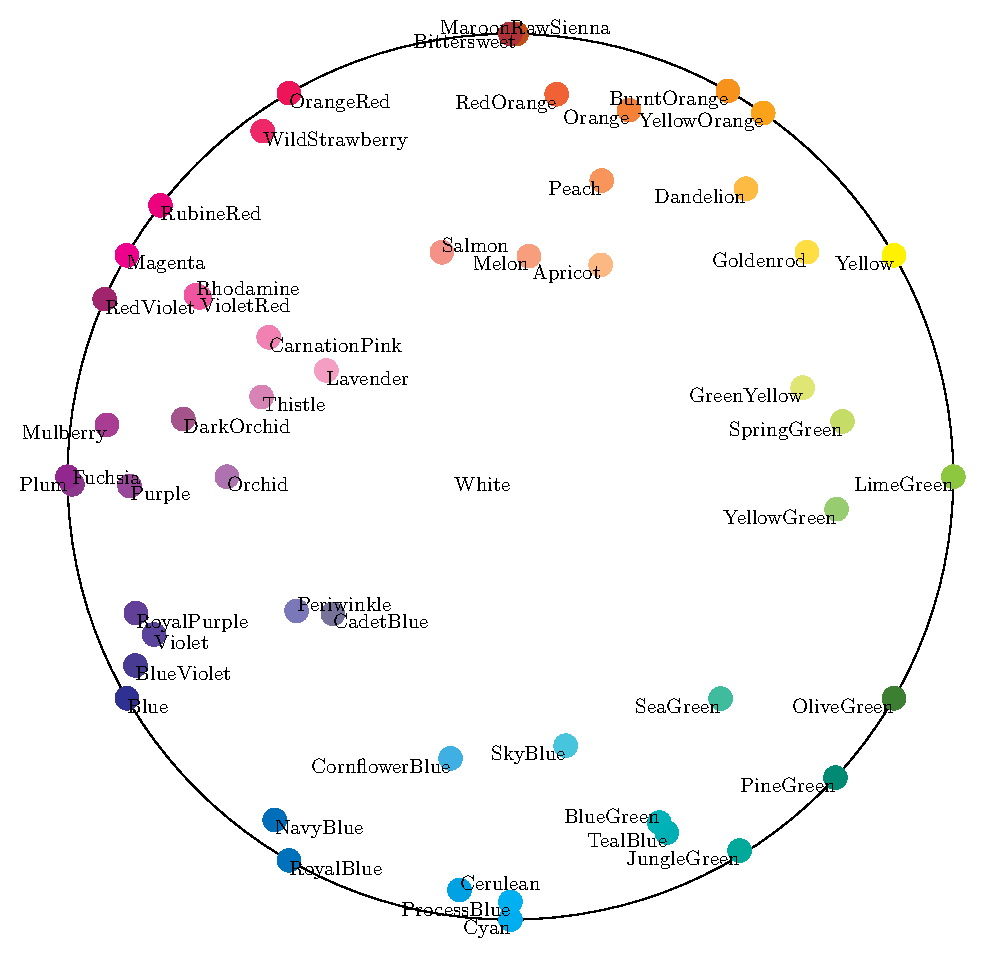
\includegraphics[width=\textwidth]{figures/pyx_colours}
\end{center}
\caption[The named colours which PyXPlot recognises, arranged in HSB colour space]
{The named colours which PyXPlot recognises, arranged in HSB colour space, with the brightness axis orientated into the page. Some colours are not shown as they lie too close to others.}
\label{fig:colour_table3}
\end{figure}


% LINESTYLES.TEX
%
% The documentation in this file is part of PyXPlot
% <http://www.pyxplot.org.uk>
%
% Copyright (C) 2006-2010 Dominic Ford <coders@pyxplot.org.uk>
%               2009-2010 Ross Church
%
% $Id$
%
% PyXPlot is free software; you can redistribute it and/or modify it under the
% terms of the GNU General Public License as published by the Free Software
% Foundation; either version 2 of the License, or (at your option) any later
% version.
%
% You should have received a copy of the GNU General Public License along with
% PyXPlot; if not, write to the Free Software Foundation, Inc., 51 Franklin
% Street, Fifth Floor, Boston, MA  02110-1301, USA

% ----------------------------------------------------------------------------

% LaTeX source for the PyXPlot Users' Guide

\chapter{Line and Point Types}
\label{ch:linetypes_table}

The table below shows the appearance of each numbered line and point type:

\noindent
\includegraphics[width=\textwidth]{examples/eps/ex_linestyles.eps}


% CONFIGURATION.TEX
%
% The documentation in this file is part of PyXPlot
% <http://www.pyxplot.org.uk>
%
% Copyright (C) 2006-8 Dominic Ford <coders@pyxplot.org.uk>
%               2008   Ross Church
%
% $Id$
%
% PyXPlot is free software; you can redistribute it and/or modify it under the
% terms of the GNU General Public License as published by the Free Software
% Foundation; either version 2 of the License, or (at your option) any later
% version.
%
% You should have received a copy of the GNU General Public License along with
% PyXPlot; if not, write to the Free Software Foundation, Inc., 51 Franklin
% Street, Fifth Floor, Boston, MA  02110-1301, USA

% ----------------------------------------------------------------------------

% LaTeX source for the PyXPlot Users' Guide

\chapter{Configuring PyXPlot}

\section{Overview}

\label{configuration}

As is the case in \gnuplot, PyXPlot can be configured using the \indcmdt{set}
-- for example:

\begin{verbatim}set output 'foo.eps'\end{verbatim}

\noindent would cause plotted output to be written the file {\tt foo.eps}.
Typing {\tt set} on its own returns a list of all recognised configuration
parameters of the \indcmdt{set}. The \indcmdt{unset} may be used to return
settings to their default values; it recognises a similar set of parameter
names, and once again, typing {\tt unset} on its own gives a list of them. The
\indcmdt{show} can be used to display the values of settings.

\section{Configuration Files}
\label{config_files}

PyXPlot can also be configured by means of a configuration file, with filename
{\tt .pyxplotrc}, which is scanned once upon startup. This file may be
placed either in the user's current working directory, or in his home
directory. In the event of both files existing, settings in the former override
those in the latter; in the event of neither file existing, PyXPlot uses its
own default settings.

The configuration file should take the form of a series of sections, each
headed by a section heading enclosed in square brackets, and followed by
variables declared using the format:

\begin{verbatim} 
OUTPUT=foo.eps
\end{verbatim}

The following sections are used, although they do not all need to be present in
any given file:

\begin{itemize}
\item {\tt settings} -- contains parameters similar to those which can be set
with the {\tt set} command. A complete list is given in
Section~\ref{configfile_settings} below.
\item {\tt terminal} -- contains parameters for altering the behaviour and
appearance of PyXPlot's interactive terminal. A complete list is given in
Section~\ref{configfile_terminal}.
\item {\tt variables} -- contains variable definitions. Any variables defined
in this section will be predefined in the PyXPlot mathematical environment upon
startup.
\item {\tt functions} -- contains function definitions.
\item {\tt colours} -- contains a variable `{\tt palette}', which should be set
to a comma-separated list of the sequence of colours in the palette used to
plot datasets. The first will be called colour 1 in PyXPlot, the second colour
2, etc. A list of recognised colour names is given in
Section~\ref{colour_names}.
\item {\tt latex} -- contains a variable `{\tt preamble}', which is prefixed to
the beginning of all \LaTeX\ text items, before the {\tt \textbackslash
begin\{document\}} statement. It can be used to define custom \LaTeX\ macros,
or to include packages using the {\tt \textbackslash includepackage\{\}}
command.  The preamble can be changed using the \indcmdt{set preamble}.
\end{itemize}

\section{An Example Configuration File}
\index{configuration files}
\noindent As an example, the following is a configuration file
which would represent PyXPlot's default configuration:

\begin{verbatim}
[settings]
ASPECT=1.0
AUTOASPECT=ON
AXESCOLOUR=Black
BACKUP=OFF
BAR=1.0
BINORIGIN=0
BINWIDTH=1
BOXFROM=0
BOXWIDTH=0
COLOUR=ON
DATASTYLE=points
DISPLAY=ON
DPI=300
ENLARGE=OFF
FONTSIZE=0
FUNCSTYLE=lines
GRID=OFF
GRIDAXISX=1
GRIDAXISY=1
GRIDMAJCOLOUR=Grey60
GRIDMINCOLOUR=Grey90
KEY=ON
KEYCOLUMNS=1
KEYPOS=TOP RIGHT
KEY_XOFF=0.0
KEY_YOFF=0.0
LANDSCAPE=OFF
LINEWIDTH=1.0
MULTIPLOT=OFF
ORIGINX=0.0
ORIGINY=0.0
OUTPUT=
PAPERHEIGHT=297
PAPERWIDTH=210
POINTLINEWIDTH=1.0
POINTSIZE=1.0 
SAMPLES=250
TERMANTIALIAS=ON
TERMENLARGE=OFF
TERMINVERT=OFF
TERMTRANSPARENT=OFF
TERMTYPE=X11_singlewindow
TEXTCOLOUR=Black
TEXTHALIGN=Left
TEXTVALIGN=Bottom
TITLE=
TITLE_XOFF=0.0
TITLE_YOFF=0.0
WIDTH=8.0

[terminal]
COLOUR=OFF
COLOUR_ERR=Red
COLOUR_REP=Green
COLOUR_WRN=Brown
SPLASH=ON

[variables]
pi = 3.14159265358979

[colours]
palette = Black, Red, Blue, Magenta, Cyan, Brown, Salmon, Gray,
Green, NavyBlue, Periwinkle, PineGreen, SeaGreen, GreenYellow,
Orange, CarnationPink, Plum

[latex]
PREAMBLE=
\end{verbatim}

\section{Configuration Options: {\tt settings} section}
\label{configfile_settings}

The following table provides a brief description of the function of each of the
parameters in the {\tt settings} section of the above configuration file,
with a list of possible values for each:

\begin{longtable}{p{3.4cm}p{9cm}}
{\tt ASPECT} & {\bf Possible values:} Any floating-point number.

               {\bf Analogous set command:} \indcmdts{set size ratio}

               Sets the aspect ratio of plots.
               \\
{\tt AUTOASPECT} & {\bf Possible values:} {\tt ON} / {\tt OFF}

               {\bf Analogous set command:} {\tt set size ratio}

               Sets whether plots have the automatic aspect ratio, which is the golden ratio. If {\tt ON}, then the above setting is ignored.
               \\
{\tt AXESCOLOUR} & {\bf Possible values:} Any recognised colour.

               {\bf Analogous set command:} \indcmdts{set axescolour}

               Sets the colour of axis lines and ticks.
               \\
{\tt BACKUP} & {\bf Possible values:} {\tt ON} / {\tt OFF}

               {\bf Analogous set command:} \indcmdts{set backup}

               When this switch is set to `{\tt ON}', and plot output is being directed to file, attempts to write output over existing files cause a copy of the existing file to be preserved, with a tilde after its old filename (see Section~\ref{filebackup}).
               \\
{\tt BAR}     & {\bf Possible values:}  Any floating-point number.

               {\bf Analogous set command:} \indcmdts{set bar}

               Sets the horizontal length of the lines drawn at the end of errorbars, in units of their default length.
               \\
{\tt BINORIGIN} & {\bf Possible values:} Any floating-point number

               {\bf Analogous set command:} \indcmdts{set binorigin}

               Sets the point along the $x$ axis from which the bins used by the \indcmdt{histogram} originate.
               \\
{\tt BINWIDTH} & {\bf Possible values:} Any floating-point number

               {\bf Analogous set command:} \indcmdts{set binwidth}

               Sets the widths of the bins used by the \indcmdt{histogram}.
               \\
{\tt BOXFROM} & {\bf Possible values:} Any floating-point number.

               {\bf Analogous set command:} \indcmdts{set boxfrom}

               Sets the horizontal point from which bars on bar charts appear to emanate.
               \\
{\tt BOXWIDTH} & {\bf Possible values:} Any floating-point number.

               {\bf Analogous set command:} \indcmdts{set boxwidth}

               Sets the default width of boxes on barcharts. If negative, then the boxes have automatically selected widths, so that the interfaces between bars occur at the horizontal midpoints between the specified datapoints.
               \\
{\tt COLOUR} & {\bf Possible values:} {\tt ON} / {\tt OFF}

               {\bf Analogous set command:} \indcmdts{set terminal}

               Sets whether output should be colour ({\tt ON}) or monochrome ({\tt OFF}).
               \\
{\tt DATASTYLE} & {\bf Possible values:} Any plot style. 

               {\bf Analogous set command:} \indcmdts{set data style}
                   
               Sets the plot style used by default when plotting \datafile s.
               \\
{\tt DISPLAY} & {\bf Possible values:} {\tt ON} / {\tt OFF}

               {\bf Analogous set command:} \indcmdts{set display}

               When set to `{\tt ON}', no output is produced until the \indcmdt{set display} is issued. This is useful for speeding up scripts which produce large multiplots; see Section~\ref{set_display} for more details.
               \\
{\tt DPI} & {\bf Possible values:} Any floating-point number.

               {\bf Analogous set command:} \indcmdts{set dpi}

               Sets the sampling quality used, in dots per inch, when output is sent to a bitmapped terminal (the jpeg/gif/png terminals).
               \\
{\tt FONTSIZE} & {\bf Possible values:} Integers in the range $-4 \to 5$.

               {\bf Analogous set command:} \indcmdts{set fontsize}

               Sets the fontsize of text, varying between \LaTeX's {\tt tiny} ($-4$) and {\tt Huge} (5).
               \\
{\tt FUNCSTYLE} & {\bf Possible values:} Any plot style.

               {\bf Analogous set command:} \indcmdts{set function style}

               Sets the plot style used by default when plotting functions.
               \\
{\tt GRID} & {\bf Possible values:} {\tt ON} / {\tt OFF}

               {\bf Analogous set command:} \indcmdts{set grid}

               Sets whether a grid should be displayed on plots.
               \\
{\tt GRIDAXISX} & {\bf Possible values:} Any integer.

               {\bf Analogous set command:} None

               Sets the default $x$-axis to which gridlines should attach, if the {\tt set grid} command is called without specifying which axes to use.
               \\
{\tt GRIDAXISY} & {\bf Possible values:} Any integer.

               {\bf Analogous set command:} None

               Sets the default $y$-axis to which gridlines should attach, if the {\tt set grid} command is called without specifying which axes to use.
               \\
{\tt GRIDMAJCOLOUR} & {\bf Possible values:} Any recognised colour.

               {\bf Analogous set command:} \indcmdts{set gridmajcolour}

               Sets the colour of major grid lines.
               \\
{\tt GRIDMINCOLOUR} & {\bf Possible values:} Any recognised colour.

               {\bf Analogous set command:} \indcmdts{set gridmincolour}

               Sets the colour of minor grid lines.
               \\
{\tt KEY} & {\bf Possible values:} {\tt ON} / {\tt OFF}

               {\bf Analogous set command:} \indcmdts{set key}

               Sets whether a legend is displayed on plots.
               \\
{\tt KEYCOLUMNS} & {\bf Possible values:} Any integer $>0$.

               {\bf Analogous set command:} \indcmdts{set keycolumns}

               Sets the number of columns into which the legends of plots should be divided.
               \\
{\tt KEYPOS} & {\bf Possible values:} `TOP RIGHT', `TOP MIDDLE', `TOP LEFT', `MIDDLE RIGHT', `MIDDLE MIDDLE', `MIDDLE LEFT', `BOTTOM RIGHT', `BOTTOM MIDDLE', `BOTTOM LEFT', `BELOW', `OUTSIDE'.

               {\bf Analogous set command:} \indcmdts{set key}

               Sets where the legend should appear on plots.
               \\
{\tt KEY\_XOFF} & {\bf Possible values:} Any floating-point number.

               {\bf Analogous set command:} \indcmdts{set key}

               Sets the horizontal offset, in approximate graph-widths, that should be applied to the legend, relative to its default position, as set by {\tt KEYPOS}.
               \\
{\tt KEY\_YOFF} & {\bf Possible values:} Any floating-point number.

               {\bf Analogous set command:} \indcmdts{set key}

               Sets the vertical offset, in approximate graph-heights, that should be applied to the legend, relative to its default position, as set by {\tt KEYPOS}.
               \\
{\tt LANDSCAPE} & {\bf Possible values:} {\tt ON} / {\tt OFF}

               {\bf Analogous set command:} \indcmdts{set terminal}

               Sets whether output is in portrait orientation ({\tt OFF}), or landscape orientation ({\tt ON}).
               \\
{\tt LINEWIDTH} & {\bf Possible values:} Any floating-point number.

               {\bf Analogous set command:} \indcmdts{set linewidth}

               Sets the width of lines on plots, as a  multiple of the default.
               \\
{\tt MULTIPLOT} & {\bf Possible values:} {\tt ON} / {\tt OFF}

               {\bf Analogous set command:} \indcmdts{set multiplot}

               Sets whether multiplot mode is on or off.
               \\
{\tt ORIGINX} & {\bf Possible values:} Any floating point number.

               {\bf Analogous set command:} \indcmdts{set origin}

               Sets the horizontal position, in centimetres, of the default origin of plots on the page. Most useful when multiplotting many plots.
               \\
{\tt ORIGINY} & {\bf Possible values:} Any floating point number.

               {\bf Analogous set command:} \indcmdts{set origin}

               Sets the vertical position, in centimetres, of the default origin of plots on the page. Most useful when multiplotting many plots.
               \\
{\tt OUTPUT} & {\bf Possible values:} Any string.

               {\bf Analogous set command:} \indcmdts{set output}

               Sets the output filename for plots. If blank, the default filename of pyxplot.foo is used, where `foo' is an extension appropriate for the file format.
               \\
{\tt PAPER\_HEIGHT} & {\bf Possible values:} Any floating-point number.

               {\bf Analogous set command:} \indcmdts{set papersize}

               Sets the height of the papersize for postscript output in millimetres.
               \\
{\tt PAPER\_NAME} & {\bf Possible values:} A string matching any of the papersizes listed in Table~\ref{paper_sizes}.

               {\bf Analogous set command:} \indcmdts{set papersize}

               Sets the papersize for postscript output to one of the pre-defined papersizes listed in Table~\ref{paper_sizes}.
               \\
{\tt PAPER\_WIDTH} & {\bf Possible values:} Any floating-point number.

               {\bf Analogous set command:} \indcmdts{set papersize}

               Sets the width of the papersize for postscript output in millimetres.
               \\
{\tt POINTLINEWIDTH} & {\bf Possible values:} Any floating-point number.

               {\bf Analogous set command:} \indcmdts{set pointlinewidth}

               Sets the linewidth used to stroke points onto plots, as a multiple of the default.
               \\
{\tt POINTSIZE} & {\bf Possible values:} Any floating-point number.

               {\bf Analogous set command:} \indcmdts{set pointsize}

               Sets the sizes of points on plots, as a multiple of their normal sizes.
               \\
{\tt SAMPLES} & {\bf Possible values:} Any integer.

               {\bf Analogous set command:} \indcmdts{set samples}

               Sets the number of samples (datapoints) to be evaluated along the $x$-axis when plotting a function.
               \\
{\tt TERMANTIALIAS} & {\bf Possible values:} {\tt ON} / {\tt OFF}

               {\bf Analogous set command:} \indcmdts{set terminal}

               Sets whether jpeg/gif/png output is antialiased, i.e.\ whether colour boundaries are smoothed to disguise the effects of pixelisation.
               \\
{\tt TERMENLARGE} & {\bf Possible values:} {\tt ON} / {\tt OFF}

               {\bf Analogous set command:} \indcmdts{set terminal}

               When set to `{\tt ON}' output is enlarged or shrunk to fit the current paper size.
               \\

{\tt TERMINVERT} & {\bf Possible values:} {\tt ON} / {\tt OFF}

               {\bf Analogous set command:} \indcmdts{set terminal}

               Sets whether jpeg/gif/png output has normal colours ({\tt OFF}), or inverted colours ({\tt ON}).
               \\
{\tt TERMTRANSPARENT} & {\bf Possible values:} {\tt ON} / {\tt OFF}

               {\bf Analogous set command:} \indcmdts{set terminal}

               Sets whether jpeg/gif/png output has transparent background ({\tt ON}), or solid background ({\tt OFF}).
               \\
{\tt TERMTYPE} & {\bf Possible values:} {\tt X11\_singlewindow},

               {\tt X11\_multiwindow}, {\tt X11\_persist}, {\tt PS}, {\tt EPS}, {\tt PDF}, {\tt PNG}, {\tt JPG}, {\tt GIF}

               {\bf Analogous set command:} \indcmdts{set terminal}

               Sets whether output is sent to the screen or to disk, and, in the latter case, the format of the output. The {\tt ps} option should be used for both encapsulated and normal postscript output; these are distinguished using the {\tt ENHANCED} option, above.
               \\
{\tt TEXTCOLOUR} & {\bf Possible values:} Any recognised colour.

               {\bf Analogous set command:} \indcmdts{set textcolour}

               Sets the colour of all text output.
               \\
{\tt TEXTHALIGN} & {\bf Possible values:} {\tt Left}, {\tt Centre}, {\tt Right}

               {\bf Analogous set command:} \indcmdts{set texthalign}

               Sets the horizontal alignment of text labels to their given reference positions.
               \\
{\tt TEXTVALIGN} & {\bf Possible values:} {\tt Top}, {\tt Centre}, {\tt Bottom}

               {\bf Analogous set command:} \indcmdts{set textvalign}

               Sets the vertical alignment of text labels to their given reference positions.
               \\
{\tt TITLE} & {\bf Possible values:} Any string.

               {\bf Analogous set command:} \indcmdts{set title}

               Sets the title to appear at the top of the plot.
               \\
{\tt TITLE\_XOFF} & {\bf Possible values:} Any floating point number.

               {\bf Analogous set command:} \indcmdts{set title}

               Sets the horizontal offset of the title of the plot from its default central location.
               \\
{\tt TITLE\_YOFF} & {\bf Possible values:} Any floating point number.

               {\bf Analogous set command:} \indcmdts{set title}

               Sets the vertical offset of the title of the plot from its default location at the top of the plot.
               \\
{\tt WIDTH} & {\bf Possible values:} Any floating-point number.

               {\bf Analogous set command:} \indcmdts{set width} / \indcmdts{set size}

               Sets the width of plots in centimetres.
               \\
\end{longtable}

\section{Configuration Options: {\tt terminal} section}
\label{configfile_terminal}

The following table provides a brief description of the function of each of the
parameters in the {\tt terminal} section of the above configuration file,
with a list of possible values for each:

\begin{longtable}{p{3.4cm}p{9cm}}
{\tt COLOUR} & {\bf Possible values:} {\tt ON} / {\tt OFF}

               {\bf Analogous command-line switches:} {\tt -c}, {\tt --colour}, {\tt -m}, {\tt --monochrome}

               Sets whether colour highlighting should be used in the interactive terminal. If turned on, output is displayed in green, warning messages in amber, and error messages in red; these colours are configurable, as described below. Note that not all UNIX terminals support the use of colour.
               \\
{\tt COLOUR\_ERR} & {\bf Possible values:} Any recognised terminal colour.

               {\bf Analogous command-line switches:} None.

               Sets the colour in which error messages are displayed when colour highlighting is used. Note that the list of recognised colour names differs from that used in PyXPlot; a list is given at the end of this section.
               \\
{\tt COLOUR\_REP} & {\bf Possible values:} Any recognised terminal colour.

               {\bf Analogous command-line switches:} None.

               As above, but sets the colour in which PyXPlot displays its non-error-related output.
               \\
{\tt COLOUR\_WRN} & {\bf Possible values:} Any recognised terminal colour.

               {\bf Analogous command-line switches:} None.

               As above, but sets the colour in which PyXPlot displays its warning messages.
               \\
{\tt SPLASH} & {\bf Possible values:} {\tt ON} / {\tt OFF}

               {\bf Analogous command-line switches:} {\tt -q}, {\tt --quiet}, {\tt -V}, {\tt --verbose}

               Sets whether the standard welcome message is displayed upon startup.
               \\
\end{longtable}

The colours recognised by the {\tt COLOUR\_XXX} configuration options above are: {\tt Red}, {\tt Green}, {\tt Brown}, {\tt Blue}, {\tt Purple}, {\tt Magenta}, {\tt Cyan}, {\tt White}, {\tt Normal}. The final option produces the default foreground colour of your terminal.

\section{Recognised Colour Names}
\label{colour_names}

The following is a complete list of the colour names which PyXPlot recognises in the {\tt set textcolour}, {\tt set axescolour} commands, and in the {\tt colours} section of its configuration file. It should be noted that they are case-insensitive.

\vspace{5mm}\noindent
\index{configuration file!colours}\index{colours!configuration file}
{\tt
GreenYellow, Yellow, Goldenrod, Dandelion, Apricot, Peach, Melon, YellowOrange, Orange, BurntOrange, Bittersweet, RedOrange, Mahogany, Maroon, BrickRed, Red, OrangeRed, RubineRed, WildStrawberry, Salmon, CarnationPink, Magenta, VioletRed, Rhodamine, Mulberry, RedViolet, Fuchsia, Lavender, Thistle, Orchid, DarkOrchid, Purple, Plum, Violet, RoyalPurple, BlueViolet, Periwinkle, CadetBlue, CornflowerBlue, MidnightBlue, NavyBlue, RoyalBlue, Blue, Cerulean, Cyan, ProcessBlue, SkyBlue, Turquoise, TealBlue, Aquamarine, BlueGreen, Emerald, JungleGreen, SeaGreen, Green, ForestGreen, PineGreen, LimeGreen, YellowGreen, SpringGreen, OliveGreen, RawSienna, Sepia, Brown, Tan, Gray, Grey, Black, White, white, black.
}

\vspace{5mm}
The following further colours provide a scale of shades of grey from dark to light, also case-insensitive.

\vspace{5mm}\noindent
\index{colours!shades of grey}
{\tt
grey05, grey10, grey15, grey20, grey25, grey30, grey35, grey40, grey45, grey50, grey55, grey60, grey65, grey70, grey75, grey80, grey85, grey90, grey95.
}

\vspace{5mm}\noindent
The US spelling of grey, ``gray'', is also accepted.

For a colour chart, the reader is referred to Appendix~\ref{colour_charts}, or to Appendix~B of the {\it PyX Reference Manual}.\footnote{\url{http://pyx.sourceforge.net/manual/colorname.html}}

\appendix
% OTHER_APPS.TEX
%
% The documentation in this file is part of PyXPlot
% <http://www.pyxplot.org.uk>
%
% Copyright (C) 2006-2010 Dominic Ford <coders@pyxplot.org.uk>
%               2009-2010 Ross Church
%
% $Id$
%
% PyXPlot is free software; you can redistribute it and/or modify it under the
% terms of the GNU General Public License as published by the Free Software
% Foundation; either version 2 of the License, or (at your option) any later
% version.
%
% You should have received a copy of the GNU General Public License along with
% PyXPlot; if not, write to the Free Software Foundation, Inc., 51 Franklin
% Street, Fifth Floor, Boston, MA  02110-1301, USA

% ----------------------------------------------------------------------------

% LaTeX source for the PyXPlot Users' Guide

\chapter{Other Applications of PyXPlot}

In this chapter we present a short cookbook describing a few common yet
miscellaneous tasks for which PyXPlot may prove useful.

\section{Conversion of JPEG Images to Postscript}
\index{jpeg images}

The need to convert bitmap images -- for example, those in jpeg format -- into
postscript representations is commonly encountered by users of the \LaTeX\
typesetting system, since \LaTeX's {\tt includegraphics} command can only
incorporate encapsulated postscript images into documents.  A small number of
graphics packages provide facilities for making such conversions, including
ImageMagick\index{ImageMagick}'s {\tt convert} command, but these almost
invariable produce excessively large postscript files on account of their
failure to use postscript's native facilities for image compression. PyXPlot's
\indcmdt{image} can in many cases perform much more efficient conversion:

\begin{verbatim}
set output image.eps
image 'image.jpg' width 10
\end{verbatim}

\section{Inserting Equations in Powerpoint Presentations}
\index{Microsoft Powerpoint}\index{presentations}

The two tools most commonly used for presenting talks\index{presentations} --
Microsoft {\it Powerpoint}\index{Microsoft Powerpoint} and
OpenOffice\index{OpenOffice} {\it Impress} -- have limited facilities for importing
text rendered in \LaTeX\ into slides. {\it Powerpoint} does
include its own {\it Equation Editor}, but its output is considerably less
professional than that produced by \LaTeX.  This can prove a frustration for
anyone who works in a field with notation which makes use of non-standard
characters, but especially for those who work in mathematical and
equation-centric disciplines.

It is possible to import graphic images into {\it Powerpoint}, but it cannot
read images in postscript format, the format in which \LaTeX\ usually produces
its output.  PyXPlot's {\tt gif} and {\tt png} terminals provide a fix for this
problem, as the following example demonstrates:

\begin{verbatim}
set term transparent noantialias gif
set term dpi 300
set output 'equation.gif'
set multiplot

# Render the Planck blackbody formula in LaTeX
set textcolour yellow
text '$B_\nu = \frac{8\pi h}{c^3} \
\frac{\nu^3}{\exp \left( h\nu / kT \right) -1 }$' at 0,0
text 'The Planck Blackbody Formula:' at 0 , 0.75
\end{verbatim}

The result is a {\tt gif} image of the desired equation, with yellow text on a
transparent background. This can readily be imported into {\it Powerpoint} and
re-scaled to the desired size.

\section{Delivering Talks in PyXPlot}

Going one step further, PyXPlot can be used as a stand-alone tool for designing
slides for talks; it has several advantages over other presentation tools.  All
of the text which is placed on slides is rendered neatly in \LaTeX.  Images can
be placed on slides using the \indcmdts{jpeg} and \indcmdts{eps} commands, and
placed at any arbitrary coordinate position on the slide.  In comparison with
programs such as Microsoft {\it Powerpoint}\index{Microsoft Powerpoint} and
OpenOffice\index{OpenOffice} {\it Impress}, the text looks much neater,
especially if equations or unusual characters are required. In comparison with
\TeX-based programs such as Foil\TeX, it is much easier to incorporate images
around text to create colourful slides which will keep an audience attentive.

As an additional advantage, graphs can be plotted within the scripts describing
each slide, directly from \datafile s in your local filesystem. If you receive
new data shortly before giving a talk, it is a simple matter to re-run the
PyXPlot scripts and your slides will automatically pick up the new \datafile s.

Below, we outline our recipe for designing slides in PyXPlot. There are many
steps, but they do not take much time; many simply involve pasting text into
various files. Readers of the printed version of the manual may find it easier
to copy these files from the HTML version of this manual on the PyXPlot
website.

\subsection{Setting up Infrastructure}

First, a bit of infrastructure needs to be set up. Note that once this has been
done for one talk, the infrastructure can be copied directly from a previous
talk.

\begin{enumerate}
\item Make a new directory in which to put your talk:
\begin{verbatim}
mkdir my_talk
cd my_talk
\end{verbatim}
\item Make a directory into which you will put the PyXPlot scripts for your
individual slides:
\begin{verbatim}
mkdir scripts
\end{verbatim}
\item Make a directory into which you will put any graphic images which you
want to put into your talk to make it look pretty:
\begin{verbatim}
mkdir images
\end{verbatim}
\item Make a directory into which PyXPlot will put graphic images of your
slides:
\begin{verbatim}
mkdir slides
\end{verbatim}
\item Design a background for your slides. Open a paint program such as the
{\tt gimp}, create a new image which measures $1024\times768$\,pixels, and fill
it with colour. My preference tends to be for a blue colour gradient, running
from bright blue at the top to dark blue at the bottom, but you may be more
inventive than me. You may wish to add institutional and/or project logos in
the corners. Alternatively, you can download a ready-made background image from
the PyXPlot website: \url{http://foo}. You should store this image as {\tt
images/background.jpg}.
\item We need a simple PyXPlot script to set up a slide template. Paste the
following text into the file {\tt scripts/slide\_init}; there's a bit of black
magic in the {\tt arrow} commands in this script which it isn't necessary to
understand at this stage:\label{stp:presentation_magic}
\begin{verbatim}
scale  = 1.25        ; inch = 2.54 # cm
width  = 10.24*scale ; height =  7.68*scale
x = width/100.0      ; y = height/100.0
set term gif ; set dpi (1024.0/width) * inch
set multiplot ; set nodisplay
set texthalign centre ; set textvalign centre
set textcolour yellow
jpeg "images/background.jpg" width width
arrow -x* 25,-y* 25 to -x* 25, y*125 with nohead
arrow -x* 25, y*125 to  x*125, y*125 with nohead
arrow  x*125, y*125 to  x*125,-y* 25 with nohead
arrow  x*125,-y* 25 to -x* 25,-y* 25 with nohead
\end{verbatim}
\item We also need a simple PyXPlot script to round off each slide. Paste the
following text into the file {\tt scripts/slide\_finish}:
\begin{verbatim}
set display ; refresh
\end{verbatim}
\item Paste the following text into the file {\tt compile}. This is a simple
shell script which instructs {\tt pyxplot\_watch} to compile your slides using
PyXPlot every time you edit any of the them:
\begin{verbatim}
#!/bin/bash
pyxplot_watch --verbose scripts/0\*
\end{verbatim}
\item Paste the following text into the file {\tt make\_slides}. This is a
simple shell script which crops your slides to measure exactly
$1024\times768$\,pixels, cropping any text boxes which may go off the side of
them. It links up with the black magic of Step~\ref{stp:presentation_magic}:
\begin{verbatim}
#!/bin/bash
mkdir -p slides_cropped
for all in slides/*.gif ; do
convert $all -crop 1024x768+261+198 `echo $all | \
sed 's@slides@slides_cropped@' | sed 's@gif@jpg@'`
done
\end{verbatim}
\item Make the scripts {\tt compile} and {\tt make\_slides} executable:
\begin{verbatim}
chmod 755 compile make_slides
\end{verbatim}
\end{enumerate}

\subsection{Writing A Short Example Talk}

The infrastructure is now completely set up, and you are ready to start
designing slides. We will now design an example talk with three slides.

\begin{enumerate}
\item Run the script {\tt compile} and leave it running in the background.
PyXPlot will then re-run the scripts describing your slides whenever you edit
them.
\item As an example, we will now make a title slide. Paste the following script
into the file {\tt scripts/0001}:
\begin{verbatim}
set output 'slides/0001.gif'
load 'scripts/slide_init'

text '\parbox[t]{10cm}{\center \LARGE \bf \
  A Tutorial in the use of PyXPlot \\ \
  to present Talks \
} ' at x*50, y*75
text '\Large \bf Prof A.N.\ Other' at x*50, y*45
text '\parbox[t]{9cm}{\center \
  Director, \\ \
  Atlantis Island University \
} ' at x*50, y*38
text 'Annual Lecture, 1st January 2010' at x*50, y*22

load 'scripts/slide_finish'
\end{verbatim}
Note that the variables {\tt x} and {\tt y} are defined to be 1~per cent of the
width and height of your slides respectively, such that the bottom-left of each
slide is at $(0,0)$ and the top-right of each slide is at $({\tt 100*x},{\tt
100*y})$.
\item Next we will make a second slide with a series of bullet points. Paste
the following script into the file {\tt scripts/0002}:
\begin{verbatim}
set output 'slides/0002.gif'
load 'scripts/slide_init'

text '\Large \textbf{Talk Overview}' at x*50, y*92
text "\parbox[t]{9cm}{\begin{itemize} \
 \item Setting up the Infrastructure. \
 \item Writing a Short Example Talk. \
 \item Delivering your Talk. \
 \item Conclusion. \
 \end{itemize} \
} " at x*50 , y*60

set textcol cyan
text '{\bf With thanks to my collaborator, \
           Prof Y.E.\ Tanother.}' at x*50,y*15

load 'scripts/slide_finish'
\end{verbatim}
\item Finally, we will make a third slide with a graph on it. Paste the
following script into the file {\tt scripts/0003}:
\begin{verbatim}
set output 'slides/0003.gif'
load 'scripts/slide_init'

text '\Large \bf The Results of Our Model' at x*50, y*92
set axescolour yellow ; set nogrid
set origin x*17.5, y*20 ; set width x*70
set xrange [0.01:0.7]
set xlabel '$x$'
set yrange [0.01:0.7]
set ylabel '$f(x)$'
set palette Red, Green, Orange, Purple

set key top left
plot x t 'Model 1', exp(x)-1 t 'Model 2', \
     log(x+1) t 'Model 3', sin(x) t 'Model 4'

load 'scripts/slide_finish'
\end{verbatim}
\item To view your slides, run the script {\tt make\_slides}. Afterwards, you
will find your slides as a series of $1024\times768$\,pixel jpeg images in the
directory {\tt slides\_cropped}.  If you have the {\it Quick Image
Viewer}\index{Quick Image Viewer} ({\tt qiv}) installed, then you can view them
as follows:
\begin{verbatim}
qiv slides_cropped/*
\end{verbatim}
If you're in a hurry, you can skip the step of running the script {\tt
make\_slides} and view your slides as images in the {\tt slides} directory, but
note that the slides in here may not be properly cropped. This approach is
generally preferable when viewing your slides in a semi-live fashion as you are
editing them.
\item If you'd like to make the text on your slides larger or smaller, you can
do so by varying the {\tt scale} parameter in the file {\tt
scripts/slide\_init}.
\end{enumerate}

%The three slides which we have designed can been seen in
%Figures~\ref{fig:presentation_slide1}, \ref{fig:presentation_slide2} and
%\ref{fig:presentation_slide3}.

\subsection{Delivering your Talk}

There are two straightforward ways in which you can give your talk. The
quickest way is simply to use the {\it Quick Image Viewer}\index{Quick Image
Viewer} ({\tt qiv}):
\begin{verbatim}
qiv slides_cropped/*
\end{verbatim}
Press the left mouse button to move forward through your talk, and the right
mouse button to go back a slide.

This method does lack some of the niceties of Microsoft {\it Powerpoint} -- for
example, the ability to jump to any arbitrary slide number, compatibility with
wireless remote controls to advance your slides, and the ability to use
animated slide transitions. It may be preferably, therefore, to paste the jpeg
images of your slides into a {\it Powerpoint} or OpenOffice {\it Impress}
presentation before you give your talk.


% GNUPLOT_DIFFS.TEX
%
% The documentation in this file is part of PyXPlot
% <http://www.pyxplot.org.uk>
%
% Copyright (C) 2006-2010 Dominic Ford <coders@pyxplot.org.uk>
%               2008-2010 Ross Church
%
% $Id$
%
% PyXPlot is free software; you can redistribute it and/or modify it under the
% terms of the GNU General Public License as published by the Free Software
% Foundation; either version 2 of the License, or (at your option) any later
% version.
%
% You should have received a copy of the GNU General Public License along with
% PyXPlot; if not, write to the Free Software Foundation, Inc., 51 Franklin
% Street, Fifth Floor, Boston, MA  02110-1301, USA

% ----------------------------------------------------------------------------

% LaTeX source for the PyXPlot Users' Guide

\chapter{Summary of Differences Between PyXPlot and \gnuplot}
\chaptermark{Differences Between PyXPlot \& \gnuplot}
\label{ch:gnuplot_diffs}

PyXPlot's commandline interface is based loosely upon that of \gnuplot, but
does not completely re-implement the entirety of \gnuplot's command language.
Moreover, PyXPlot's command language includes many extensions of \gnuplot's
interface. In this Appendix, we outline some of the most significant areas in
which \gnuplot\ and PyXPlot differ. This is far from an exhaustive list, but
may provide a useful reference for \gnuplot\ users.

\section{The Typesetting of Text}

PyXPlot renders all text labels automatically in the \LaTeX\ typesetting
environment. This brings many advantages: it produces neater labels than the
default typesetting engine used by \gnuplot, makes it straightforward to label
graphs with mathematical expressions, and moreover makes it straightforward
when importing graphs into \LaTeX\ documents to match the fonts used in figures
with those used in the main text of the document.  It does, however, also
necessarily introduce some incompatibility with \gnuplot.  Some strings which
are valid in \gnuplot\ are not valid in PyXPlot (see
Section~\ref{sec:latex_incompatibility} for more details). For
example,\index{latex}

\begin{dontdo}
set xlabel 'x\^{}2'
\end{dontdo}

\noindent is a valid label in \gnuplot, but is not valid input for \LaTeX\ and
therefore fails in PyXPlot.  In PyXPlot, it needs to be written in \LaTeX\
mathmode as:

\begin{dodo}
set xlabel '\$x\^{}2\$'
\end{dodo}

\noindent A useful introduction to \LaTeX's syntax can be found in Tobias
Oetiker's\index{Tobias Oetiker} excellent free tutorial, {\it The Not So Short
Guide to \LaTeX\ $2\epsilon$}\index{Not So Short Guide to \LaTeX\ $2\epsilon$,
The}, which is available for free download from:

\noindent \url{http://www.ctan.org/tex-archive/info/lshort/english/lshort.pdf}

PyXPlot's built-in {\tt texify()} function can also assist by automatically
converting mathematical expressions and  strings of text into \LaTeX, as in the
following examples:

\vspace{3mm}
\noindent{\tt pyxplot> {\bf a=50}}\newline
\noindent{\tt pyxplot> {\bf print texify("A \%d\% increase"\%(a))}}\newline
\noindent{\tt A 50$\backslash$\% increase}\newline
\noindent{\tt pyxplot> {\bf print texify(sqrt(x**2+1))}}\newline
\noindent{\tt \$\\displaystyle $\backslash$sqrt\{x\^{}\{2\}+1\}\$}
\vspace{3mm}

\section{Complex Numbers}

The syntax used for representing complex numbers in PyXPlot differs from that
used in \gnuplot. Whereas \gnuplot\ expects the real and imaginary components
of complex numbers to be represented {\tt \{a,b\}}, PyXPlot uses the syntax
{\tt a+b*i}, assuming that the variable {\tt i} has been defined to equal {\tt
sqrt(-1)}.  In addition, in PyXPlot complex arithmetic must first be enabled
using the {\tt set numerics complex} command before complex numbers may be
entered.  This is illustrated by the following example:

\vspace{3mm}
\noindent{\tt gnuplot> {\bf print \{1,2\} + \{3,4\}}}\newline
\noindent{\tt \{4.0, 6.0\}}
\vspace{3mm}\newline
\noindent{\tt pyxplot> {\bf set numerics complex}}\newline
\noindent{\tt pyxplot> {\bf print (1+2*i) + (3+4*i)}}\newline
\noindent{\tt (4+6i)}
\vspace{3mm}

\section{The Multiplot Environment}

\gnuplot's multiplot environment, used for placing many graphs alongside one
another, is massively extended in PyXPlot.  As well as making it much easier to
produce galleries of plots and inset graphs, a wide range of vector graphs
objects can also be added to the multiplot canvas. This is described in detail
in Chapter~\ref{ch:vector_graphics}.

\section{Plots with Multiple Axes}

In \gnuplot, a maximum of two horizontal and two vertical axes may be
associated with each graph, placed in each case with one on either side of the
plot. These are referred to as the {\tt x} (bottom) and {\tt x2} (top), or {\tt
y} (left) and {\tt y2} (right) axes.  This behaviour is reproduced in PyXPlot,
and so the syntax

\begin{verbatim}
set x2label 'Axis label'
\end{verbatim}

\noindent works similarly in both programs. However, in PyXPlot the position of
each axis may be set individually using syntax such as

\begin{verbatim}
set axis x2 top
\end{verbatim}

\noindent and furthermore up to~128 axes may be placed parallel to one another:

\begin{verbatim}
set axis x127 top
set x127label "This is axis number 127"
\end{verbatim}

\noindent More details of how to configure axes can be found in
Section~\ref{sec:multiple_axes}.

\section{Plotting Parametric Functions}

The syntax used for plotting parametric functions differs between \gnuplot\ and
PyXPlot. Whereas parametric plotting is enabled in \gnuplot\ using the {\tt set
parametric} command, in PyXPlot it is enabled on a per-dataset basis by placing
the keyword {\tt parametric} before the algebraic expression to be plotted:

\vspace{3mm}
\noindent{\tt gnuplot> {\bf set parametric}}\newline
\noindent{\tt gnuplot> {\bf set trange [0:2*pi]}}\newline
\noindent{\tt gnuplot> {\bf plot sin(t),cos(t)}}
\vspace{3mm}\newline
\noindent{\tt pyxplot> {\bf set trange [0:2*pi]}}\newline
\noindent{\tt pyxplot> {\bf plot parametric sin(t):cos(t)}}
\vspace{3mm}

\noindent This makes it straightforward to plot parametric functions alongside
non-parametric functions. For more information, see
Section~\ref{sec:parametric_plotting}.

%\section{Displaying Times and Dates on Axes}


% FIT_MATHS.TEX
%
% The documentation in this file is part of PyXPlot
% <http://www.pyxplot.org.uk>
%
% Copyright (C) 2006-8 Dominic Ford <coders@pyxplot.org.uk>
%               2008   Ross Church
%
% $Id$
%
% PyXPlot is free software; you can redistribute it and/or modify it under the
% terms of the GNU General Public License as published by the Free Software
% Foundation; either version 2 of the License, or (at your option) any later
% version.
%
% You should have received a copy of the GNU General Public License along with
% PyXPlot; if not, write to the Free Software Foundation, Inc., 51 Franklin
% Street, Fifth Floor, Boston, MA  02110-1301, USA

% ----------------------------------------------------------------------------

% LaTeX source for the PyXPlot Users' Guide

\chapter{The {\tt fit} Command: Mathematical Details}
\chaptermark{Details of the {\tt fit} command}
\label{fit_math}

In this section, the mathematical details of the workings of the \indcmdt{fit}
are described. This may be of interest in diagnosing its limitations, and also
in understanding the various quantities that it outputs after a fit is found.
This discussion must necessarily be a rather brief treatment of a large
subject; for a fuller account, the reader is referred to D.S.\ Sivia's {\it
Data Analysis: A Bayesian Tutorial}.

\section{Notation}
\label{bayes_notation}

I shall assume that we have some function $f()$, which takes $n_\mathrm{x}$
parameters, $x_0$...$x_{n_\mathrm{x}-1}$, the set of which may collectively be
written as the vector $\mathbf{x}$. We are supplied a datafile, containing a
number $n_\mathrm{d}$ of datapoints, each consisting of a set of values for
each of the $n_\mathrm{x}$ parameters, and one for the value which we are
seeking to make $f(\mathbf{x})$ match. I shall call of parameter values for the
$i$th datapoint $\mathbf{x}_i$, and the corresponding value which we are trying
to match $f_i$. The datafile may contain error estimates for the values $f_i$,
which I shall denote $\sigma_i$. If these are not supplied, then I shall
consider these quantities to be unknown, and equal to some constant
$\sigma_\mathrm{data}$.

Finally, I assume that there are $n_\mathrm{u}$ coefficients within the
function $f()$ that we are able to vary, corresponding to those variable names
listed after the {\tt via} statement in the {\tt fit} command. I shall
call these coefficients $u_0$...$u_{n_\mathrm{u}-1}$, and refer to them
collectively as $\mathbf{u}$.

I model the values $f_i$ in the supplied datafile as being noisy
Gaussian-distributed observations of the true function $f()$, and within this
framework, seek to find that vector of values $\mathbf{u}$ which is most
probable, given these observations. The probability of any given $\mathbf{u}$
is written
$\mathrm{P}\left( \mathbf{u} | \left\{ \mathbf{x}_i, f_i, \sigma_i \right\} \right)$.

\section{The Probability Density Function}
\label{bayes_pdf}

Bayes' Theorem states that:

\begin{equation}
\mathrm{P}\left( \mathbf{u} | \left\{ \mathbf{x}_i, f_i, \sigma_i \right\} \right) =
\frac{
\mathrm{P}\left( \left\{f_i \right\} | \mathbf{u}, \left\{ \mathbf{x}_i, \sigma_i \right\} \right)
\mathrm{P}\left( \mathbf{u} | \left\{ \mathbf{x}_i, \sigma_i \right\} \right)
}{
\mathrm{P}\left( \left\{f_i \right\} | \left\{ \mathbf{x}_i, \sigma_i \right\} \right)
}
\end{equation}

Since we are only seeking to maximise the quantity on the left, and the
denominator, termed the Bayesian \textit{evidence}, is independent of
$\mathbf{u}$, we can neglect it and replace the equality sign with a
proportionality sign.  Furthermore, if we assume a uniform prior, that is, we
assume that we have no prior knowledge to bias us towards certain more favoured
values of $\mathbf{u}$, then $\mathrm{P}\left( \mathbf{u} \right)$ is also a
constant which can be neglected. We conclude that maximising $\mathrm{P}\left(
\mathbf{u} | \left\{ \mathbf{x}_i, f_i, \sigma_i \right\} \right)$ is
equivalent to maximising $\mathrm{P}\left( \left\{f_i \right\} | \mathbf{u},
\left\{ \mathbf{x}_i, \sigma_i \right\} \right)$.

Since we are assuming $f_i$ to be Gaussian-distributed observations of the true
function $f()$, this latter probability can be written as a product of
$n_\mathrm{d}$ Gaussian distributions:

\begin{equation}
\mathrm{P}\left( \left\{f_i \right\} | \mathbf{u}, \left\{ \mathbf{x}_i, \sigma_i \right\} \right)
=
\prod_{i=0}^{n_\mathrm{d}-1} \frac{1}{\sigma_i\sqrt{2\pi}} \exp \left(
\frac{
-\left[f_i - f_\mathbf{u}(\mathbf{x}_i)\right]^2
}{
2 \sigma_i^2
} \right)
\end{equation}

The product in this equation can be converted into a more computationally
workable sum by taking the logarithm of both sides. Since logarithms are
monotonically increasing functions, maximising a probability is equivalent to
maximising its logarithm. We may write the logarithm $L$ of $\mathrm{P}\left(
\mathbf{u} | \left\{ \mathbf{x}_i, f_i, \sigma_i \right\} \right)$ as:

\begin{equation}
L = \sum_{i=0}^{n_\mathrm{d}-1}
\left( \frac{
-\left[f_i - f_\mathbf{u}(\mathbf{x}_i)\right]^2
}{
2 \sigma_i^2
} \right) + k
\end{equation}

\noindent where $k$ is some constant which does not affect the maximisation
process. It is this quantity, the familiar sum-of-square-residuals, that we
numerically maximise to find our best-fitting set of parameters, which I shall
refer to from here on as $\mathbf{u}^0$.

\section{Estimating the Error in $\mathbf{u}^0$}

To estimate the error in the best-fitting parameter values that we find, we
assume $\mathrm{P}\left( \mathbf{u} | \left\{ \mathbf{x}_i, f_i, \sigma_i
\right\} \right)$ to be approximated by an $n_\mathrm{u}$-dimensional Gaussian
distribution around $\mathbf{u}^0$. Taking a Taylor expansion of
$L(\mathbf{u})$ about $\mathbf{u}^0$, we can write:

\begin{eqnarray}
L(\mathbf{u}) & = & L(\mathbf{u}^0) +
    \underbrace{
      \sum_{i=0}^{n_\mathrm{u}-1} \left( u_i - u^0_i \right)
      \left.\frac{\partial L}{\partial u_i}\right|_{\mathbf{u}^0}
    }_{\textrm{Zero at $\mathbf{u}^0$ by definition}} + \label{L_taylor_expand}\\
& & \sum_{i=0}^{n_\mathrm{u}-1} \sum_{j=0}^{n_\mathrm{u}-1} \frac{\left( u_i - u^0_i \right) \left( u_j - u^0_j \right)}{2}
    \left.\frac{\partial^2 L}{\partial u_i \partial u_j}\right|_{\mathbf{u}^0} +
    \mathcal{O}\left( \mathbf{u} - \mathbf{u}^0\right)^3 \nonumber
\end{eqnarray}

Since the logarithm of a Gaussian distribution is a parabola, the quadratic
terms in the above expansion encode the Gaussian component of the probability
distribution $\mathrm{P}\left( \mathbf{u} | \left\{ \mathbf{x}_i, f_i, \sigma_i
\right\} \right)$ about $\mathbf{u}^0$.\footnote{The use of this is called
\textit{Gauss' Method}. Higher order terms in the expansion represent any
non-Gaussianity in the probability distribution, which we neglect. See MacKay,
D.J.C., \textit{Information Theory, Inference and Learning Algorithms}, CUP
(2003).} We may write the sum of these terms, which we denote $Q$, in matrix
form:

\begin{equation}
Q = \frac{1}{2} \left(\mathbf{u} - \mathbf{u}^0\right)^\mathbf{T} \mathbf{A} \left(\mathbf{u} - \mathbf{u}^0\right)
\label{Q_vector}
\end{equation}

\noindent where the superscript $^\mathbf{T}$ represents the transpose of the
vector displacement from $\mathbf{u}^0$, and $\mathbf{A}$ is the Hessian matrix
of $L$, given by:

\begin{equation}
A_{ij} = \nabla\nabla L = \left.\frac{\partial^2 L}{\partial u_i \partial u_j}\right|_{\mathbf{u}^0}
\end{equation}
\index{Hessian matrix}

This is the Hessian matrix which is output by the {\tt fit} command. In
general, an $n_\mathrm{u}$-dimensional Gaussian distribution such as that given
by equation~(\ref{L_taylor_expand}) yields elliptical contours of
equiprobability in parameter space, whose principal axes need not be aligned
with our chosen co-ordinate axes -- the variables $u_0 ... u_{n_u-1}$. The
eigenvectors $\mathbf{e}_i$ of $\mathbf{A}$ are the principal axes of these
ellipses, and the corresponding eigenvalues $\lambda_i$ equal $1/\sigma_i^2$,
where $\sigma_i$ is the standard deviation of the probability density function
along the direction of these axes.

This can be visualised by imagining that we diagonalise $\mathbf{A}$, and
expand equation~(\ref{Q_vector}) in our diagonal basis. The resulting
expression for $L$ is a sum of square terms; the cross terms vanish in this
basis by definition. The equations of the equiprobability contours become the
equations of ellipses:

\begin{equation}
Q = \frac{1}{2} \sum_{i=0}^{n_\mathrm{u}-1} A_{ii} \left(u_i - u^0_i\right)^2 = k
\end{equation}

\noindent where $k$ is some constant. By comparison with the equation for the
logarithm of a Gaussian distribution, we can associate $A_{ii}$ with
$-1/\sigma_i^2$ in our eigenvector basis.

The problem of evaluating the standard deviations of our variables $u_i$ is
more complicated, however, as we are attempting to evaluate the width of these
elliptical equiprobability contours in directions which are, in general, not
aligned with their principal axes. To achieve this, we first convert our
Hessian matrix into a covariance matrix.

\section{The Covariance Matrix}
\index{covariance matrix}

The terms of the covariance matrix $V_{ij}$ are defined by:

\begin{equation}
\label{def_covar}
V_{ij} = \left< \left(u_i - u^0_i\right) \left(u_j - u^0_j\right) \right>
\end{equation}

\noindent Its leading diagonal terms may be recognised as equalling the
variances of each of our $n_\mathrm{u}$ variables; its cross terms measure the
correlation between the variables. If a component $V_{ij} > 0$, it implies that
higher estimates of the coefficient $u_i$ make higher estimates of $u_j$ more
favourable also; if $V_{ij} < 0$, the converse is true.

It is a standard statistical result that $\mathbf{V} = (-\mathbf{A})^{-1}$. In
the remainder of this section we prove this; readers who are willing to accept
this may skip onto Section~\ref{correlation_matrix}.

Using $\Delta u_i$ to denote $\left(u_i - u^0_i\right)$, we may proceed by
rewriting equation~(\ref{def_covar}) as:

\begin{eqnarray}
V_{ij} & = & \idotsint_{u_i=-\infty}^{\infty}
\Delta u_i \Delta u_j
\mathrm{P}\left(
\mathbf{u} | \left\{ \mathbf{x}_i, f_i, \sigma_i \right\} \right)
\,\mathrm{d}^{n_\mathrm{u}}\mathbf{u} \\
 & = & \frac{
\idotsint_{u_i=-\infty}^{\infty} \Delta u_i \Delta u_j \exp(-Q) \,\mathrm{d}^{n_\mathrm{u}}\mathbf{u}
}{
\idotsint_{u_i=-\infty}^{\infty} \exp(-Q) \,\mathrm{d}^{n_\mathrm{u}}\mathbf{u}
}
\nonumber
\end{eqnarray}

The normalisation factor in the denominator of this expression, which we denote
as $Z$, the \textit{partition function}, may be evaluated by
$n_\mathrm{u}$-dimensional Gaussian integration, and is a standard result:

\begin{eqnarray}
Z & = & \idotsint_{u_i=-\infty}^{\infty} \exp\left(\frac{1}{2} \Delta \mathbf{u}^\mathbf{T} \mathbf{A} \Delta \mathbf{u} \right) \,\mathrm{d}^{n_\mathrm{u}}\mathbf{u} \\
& = & \frac{(2\pi)^{n_\mathrm{u}/2}}{\mathrm{Det}(\mathbf{-A})} \nonumber
\end{eqnarray}

Differentiating $\log_e(Z)$ with respect of any given component of the Hessian
matrix $A_{ij}$ yields:

\begin{equation}
-2 \frac{\partial}{\partial A_{ij}} \left[ \log_e(Z) \right] = \frac{1}{Z}
\idotsint_{u_i=-\infty}^{\infty} \Delta u_i \Delta u_j \exp(-Q) \,\mathrm{d}^{n_\mathrm{u}}\mathbf{u}
\end{equation}

\noindent which we may identify as equalling $V_{ij}$:

\begin{eqnarray}
\label{v_zrelate}
V_{ij} & = & -2 \frac{\partial}{\partial A_{ij}} \left[ \log_e(Z) \right] \\
& = & -2 \frac{\partial}{\partial A_{ij}} \left[ \log_e((2\pi)^{n_\mathrm{u}/2}) - \log_e(\mathrm{Det}(\mathbf{-A})) \right] \nonumber \\
& = & 2 \frac{\partial}{\partial A_{ij}} \left[ \log_e(\mathrm{Det}(\mathbf{-A})) \right] \nonumber
\end{eqnarray}

\noindent This expression may be simplified by recalling that the determinant
of a matrix is equal to the scalar product of any of its rows with its
cofactors, yielding the result:

\begin{equation}
\frac{\partial}{\partial A_{ij}} \left[\mathrm{Det}(\mathbf{-A})\right] = -a_{ij}
\end{equation}

\noindent where $a_{ij}$ is the cofactor of $A_{ij}$. Substituting this into
equation~(\ref{v_zrelate}) yields:

\begin{equation}
V_{ij} = \frac{-a_{ij}}{\mathrm{Det}(\mathbf{-A})}
\end{equation}

Recalling that the adjoint $\mathbf{A}^\dagger$ of the Hessian matrix is the
matrix of cofactors of its transpose, and that $\mathbf{A}$ is symmetric, we
may write:

\begin{equation}
V_{ij} = \frac{-\mathbf{A}^\dagger}{\mathrm{Det}(\mathbf{-A})} \equiv (-\mathbf{A})^{-1}
\end{equation}

\noindent which proves the result stated earlier.

\section{The Correlation Matrix}
\label{correlation_matrix}
\index{correlation matrix}

Having evaluated the covariance matrix, we may straightforwardly find the
standard deviations in each of our variables, by taking the square roots of the
terms along its leading diagonal. For datafiles where the user does not specify
the standard deviations $\sigma_i$ in each value $f_i$, the task is not quite
complete, as the Hessian matrix depends critically upon these uncertainties,
even if they are assumed the same for all of our $f_i$. This point is returned
to in Section~\ref{finding_sigmai}.

The correlation matrix $\mathbf{C}$, whose terms are given by:

\begin{equation}
C_{ij} = \frac{V_{ij}}{\sigma_i\sigma_j}
\end{equation}

\noindent may be considered a more user-friendly version of the covariance
matrix for inspecting the correlation between parameters. The leading diagonal
terms are all clearly equal unity by construction. The cross terms lie in the
range $-1 \leq C_{ij} \leq 1$, the upper limit of this range representing
perfect correlation between parameters, and the lower limit perfect
anti-correlation.

\section{Finding $\sigma_i$}
\label{finding_sigmai}

Throughout the preceding sections, the uncertainties in the supplied target
values $f_i$ have been denoted $\sigma_i$ (see Section~\ref{bayes_notation}).
The user has the option of supplying these in the source datafile, in which
case the provisions of the previous sections are now complete; both
best-estimate parameter values and their uncertainties can be calculated. The
user may also, however, leave the uncertainties in $f_i$ unstated, in which
case, as described in Section~\ref{bayes_notation}, we assume all of the data
values to have a common uncertainty $\sigma_\mathrm{data}$, which is an
unknown.

In this case, where $\sigma_i = \sigma_\mathrm{data} \,\forall\, i$, the best
fitting parameter values are independent of $\sigma_\mathrm{data}$, but the
same is not true of the uncertainties in these values, as the terms of the
Hessian matrix do depend upon $\sigma_\mathrm{data}$. We must therefore
undertake a further calculation to find the most probable value of
$\sigma_\mathrm{data}$, given the data. This is achieved by maximising
$\mathrm{P}\left( \sigma_\mathrm{data} | \left\{ \mathbf{x}_i, f_i \right\}
\right)$. Returning once again to Bayes' Theorem, we can write:

\begin{equation}
\mathrm{P}\left( \sigma_\mathrm{data} | \left\{ \mathbf{x}_i, f_i \right\} \right)
= \frac{
\mathrm{P}\left( \left\{ f_i \right\} | \sigma_\mathrm{data}, \left\{ \mathbf{x}_i \right\} \right)
\mathrm{P}\left( \sigma_\mathrm{data} | \left\{ \mathbf{x}_i \right\} \right)
}{
\mathrm{P}\left( \left\{ f_i \right\} | \left\{ \mathbf{x}_i \right\} \right)
}
\end{equation}

As before, we neglect the denominator, which has no effect upon the
maximisation problem, and assume a uniform prior $\mathrm{P}\left(
\sigma_\mathrm{data} | \left\{ \mathbf{x}_i \right\} \right)$. This reduces the
problem to the maximisation of $\mathrm{P}\left( \left\{ f_i \right\} |
\sigma_\mathrm{data}, \left\{ \mathbf{x}_i \right\} \right)$, which we may
write as a marginalised probability distribution over $\mathbf{u}$:

\begin{eqnarray}
\label{p_f_given_sigma}
\mathrm{P}\left( \left\{ f_i \right\} | \sigma_\mathrm{data}, \left\{ \mathbf{x}_i \right\} \right) =
\idotsint_{-\infty}^{\infty}
&
\mathrm{P}\left( \left\{ f_i \right\} | \sigma_\mathrm{data}, \left\{ \mathbf{x}_i \right\}, \mathbf{u} \right)
\times & \\ &
\mathrm{P}\left( \mathbf{u} | \sigma_\mathrm{data}, \left\{ \mathbf{x}_i \right\} \right)
\,\mathrm{d}^{n_\mathrm{u}}\mathbf{u}
& \nonumber
\end{eqnarray}

Assuming a uniform prior for $\mathbf{u}$, we may neglect the latter term in
the integral, but even with this assumption, the integral is not generally
tractable, as $\mathrm{P}\left( \left\{ f_i \right\} | \sigma_\mathrm{data},
\left\{ \mathbf{x}_i \right\}, \left\{ \mathbf{u}_i \right\} \right)$ may well
be multimodal in form. However, if we neglect such possibilities, and assume
this probability distribution to be approximate a Gaussian \textit{globally},
we can make use of the standard result for an $n_\mathrm{u}$-dimensional Gaussian integral:

\begin{equation}
\idotsint_{-\infty}^{\infty}
\exp \left(
\frac{1}{2}\mathbf{u}^\mathbf{T} \mathbf{A} \mathbf{u}
\right) \,\mathrm{d}^{n_\mathrm{u}}\mathbf{u}
=
\frac{
(2\pi)^{n_\mathrm{u}/2}
}{
\sqrt{\mathrm{Det}\left(-\mathbf{A}\right)}
}
\end{equation}

\noindent We may thus approximate equation~(\ref{p_f_given_sigma}) as:

\begin{eqnarray}
\mathrm{P}\left( \left\{ f_i \right\} | \sigma_\mathrm{data}, \left\{ \mathbf{x}_i \right\} \right)
& \approx &
\mathrm{P}\left( \left\{ f_i \right\} | \sigma_\mathrm{data}, \left\{ \mathbf{x}_i \right\}, \mathbf{u}^0 \right)
\times \\
& &
\mathrm{P}\left( \mathbf{u}^0 | \sigma_\mathrm{data}, \left\{ \mathbf{x}_i, f_i \right\} \right)
\frac{
(2\pi)^{n_\mathrm{u}/2}
}{
\sqrt{\mathrm{Det}\left(-\mathbf{A}\right)}
}
\nonumber
\end{eqnarray}

As in Section~\ref{bayes_pdf}, it is numerically easier to maximise this
quantity via its logarithm, which we denote $L_2$, and can write as:

\begin{eqnarray}
L_2 & = &
\sum_{i=0}^{n_\mathrm{d}-1}
\left(
\frac{
-\left[f_i - f_{\mathbf{u}^0}(\mathbf{x}_i)\right]^2
}{
2\sigma_\mathrm{data}^2
}
- \log_e \left(2\pi\sqrt{\sigma_\mathrm{data}} \right)
\right) +
\\ & & \nonumber
\log_e \left(
\frac{
(2\pi)^{n_\mathrm{u}/2}
}{
\sqrt{\mathrm{Det}\left(-\mathbf{A}\right)}
}
\right)
\end{eqnarray}

This quantity is maximised numerically, a process simplified by the fact that
$\mathbf{u}^0$ is independent of $\sigma_\mathrm{data}$.

% CHANGELOG.TEX
%
% The documentation in this file is part of PyXPlot
% <http://www.pyxplot.org.uk>
%
% Copyright (C) 2006-2010 Dominic Ford <coders@pyxplot.org.uk>
%               2009-2010 Ross Church
%
% $Id$
%
% PyXPlot is free software; you can redistribute it and/or modify it under the
% terms of the GNU General Public License as published by the Free Software
% Foundation; either version 2 of the License, or (at your option) any later
% version.
%
% You should have received a copy of the GNU General Public License along with
% PyXPlot; if not, write to the Free Software Foundation, Inc., 51 Franklin
% Street, Fifth Floor, Boston, MA  02110-1301, USA

% ----------------------------------------------------------------------------

% LaTeX source for the PyXPlot Users' Guide

\chapter{ChangeLog}
\index{ChangeLog}

\subsection*{2010 ??? ??: PyXPlot 0.8.0}

\subsubsection*{Summary:}

This release is a major update, for which PyXPlot's original python code has
been completely rewritten in C with the addition of many new features. Because
of the scale of this update, there is some minor syntax incompatibility with
previous versions where features have undergone particularly heavy change. The
most apparent change is the increase in speed and efficiency resultant from the
use of a compiled language: especially when handling large \datafile s, PyXPlot
0.8.0 can run more than an order-of-magnitude faster than previous versions.

\subsubsection*{Details:}

\begin{itemize}
\item The handling of large \datafile s has been streamlined to require around an order-of-magnitude less time and memory.
\item PyXPlot's mathematical environment has been extended to handle complex numbers and quantities with physical units.
\item The range of mathematical functions built into PyXPlot has been massively extended.
\item The {\tt solve} command has been added to allow the solution of systems of equations.
\item The {\tt maximise} and {\tt minimise} commands have been added to allow searches for local extrema of functions.
\item An {\tt fft} command has been added for performing Fourier transforms on data.
\item New plot styles -- {\tt filledregion} and {\tt yerrorshaded} -- have been added for plotting filled error regions.
\item The configuration of linked axes has been entirely redesigned.
\item Parametric function plotting has been implemented.
\item Colours can now be specified by RGB, HSB or CMYK components, as well as by name.
\item Several commands, e.g. {\tt box}, {\tt circle}, {\tt ellipse}, etc., have been added to allow vector graphics to be produced in PyXPlot's multiplot environment.
\item The {\tt jpeg} command has been generalised to allow the incorporation of not only {\tt jpeg} images, but also {\tt bmp}, {\tt gif} and {\tt png} images, onto multiplot canvases. The command has been renamed {\tt image} in recognition of its wider applicability. Image transparency is now supported in {\tt gif} and {\tt png} images.
\item The {\tt spline} command, now renamed the {\tt interpolate} command, has been extended up provide many types of interpolation between datapoints.
\item A wide range of conditional and flow control structures have been added to PyXPlot's command language -- these are the {\tt do}, {\tt for}, {\tt foreach}, {\tt if} and {\tt while} commands and the {\tt cond\-ition\-alS} and {\tt con\-dition\-alN} mathematical functions.
\item Input filters have been introduced as a mechanism by which datafiles in arbitrary formats can be read.
\item PyXPlot's commandline interface now supports tab completion.
\item The {\tt show} command has been reworked to produce pastable output.
\item Many minor bugs have been fixed.
\end{itemize}

\subsection*{2009 May 24: PyXPlot 0.7.1}

\subsubsection*{Summary:}

This release has no major new features, but fixes several serious bugs in version 0.7.0.

\subsubsection*{Details:}

\begin{itemize}
\item The {\tt exec} command did not work in PyXPlot 0.7.0; this issue has been resolved.
\item The {\tt xyerrorrange} plot style did not work in PyXPlot 0.7.0; this issue has been resolved.
\item PyXPlot 0.7.0 produces large numbers of python deprecation error messages when run under python 2.6; the code has been updated to remove references to deprecated python functions.
\end{itemize}

\subsubsection*{Details -- Change of System Requirements:}

\begin{itemize}
\item In order to fix some of the bugs listed above, it has been necessary to
fix bugs in the PyX graphics library as well as those in PyXPlot. As a result,
and to ensure that these bugfixes reach users as quickly as possible, we have
opted to ship our own modified version of PyX 0.10, called dcfPyX with PyXPlot.
\end{itemize}

\subsection*{2008 Oct 14: PyXPlot 0.7.0}

\subsubsection*{Summary:}

Third PyXPlot beta-release. The code has undergone significant streamlining,
and now runs approximately twice as fast as version 0.6.3 when handling large
datafiles. Memory usage has also been radically reduced. Two new data
processing commands have been introduced. The {\tt tabulate} command can be
used to produce textual datafiles, allowing the user to read data in from
files, apply some analysis, and then write the processed data back to file. The
{\tt histogram} command can be used to estimate the frequency densities of sets
of data points, either by binning them into a bar chart, or by fitting a
functional form to their frequency density.

\subsubsection*{Details -- New and Extended Commands:}

\begin{itemize}
\item {\tt tabulate}
\item {\tt histogram}
\item {\tt set label} and {\tt text} commands extended to allow a colour to be
specified.
\end{itemize}

\subsubsection*{Details -- API changes}

\begin{itemize}
\item {\tt diff\_dx()} and {\tt int\_dx()} functions -- the function to be
differentiated or integrated must now be placed in quotation marks.
\end{itemize}

\subsubsection*{Details -- Change of System Requirements:}

\begin{itemize}
\item Requirement of PyX version 0.9 has been updated to PyX version 0.10. Note that new versions of the PyX graphics library are not generally backwardly compatible.
\end{itemize}

\subsection*{2007 Feb 26: PyXPlot 0.6.3}

\subsubsection*{Summary:}

Second PyXPlot beta-release. The most significant change is the introduction of
a new command-line parser, with greatly improved handling of complex
expressions and much more meaningful syntax error messages. Multi-platform
compatibility has also been massively improved, and dependencies loosened.  A
small number of new commands have been added; most notable among them are the
{\tt jpeg} and {\tt eps} commands, which embed images in multiplots.

\subsubsection*{Details -- New and Extended Commands:}

\begin{itemize}
\item {\tt jpeg}
\item {\tt eps}
\item {\tt set xtics} and {\tt set mxtics}
\item {\tt text} and {\tt set label} commands extended to allow text rotation.
\item {\tt set log} command extended to allow the use of logarithms with bases other than 10.
\item {\tt set preamble}
\item {\tt set term enlarge | noenlarge}
\item {\tt set term pdf}
\item {\tt set term x11\_persist}
\end{itemize}

\subsubsection*{Details -- Eased System Requirements:}

\begin{itemize}
\item Requirement on Python 2.4 minimum eased to version 2.3 minimum.
\item Requirements on scipy and readline eased; PyXPlot will now work in reduced form when they are absent, though they are still strongly recommended.
\item dvips and ghostscript are no longer required.
\end{itemize}

\subsubsection*{Details -- Removed Commands:}

Due to a general refinement of PyXPlot's API, some of the less sensible pieces
of syntax from Version~0.5 are no longer supported. The author apologises for
any inconvenience caused.

\begin{itemize}
\item The {\tt delete\_arrow}, {\tt delete\_text}, {\tt move\_text}, {\tt undelete\_arrow} and {\tt undelete\_text} commands have been removed from the PyXPlot API. The {\tt move}, {\tt delete} and {\tt undelete} commands should now be used to act upon all types of multiplot objects.
\item The {\tt set terminal} command no longer accepts the {\tt enhanced} and {\tt noenhanced} modifiers. The {\tt postscript} and {\tt eps} terminals should be used instead.
\item The {\tt select} modifier, used after the {\tt plot}, {\tt replot}, {\tt fit} and {\tt spline} command can now only be used once; to specify multiple {\tt select} criteria, use the {\tt and} logical operator.
\end{itemize}

\subsection*{2006 Sep 09: PyXPlot 0.5.8}

First beta-release.


\printindex
\end{document}
